\documentclass[a4paper,12pt,twoside]{scrreprt}
% Autor der Vorlage: Klaus Rheinberger, FH Vorarlberg, 2017-02-20

%% Pakete
% Dokumenteneigenschaften
\usepackage[ngerman]{babel}                 % Deutsche Sprachanpassungen
\usepackage[T1]{fontenc}                    % Silbentrennung bei Sonderzeichen
\usepackage[bindingoffset=8mm]{geometry}    % Bindeverlust von 8mm einbeziehen
\usepackage{minted}                         % Code Highlighting/Import
\usepackage{setspace}                       % Zeilenabstand

% Bilder & PDFs
\usepackage{graphicx} % Bilder einbinden
\usepackage{wrapfig}  % Bilder positionieren
\usepackage{pdfpages} % PDFs einbetten

% Zitate & Verweise, Sonstiges
\usepackage[nohyperlinks]{acronym}  % Abkürzungsverzeichnis
\usepackage{caption}                % Abbildungslegenden
\usepackage{csquotes}               % Anführungszeichen und Zitieren
\usepackage{hyperref}               % Links
\usepackage[
    style=ieee,
    citestyle=ieee,
    backend=biber
]{biblatex}                         % Literaturverweise
\usepackage{xcolor}                 % Farbige Hervorhebungen
\usepackage{enumitem}               % Angepasste Aufzählungspunkte in Enumerations
\usepackage{multirow}               % Kombinierte Zeilen & Spalten in Tabellen

%% Einstellungen
\addbibresource{references.bib}
\onehalfspacing
\setcounter{secnumdepth}{4} % Nummerierungstiefe
\setcounter{tocdepth}{3}    % Gliederungstiefe Inhaltsverzeichnis

% Eigne Commands
\newcommand{\coloredSquare}[1]{%
  \textcolor{white}{\rule{1em}{1em}}%
  \textcolor[HTML]{#1}{\rule{0.8em}{0.8em}}%
}
\renewcommand{\listingscaption}{Quellcode}
\renewcommand\listoflistingscaption{Quellcodeverzeichnis}

%% Dokument
\begin{document}

% Titelblatt
\pagenumbering{roman}

\begin{titlepage}
    \begin{flushright}
    
\includegraphics[width=0.4\linewidth]{images/FHV_FHV-Logo.png}
    \end{flushright}
    \vspace{1cm}

    \begin{flushleft}
    \section*{Praxisnahe Anwendung der User-Centered Design Prinzipien}
    \subsection*{Neuentwicklung des Ethikantrag-Tools der Forschungsethik-Kommission der Fachhochschule Vorarlberg}
    \vspace{1cm}

    Masterarbeit\\
    zur Erlangung des akademischen Grades
    \vspace{0.5cm}

    \textbf{Master of Science in Engineering (MSc)}

    \vspace{1cm}
    Fachhochschule Vorarlberg\newline
    Informatik Master

    \vspace{0.5cm}

    Betreut von\newline
    Karin Trommelschläger, MSc\newline
    Prof. (FH) Univ.-Doz. Mag. Dr. habil. Guido Kempter

    \vspace{0.5cm}

    Vorgelegt von\newline
    Dominic Luidold, BSc\newline
    Dornbirn, [Monat Jahr]
    \end{flushleft}
\end{titlepage}

% Widmung
\newpage
\section*{Widmung}
\label{sec:widmung}

\colorbox{yellow}{TODO - Widmung}

% Abstract [DE]
\newpage
\section*{Kurzreferat}
\label{sec:abstract-de}

\subsection*{Titel [DE]}

\colorbox{yellow}{TODO - Kurzreferat}

% Abstract [EN]
\newpage
\section*{Abstract}
\label{sec:abstract-en}

\subsection*{Titel [EN]}

\colorbox{yellow}{TODO - Abstract}

% Inhaltsverzeichnis
\cleardoublepage
\tableofcontents

% Abbildungsverzeichnis
\clearpage
\phantomsection
\addcontentsline{toc}{chapter}{Abbildungsverzeichnis}
\listoffigures

% Tabellenverzeichnis
\clearpage
\phantomsection
\addcontentsline{toc}{chapter}{Tabellenverzeichnis}
\listoftables

% Quellcodeverzeichnis
\clearpage
\phantomsection
\addcontentsline{toc}{chapter}{Quellcodeverzeichnis}
\listoflistings

% Abkürzungsverzeichnis
\clearpage
\phantomsection
\addcontentsline{toc}{chapter}{Abkürzungsverzeichnis}
\chapter*{Abkürzungsverzeichnis}

\begin{acronym}
    \acro{api}[API]{Application Porgramming Interface}
    \acro{cms}[CMS]{Content Management System}
    \acroplural{cms}[CMS]{Content Management Systeme}
    \acro{cqs}[CQS]{Command Query Separation}
    \acro{cqrs}[CQRS]{Command Query Responsibility Segregation}
    \acro{dbms}[DBMS]{Datenbankmanagementsystem}
    \acro{ddd}[DDD]{Domain-driven Design}
    \acroplural{ddd}[DDD]{Domain-driven Designs}
    \acro{dto}[DTO]{Data Transfer Object}
    \acroplural{dto}[DTO]{Data Transfer Objects}
    \acro{dx}[DX]{Development Experience}
    \acro{ecs}[ECS]{Ethics Committee System}
    \acro{fek}[FE-K]{Forschungsethik"=Kommission}
    \acro{fhv}[FHV]{Fachhochschule Vorarlberg}
    \acro{föe}[FÖE]{Forum Österreichischer Ethikkommissionen}
    \acro{hcd}[HCD]{Human-Centered Design}
    \acro{ieb}[IEB]{Institutionelle Ethikboard der Fachhochschule Gesundheitsberufe OÖ}
    \acro{json}[JSON]{JavaScript Object Notation}
    \acro{mvc}[MVC]{Model-View-Controller}
    \acro{mvt}[MVT]{Model-View-Template}
    \acro{orm}[ORM]{Object-relational Mapping}
    \acro{oss}[OSS]{Open-Source-Software}
    \acro{poc}[PoC]{Proof of Concept}
    \acro{qda}[QDA]{Quality Data Analysis}
    \acro{rest}[REST]{Representational State Transfer}
    \acroplural{rest}[REST]{Representational State Transfers}
    \acro{spa}[SPA]{Single-page Application}
    \acro{ucd}[UCD]{User-Centered Design}
    \acro{ui}[UI]{User Interface}
    \acro{ux}[UX]{User Experience}
\end{acronym}

% Inhalt
\cleardoublepage
\pagenumbering{arabic}

\chapter{Einleitung}
\label{chap:einleitung}

Die vorliegende Masterarbeit beschäftigt sich mit dem Erstellen und Einreichen von Ethikanträgen, die bei der \ac{fek} der \ac{fhv}\footnote{Forschungsethik-Kommission: Analyse von Forschungstätigkeiten und deren ethischer Grundsatzfragen (\url{https://www.fhv.at/forschung/forschungsethik-kommission/})} eingereicht werden können. Ziel dieser Arbeit ist es, eine Software"=Lösung auszuarbeiten, die das auf einer Word-Antragsvorlage aufbauende System langfristig ablösen kann.

\section{Motivation}
\label{sec:motivation}

An der \acl{fhv} finden in einer Forschungsgruppe und fünf verschiedenen Forschungszentren, darunter beispielsweise die Forschungszentren \enquote{Nutzerzentrierte Technologien} und \enquote{Business Informatics}, Forschung und Entwicklung mit vermehrtem Augenmerk auf regionale Zusammenarbeit aber auch internationale Kooperationen statt. \cite{fachhochschule_vorarlberg_gmbh_forschung_2021} Um etwaige ethische Aspekte von Forschungsprojekten oder Entwicklungsarbeiten abwägen zu können, stehen den genannten Forschungseinrichtungen sowie allen Master-Studierenden der \acl{fhv} (im Rahmen ihres Kontextstudiums\footnote{Kontextstudium der Masterstudien (\url{https://www.fhv.at/studium/kontextstudium-der-masterstudien/})} oder der Masterarbeit) eine direkt an der Fachhochschule ansässige \acl{fek} zur Verfügung. Die Kommission gibt auf Antrag eine Stellungnahme beziehungsweise ein Votum zu einer geplanten wissenschaftlichen Untersuchung oder einem Forschungsvorhaben ab. Das Hauptaugenmerk der Ethikkommission liegt hierbei vor allem auf der Beurteilung von Projekten und Entwicklungsarbeiten, bei denen Menschen beteiligt sind, untersucht werden oder bei denen Folgen für die Beteiligten zu erwarten sind. Zum Zeitpunkt dieser Arbeit im Sommersemester 2023 wird für den einzureichenden Antrag eine Word"=Antragsvorlage bereitgestellt. Um ein Votum von der \acl{fek} zu erhalten, muss -- vereinfacht zusammengefasst -- die entsprechende Vorlage ausgefüllt und per E-Mail an den Vorsitz der Kommission gesendet werden. \cite{fachhochschule_vorarlberg_gmbh_forschungsethik-kommission_2021}

\medskip

Aufgrund von Feedback von Mitgliedern der Kommission und durch Anregungen von ehemaligen Antragsteller:innen ergibt sich für die \acl{fek} die Situation, dass der gesamte Prozess von der Erstellung hin bis zum Einreichen eines Ethikantrages überdacht werden soll -- vor allem auch in Hinblick auf die technischen und inhaltlichen Limitierungen der Word"=Antragsvorlage. Die Motivation dieser Arbeit ergibt sich daher aus dem Umstand, dass das aktuelle System rund um die zu behandelnden Ethikanträge nicht mehr den Anforderungen und Wünschen der \acl{fek} der \acl{fhv} entspricht. Als weitere Motivation dient der Ausblick darauf, dass die grundlegende Analyse des Prozesses sowie möglicher Lösungsansätze beziehungsweise eine etwaige Umsetzung eines Prototyps den Grundstein für weitere Schritte in Richtung einer angepassten und nutzerzentrierten Herangehensweise für alle Beteiligten bereitstellen kann. 

\section{Frage-/Problemstellung}
\label{sec:frage-problemstellung}

Aufgrund der gegebenen Ausgangssituation ergibt sich die Frage, wie der Prozess des Erstellens und Einreichens eines Ethikantrages für die \acl{fek} an der \acl{fhv} sinnvollerweise neu gestaltet und potenziell umgesetzt werden kann. Hauptaugenmerk soll dabei, unter anderem, auf dem Aspekt einer verbesserten Usability beziehungsweise auf der Anwendung der Prinzipien des Human/User-Centered Designs liegen. Ebenso soll die Vermittlung der universellen Relevanz von ethischen Aspekten in der Forschung eine wichtige Rolle darstellen und etabliert werden.

Die Frage- beziehungsweise Problemstellung weitet sich zudem dahingehend aus, wie verhindert werden kann, dass die durch diese Masterarbeit erarbeiteten Lösungsansätze lediglich einer Eins-zu-Eins Umsetzung der Word"=Antragsvorlage entsprechen. Hauptaugenmerk der Arbeit soll weiterhin eine entsprechend tiefe Einarbeitung in die Materie und in die Prinzipien des Human/User-Centered Designs sein.

\medskip

Die konkrete Fragestellung, die im Rahmen dieser Masterarbeit behandelt wird, lautet daher:\newline
\textbf{Welche technischen Lösungen können eingesetzt werden, um den Prozess der Erstellung und Einreichung eines Ethikantrages weitestgehend zu automatisieren und für alle Beteiligten zu vereinfachen?}

\medskip

Die Fragestellung beinhaltet dabei folgende Unterpunkte, die eine wichtige Rolle spielen und im Zuge der Ausarbeitung ebenfalls genauer betrachtet werden:
\begin{itemize}
    \item Wie kann eine Neuentwicklung des Systems beziehungsweise Tools zur Erstellung und Einreichung eines Ethikantrages für die \acl{fek} der \acl{fhv} anhand der User-Centered Design Prinzipien aussehen?
    \item Wie kann die Beteiligung der Anwender:innen am Designprozess sichergestellt werden, um ihre Bedürfnisse und Erwartungen besser zu verstehen und zu berücksichtigen?
    \item Wie kann im Rahmen der Erstellung und Einreichung eines Antrages die grundlegende ethische Komponente und Wichtigkeit vermittelt werden?
    \item Wie kann sichergestellt werden, dass der Prozess der Erstellung und Einreichung eines Ethikantrages den Datenschutz- und Datensicherheitsanforderungen entspricht?
\end{itemize}

\section{Zielsetzung}
\label{sec:zielsetzung}

Die Zielsetzung dieser Masterarbeit lässt sich in zwei verschiedene Kategorien einteilen:
\begin{itemize}
    \item \textit{Unmittelbare Ziele} als direkte Resultate der Masterarbeit
    \item \textit{Langfristige Ergebnisse} aufbauend auf den unmittelbaren Zielen, jedoch außerhalb des Rahmens dieser Masterarbeit
\end{itemize}

\subsection{Unmittelbare Ziele}
\label{sub-sec:unmittelbare-ziele}

Die Masterarbeit hat das grundlegende Ziel, den aktuellen Prozess des Erstellens und Einreichens eines Ethikantrages für die \acl{fek} der \acl{fhv} zu analysieren, um die bestehenden Probleme und Schwachstellen detailliert zu identifizieren und festzustellen. Durch die gewonnenen Informationen sowie die Erkenntnisse aus einer ebenfalls detailliert durchgeführten Ist-Analyse anderer Systeme soll ein Lösungsansatz entwickelt werden, dessen Umsetzung sich an den Prinzipien des User-Centered Designs orientiert.

Der angestrebte Lösungsansatz, in Form eines \ac{poc} anhand eines Prototyps mit grundlegenden Funktionen, soll während der Konzeptions"= und Implementierungsphase evaluiert werden, um sicherzustellen, dass die Bedürfnisse der Antragsteller:innen und der \acl{fek} zielgerichtet erfüllt werden. Der \ac{poc} beziehungsweise Prototyp kann und soll als Grundlage für weitere Entwicklungen und Optimierungen dienen können.

Ein weiterer wichtiger Aspekt und somit Ziel der Masterarbeit ist die Auseinandersetzung mit den Anforderungen an die Sicherheit und den Datenschutz im Prozess des Erstellens und Einreichens eines Ethikantrages. Dieser Aspekt soll in die Analyse und die Entwicklung von Lösungsansätzen einbezogen werden, um sicherzustellen, dass der neue Prozess nicht nur benutzerfreundlicher, sondern auch auf die Aspekte der Datensicherheit und Datenschutz abgestimmt ist.

\subsection{Langfristige Ergebnisse}
\label{sub-sec:langfristige-ergebnisse}

Neben den in Abschnitt \ref{sub-sec:unmittelbare-ziele} auf Seite \pageref{sub-sec:unmittelbare-ziele} definierten unmittelbaren Zielen können weitere, längerfristige Ergebnisse abgesteckt werden, die wiederum als Kriterium zur Erfolgsmessung dieser Masterarbeit herangezogen werden können.

Als wichtigstes Ergebnis zählt vor allem, dass die gewonnenen Erkenntnisse für die weiterführende Entwicklung und Optimierung des Prozesses, und bestenfalls des Prototyps, von Personen aufgegriffen und verwendet werden können, die nicht direkt an der Ausarbeitung dieser Arbeit beteiligt waren. Voraussetzung dafür ist das Ergebnis des \ac{poc} am Ende der Ausarbeitung dieser Masterarbeit. Sollte der Prototyp anhand des Feedbacks der \acl{fek} sowie beteiligter Antragsteller:innen als vielversprechend beurteilt werden, kann die aktuelle Word-Antragsvorlage als langfristiges Ergebnis durch den entwickelten Lösungsansatz abgelöst werden.

\medskip

Unabhängig davon lassen sich weitere Ergebnisse definieren, die aufgrund der zeitlichen Komponente außerhalb des Rahmens dieser Masterarbeit sowohl betrachtet werden sollen als auch müssen (wobei ungeachtet dessen eine grundlegende Analyse im Rahmen der Umsetzung und Evaluation des Prototyps erfolgt):
\begin{itemize}
    \item Ein verbesserter und anwenderfreundlicherer Prozess des Erstellens und Einreichens eines Ethikantrages für die \acl{fek} an der \acl{fhv} wurde geschaffen.
    \item Eine höhere Transparenz und Nachvollziehbarkeit des Prozesses für alle Beteiligten sowie eine verbesserte Zusammenarbeit zwischen der \acl{fek} und den Forschenden beziehungsweise Master-Studierenden ist bemerkbar, vor allem im Bezug auf die Wichtigkeit von Ethik in der Forschung.
    \item Es lässt sich eine gesteigerte Beteiligung am gesamten Prozess und auch an der Anzahl der eingereichten Ethikanträge feststellen.
    \item Die Verwendung von angemessenen Technologien hat den Prozess weitestgehend automatisiert und vereinfacht sowie die Datensicherheit und den Datenschutz gewährleistet.
\end{itemize}

\section{Vorgehensweise}
\label{sec:vorgehensweise}

Um ein grundlegendes Verständnis über die Thematik sowie den bestehenden Ablauf eines Ethikantrages zu erlangen, wird zu Beginn der Arbeit auf den Aufgabenbereich und die Arbeitsweise der \acl{fek} eingegangen sowie der aktuelle Prozess rund um das Erstellen und Einreichen von Ethikanträgen beleuchtet. Dabei werden mittels gezielt geführter Interviews mit Mitgliedern der \acl{fek} sowie ehemaligen Antragsteller:innen allfällige Schwachstellen aufgearbeitet und etwaige Wünsche für ein neues System erörtert.

Im Zuge der detaillierten Ist-Analyse des bestehenden Systems wird zudem die Herangehensweise von anderen Ethikkommissionen an Hochschulen und Universitäten innerhalb Österreichs analysiert, um Vergleichswerte zu sammeln und Unterschiede oder Gemeinsamkeiten definieren zu können. Ebenso werden Systeme evaluiert, die den Anforderungen der \acl{fek} bereits entsprechen könnten, ohne jedoch einen spezifischen Bezug zur Erstellung und Einreichung von Ethikanträgen zu haben.

Bevor mit der praktischen Anwendung der User-Centered Design Prinzipien für die Neuentwicklung des Systems begonnen wird, wird das zugrundeliegende Konzept genauer erläutert. Dabei wird auf die Konzepte und Begrifflichkeiten eingegangen, die für die spezifischen Anwendungsfälle dieser Masterarbeit benötigt und angewendet werden.

\colorbox{yellow}{TODO - Auswertung, Endergebnis, Ausblick, etc.}

\chapter{User-Centered Design}
\label{chap:user-centered-design}

Das folgende Kapitel widmet sich der detaillierten Erläuterung und Definition der Prinzipien, Konzepte und Begrifflichkeiten des \ac{ucd}. Es leitet außerdem an die nachfolgenden Kapitel über, indem es die Erkenntnisse und Ausarbeitungen dieser Arbeit in Bezug zum \acl{ucd} setzt und das weitere Vorgehen für die Umsetzung des Prototyps anhand eines \ac{poc} aufgezeigt.

\section{User-Centered Design im Überblick}
\label{sec:überblick-ucd}

Das \ac{ucd} und der zugrundeliegende Ansatz sowie Prozess finden bereits seit den 1990er Jahren Anwendung und sind im Zuge dessen auch in einer eigenen ISO-Norm\footnote{ISO-Norm 9241-210:2019: \url{https://www.iso.org/standard/77520.html}} standardisiert worden. Das Hauptziel des \ac{ucd} besteht darin, die Bedürfnisse der zukünftigen Anwender:innen (beziehungsweise \enquote{User} im Englischen) in den Mittelpunkt zu stellen und die Entwicklung eines Produkts, einer Software oder einer Dienstleistungen darauf auszurichten. Ein wesentlicher Bestandteil ist dabei vor allem der iterative Ansatz, bei dem regelmäßig Feedback eingeholt, Rückmeldungen eingearbeitet und erneute Evaluationen durchgeführt werden. \cite{frieling_user_2019}

\medskip

Bei der Umsetzung des \ac{ucd} wird dabei großen Wert auf die Einbindung der Benutzer:innen während des gesamten (Design-/Entwicklungs-)Prozesses gelegt. Durch aktives Beobachten, Befragen und vor allem auch Verstehen werden die Bedürfnisse, Präferenzen und Anforderungen aufgegriffen, wobei der \ac{ucd}-Prozess einem  mehrstufigen Ablauf folgt: Im ersten Schritt erfolgt eine detaillierte Analyse der Benutzer:innen, um ein umfassendes Verständnis der Anforderungen und der jeweiligen Kontexte zu erhalten. Anschließend werden die konkreten Anforderungen definiert und auf Basis dessen ein oder mehrere Konzepte erstellt. Diese Konzepte werden in Form von Prototypen visualisiert, um sie mit den späteren Anwender:innen zu teilen und Feedback dazu einzuholen. Das Feedback der Benutzer:innen wird in Folge dessen sorgfältig ausgewertet und fließt in weitere Iterationen und Schleifen des Designs, beispielsweise des Produkts oder der Software, ein. Der Prototyp wird im Zuge dessen entsprechend angepasst und erneut getestet, um sicherzustellen, dass er den Bedürfnissen und Erwartungen der Anwender:innen entspricht. Dieser iterative Prozess wird so lange durchgeführt, bis ein adäquater Lösungsansatz gefunden werden kann, der dann zum Einsatz kommt und als Basis für weitere Entwicklungen dient. \cite{frieling_user_2019, ionos_se_user-centered_2022}

\medskip

Abbildung \ref{fig:ucd-prozess-ablauf} auf Seite \pageref{fig:ucd-prozess-ablauf} veranschaulicht den eben beschriebenen Ablauf des \ac{ucd}-Prozesses und zeigt auf, dass an verschiedenen Stellen des Prozesses beliebig viele Iterationen und Schleifen eingebaut werden können. Dies ermöglicht die angesprochene kontinuierliche Verbesserung und Anpassung des Designs und der Funktionalität im Hinblick auf die Bedürfnisse der Benutzer:innen.

\begin{figure}[ht!]
    \centering
    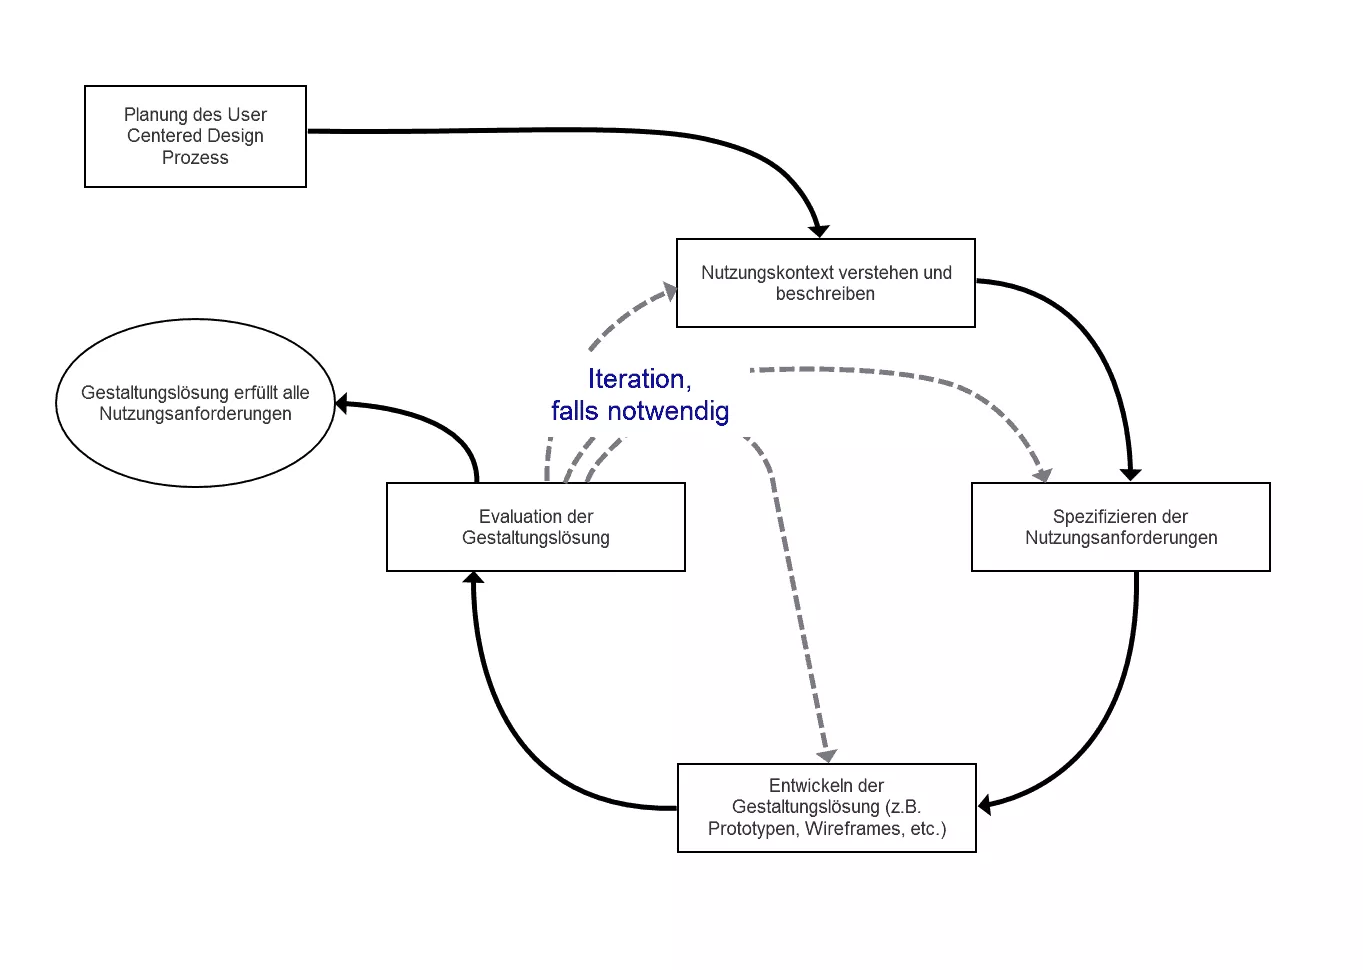
\includegraphics[width=.75\linewidth]{thesis/images/Frieling_UCD-Prozess.png}
    \caption[Ablauf des User-Centered Design Prozesses]{Ablauf des User-Centered Design Prozesses \cite{frieling_user_2019}}
    \label{fig:ucd-prozess-ablauf}
\end{figure}

\subsection{Prinzipien \& Phasen}
\label{sub-sec:prinzipien-phasen-ucd}

In Abschnitt \ref{sec:überblick-ucd} ab Seite \pageref{sec:überblick-ucd} findet sich ein grober Überblick darüber, was genau \acl{ucd} ist und wie der Ablauf aussieht beziehungsweise aussehen könnte. Anhand der genannten Informationen und Herangehensweise können die Prinzipien und Phasen des \ac{ucd} jedoch noch einmal detaillierter beschrieben werden.

Frieling beschreibt in \cite{frieling_user_2019}, dass der angesprochene iterative Prozess aus insgesamt vier Schritten (exklusive etwaiger Iterationen) besteht, welche auch in Abbildung \ref{fig:ucd-prozess-ablauf} auf Seite \pageref{fig:ucd-prozess-ablauf} zu finden sind:
\begin{itemize}
    \item Analyse der Nutzerkontexte
    \item Definition konkreter Anforderungen
    \item Entwicklung eines Konzeptes und Prototyps
    \item Evaluation und Testung
\end{itemize}

Frieling unterteilt diese vier Phasen in Abbildung \ref{fig:ucd-prozess-teildisziplinen} auf Seite \pageref{fig:ucd-prozess-teildisziplinen} noch einmal in drei Teildisziplinen: dem \enquote{User Requirements Engineering}, dem \enquote{Konzept} und der \enquote{User Research}.

\begin{figure}[ht!]
    \centering
    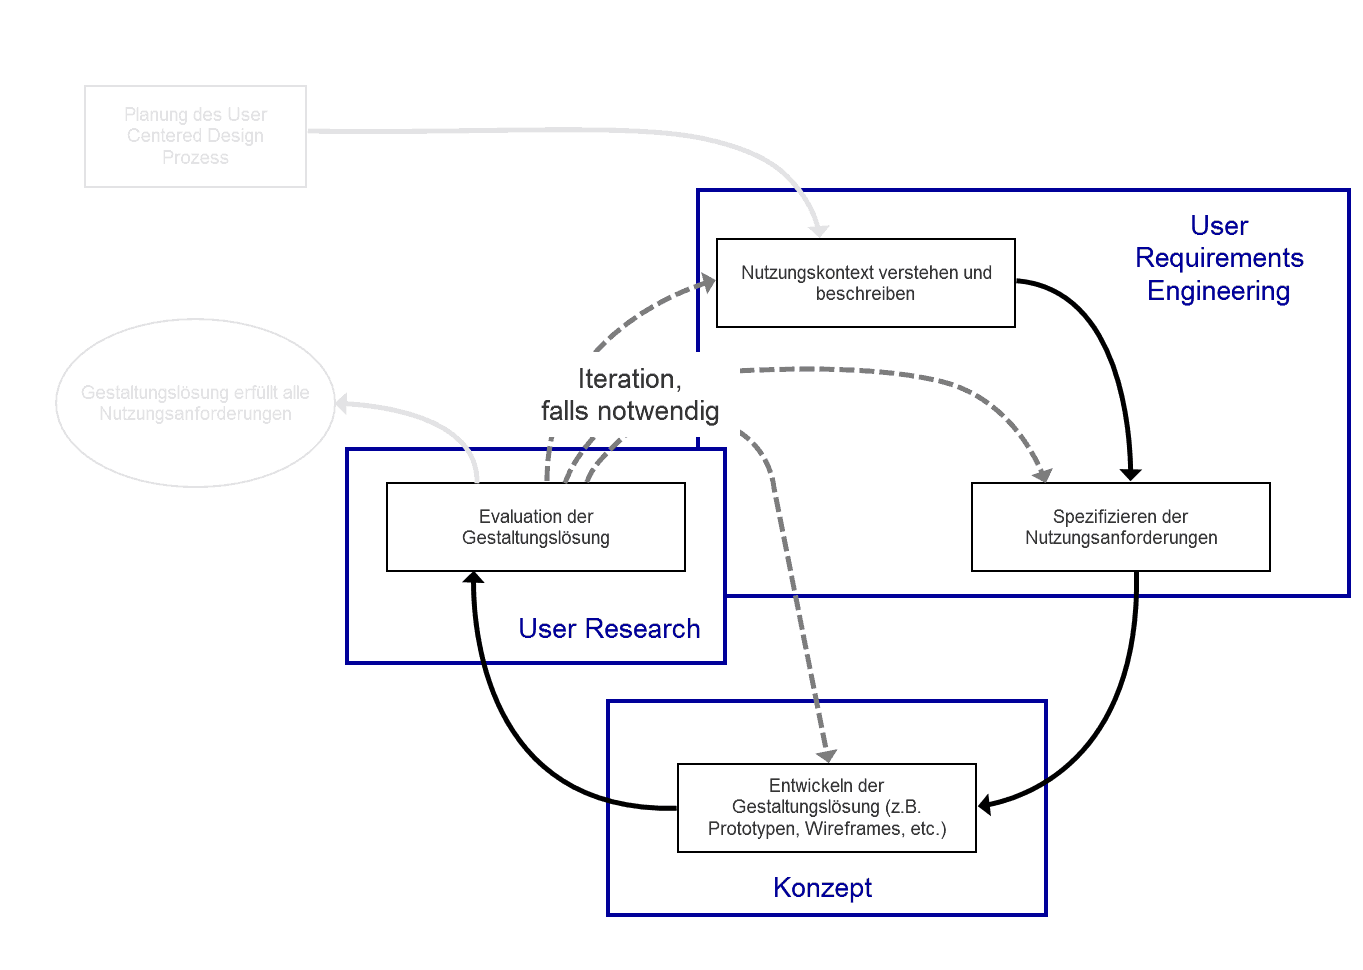
\includegraphics[width=.75\linewidth]{thesis/images/Frieling_UCD-Prozess-Teildisziplinen.png}
    \caption[User-Centered Design Prozesses aufgeteilt in drei Teildisziplinen]{User-Centered Design Prozesses aufgeteilt in drei Teildisziplinen \cite{frieling_user_2019}}
    \label{fig:ucd-prozess-teildisziplinen}
\end{figure}

\subsubsection*{User Requirements Engineering}
\label{sub-sub-sec:user-requirements-engineering}
Beim Requirements Engineering geht es um das bestmögliche Verständnis des jeweiligen Kontexts der Nutzer:innen, welches sowohl Aufgaben, zu Verfügung stehende Ressourcen sowie die Umgebung, in der das Produkt oder die Software genutzt wird, umfasst. \cite{frieling_user_2019}

\medskip

Durch die Definition und Ausarbeitung von Nutzergruppen können direkte und indirekte Nutzer:innen unterschieden werden. Direkte User:innen interagieren direkt mit dem System, während indirekte User:innen mit den Ergebnissen des Systems arbeiten. Die Analyse hilft dabei, relevante Merkmale der Anwender:innen zu identifizieren und auf dieser Grundlage beispielsweise Personas zu erstellen. Diese Personas sind fiktive Personen, die jedoch auf den gesammelten Informationen und Merkmalen basieren. Sie dienen dazu, ein besseres Verständnis für die Bedürfnisse und möglichen Anforderungen der User:innen zu entwickeln und um dieses schlussendlich während der weiteren Entwicklung einsetzen zu können. \cite{frieling_user_2019}

\medskip

Neben den jeweiligen Nutzergruppen und Personas sind auch die verfügbaren Ressourcen und die Umgebung, in der ein Produkt oder eine Software genutzt wird, von großer Bedeutung. Zeit, technische Ressourcen und die Geduld der Anwender:innen spielen eine wichtige Rolle und beeinflussen die Anforderungen an ein System. Zusätzlich haben die soziale, technische und psychische Umgebung einen Einfluss auf die Reaktionen und Wahrnehmung der Nutzer:innen bei der Durchführung von Aufgaben und Tätigkeiten und dürfen daher nicht außer Acht gelassen werden. \cite{frieling_user_2019}

\subsubsection*{Konzept}
\label{sub-sub-sec:konzept}

Nach der entsprechenden Umsetzung und Analyse des Requirements Engineering fokussiert sich die nächste Phase laut \cite{frieling_user_2019} auf die Ausarbeitung und Umsetzung eines Konzeptes sowie eines Prototyps anhand der ausgearbeiteten Anforderungen. Dabei sollten, je nach Art des Vorhabens, die unterschiedlichen Teams und Fachbereiche an einer gemeinsamen Ausarbeitung beteiligt sein. Neben der Ausarbeitung eines Konzeptes kann parallel dazu auch bereits die erste Ausarbeitung eines Prototyps erfolgen, um frühzeitig auf technische Limitierungen und daraus entstehende Ideen reagieren zu können. \cite{frieling_user_2019}

\subsubsection*{User Research}
\label{sub-sub-sec:user-research}

Als \enquote{letzte} Phase im iterativen Prozess definiert Frieling in \cite{frieling_user_2019} die Evaluation des umgesetzten Systems, Produkts oder der Software. Das Ziel der Evaluation besteht darin, Erkenntnisse zu gewinnen und die Entwicklung zu kontrollieren. Während der Entwicklung kann eine formative Evaluation durchgeführt werden, bei der Hypothesen getestet werden, um weitere oder neue Erkenntnisse zu gewinnen. Eine summative Evaluation findet am Ende der Entwicklung statt und dient oft zur abschließenden Abnahme einer Version oder eines Projektzwischenstandes. Die Art der Evaluation hängt vom Projekt und den spezifischen Anforderungen ab, wobei Usability-Tests oder andere Verfahren in der Softwareentwicklung häufig verwendet werden. \cite{frieling_user_2019}

\section{Unterschied zwischen User- und Human-Centered Design}
\label{sec:unterschied-ucd-hcd}

Im Zuge der Recherche zum \acl{ucd} ist oftmals auch der Begriff des \ac{hcd} zur Sprache gekommen. Obwohl die Unterscheidung zwischen den beiden Konzepten je nach Auslegung sehr subtil ausfällt, ist sie dennoch klar erkennbar und kann benannt werden.

\medskip

\cite{ionos_se_user-centered_2022} beschreibt den Unterschied darin, dass sich das \ac{ucd} auf eine spezifische Gruppe an Anwender:innen fokussiert, während beim \ac{hcd} nicht nur die konkreten Nutzer:innen selbst, sondern auch anderweitige Stakeholder betrachtet und in den beschriebenen Prozess und die Entwicklung mit eingebunden werden.

\medskip

Weimer stellt den Unterschied zwischen den beiden Ansätzen klarer dar: Während das \ac{hcd} die Zielgruppe in der gesamten Menschheit sieht und sich bei der Entwicklung von Konzepten, Prototypen und Lösungen vorrangig auf universelle Prinzipien aus Psychologie, Soziologie, Anthropologie und anderen Wissenschaften stützt, um menschliche Bedürfnisse zu priorisieren, verfolgt das \ac{ucd} einen fokussierteren Ansatz. Der \ac{ucd}-Ansatz richtet die Aufmerksamkeit auf spezifische Gruppen von Menschen, sprich Nutzer:innen, die durch gemeinsame Eigenschaften, Fähigkeiten sowie vor allem durch gemeinsame Aufgaben und Ziele verbunden sind. Bei der Anwendung greift der \ac{ucd}-Ansatz meist auch auf die Methoden des \ac{hcd} zurück. \cite{weimer_difference_2022}

\section{Verknüpfung mit dieser Arbeit}
\label{sec:ucd-verknüpfung-arbeit}

Die nachfolgenden Kapitel dieser Arbeit behandeln verschiedene Themenbereiche und Schwerpunkte. Neben der Analyse des bestehenden Systems wird, unter anderem, die angewandte Forschungsethik der \acl{fek} der \acl{fhv} genauer betrachtet und es werden Anforderungen an ein neues System definiert.

Tabelle \ref{tab:zurordnung-kapitel-ucd} auf Seite \pageref{tab:zurordnung-kapitel-ucd} gibt einen Ausblick auf die kommenden Kapitel und zeigt zeitgleich auf, dass die Kapitel dieser Arbeit (mit der bewussten Ausnahme des Kapitel \ref{chap:einleitung} -- \nameref{chap:einleitung}) einer der Phasen des \acl{ucd} zugeordnet werden können, da im Rahmen der Vorbereitung dieser Mastearbeit wurde gezielt darauf geachtet, den allgemeinen Aufbau dem des \ac{ucd} anzupassen.

\begin{table}[ht]
    \centering
    \begin{tabular}{p{.35\linewidth} | p{.55\linewidth}}
        \textbf{Phase} & \textbf{Kapitel} \\ \hline
        \multirow{3}{\linewidth}{Analyse des Nutzerkontextes} & Kapitel \ref{chap:kriterien-forschungsethik} -- \nameref{chap:kriterien-forschungsethik} \\ \cline{2-2} 
         & Kapitel \ref{chap:analyse-bestehendes-system-prozess} -- \nameref{chap:analyse-bestehendes-system-prozess} \\ \cline{2-2} 
         & Kapitel \ref{chap:analyse-anderer-prozesse} -- \nameref{chap:analyse-anderer-prozesse} \\ \hline
        Definition konkreter Anforderungen & Kapitel \ref{chap:anforderung-neues-system} -- \nameref{chap:anforderung-neues-system} \\ \hline
        Entwicklung eines Konzeptes und Prototyps & \ref{chap:ausarbeitung-umsetzung-prototyp} -- \nameref{chap:ausarbeitung-umsetzung-prototyp} \\ \hline
        Evaluation und Testung & \colorbox{yellow}{Kapitel 8}
    \end{tabular}
    \caption{Zuordnung der Kapitel dieser Masterarbeit zu den Phasen des \acl{ucd}}
    \label{tab:zurordnung-kapitel-ucd}
\end{table}

\subsubsection*{Anmerkung}
\label{sub-sub-sec:ucd-verknüpfung-anmerkung}

Die Ausarbeitung von Nutzerkontexten und Personas, wie in Abschnitt \ref{sub-sec:prinzipien-phasen-ucd} ab Seite \pageref{sub-sec:prinzipien-phasen-ucd} erwähnt, wurde aufgrund des begrenzten Rahmens dieser Masterarbeit und der zeitlichen Beschränkungen ausgelassen. Aufgrund der ersten Problemanalyse und Fragestellung, die in Kapitel \ref{chap:einleitung} ab Seite \pageref{chap:einleitung} durchgeführt wurde, können die Anwender:innen jedoch einer eng definierten Gruppe von Mitarbeitenden der \ac{fhv} zugeordnet werden, deren Kontexte sich den Interviews entnehmen lassen.

Sollte der entwickelte Prototyp und das System außerhalb der \acl{fhv} verwendet werden und weitere Funktionalitäten und Arbeitsprozesse abdecken müssen, würde es Sinn machen, eine detaillierte Ausarbeitung der Nutzerkontexte sowie Personas und eine erneute Analyse der Anforderungen durchzuführen.

\chapter{Kriterien der Forschungsethik}
\label{chap:kriterien-forschungsethik}

Wie bereits in Abschnitt \ref{sec:motivation} ab Seite \pageref{chap:einleitung} angesprochen, behandelt die \acl{fek} der \acl{fhv} auf Antrag wissenschaftliche Untersuchungen, bei denen an oder mit Menschen geforscht wird oder die Auswirkungen auf Menschen haben können. \cite{fachhochschule_vorarlberg_gmbh_forschungsethik-kommission_2021} Für die Bewertung von Forschungsprojekten und Entwicklungsarbeiten und Erstellung eines Votums im Rahmen eines Ethikantrages kommen dabei unterschiedliche Grundsätze, Leitbilder und Kriterien zum Einsatz, auf die im Folgenden genauer eingegangen wird.

\section{Grundsätze, Leitbilder \& Wertekomplexe}
\label{sec:grundsätze-leitbilder-wertekomplexe}

Die \ac{fek} gibt in ihrer Satzung \cite[1]{forschungsethik-kommission_der_fachhochschule_vorarlberg_satzung_2021} sowie ihrer Verfahrensordnung \cite[1\psq]{forschungsethik-kommission_der_fachhochschule_vorarlberg_verfahrensordnung_2020} an, nach welchen Grundsätzen, Leitbildern und Wertekomplexen ethische Fragen und Themenstellungen behandelt werden. Dazu zählen:
\begin{itemize}
    \item der Wertekatalog der \acl{fhv} \cite{kollegium_der_fachhochschule_vorarlberg_gmbh_wertekatalog_2022},
    \item die Empfehlungen der Deutschen Gesellschaft für Psychologie für Forschende und Ethikkommissionen \cite{deutsche_gesellschaft_fur_psychologie_ev_ethisches_2018},
    \item die Grundwerte der Europäischen Union im Vertrag über die Europäische Union,
    \item die Datenschutz-Grundverordnung der Europäischen Union,
    \item den \enquote{Meta-Code of Ethics} der European Federation of Psychologists' Associations \cite{european_federation_of_psychologists_associations_meta-code_2005},
    \item die Deklaration von Helsinki des Weltärztebundes \cite{world_medical_association_world_2013} sowie
    \item den \enquote{Code of Ethics for Health Information Professionals} der International Medical Informatics Association \cite{international_medical_informatics_association_imia_2016}
\end{itemize}

Bei der Beurteilung eines Ethikantrages wird, unter Zuhilfenahme der genannten Dokumente und Leitlinien, vor allem geprüft, ob ein vertretbares Verhältnis zwischen dem zu erwartenden Nutzen und den mit der Forschung verbundenen Risiken besteht, ob identifizierte Risiken so gering wie möglich gehalten werden und ob eine ausreichende Einwilligung etwaiger Proband:innen sichergestellt ist. Ebenso werden eingereichte Ethikanträge dahingehend geprüft, ob Angaben zu beispielsweise der geplanten Stichprobe, der Zielgruppen, der Aufklärung von betroffenen Personen und Angaben zu den Rechten für Betroffene in korrekter Weise gemacht und geplant wurden. \cite[1\psq]{forschungsethik-kommission_der_fachhochschule_vorarlberg_verfahrensordnung_2020}

Teilaspekte, die den Datenschutz oder das Forschungsdesign sowie die Forschungsqualität betreffen, werden von der \ac{fek} auch außerhalb des konkreten Rahmens der ethischen Beurteilung betrachtet. Grobe Fehler und allgemeines Feedback werden im angefertigten Protokoll, welches Antragsteller:innen nach abschließendem Votum übermittelt wird, mitgeteilt, um das potenzielle Vergeuden von (Zeit-)Ressourcen zu vermeiden und auf Fehler sowie Bedenken der Kommission hinweisen zu können.\footnote{Um ein konkretes Beispiel dafür zu nennen: In der ursprünglichen Planung für diese Masterarbeit war ein Fragebogen vorgesehen, der sowohl an Master-Studierende als auch Forschungsmitarbeitende der \ac{fhv} ausgesendet werden sollte (siehe dazu Anhang \ref{appendix:eingereichter-ethikantrag} ab Seite \pageref{appendix:eingereichter-ethikantrag}). Nach entsprechender Rückmeldung der \ac{fek} (siehe dazu Anhang \ref{appendix:rückmeldung-fek} ab Seite \pageref{appendix:rückmeldung-fek}) wurde diese Idee jedoch weitestgehend verworfen.\label{footnote:ursprüngliche-planung-leitfaden}} \cite[1\psq]{forschungsethik-kommission_der_fachhochschule_vorarlberg_verfahrensordnung_2020}

\medskip

Abseits von den in der Satzung und Verfahrensordnung definierten Leitlinien und Kriterien sieht die \ac{fek} ihre Aufgabe ebenso darin (siehe dazu Anhang \ref{appendix:gruppendiskussion} ab Seite \pageref{appendix:gruppendiskussion}), Forschenden die Möglichkeit zu bieten, die Qualität ihres Forschungsvorhabens durch externe, nicht involvierte Personen betrachten und bewerten zu lassen. Sowohl aus der eigenen Motivation der Forschenden heraus, Feedback zu erhalten, als auch aufgrund von externen Anforderung, denen die Forschungsvorhaben unterliegen (wie beispielsweise bei der Veröffentlichung in einem wisschenschaftlichen Journal). Die Mitglieder der \ac{fek} empfinden die ethische Bewertung dabei als \enquote{Korrektivfunktion} sowie \enquote{Qualitätsmodell}, was in sehr ähnlicher Form auch in einem der Interviews mit einem Forschenden der \ac{fhv} so wahrgenommen wurde (siehe dazu Anhang \ref{appendix:interview-1} ab Seite \pageref{appendix:interview-1}).

\section{Angewandter Kriterienkatalog}
\label{sec:angewandter-kriterienkatalog}

Die schlussendlich durchgeführte Begutachtung eines Ethikantrages und der damit verbundenen Forschungsarbeit wird Antragsteller:innen in Form einer schriftlichen Entscheidung beziehungsweise Stellungnahme übermittelt. \cite[4]{forschungsethik-kommission_der_fachhochschule_vorarlberg_verfahrensordnung_2020} Wie in Anhang \ref{appendix:rückmeldung-fek} ab Seite \pageref{appendix:rückmeldung-fek} ersichtlich ist, ist diese Rückmeldung in einen schriftlichen Teil mit Hinweisen und Anmerkungen sowie einen Teil mit der jeweiligen Bewertung der einzelnen Kriterien des Kriterienkataloges aufgeteilt.

Die einzelnen Bewertungskriterien orientieren sich dabei an unterschiedlichen Quellen (unter anderem \cite{manzeschke_meestar_2015, marckmann_was_2000, schuchter_care_2018}) und decken Gesichtspunkte von der menschlichen Interaktion auf Augenhöhe über die technische Datenspeicherung in anonymisierter Form oder der Auslegung des sozialen Settings bis hin zur Forschungsintegrität ab. Eine darauf aufbauende Beurteilung der Kriterien findet in einem dreistufigen System statt, bei dem unterschieden wird, ob ethische Unbedenklichkeit (\enquote{Stufe I}) herrscht, Maßnahmen ergriffen werden müssen, um ethische Unbedenklichkeit (\enquote{Stufe II}) gewährleisten zu können oder ob einzelne Gesichtspunkte als ethisch bedenklich (\enquote{Stufe III}) einzustufen sind. \cite[1]{forschungsethik-kommission_der_fachhochschule_vorarlberg_kriterienkatalog_2021}

\medskip

In manchen Fällen, wie auch bei der erhaltenen Rückmeldung zum Ethikantrag dieser Masterarbeit (siehe Anhang \ref{appendix:rückmeldung-fek} ab Seite \pageref{appendix:rückmeldung-fek}), kann es vorkommen, dass die gefällte Bewertung im dreistufigen System nicht eindeutig die Meinung der Kommission beziehungsweise der einzelnen Mitglieder widerspiegeln kann. Im angesprochenen Anhang ist ersichtlich, dass zwei Bewertungskriterien sowohl mit \enquote{Stufe I} als auch mit \enquote{Stufe II} bewertet wurden. Die \ac{fek} erklärt (siehe Anhang \ref{appendix:gruppendiskussion} ab Seite \pageref{appendix:gruppendiskussion}), dass es auf Grundlage des Diskurses zwar zu einer schlussendlichen Bewertung gekommen ist, es dennoch unterschiedliche Meinungen, Einschätzungen und auch Bedenken der einzelnen Mitglieder gegeben hat, die entsprechend kommuniziert und nicht komplett außen vor gelassen werden.

\medskip

Vier der sieben angewandten Bewertungskriterien der \ac{fek} lassen sich bei genauerer Betrachtung den Thesen von Beauchamp und Childress zuordnen, die in \cite{beauchamp_principles_1994} vier moralische Prinzipien definiert haben. Auch die im Kriterienkatalog genannten Quellen (siehe \cite[2]{forschungsethik-kommission_der_fachhochschule_vorarlberg_kriterienkatalog_2021}) beziehen sich stellenweise explizit darauf\footnote{Sowohl \cite{marckmann_was_2000} als auch \cite{schuchter_care_2018} nennen die vier moralischen Prinzipien explizit in ihren Arbeiten.}:
\begin{itemize}
    \item Kriterium \enquote{Autonomie} in Anlehnung an Beauchamp's und Childress' \enquote{Respect for Autonomy} \cite[101-149]{beauchamp_principles_1994}
    \item Kriterium \enquote{Fürsorge} in Anlehnung an Beauchamp's und Childress' \enquote{Beneficence} \cite[202-248]{beauchamp_principles_1994}
    \item Kriterium \enquote{Gerechtigkeit} in Anlehnung an an Beauchamp's und Childress' \enquote{Justice} \cite[249-301]{beauchamp_principles_1994}
    \item Kriterium \enquote{Menschliche Sicherheit} im allgemeineren Sinne in Anlehnung an Beauchamp's und Childress' \enquote{Nonmaleficience} \cite[150-201]{beauchamp_principles_1994}
\end{itemize}

In der Gruppendiskussion (siehe Anhang \ref{appendix:gruppendiskussion} ab Seite \pageref{appendix:gruppendiskussion}) erwähnt die \acl{fek}, dass die Auslegung der Kriterien nicht immer strikt erfolgt und für gewisse Anträge und Forschungsprojekte angepasst werden kann und muss. Bei Bedarf reichen beispielsweise nur sechs Kriterien als Bewertungsgrundlage aus, während die bereits angesprochene Beurteilung des Forschungs-Designs mit entsprechendem Feedback de facto als achtes, informelles Kriterium gehandhabt wird.

Laut Aussage der Kommission sind die Kriterien ebenso Grundlage dafür, um eingereichte Ethikanträge ohne jegliches ethisches Votum an die Antragsstellenden zu retournieren, wenn das Forschungsvorhaben oder die mit dem Antrag verbundene Arbeit keinerlei ethischen Implikationen mit sich bringt.

\chapter{Analyse des bestehenden Systems \& Prozesses}
\label{chap:analyse-bestehendes-system-prozess}

Die in Kapitel \ref{chap:kriterien-forschungsethik} ab Seite \pageref{chap:kriterien-forschungsethik} dargelegten Leitsätze und Kriterien der Forschungsethik bilden den Grundstein für die Arbeit der \acl{fek} an der \acl{fhv}. Damit Forschende und Master-Studierende eine ethische Beurteilung ihrer Arbeit in Form eines Votums erhalten können, müssen verschiedene Schritte durchlaufen, Angaben gemacht und Dokumente ausgefüllt werden, die im Prozess eines Ethikantrages benötigt werden.

\medskip

Das nachfolgende Kapitel fokussiert sich in der Analyse zuerst auf die Sichtweise aus der \enquote{Vogelperspektive}, bevor die einzelnen Prozess-Schritte aus der Sicht von Antragsteller:innen und der Sicht der \ac{fek} genauer beleuchtet und die Word"=Antragsvorlage sowie die bestehenden Stärken und Probleme im Detail skizziert werden.

\section{Ablauf eines Ethikantrages}
\label{sec:ablauf-ethikantrag}

Der Ablauf eines Ethikantrages kann in die folgenden zehn Schritte unterteilt werden (\cite{fachhochschule_vorarlberg_gmbh_forschungsethik-kommission_2021, forschungsethik-kommission_der_fachhochschule_vorarlberg_verfahrensordnung_2020} sowie Anhang \ref{appendix:gruppendiskussion} ab Seite \pageref{appendix:gruppendiskussion}):

\begin{itemize}
    \item \textbf{Schritt 1:} Herunterladen der Antragsvorlage in Form einer Word"=Antragsvorlage durch den:die Antragsteller:in
    \item \textbf{Schritt 2:} Ausfüllen der Antragsvorlage durch den:die Antragsteller:in
    \item \textbf{Schritt 3:} Übermittlung des ausgefüllten Antrages sowie allfälliger Anlagen an den:die Vorsitzende:n der Kommission durch den:die Antragsteller:in
    \item \textbf{Schritt 4:} Formale Überprüfung auf Antragsberechtigung und Vollständigkeit durch den:die Vorsitzende:n der \ac{fek}
    \item \textbf{Schritt 5:} Rückmeldung an Antragsteller:in sowie Weiterleitung der Unterlagen an stimmberechtigte Mitglieder der \ac{fek} durch den:die Vorsitzende:n
    \item \textbf{Schritt 6:} Individuelle Begutachtung der eingereichten Unterlagen durch die stimmberechtigten Mitglieder der \ac{fek}
    \item \textbf{Schritt 7:} Diskussion und Bewertung der eingereichten Unterlagen in der nächsten Sitzung der \ac{fek} durch die stimmberechtigten Mitglieder
    \item \textbf{Schritt 8:} Anfertigung des Protokolls sowie des Votums und Aussendung dieser vorläufigen Stellungnahme an die stimmberechtigten Mitglieder durch den:die Vorsitzende:n der \ac{fek}
    \item \textbf{Schritt 9:} Begutachtung der vorläufigen Stellungnahme und Rückmeldung von Feedback an den:die Vorsitzende:n der \ac{fek} durch die stimmberechtigten Mitglieder
    \item \textbf{Schritt 10:} Einarbeitung von eingegangenem Feedback der stimmberechtigten Mitglieder und finale Aussendung des Votums beziehungsweise der ethischen Stellungnahme an die antragsstellende Person durch den:die Vorsitzende:n der \ac{fek}
\end{itemize}

Bei Bedarf weiten sich die aufgezählten Schritte aus, wenn von der \ac{fek} festgestellt wird, dass die eingereichten Unterlagen entweder nicht vollständig sind oder Informationen fehlen, sodass das Nachliefern von Informationen oder eine erneute Einreichung notwendig ist.

\subsection{Sicht der Antragsteller:innen}
\label{sub-sec:ablauf-sicht-Antragsteller}

Der grundlegende Ablauf und der Prozess eines Ethikantrages kann von potenziellen Antragsstellenden sowohl auf der Website der \ac{fhv} auf der Unterseite der \ac{fek} (\cite{fachhochschule_vorarlberg_gmbh_forschungsethik-kommission_2021}) als auch in der öffentlich einsehbaren Verfahrensordnung (\cite{forschungsethik-kommission_der_fachhochschule_vorarlberg_verfahrensordnung_2020}) der Kommission in vollem Detail nachvollzogen werden.

Interviewpartner:in A und Interviewpartner:in B haben in den Einzelinterviews (siehe Anhang \ref{appendix:interview-1} ab Seite \pageref{appendix:interview-1} und Anhang \ref{appendix:interview-2} ab Seite \pageref{appendix:interview-2}) jeweils angegeben beziehungsweise bestätigt, dass der gesamte Prozess und auch die für sie notwendigen Schritte klar und nachvollziehbar waren, um ein Votum der Kommission erhalten zu können.

\medskip

Die in Abschnitt \ref{sec:ablauf-ethikantrag} ab Seite \ref{sec:ablauf-ethikantrag} aufgezählten Punkte umfassen dabei zumindest drei Schritte, die die Antragsstellenden konkret betreffen und von ihnen maßgeblich umgesetzt werden müssen:
\begin{itemize}
    \item \textit{Schritt 1} mit dem Ausfindigmachen und Herunterladen der Antragsvorlage in Form der Word"=Antragsvorlage,
    \item \textit{Schritt 2} mit dem Ausfüllen und Ausarbeiten der im Antrag gestellten Fragen sowie
    \item \textit{Schritt 3} mit der Übermittlung des Antrages sowie allfälliger Anlagen an die \ac{fek}
\end{itemize}

\noindent\textit{Schritt 5} und \textit{Schritt 10} betreffen die Antragsteller:innen insoweit ebenso, als dass sie dort Informationen zum weiteren Vorgehen beziehungsweise das finale Votum erhalten.

Ein Punkt, der in der Auflistung lediglich implizit angenommen wird, ist die Entscheidung zur Einreichung eines Ethikantrages und der Weg dorthin (insbesondere wenn es Unklarheiten darüber gibt, ob ein Ethikantrag überhaupt notwendig ist oder ob das Forschungsvorhaben antragsberechtigt ist). Dieser Umstand wird im weiteren Verlauf dieses Kapitels noch genauer behandelt.

\subsection{Sicht der \acl{fek}}
\label{sub-sec:ablauf-sicht-fek}

Die \acl{fek} hat den Ablauf eines Ethikantrages sowie des zugrundeliegenden Prozesses in ihrer Verfahrensordnung (\cite{forschungsethik-kommission_der_fachhochschule_vorarlberg_verfahrensordnung_2020}) sowie stichpunktartig auf der Website der \ac{fhv} auf der Unterseite der \ac{fek} (\cite{fachhochschule_vorarlberg_gmbh_forschungsethik-kommission_2021}) festgelegt und veröffentlicht.

Die in Abschnitt \ref{sec:ablauf-ethikantrag} ab Seite \pageref{sec:ablauf-ethikantrag} beschriebenen Schritte entsprechen nicht nur dem in der Verfahrensordnung theoretisch festgelegten Ablauf, sondern auch der praktischen Vorgehensweise der \ac{fek} (siehe Anhang \ref{appendix:gruppendiskussion} ab Seite \pageref{appendix:gruppendiskussion}). Die zehn identifizierten Punkte betreffen dabei zu einem Großteil die Mitglieder der Kommission direkt, wobei die Antragsteller:innen nur indirekt involviert sind:
\begin{itemize}
    \item \textit{Schritt 4} mit der Überprüfung auf Antragsberechtigung und Vollständigkeitk,
    \item \textit{Schritt 5} mit der Rückmeldung beziehungsweise Weiterleitung an alle Beteiligten,
    \item \textit{Schritt 6} mit der individuellen Begutachtung,
    \item \textit{Schritt 7} mit der gemeinsamen Diskussion und Bewertung,
    \item \textit{Schritt 8} mit der Erstellung des vorläufigen Votums,
    \item \textit{Schritt 9} mit der internen Aussendung und anschließenden Einarbeitung des erhaltenen Feedbacks sowie
    \item \textit{Schritt 10} mit der Rückmeldung an den:die Antragsstellende:n
\end{itemize}

\noindent Zusätzlich dazu werden, wie in der Gruppendiskussion (siehe Anhang \ref{appendix:gruppendiskussion} ab Seite \pageref{appendix:gruppendiskussion}) zur Sprache gekommen ist, im Vorhinein zu \textit{Schritt 3} (beziehungsweise \textit{Schritt 1} aus Sicht von Antragsteller:innen) Fragen oder Unklarheiten bei Bedarf beantwortet, ehe es zu einer Einreichung der Unterlagen und dem Start des Prozesses kommt.

\medskip

Während des Gesprächs zum Verfahrensablauf aus Sicht der Kommission (siehe Anhang \ref{appendix:gruppendiskussion} ab Seite \pageref{appendix:gruppendiskussion}) wurde der Wunsch beziehungsweise die Möglichkeit geäußert, den bestehenden Prozess für die kommende Legislaturperiode anzupassen. Aus Sicht eines Kommissions-Mitglieds wäre es möglich, das ausführliche Antragsformular durch eine schlankere Variante zu ersetzen und zusätzlich dazu ein Gespräch zwischen Antragsteller:in und Kommission im Rahmen einer Sitzung der \ac{fek} abzuhalten. Dieser Aspekt wird im Verlauf dieser Arbeit noch vertiefend aufgegriffen.

\section{Technischer Aufbau}
\label{sec:technischer-aufbau}

Der derzeitige Prozess zur Einreichung von Ethikanträgen bei der \ac{fek} an der \ac{fhv} beruht auf der Möglichkeit, im Zuge der Antragstellung eine Word"=Antragsvorlage auf Deutsch\footnote{\url{https://www.fhv.at/fileadmin/user_upload/fhv/files/forschung/Forschungsethik-Kommission/Antragsformular_EK_FHV_neu.docx} (Deutsche Version vom 06.04.2021)} oder Englisch\footnote{\url{https://www.fhv.at/fileadmin/user_upload/fhv/files/forschung/Forschungsethik-Kommission/Application_form_EK_FHV_neu.docx} (Englische Version vom 13.04.2021)} herunterzuladen, welche die benötigten Informationen von den Antragsstellenden sammelt.

Abbildung \ref{fig:dokumentenvorlage-fek} auf Seite \pageref{fig:dokumentenvorlage-fek} stellt Seite 1 der Vorlage dar, welche allgemeine Fragen zum Forschungsvorhaben enthält, sowie Seite 6, welche Fragen zum Datenschutz in Bezug auf die durchzuführende Studie oder Produktanwendung in Erfahrung bringt.

\begin{figure}[ht]
    \centering
    \begin{minipage}[t]{.49\linewidth}
        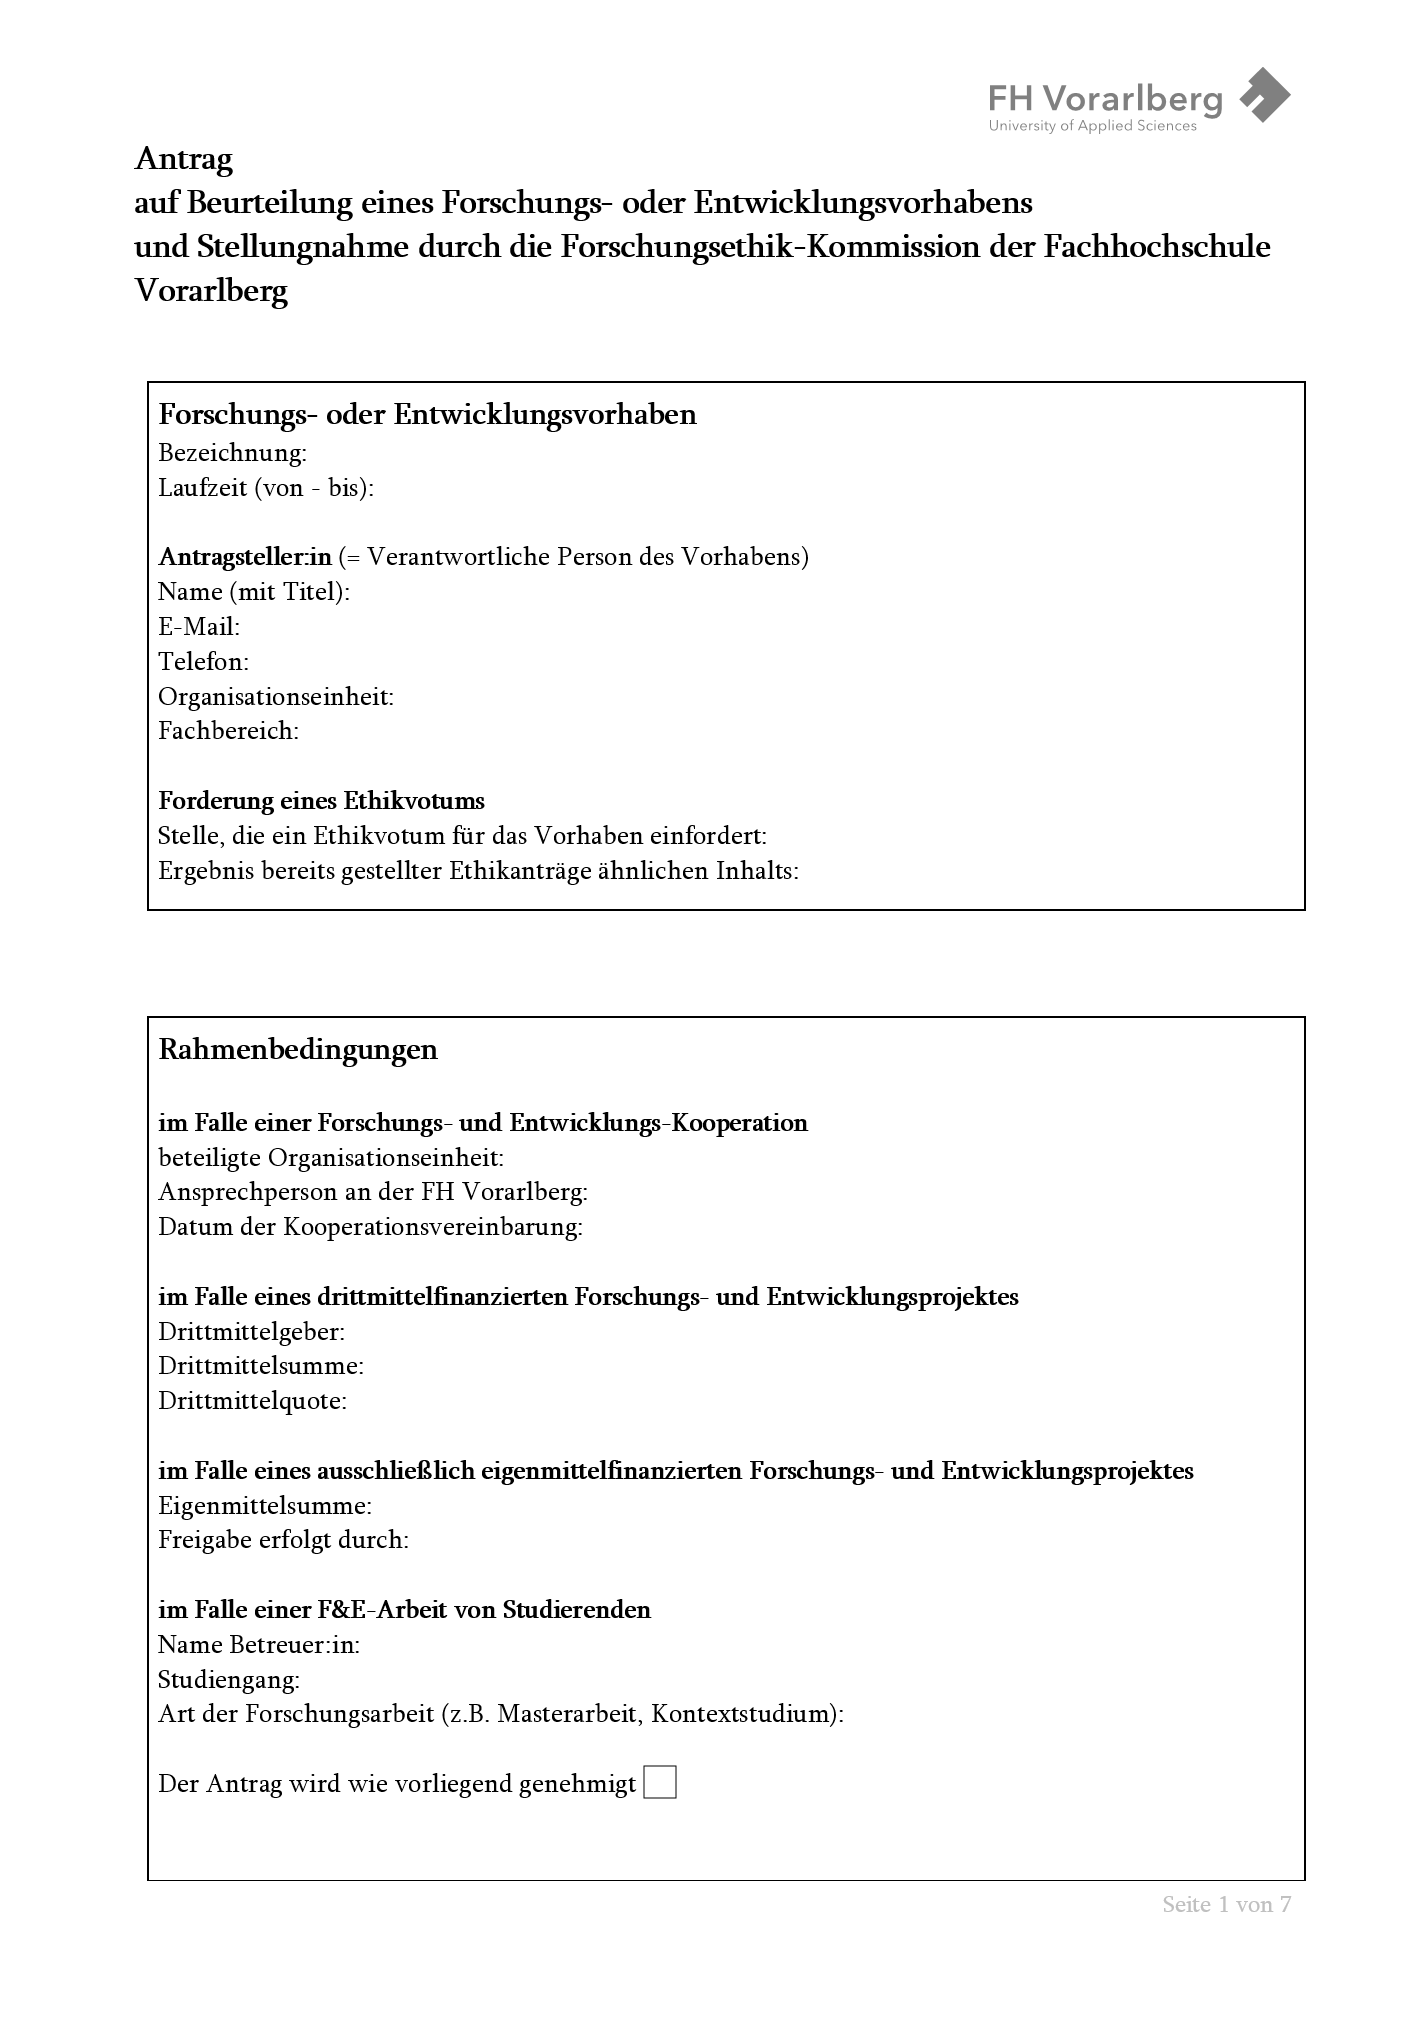
\includegraphics[width=\linewidth]{thesis/images/Luidold_Word-Vorlage-FHV-1.png}
    \end{minipage}
    \begin{minipage}[b]{.49\linewidth}
        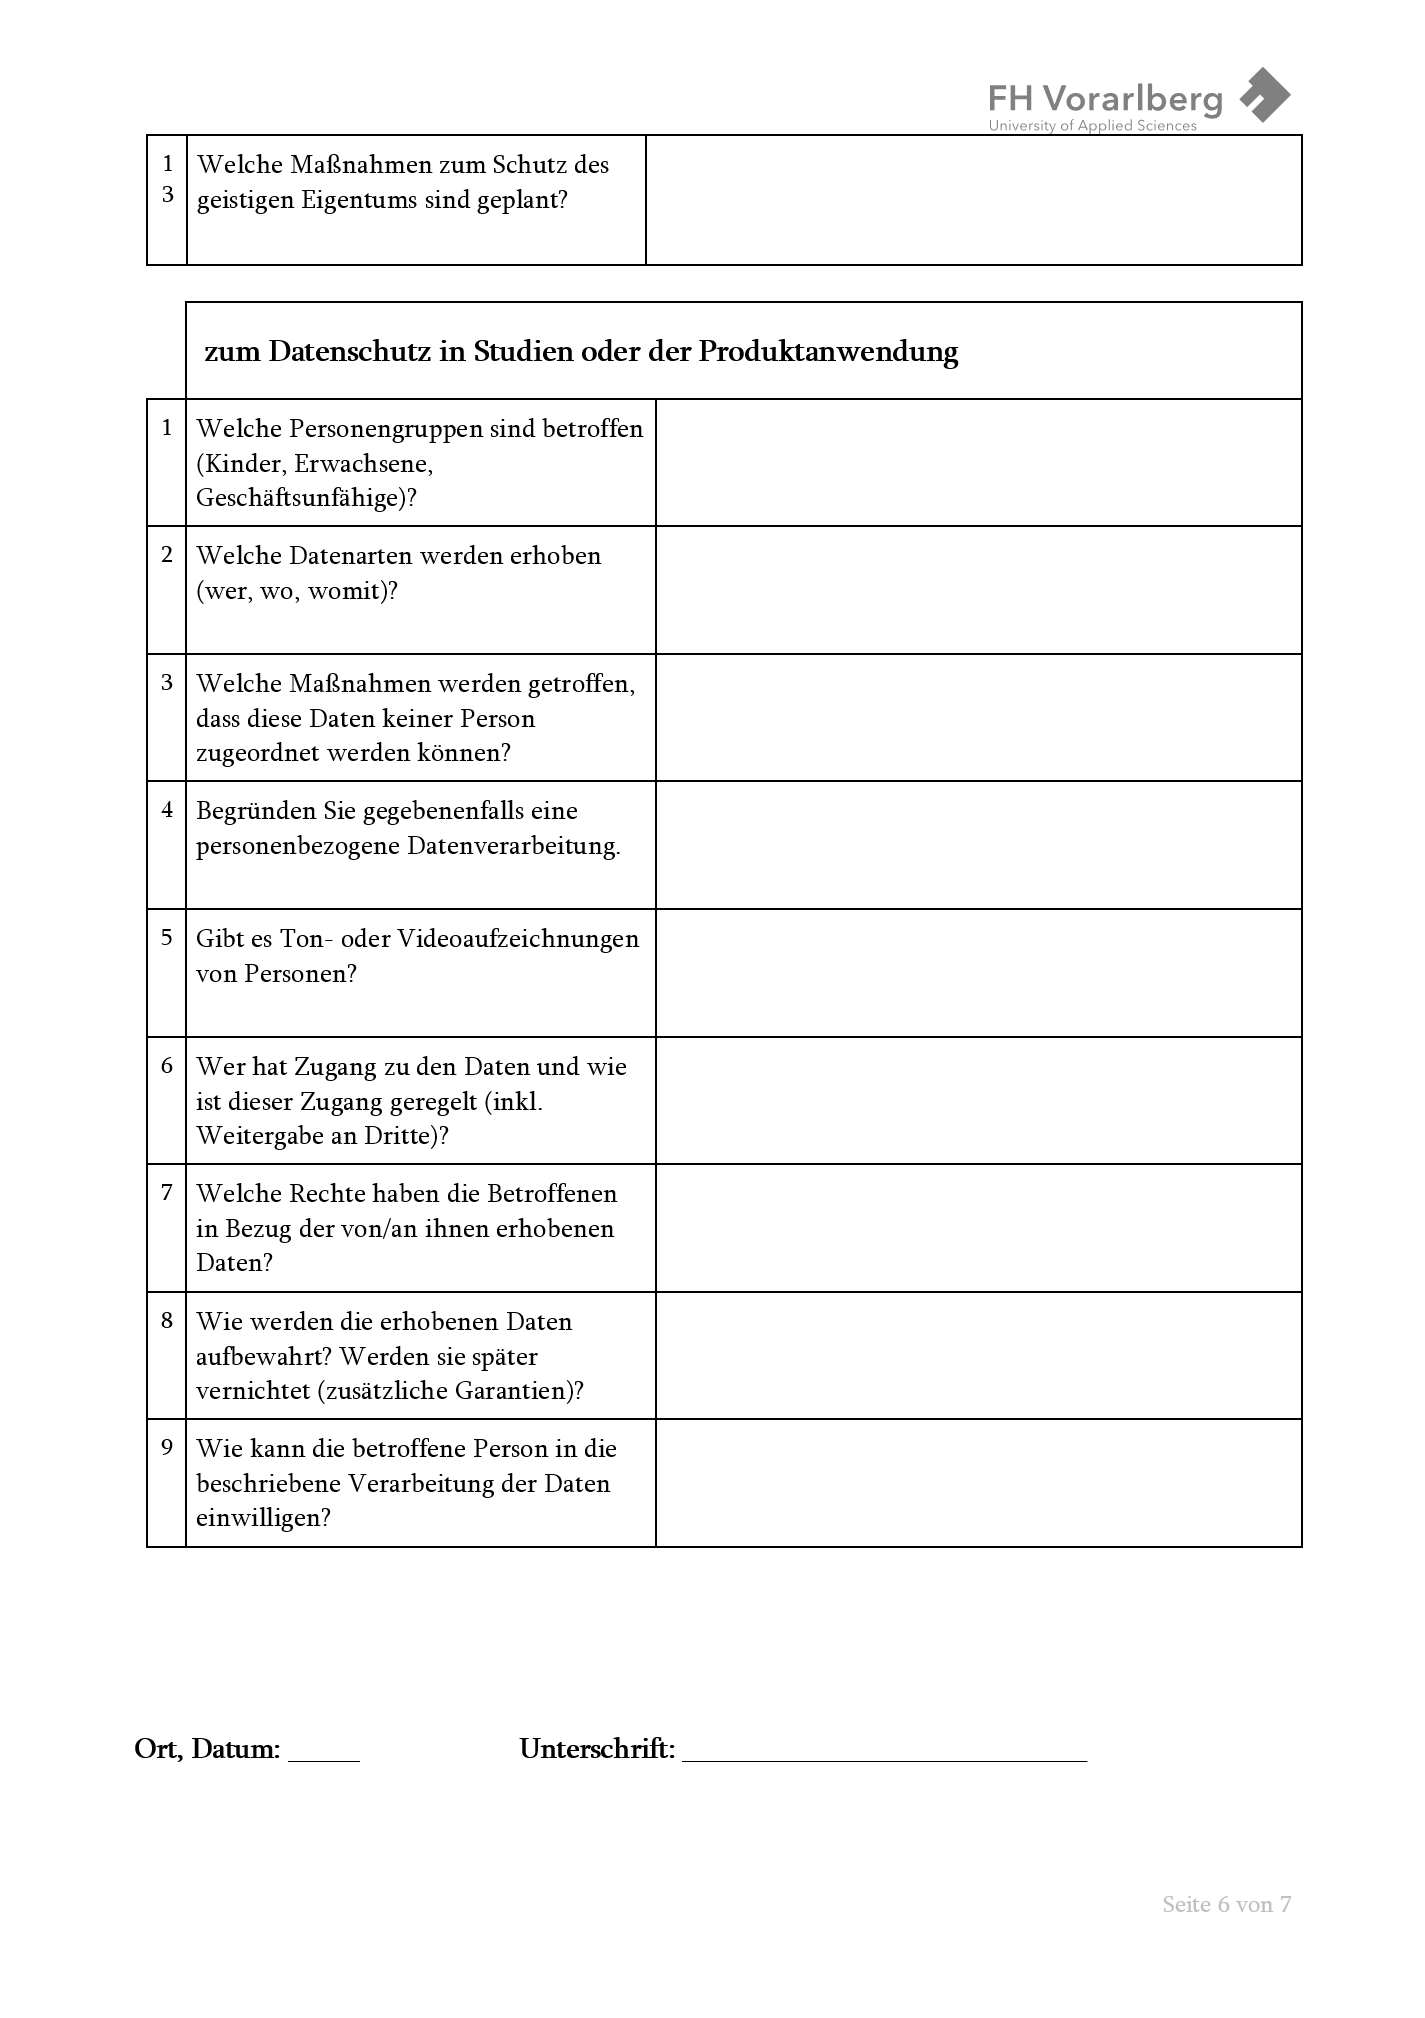
\includegraphics[width=\linewidth]{thesis/images/Luidold_Word-Vorlage-FHV-2.png}
    \end{minipage}
    \caption[{Seite 1 und Seite 6 der Word"=Antragsvorlage der \acl{fek} der \acl{fhv}}]{Seite 1 und Seite 6 der Word"=Antragsvorlage der \acs{fek} der \acs{fhv} \cite{fachhochschule_vorarlberg_gmbh_forschungsethik-kommission_2021}}
    \label{fig:dokumentenvorlage-fek}
\end{figure}

\subsection{Word"=Antragsvorlage}
\label{sub-sec:technischer-aufbau-word-antragsvorlage}

Die im \texttt{.docx}-Format zum Download angebotene Antragsvorlage beinhaltet verschiedene Abschnitte und Bereiche, in denen unterschiedliche Informationen von den Antragstellenden erhoben werden. Diese Informationen können bei der Erstellung des Ethikantrages jedoch nur in dafür vorgesehene Bereichen eingetragen werden, die auf von Microsoft Word bereitgestellten Steuerelementen basieren, ähnlich zu einem Formular. Insbesondere wird der laut \cite{ay_textfelder_2023} mittlerweile veraltete Typ \texttt{Textfeld (Formularsteuerelement)} in der gesamten Vorlage mehrfach verwendet, um das genannte Formularverhalten, in Kombination mit der von Microsoft Word bereitgestellten Funktion zur Einschränkung von Bearbeitungsmöglichkeiten, zu erzielen.

Laut Aussage der \acl{fek} (siehe Anhang \ref{appendix:gruppendiskussion} ab Seite \pageref{appendix:gruppendiskussion}) ist die Antragsvorlage auch darauf ausgelegt, hauptsächlich mit Microsoft Word editiert und ausgefüllt zu werden, da von der Kommission angenommen wird, dass Microsoft Word auf beinahe allen Systemen installiert ist.\footnote{Im Kontext der \acl{fhv} ist diese Annahme tendenziell berechtigt, da zum Zeitpunkt des Sommersemesters 2023 allen Forschenden, Lehrenden sowie Studierenden die Microsoft Office Suite im Rahmen ihrer Anstellung beziehungsweise des Studiums kostenlos zur Verfügung gestellt wird.} Die Vorlage des Antragsformulares kann unabhängig davon dennoch mit anderen \texttt{.docx}-kompatiblen Editoren (wie beispielsweise Apache Open Office\footnote{Apache Open Office (\url{https://www.openoffice.org/})}) geöffnet werden, wobei hierbei die verwendeten Formularfelder und anderweitig getroffene Einschränkungen zur Bearbeitung zur Gänze verloren gehen.

Etwaige Bedingungen, die man typischerweise in einem Formular findet (wie beispielsweise konditionale Abhängigkeiten von Eingabefeldern, die Überprüfung auf Vollständigkeit der eingegebenen Daten oder ähnliches) werden in der eingesetzten Word"=Antragsvorlage nicht verwendet beziehungsweise stehen in dieser Form gar nicht oder nur eingeschränkt zur Verfügung. Auch Formatierungsmöglichkeiten, wie beispielsweise kursiver oder unterstrichener Text oder die Nutzung von Bulletpoints, ist in den genannten Feldern dabei nicht möglich.
Abbildung \ref{fig:optionen-textformularfeld-bearbeitungsmöglichkeiten} auf Seite \pageref{fig:optionen-textformularfeld-bearbeitungsmöglichkeiten} zeigt im geöffneten Anwendungsfenster beispielhaft die Konfigurationsmöglichkeiten für die eingesetzten Formularfelder sowie auf der rechten Seite die Möglichkeit, die Dokumentenbearbeitung einzuschränken.

Als konkrete Konsequenz ergibt sich dadurch die in Abschnitt \ref{sec:ablauf-ethikantrag} ab Seite \pageref{sec:ablauf-ethikantrag} skizzierte Überprüfung auf Vollständigkeit von eingereichten Ethikanträgen, die vom Vorsitz der \ac{fek} händisch durchgeführt wird.

\begin{figure}[ht]
    \centering
    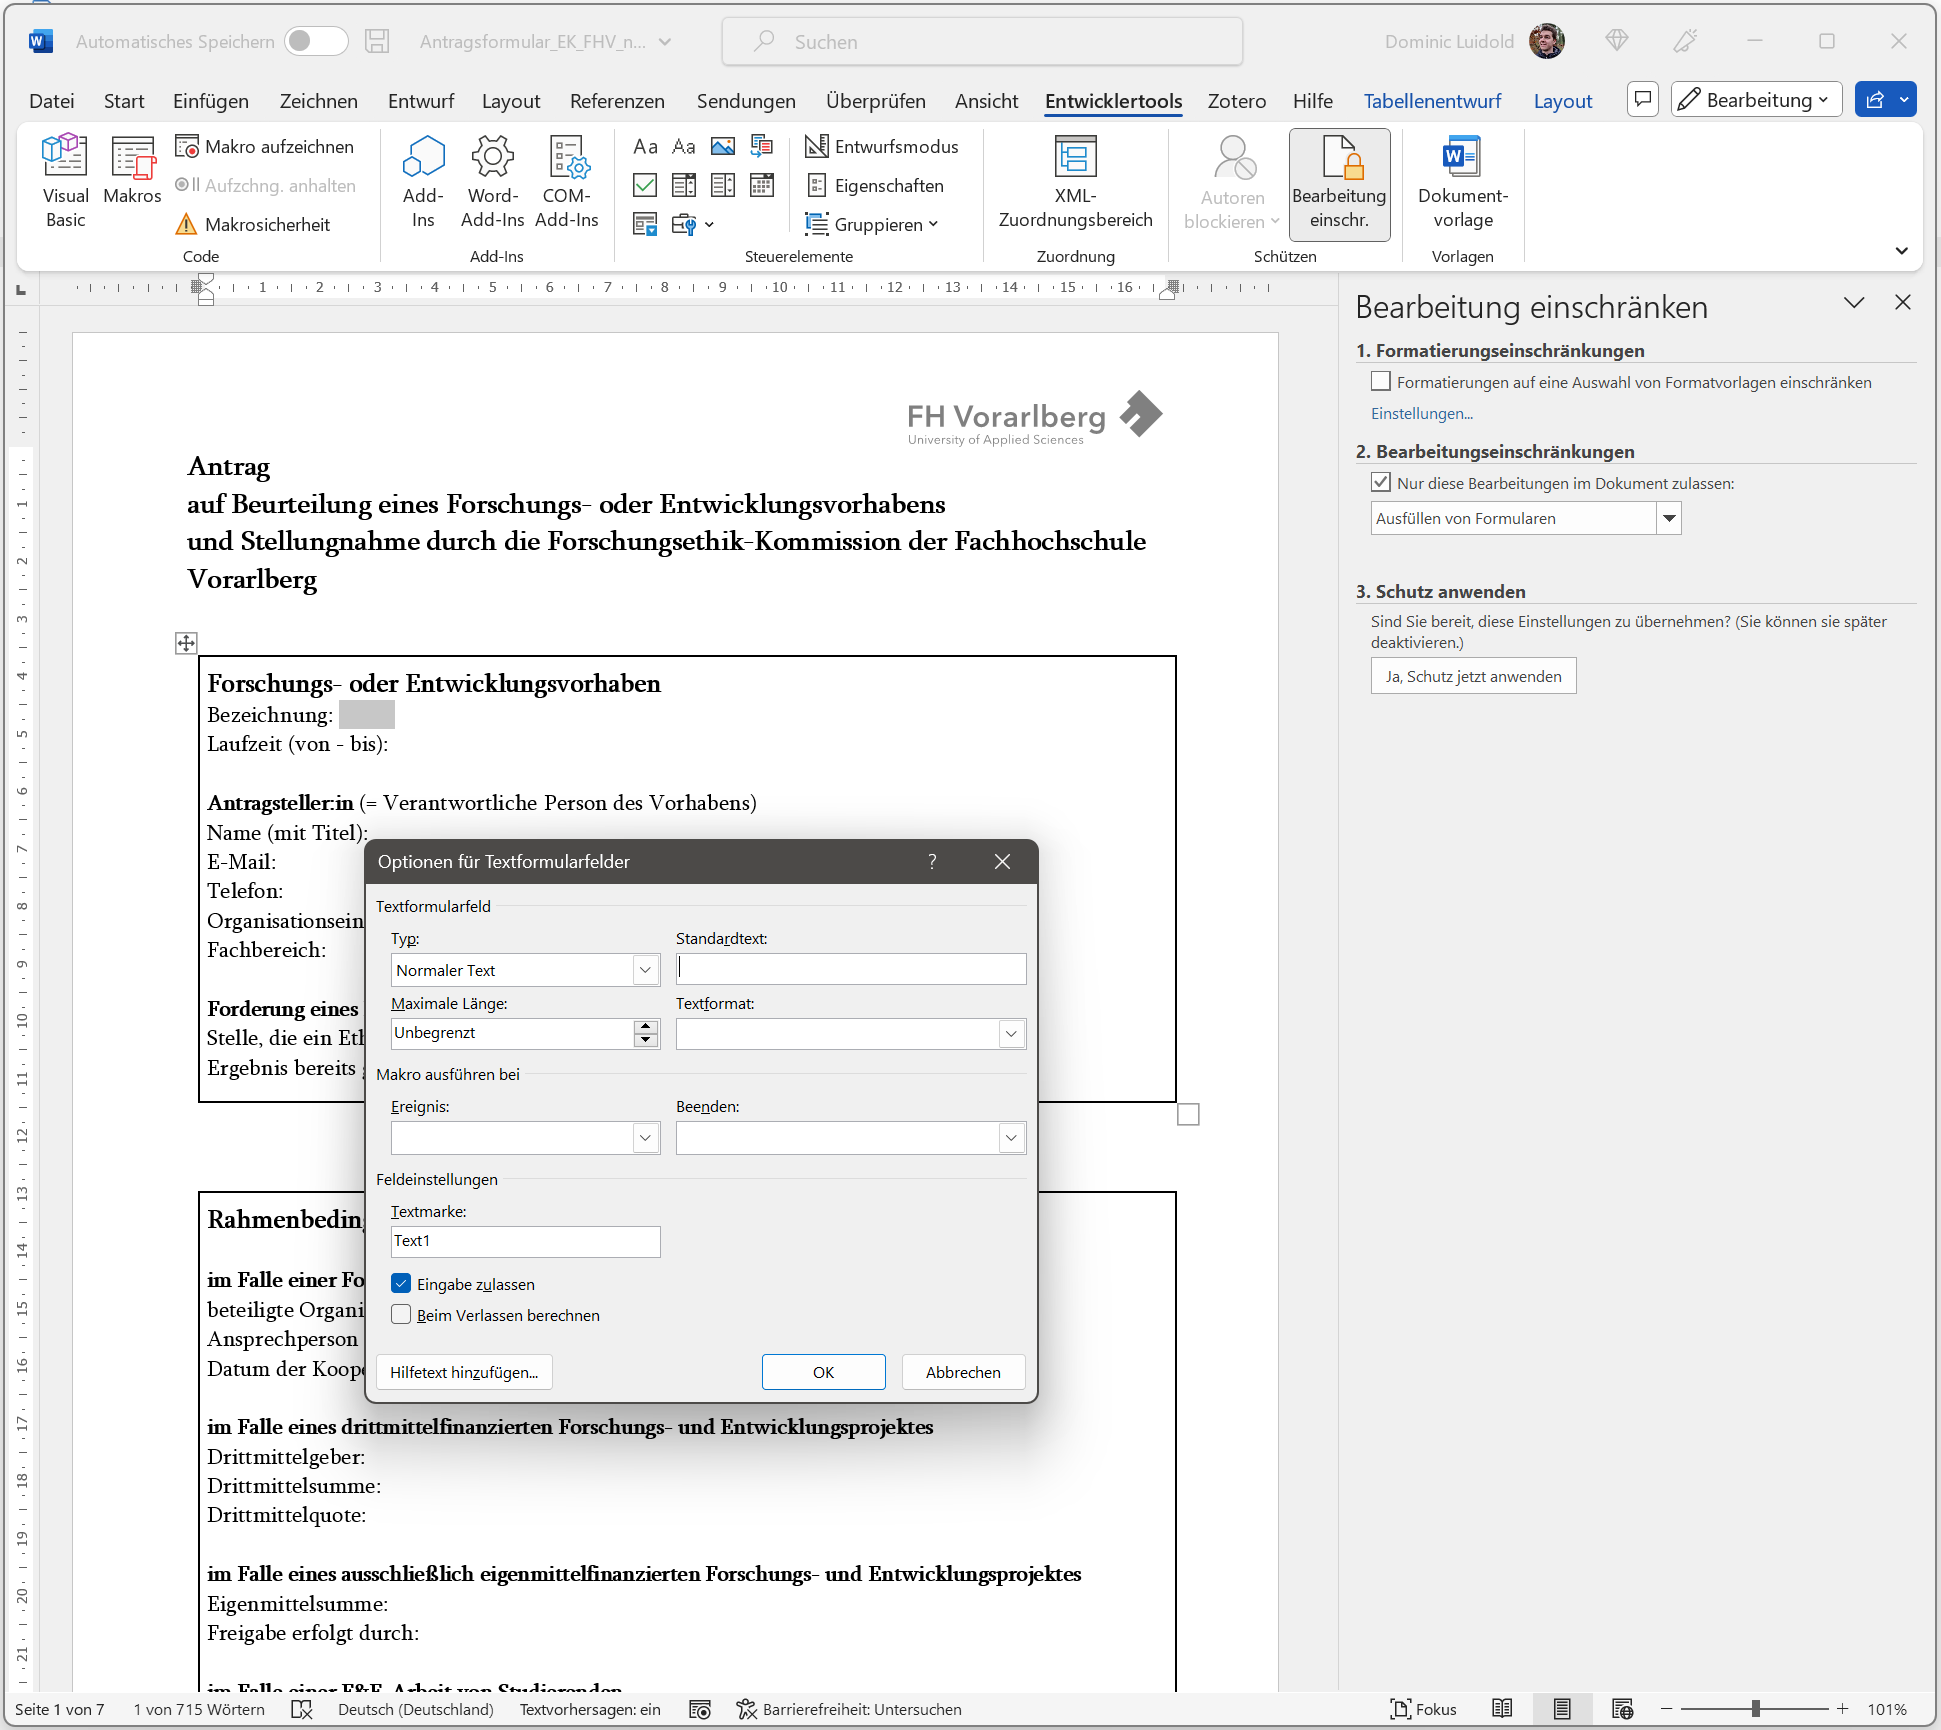
\includegraphics[width=\linewidth]{thesis/images/Luidold_Word-Vorlage-FHV-Textformularfeld.png}
    \caption{Übersicht der Optionen für Steuerelemente des Typs \texttt{Textfeld (Formularsteuerelement)} sowie die der Bearbeitungseinschränkung in Microsoft Word}
    \label{fig:optionen-textformularfeld-bearbeitungsmöglichkeiten}
\end{figure}

\subsection{Datenübermittlung}
\label{sub-sec:datenübermittlung}

Die Übermittlung des ausgefüllten Ethikantrages, sowie allfälliger Anlagen, die für eine vollständige Einreichung des Ethikantrages notwendig sein können, findet per E-Mail an den Vorsitz der \ac{fek} statt. \cite{fachhochschule_vorarlberg_gmbh_forschungsethik-kommission_2021} Die weitere Kommunikation innerhalb der Kommission selbst basiert ebenso auf der Nutzung von E-Mails, wobei die Kommission angibt (siehe Anhang \ref{appendix:gruppendiskussion} ab Seite \pageref{appendix:gruppendiskussion}), diesen Kommunikationskanal aus Datenschutzgründen so wenig wie möglich zu verwenden.

Unabhängig davon werden die eingegangen und bearbeiteten Anträge und die dazugehörigen Unterlagen auf einem Server der \acl{fhv} abgelegt und gespeichert, auf den nur Mitglieder der \ac{fek} Zugriff haben. Antragsstellende bekommen dabei eine eindeutige Nummer zugewiesen\footnote{Wie in Anhang \ref{appendix:rückmeldung-fek} ab Seite \pageref{appendix:rückmeldung-fek} ersichtlich, entspricht \texttt{23-0005-VO} der eindeutigen Nummer, die dieser Masterarbeit beziehungsweise dem dazugehörigen Ethikantrag zugewiesen wurde.}, unter der alle relevanten Dokumente geordnet auffindbar sind.

\section{Inhaltlicher Aufbau}
\label{sec:inhaltlicher-aufbau}

\subsection{Word"=Antragsvorlage}
\label{sub-sec:inhaltlicher-aufbau-word-antragsvorlage}

Wie in Abschnitt \ref{sub-sec:technischer-aufbau-word-antragsvorlage} ab Seite \pageref{sub-sec:technischer-aufbau-word-antragsvorlage} erwähnt, ist die Word"=Antragsvorlage inhaltlich in verschiedene Bereiche aufgeteilt, die unterschiedliche Fragestellungen und Themenschwerpunkte behandeln und Informationen dazu abfragen. Der Ethikantrag kann dabei in sechs inhaltliche Blöcke unterteilt werden, die in sich wiederum verschiedene Fragestellungen beinhalten:
\begin{itemize}
    \item Allgemeine Angaben zum \enquote{Forschungs- oder Entwicklungsvorhaben},
    \item Angaben zu den \enquote{Rahmenbedingungen},
    \item Erläuterungen der \enquote{Zielsetzung des Forschungs- oder Entwicklungsvorhabens},
    \item Konkrete Angaben zur \enquote{wissenschaftlichen Studie an oder mit Menschen}, sofern zutreffend,
    \item Konkrete Angaben zur \enquote{Entwicklung eines Produkts (oder Prototypen)}, sofern zutreffend sowie
    \item Angaben zum \enquote{Datenschutz in Studien oder der Produktanwendung}
\end{itemize}

Wie der Aufzählung zu entnehmen ist, ist der Ethikantrag inhaltlich breit gefächert und vereint verschiedene Fragestellungen und Themenschwerpunkte in einem Formular. Im Antrag sind sowohl Fragen zu \enquote{wissenschaftlichen Studien an oder mit Menschen} als auch zur \enquote{Entwicklung von Produkten (oder Prototypen)} enthalten, unabhängig davon, ob diese in den durchgeführten Arbeiten jeweils gemeinsam vorkommen. Diese breite Fächerung ist auf die verschiedenen Forschungszentren und die damit verbundenen Forschungsvorhaben beziehungsweise Produktentwicklungen zurückzuführen, die an der \acl{fhv} durchgeführt werden.

\medskip

Neben den Rahmenbedingungen und der Zielsetzung, welche allgemeine und unabhängige Fragestellungen darstellen, bilden die verbleibenden drei Themenblöcke den Hauptteil des Ethikantrages. Diese sind von entscheidender Bedeutung für die \ac{fek}, um wichtige Informationen für die abschließende ethische Bewertung zu erhalten. Wie bereits angesprochen, hängt der Detaillierungsgrad sowie die Anzahl an zu beantwortenden Fragen davon ab, was für eine Forschungsarbeit umgesetzt wird. Im Falle einer Studie an oder mit Menschen müssen Antragsstellende beispielsweise Informationen zum Forschungsdesign, den untersuchten Personen oder auch möglichen Risiken bereitstellen, während im Falle einer Produktentwicklung oder einer Prototypentwicklung weiterführende Angaben zum Zweck, Vorteilen oder Haftungsfragen gemacht werden müssen. Unabhängig vom entwickelten Produkt oder der durchgeführten Studie sind Fragen zum Datenschutz zu beantworten, die von der \ac{fek} genutzt werden, um daraus etwaige ethische Implikationen abzuleiten.

Der im Rahmen dieser Masterarbeit gestellte Ethikantrag (siehe Anhang \ref{appendix:eingereichter-ethikantrag} ab Seite \pageref{appendix:eingereichter-ethikantrag}) stellt in allen sechs Bereichen Informationen zur Verfügung, da sowohl eine Studie mit Menschen durchgeführt wird (in Form der Einzelinterviews beziehungsweise der Gruppendiskussion) als auch die Umsetzung eines Produkts (in Form eines Prototyps) Teil dieser Arbeit ist.

\subsection{Zusätzliche Anlagen}
\label{sub-sec:inhaltlicher-aufbau-zusätzliche-anlagen}

Um als vollständiger Ethikantrag eingereicht werden zu können, umfasst der Antrag -- neben der ausgefüllten Word"=Antragsvorlage -- zusätzlich folgende Unterlagen, die bei entsprechendem Studiendesign beziehungsweise Forschungsprojekt von der \ac{fek} gefordert sind \cite{fachhochschule_vorarlberg_gmbh_forschungsethik-kommission_2021} und, wie in Abschnitt \ref{sub-sec:datenübermittlung} ab Seite \pageref{sub-sec:datenübermittlung} angesprochen, ebenso übermittelt werden müssen:
\begin{itemize}
    \item Informierte Einwilligungserklärung (siehe als Beispiel dazu Anhang \ref{appendix:informed-consent-einzelinterview} ab Seite \pageref{appendix:informed-consent-einzelinterview}),
    \item angewandte Befragungsinstrumente (siehe als Beispiel dazu \colorbox{yellow}{TODO}) sowie
    \item von anderen Ethikkommissionen erhaltene Voten, die der Verfahrensordnung der \ac{fek} entsprechen
\end{itemize}

\section{Stärken, Schwächen \& Probleme}
\label{sec:stärken-schwächen-probleme}

Wie in Kapitel \ref{chap:einleitung} ab Seite \pageref{chap:einleitung} bereits initial angesprochen wurde, stößt die aktuell eingesetzte Word"=Antragsvorlage stellenweise sowohl auf technische als auch auf inhaltliche Limitierungen. Diese Limitierungen kommen nicht nur während des Erstellens und Ausfüllens des Ethikantrages auf, sondern sind auch im Vorfeld zur Entscheidung für einen Ethikantrag und im weiteren Verlauf des Prozesses bemerkbar.

Der nachfolgende Abschnitt beschäftigt sich daher auf Basis der Analyse der Interviews sowie der Gruppendiskussion mit den Schwächen und Problemen des aktuellen Systems, sowohl aus Sicht der \ac{fek} als auch aus Sicht von Antragsstellenden (eine detaillierte Analyse einschließlich einer entsprechenden Kategorisierung der Interviews sowie der Gruppendiskussion findet in Kapitel \ref{chap:anforderung-neues-system} ab Seite \pageref{chap:anforderung-neues-system} statt). Etwaige Stärken, die das aktuelle System vorweist, werden dabei nicht außer Acht gelassen und ebenso genauer betrachtet und hervorgehoben. 

\subsection{Sicht der Antragsteller:innen}
\label{sub-sec:probleme-sicht-Antragsteller}

In den durchgeführten Interviews mit Forschenden der \ac{fhv} (siehe Anhang \ref{appendix:interview-1} ab Seite \pageref{appendix:interview-1} sowie Anhang \ref{appendix:interview-2} ab Seite \pageref{appendix:interview-2}), die bereits einen Ethikantrag gestellt und eingereicht haben, sind unterschiedliche Themen und Anliegen zur Sprache gekommen, die den allgemeinen Prozess und auch konkret die Word"=Antragsvorlage betreffen.

Grundlegend wird die Arbeit der \ac{fek} von beiden Interviewpartner:innen geschätzt und als wichtiges Instrument empfunden, um Feedback für Forschungsprojekte und -vorhaben zu erhalten. Auch der zugrundeliegende Prozess wurde in beiden Interviews als überwiegend klar und verständlich eingeschätzt. Im Verlauf der Interviews und bei genauerem Nachfragen wurden dennoch einige Punkte angeführt, welche bei den Forschenden \enquote{negativ} in Erinnerung geblieben sind beziehungsweise laut ihnen auch Verbesserungspotenzial aufweisen:
\begin{itemize}
    \item die Kommunikation und Einreichung des Ethikantrages mittels E-Mail zwischen Antragsteller:in und \ac{fek},
    \item eine fehlende Hilfestellung in der Entscheidung zum Ethikantrag und weitere Unterstützung,
    \item Schwierigkeiten beim Ausfüllen des Ethikantrages aufgrund technischer Hürden,
    \item die inhaltliche Wiederholungen in den Fragestellungen der Themenschwerpunkte sowie
    \item Detailfragen zum Prozessablauf bei Auflagen der \ac{fek}
\end{itemize}

\subsubsection*{Kommunikation mittels E-Mail}
\label{sub-sub-sec:kommunikation-email}

In beiden Interviews kommt zur Sprache, dass das Einreichen des Ethikantrages und der entsprechenden Anlagen sowie der Erhalt der abschließenden Stellungnahme und des Votums per E-Mail nicht optimal ist. Einerseits müssen die erstellten Unterlagen -- stellenweise mehrfach -- hin und her gesendet werden, wodurch schnell der Überblick über die verschiedenen Dateiversionen verloren geht. Andererseits führt die allgemein bereits große Anzahl an E-Mails laut den Forschenden dazu, dass wichtige Nachrichten und die ebenfalls per E-Mail stattfindende Kommunikation mit der \ac{fek} übersehen werden könnte.

\subsubsection*{Hilfestellung zur Entscheidung und weitere Unterstützung}
\label{sub-sub-sec:hilfestellung-unterstützung}

Einer der ehemaligen Antragsstellenden spricht im Interview an, dass es nicht in allen Fällen eindeutig beziehungsweise von Beginn an klar ist, ob ein Ethikantrag und das Einholen eines ethischen Votums für das Forschungsprojekt oder das Forschungsvorhaben überhaupt notwendig ist und welche Kriterien dafür ausschlaggebend sind. Ebenso wird thematisiert, dass die Word"=Antragsvorlage nur begrenzt Hilfestellungen bietet und mehr Führung durch den konkreten Antrag sinnvoll sein könnte, aktuell jedoch ausbleibt.

\subsubsection*{Technische Hürden}
\label{sub-sub-sec:technische-hürden}

In einem der Interviews wird auf technische Schwierigkeiten hingewiesen, die beim Ausfüllen der Word"=Antragsvorlage auftreten können. Insbesondere gibt es Probleme bei der Eingabe von Text in den Formularfeldern, die in Abschnitt \ref{sub-sec:technischer-aufbau-word-antragsvorlage} ab Seite \pageref{sub-sec:technischer-aufbau-word-antragsvorlage} erwähnt werden. Konkret wird im Interview berichtet, dass die Nutzerfreundlichkeit vor allem unter dem macOS-Betriebssystem von Apple fehlerhaft oder eingeschränkt ist, da sich beispielsweise die Cursor-Position ungewollt verschieben kann, wodurch die Texteingabe erschwert wird.

\subsubsection*{Inhaltliche Wiederholungen}
\label{sub-sub-sec:inhaltliche-wiederholungen}

Neben den technischen Hürden der Word"=Antragsvorlage werden die von der \ac{fek} gestellten Fragen in den in Abschnitt \ref{sub-sec:inhaltlicher-aufbau-word-antragsvorlage} ab Seite \ref{sub-sec:inhaltlicher-aufbau-word-antragsvorlage} dargelegten sechs Themenbereichen kritisiert, da sich -- bei einem entsprechendem Projekt -- inhaltliche Wiederholungen und Überschneidungen ergeben, die womöglich vermieden werden könnten.

\subsubsection*{Detailfragen zum Prozessablauf}
\label{sub-sub-sec:detailfragen-prozessablauf}

Im Verlauf beider Interviews wird der Erhalt der abschließenden Stellungnahme mit entsprechenden Auflagen thematisiert. Eine:r der Forschenden äußert dabei die Frage, ob es erforderlich ist, nach der Einarbeitung von Auflagen oder Verbesserungsvorschlägen den Antrag erneut einzureichen oder ob dies nicht mehr notwendig ist beziehungsweise ob ein weiteres \enquote{Hin und Her} zwischen Antragsteller:in und \ac{fek} ausgelassen werden kann. Die Aussage der zweiten Interviewpartner:in legt nahe, dass in Bezug auf diesen Schritt möglicherweise Unklarheiten im Prozess bestehen, da der Schritt dort als fixer Bestandteil des Prozesses wahrgenommen wird.

\subsection{Sicht der \acl{fek}}
\label{sub-sec:probleme-sicht-fek}

Aus Sicht der \acl{fek} gibt es im Rahmen der Gruppendiskussion (siehe Anhang \ref{appendix:gruppendiskussion} ab Seite \pageref{appendix:gruppendiskussion}) grundsätzlich nur wenige konkrete Bedenken oder Probleme am aktuell festgelegten Prozess und der Word"=Antragsvorlage, die Antragsteller:innen zur Verfügung gestellt wird. Primär deshalb, da der Prozess und die angebotene Antragsvorlage von den aktuellen Kommissionsmitgliedern maßgeblich mitgestaltet und erstellt wurde.

Nichtsdestotrotz sind im Verlauf des Gespräches mehrere Themen zur Sprache gekommen, bei denen die Kommission selbst sowohl Stärken in der Vorgehensweise als auch Potenzial für Veränderungsmöglichkeiten sieht, die sowohl für diese Masterarbeit relevant sind als auch solche, die diese unberührt lassen:
\begin{itemize}
    \item E-Mail als Kommunikationskanal,
    \item der administrative Aufwand,
    \item den inhaltlichen Aufbau mit gezielter Struktur,
    \item Möglichkeiten zur Formatierung und Funktionseinschränkungen der Word"=Antragsvorlage sowie
    \item eine generelle Umstrukturierung des Prozesses mit verpflichtender Präsentation als fixer Bestandteil
\end{itemize}

\subsubsection*{E-Mail als Kommunikationskanal}
\label{sub-sub-sec:email-kommunikationskanal}

Die Mitglieder der Kommission weisen in der Gruppendiskussion darauf hin, dass die Kommunikation und der Austausch von Antragsunterlagen per E-Mail zwar stattfindet, aber aus Datenschutzgründen weitestgehend vermieden wird. Stattdessen wird in der internen Kommunikation auf einen sicheren Server der \acl{fhv} zurückgegriffen, wie in Abschnitt \ref{sub-sec:datenübermittlung} ab Seite \ref{sub-sec:datenübermittlung} bereits angesprochen wurde. Da antragsstellende Personen einen Antrag jedoch initial per E-Mail übermitteln müssen, kann die Kommission diesen Kommunikationskanal nicht, wie im Gespräch gewünscht, vollständig vermeiden.

\subsubsection*{Administrativer Aufwand}
\label{sub-sub-sec:administrativer-aufwand}

In der Diskussion thematisiert die \ac{fek} auch den hohen administrativen Aufwand, der beim Vorsitz der Kommission liegt. Sowohl die manuelle Kommunikation in Form von Eingangs- und Bearbeitungsbestätigungen als auch der formale Vollständigkeitscheck und die Überprüfung der Antragsberechtigung müssen laut Kommission von Hand durchgeführt werden. Das aktuelle System und der Prozess lassen in diesen Bereichen keine vereinfachte Handhabung zu, was während des Gesprächs bemängelt wird.

\subsubsection*{Inhaltlicher Aufbau}
\label{sub-sub-sec:inhaltlicher-aufbau}

In der Gruppendiskussion betrachten die Kommissionsmitglieder den inhaltlichen Aufbau des Ethikantrags und der Antragsvorlage sowohl als Stärke als auch als mögliches Verbesserungspotenzial bei einer entsprechenden Überarbeitung des Sytems. Die inhaltlichen Wiederholungen, die von den Forschenden in Abschnitt \ref{sub-sub-sec:inhaltliche-wiederholungen} ab Seite \pageref{sub-sub-sec:inhaltliche-wiederholungen} stellenweise bemängelt werden, sieht die Kommission nicht nur als Problem, sondern in vielen Fällen auch als Chance für einen \enquote{Reliabilitätscheck}. Die einzelnen Mitglieder können durch die Ausführlichkeit und den hohen Detaillierungsgrad viele Informationen entnehmen und Widersprüche im Forschungsdesign und den Angaben erkennen und thematisieren.

\subsubsection*{Technische Möglichkeiten und Funktionseinschränkungen }
\label{sub-sub-sec:möglichkeiten-funktionseinschränkungen}

Im Verlauf des Gespräch mit der \acl{fek} kommen sowohl gezielte als auch ungewollte (technische) Limitierungen der Word"=Antragsvorlage zur Sprache. Die fehlenden Formatierungsmöglichkeiten innerhalb der eingesetzten Formularfelder, wie in Abschnitt \ref{sub-sec:technischer-aufbau-word-antragsvorlage} auf Seite \pageref{sub-sec:technischer-aufbau-word-antragsvorlage} erwähnt, ist von der \ac{fek} beispielsweise beabsichtigt und bekannt. Antragstellende sollen dadurch dazu ermutigt werden, sich auf gut lesbaren Inhalt zu konzentrieren, der ohne Formatierungshilfen verständlich ist. Nicht beabsichtigte Einschränkungen, über die die Kommission über Feedback von Antragsstellenden informiert wurde, umfassen laut den Interviewpartner:innen wiederum die fehlende Möglichkeit, Literaturverwaltungsprogramme wie Zotero\footnote{Zotero (\url{https://www.zotero.org/})} nutzen zu können sowie Einschränkungen beim Versuch, digitale Unterschriften direkt in der Antragsvorlage zu verwenden, um einen gültigen Antrag zu gewährleisten.

\subsubsection*{Umstrukturierung des Prozesses}
\label{sub-sub-sec:umstrukturierung-prozess}

Ein Mitglied der \ac{fek} äußert während des Interviews den Vorschlag, den Prozess grundlegend zu überdenken, um sowohl den administrativen Aufwand als auch die Belastung der Antragsteller:innen zu reduzieren und inhaltliche Wiederholungen in den Fragestellungen des Ethikantrages zu vermeiden. Die Kommission sieht die Möglichkeit, anstelle eines sehr detaillierten Antragsformulars einen kürzeren Antrag in Kombination mit einer verpflichtenden Präsentation des Forschungsvorhabens zu verwenden, ähnlich wie es andere Ethikkommissionen handhaben. Im Verlauf des Gesprächs stimmen einige der Mitglieder zu und sehen darin eine alternative Möglichkeit, auf bestimmte Aspekte des Antrages in der Präsentation genauer einzugehen um auf einem gleichen Qualitätsniveau bleiben zu können.

\chapter{Analyse anderer Prozesse}
\label{chap:analyse-anderer-prozesse}

Um neben der Analyse des bestehenden Systems beziehungsweise Prozesses rund um die Word-Antragsvorlage Vergleichswerte sammeln zu können, werden weitere Prozesse und Systeme sowohl mit spezifischem Fokus auf Ethikanträgen als auch Systeme ohne direkten Bezug genauer betrachtet und Unterschiede sowie Gemeinsamkeiten herausgearbeitet.

Durch die breiter gefasste Erhebung zum Stand der Technik können so zusätzliche Herangehensweisen, die in der Analyse in Kapitel \ref{chap:analyse-bestehendes-system-prozess} ab Seite \pageref{chap:analyse-bestehendes-system-prozess} nicht aufgegriffen werden konnten, abgedeckt werden. Ebenso kann dadurch eruiert werden, ob ein bestehendes System die Möglichkeit bietet, soweit an die in Kapitel \ref{chap:anforderung-neues-system} ab Seite \pageref{chap:anforderung-neues-system} gestellten Anforderungen der \acl{fek} sowie der Antragsteller:innen angepasst werden zu können, als das eine gänzliche Neuentwicklung nicht mehr notwendig ist.

\section{Systeme mit Fokus auf Ethikanträgen}
\label{sec:systeme-mit-fokkus-ethikantrage}

\subsection{Vorlage des Forums Österreichischer Ethikkommissionen}
\label{sub-sec:vorlage-föe}

Das \ac{föe}\footnote{Forum Österreichischer Ethikkommissionen (\url{https://me001ned.edis.at/ethikkommission/Forum/})} ist ein freiwilliger Zusammenschluss von Ethikkommissionen in Österreich mit medizinischem Fokus und mit dem Hintergrund, einheitliche Arbeitsweisen und Formulare (für beispielsweise Meldungen, Anträge etc.) für österreichiche Ethikkommissionen zu schaffen. \cite{ethikkommission_der_medizinischen_universitat_graz_forum_2019}

\subsubsection*{Allgemeiner Aufbau}
\label{sub-sub-sec:föe-allgemeiner-aufbau}

Ähnlich zur Herangehensweise der \acl{fek} der \acl{fhv} basieren die vom \ac{föe} bereitgestellten Unterlagen auf Dokumentenvorlagen im \texttt{.dot} beziehungsweise \texttt{.rtf} Dateiformat, wobei die Nutzung von Microsoft Word vom Forum ausdrücklich empfohlen wird. Neben dem zum Download angebotenen Antrag\footnote{Antragsformular in der Version 6.4 vom 12.06.2012 (\url{https://me001ned.edis.at/ethikkommission/Forum/Download/Files/Antr.dot})} werden zusätzlich ein ausgefülltes Muster sowie Erläuterungen zum Antrag im \texttt{.pdf} Dateiformat beigelegt, welche erklären, wie die Vorlage geöffnet, ausgefüllt und gespeichert werden kann.\footnote{Die bereitgestellten Erläuterungen stammen aus dem Jahr 2004, weshalb diese aller Wahrscheinlichkeit nach so detailliert ausfallen (beispielsweise die Bezugnahme auf die Menüführung des damaligen \enquote{WinWord}).} \cite{ethikkommission_der_medizinischen_universitat_graz_download_2012}

\medskip

Die in Abbildung \ref{fig:dokumentenvorlage-föe} auf Seite \pageref{fig:dokumentenvorlage-föe} dargestellte Antragsvorlage führt die Antragsteller:innen durch zwei verschiedene Teile (\enquote{Teil A} und \enquote{Teil B}), in denen unterschiedliche Angaben entweder in Freitext-Formularfeldern oder in entsprechend anzukreuzenden Auswahl-Feldern\footnote{Aufgrund der verwendeten Einschränkung der Bearbeitungsmöglichkeiten (siehe vergleichsweise dazu Abschnitt \ref{sub-sec:technischer-aufbau-word-antragsvorlage} ab Seite \pageref{sub-sec:technischer-aufbau-word-antragsvorlage}) mit zusätzlichem Passwordschutz kann nicht nachvollzogen werden, welchen Typ diese Felder haben.} gemacht und Fragen beantwortet werden können.

\begin{figure}[ht]
    \centering
    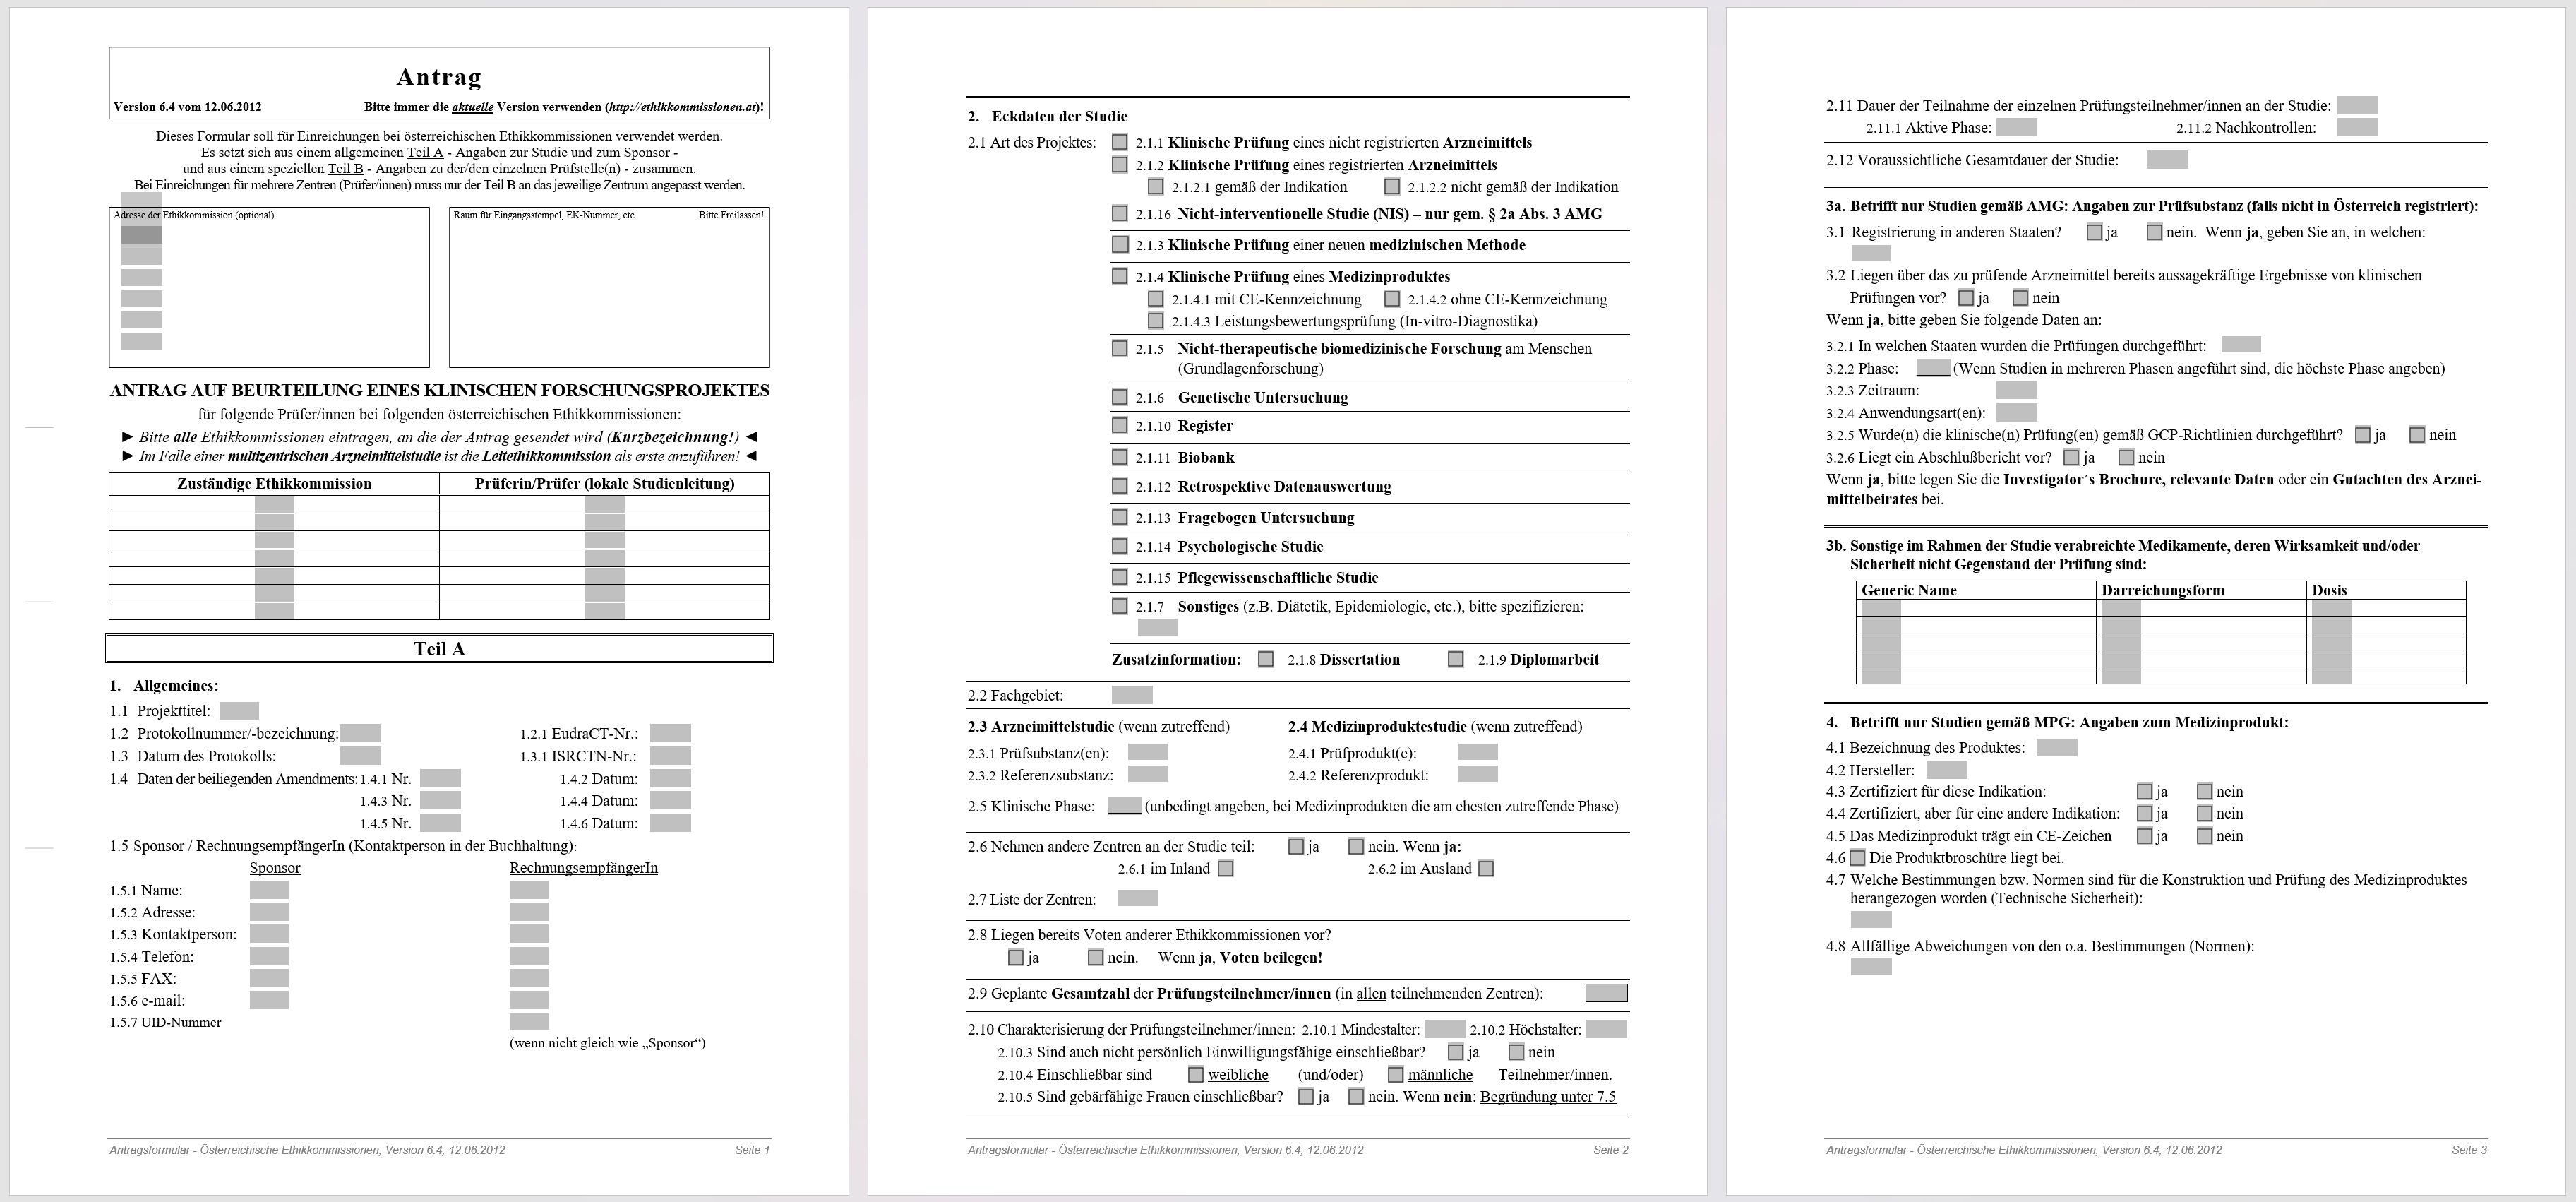
\includegraphics[scale=0.21]{thesis/images/Luidold_Word-Vorlage-Forum-Oesterreichischer-Ethikkommissionen.png}
    \caption[Word"=Antragsvorlage des Forums Österreichischer Ethikkommissionen]{Word"=Antragsvorlage des Forums Österreichischer Ethikkommissionen \cite{ethikkommission_der_medizinischen_universitat_graz_download_2012}}
    \label{fig:dokumentenvorlage-föe}
\end{figure}

\subsubsection*{Inhaltlicher Aufbau}
\label{sub-sub-sec:föe-inhaltlicher-aufbau}

Alle zu befüllenden Felder sind mit einer eindeutigen Nummer gekennzeichnet und sind dabei auf insgesamt 14 Themenblöcke aufgeteilt, die sich, wie angesprochen, in \enquote{Teil A} und \enquote{Teil B} aufgliedern. Die zu beantwortenden Fragen des ersten Teils beinhalten vom Projekttitel über detaillierte Angaben von geplanten Therapie- und Diagnostikverfahren bis hin zu Angaben zu Biometrie und Datenschutz Informationen mit Fokus auf den medizinischen Aspekten der durchgeführten Studie. Der zweite Teil umfasst hauptsächlich Angaben zu den durchführenden Prüfer:innen der Studie sowie Fragen zu den verantwortlichen Mitarbeitenden.

\subsubsection*{Ähnlichkeiten \& Auffälligkeiten}
\label{sub-sub-sec:ähnlichkeiten-auffälligkeiten-föe}

Bei der Durchsicht des Antrages fallen folgende Punkte im Vergleich zur Herangehensweise der \ac{fek} konkret auf:
\begin{itemize}
    \item Die Vorlage enthält sowohl für die finale Beurteilung benötigte Informationen (die durch die Antragsteller:innen bereitgestellt werden) als auch Ausfüllhilfen und Hilfestellungen, die zwischen den einzelnen Punkten und Fragen eingebettet sind.
    \item Gewisse Tabellen (wie beispielsweise die Tabellen bei Punkt \enquote{6. Angaben zur durchzuführenden Therapie und Diagnostik} auf Seite 5 des Antrages) lassen nur eine gewisse Anzahl an Einträgen zu, ohne den Antragsstellenden die Möglichkeit zu geben, weitere Punkte hinzufügen zu können.
    \item Es stehen ebenso keinerlei Formatierungsmöglichkeiten zur Verfügung, um ausgefüllte Informationen beispielsweise mit kursiver oder farbig hinterlegter Schrift zu strukturieren. Alle getätigten Informationen sind automatisch in fetter Schrift angegeben, um sie von der Vorlage unterscheiden zu können.
\end{itemize}

Da das \ac{föe} keine eigenständige Ethikkommission bildet, hängt der Prozess des Einreichens des erstellten und ausgefüllten Ethikantrages von der jeweiligen Ethikkommmission ab. Das Forum weist jedoch darauf hin, dass es trotz der einheitlichen Formulare zusätzliche Anforderungen geben kann oder das Formular gar nicht mehr in Form der zum Download angebotenen Antragsvorlage angenommen wird (siehe Abschnitt \ref{sub-sec:ecs} ab Seite \pageref{sub-sec:ecs} für weiterführende Informationen dazu). \cite{ethikkommission_der_medizinischen_universitat_graz_download_2012}

\subsubsection*{Schlussfolgerungen}
\label{sub-sub-sec:schlussfolgerungen-föe}

Aufgrund der thematischen Ausrichtung des \acl{föe} auf medizinische Ethikkommissionen ergeben sich aus der vorliegenden Antragsvorlage nur begrenzt übertragbare Anforderungen für den in der vorliegenden Masterarbeit zu entwickelnden Lösungsansatz. Dies ist insbesondere darauf zurückzuführen, dass die Antragsvorlage beinahe idente Ansätze zu denen der Vorlage der \acl{fek} der \acl{fhv} verwendet.

\subsection{Vorlage der FH Gesundheitsberufe OÖ}
\label{sub-cec:vorlage-fh-oö}

Das \ac{ieb}\footnote{Institutionelles Ethikboard der FH Gesundheitsberufe OÖ (\url{https://www.fh-gesundheitsberufe.at/f-e/institutionelles-ethikboard/})} fokussiert sich auf die Überprüfung ethischer Aspekte bei eingereichten Forschungsprojekten an oder mit Menschen und darauf, ob eine zusätzliche Einreichung bei einer spezialisierten Ethikkommission notwendig ist. \cite{fh_gesundheitsberufe_oo_gmbh_institutionelles_2023}

\medskip

Der Prozess der Einreichung eines Ethikantrages wird vom \ac{ieb} in einen zweistufigen Prozess unterteilt, welcher detailliert in Abbildung \ref{fig:prozess-ethikantrag-ieb} auf Seite \pageref{fig:prozess-ethikantrag-ieb} dargestellt wird. Nach initialer Überprüfung der Vollständigkeit wird der eingereichte Ethikantrag von zwei dem Ethikboard angehörigen Mitgliedern geprüft und entschieden, ob eine direkte Behandlung durch das \ac{ieb} möglich ist oder ob dieser bei einer spezialisierten Kommission eingereicht werden muss. Verläuft die weitere Prüfung positiv, kann dem Antrag entweder eine \enquote{Unbedenklichkeitsbescheinigung} ausgestellt werden oder es findet eine detaillierte Prüfung in einer Vollversammlung des \ac{ieb} statt, die bei Erfülllung etwaiger Auflagen in einem positiven Votum endet. \cite{fh_gesundheitsberufe_oo_gmbh_einreichung_2023}

\begin{figure}[ht]
    \centering
    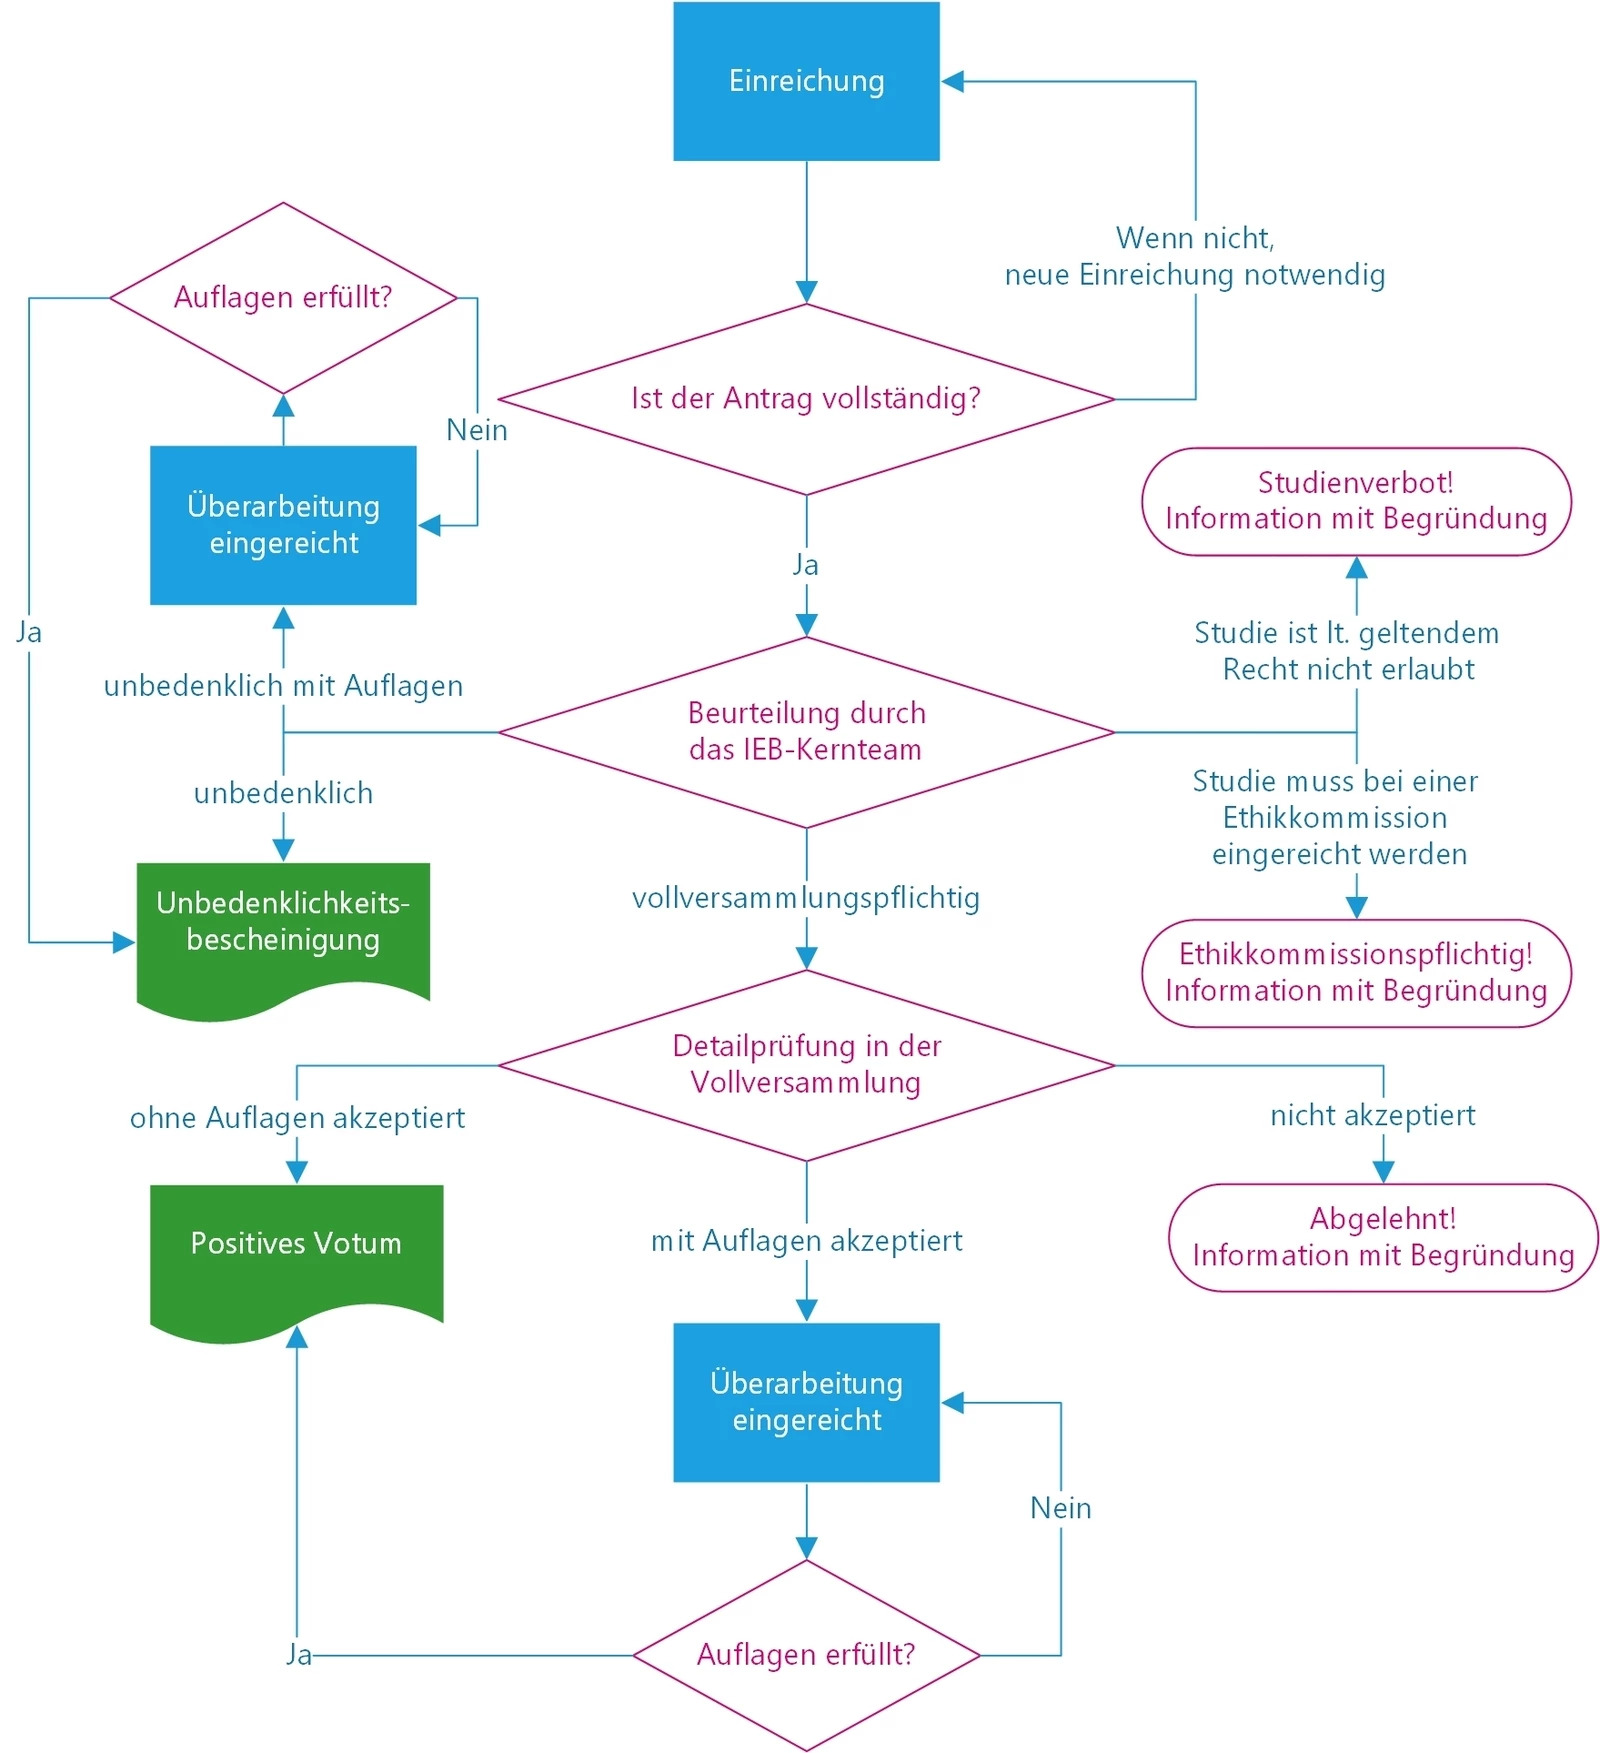
\includegraphics[scale=0.15]{thesis/images/FHGOOE_Prozess-Ethikantrag.jpg}
    \caption[Prozessdiagramm zur Einreichung eines Ethikantrages beim Institutionellen Ethikboard der FH Gesundheitsberufe OÖ]{Prozessdiagramm zur Einreichung eines Ethikantrages beim Institutionellen Ethikboard der FH Gesundheitsberufe OÖ \cite{fh_gesundheitsberufe_oo_gmbh_einreichung_2023}}
    \label{fig:prozess-ethikantrag-ieb}
\end{figure}

\subsubsection*{Allgemeiner Aufbau}
\label{sub-sub-sec:fh-oö-allgemeiner-aufbau}

Das \ac{ieb} greift -- ebenso wie das \ac{föe} und die \ac{fek} der \ac{fhv} -- auf eine Antragsvorlage\footnote{Antragsformular Version 1 vom 21.09.2022 (\url{https://www.fh-gesundheitsberufe.at/assets/files/IEB-Antragsformular_V1.00_21.09.2022.docx})} im mit Microsoft Word kompatiblen \texttt{.docx} Dateiformat zurück. Diese Vorlage wird Antragsteller:innen zum Download angeboten und kann sowohl digital als auch in einer Printversion beim Ethikboard zur Begutachtung eingereicht werden. \cite{fh_gesundheitsberufe_oo_gmbh_einreichung_2023}

\medskip

Abbildung \ref{fig:dokumentenvorlage-ieb} auf Seite \pageref{fig:dokumentenvorlage-ieb} zeigt einen Ausschnitt des Dokumentes, welches sowohl mittels Freitext-Feldern des Typs \texttt{Textfeld (Formularsteuerelement)} und Kontrollkästchen des Typs \texttt{Kontrollkästchen (Formularsteuerelement)} als auch ohne jegliche Formular- beziehungsweise Steuerelemente arbeitet und Informationen abfragt. Auffallend ist, dass das gesamte Dokument von antragsstellenden Personen nach belieben bearbeitet werden kann, da eine Einschränkung der Bearbeitungsmöglichkeiten (siehe vergleichsweise dazu Abschnitt \ref{sub-sec:technischer-aufbau-word-antragsvorlage} ab Seite \pageref{sub-sec:technischer-aufbau-word-antragsvorlage}) ausbleibt. Theoretisch können somit beispielsweise Hilfestellungen, Fragen und anderweitige Inhalte des Antrages bearbeitet oder auch gänzlich entfernt werden. Ebenso stehen alle gängigen Formatierungsmöglichkeiten, wie beispielsweise unterstrichener, kursiver oder farbig hinterlegter Text, zur Verfügung.

\begin{figure}[ht]
    \centering
    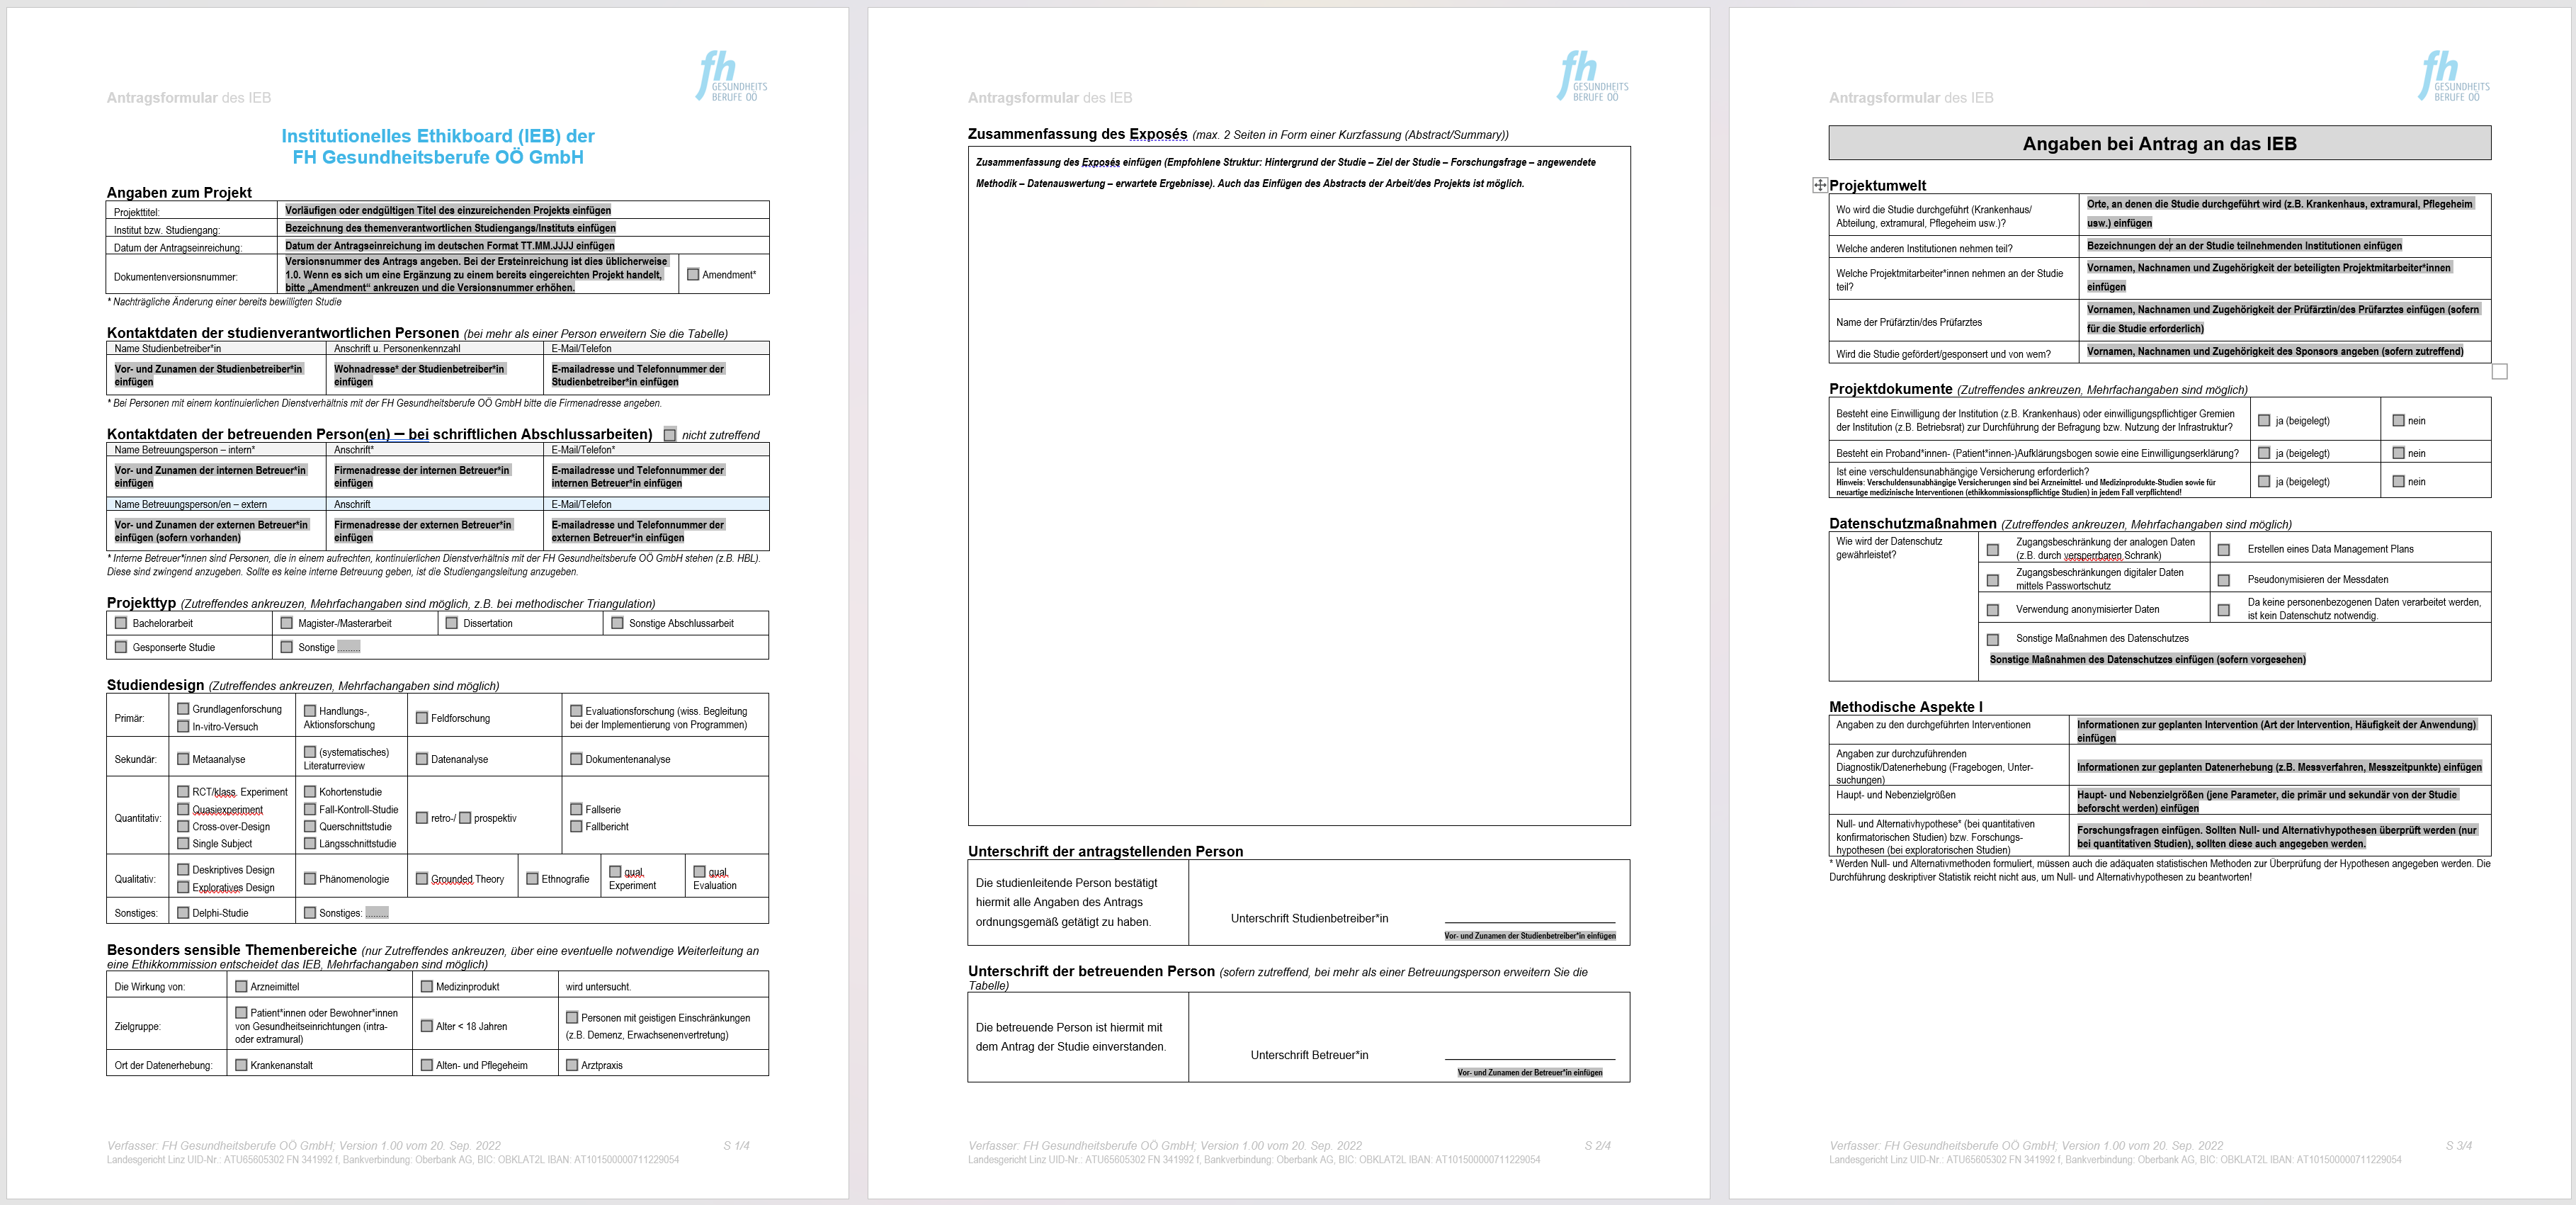
\includegraphics[scale=0.21]{thesis/images/Luidold_Word-Vorlage-IEB-FH-Gesundheitsberufe-OOE.png}
    \caption[Word"=Antragsvorlage des Institutionellen Ethikboards der Fachhochschule Gesundheitsberufe OÖ]{Word"=Antragsvorlage des Institutionellen Ethikboards der Fachhochschule Gesundheitsberufe OÖ \cite{fh_gesundheitsberufe_oo_gmbh_dokumente_2023}}
    \label{fig:dokumentenvorlage-ieb}
\end{figure}

\subsubsection*{Inhaltlicher Aufbau}
\label{sub-sub-sec:fh-oö-inhaltlicher-aufbau}

Das vom \ac{ieb} zum Download angebotene Antragsformular weicht, trotz des Fokus auf medizinische Studien der Fachhochschule und des Boards, sowohl vom Aufbau als auch vom abgefragten Inhalt von der Antragsvorlage des \ac{föe} ab. Das \ac{ieb} erläutert, dass die eigens umgesetzte Word"=Antragsvorlage gezielt nicht an jene des \ac{föe} angelehnt ist, da sich das Formular des \ac{föe} als zu detailliert und zeitaufwendig in der Bearbeitung herausstellt, sowohl für Antragsteller:innen als auch für die Prüfung selbst. Als zweiter Grund wird auch beziehungsweise vor allem der Umstand genannt, dass vom \ac{ieb} alle Arbeiten geprüft und behandelt werden müssen, die nicht ausschließlich eine Literaturarbeit darstellen. \cite{rosendahl-huber_extern-erfahrungen_2023}

\medskip

Unabhängig vom abweichenden Aufbau fokussiert sich der Antrag auf Angaben zur geplanten Studie und stellt Fragen in Bezug auf die konkrete Projektumwelt anhand von teilnehmenden Institutionen und Prüfer:innen, Datenschutzmaßnahmen, Studiendesign und methodische Aspekte. Das Antragsformular bietet auf Seite 2 zudem die Möglichkeit, eine Zusammenfassung des Exposés oder des Abstracts der Forschungsarbeit einzureichen.\footnote{Dieser Schritt wird von der \ac{fek} der \ac{fhv} ebenso als Möglichkeit gesehen (siehe Anhang \ref{appendix:gruppendiskussion} ab Seite \pageref{appendix:gruppendiskussion}), um die Anzahl an Fragen im Antragsformular zur verringern und Antragsteller:innen die Möglichkeit zu geben, bereits ausgearbeitete Informationen wiederzuverwenden.}

\subsubsection*{Ähnlichkeiten \& Auffälligkeiten}
\label{sub-sub-sec:ähnlichkeiten-auffälligkeiten-fh-oö}

Laut dem \ac{ieb} sind derzeit zwei digitale Lösungen in Entwicklung, die die erst seit September 2022 veröffentlichte Word"=Antragsvorlage langfristig ablösen sollen, um den Prozess zu vereinfachen und den Arbeitsaufwand sowie aktuell auftretende Übertragungsfehler zu minimieren. Der erste der zwei geplanten Lösungsansätze basiert dabei auf einem Webformular, das eingelangte Informationen per E-Mail an das \ac{ieb} übermitteln soll, während die schlussendlich angedachte Lösung den gesamten Prozess und das Antragswesen in einem konkret dafür ausgelegten System abbilden soll. \cite{rosendahl-huber_extern-erfahrungen_2023}

\subsubsection*{Schlussfolgerungen}
\label{sub-sub-sec:schlussfolgerungen-fh-oö}

Vergleichbar zu der in Abschnitt \ref{sub-sec:vorlage-föe} ab Seite \pageref{sub-sec:vorlage-föe} durchgeführten Analyse des \ac{föe} lassen sich auf Basis des Systems des \ac{ieb} keine konkreten Schlüsse für die praktische Ausarbeitung eines neuen Systems ziehen, da zum Zeitpunkt der Ausarbeitung dieser Arbeit ebenfalls eine Word"=Antragsvorlage zum Einsatz kommt. Als möglicher Anhaltspunkt dient jedoch das in Abbildung \ref{fig:prozess-ethikantrag-ieb} auf Seite \pageref{fig:prozess-ethikantrag-ieb} dargestellte Prozessdiagramm, welches in adaptierter Form in die Neuentwicklung des Systems als Hilfestellung einfließen könnte, um Antragsteller:innen den gesamten Prozess der \ac{fek} der \ac{fhv} übersichtlich darstellen zu können. Die geplanten Lösungsansätze des \ac{ieb} zur Ablösung der bisherigen Vorlage bieten zudem einen Anhaltspunkt, wie eine ähnliche Umsetzung im Rahmen dieser Masterarbeit aussehen könnte.

\subsection{Einreichplattform der FH Campus Wien}
\label{sub-sec:einreichplattform-fh-campus-wien}

Die FH Campus Wien verfügt seit 2021 über eine eigene Ethikkommission\footnote{Ethikkommission für Forschungsaktivitäten (\url{https://www.fh-campuswien.ac.at/forschung/ethikkommission-fuer-forschungsaktivitaeten.html})}, die ihren Ursprung im 2014 an der FH Campus Wien gegründeten Ethik-Komitee hat. Die Ethikkommission unterstützt dabei Forschende bei Anliegen und Fragen im Bereich von ethischen Fragestellungen sowie zu Rechtsvorschriften und Themen, die den Datenschutz betreffen und prüft Forschungsprojekte sowie Forschungsarbeiten auf ethische Aspekte. \cite{fh_campus_wien_ethikkommission_2023}

\subsubsection*{Allgemeiner Aufbau}
\label{sub-sub-sec:fh-cw-allgemeiner-aufbau}

Die Ethikkommission der FH Campus Wien setzt auf eine online abrufbare Einreichplattform\footnote{Einreichplattform für Anträge bei der Ethikkommission der FH Campus Wien (\url{https://ethikantrag.fh-campuswien.org/})}, die von Antragsteller:innen genutzt werden kann, um Ethikanträge digital erstellen und einreichen zu können. \cite{ethikkommission_fh_campus_wien_fh_2023} Die Einreichplattform ermöglicht Antragstellenden dabei die Verwaltung und Einsichtnahme von offenen, eingereichten und abgeschlossenen Ethikanträgen. Abbildung \ref{fig:startseite-einreichplattform-fhcw} auf Seite \pageref{fig:startseite-einreichplattform-fhcw} zeigt die Start- beziehungsweise Übersichtsseite im eingeloggtem Zustand, auf der die Anträge in den drei genannten Kategorien eingesehen werden können. Neben der Möglichkeit zur Einsicht in bestehende Anträge bietet die Startseite auch die Möglichkeit, einen neuen Ethikantrag zu stellen sowie über die Menü-Leiste zum Download-Bereich zu navigieren.

\begin{figure}[ht]
    \centering
    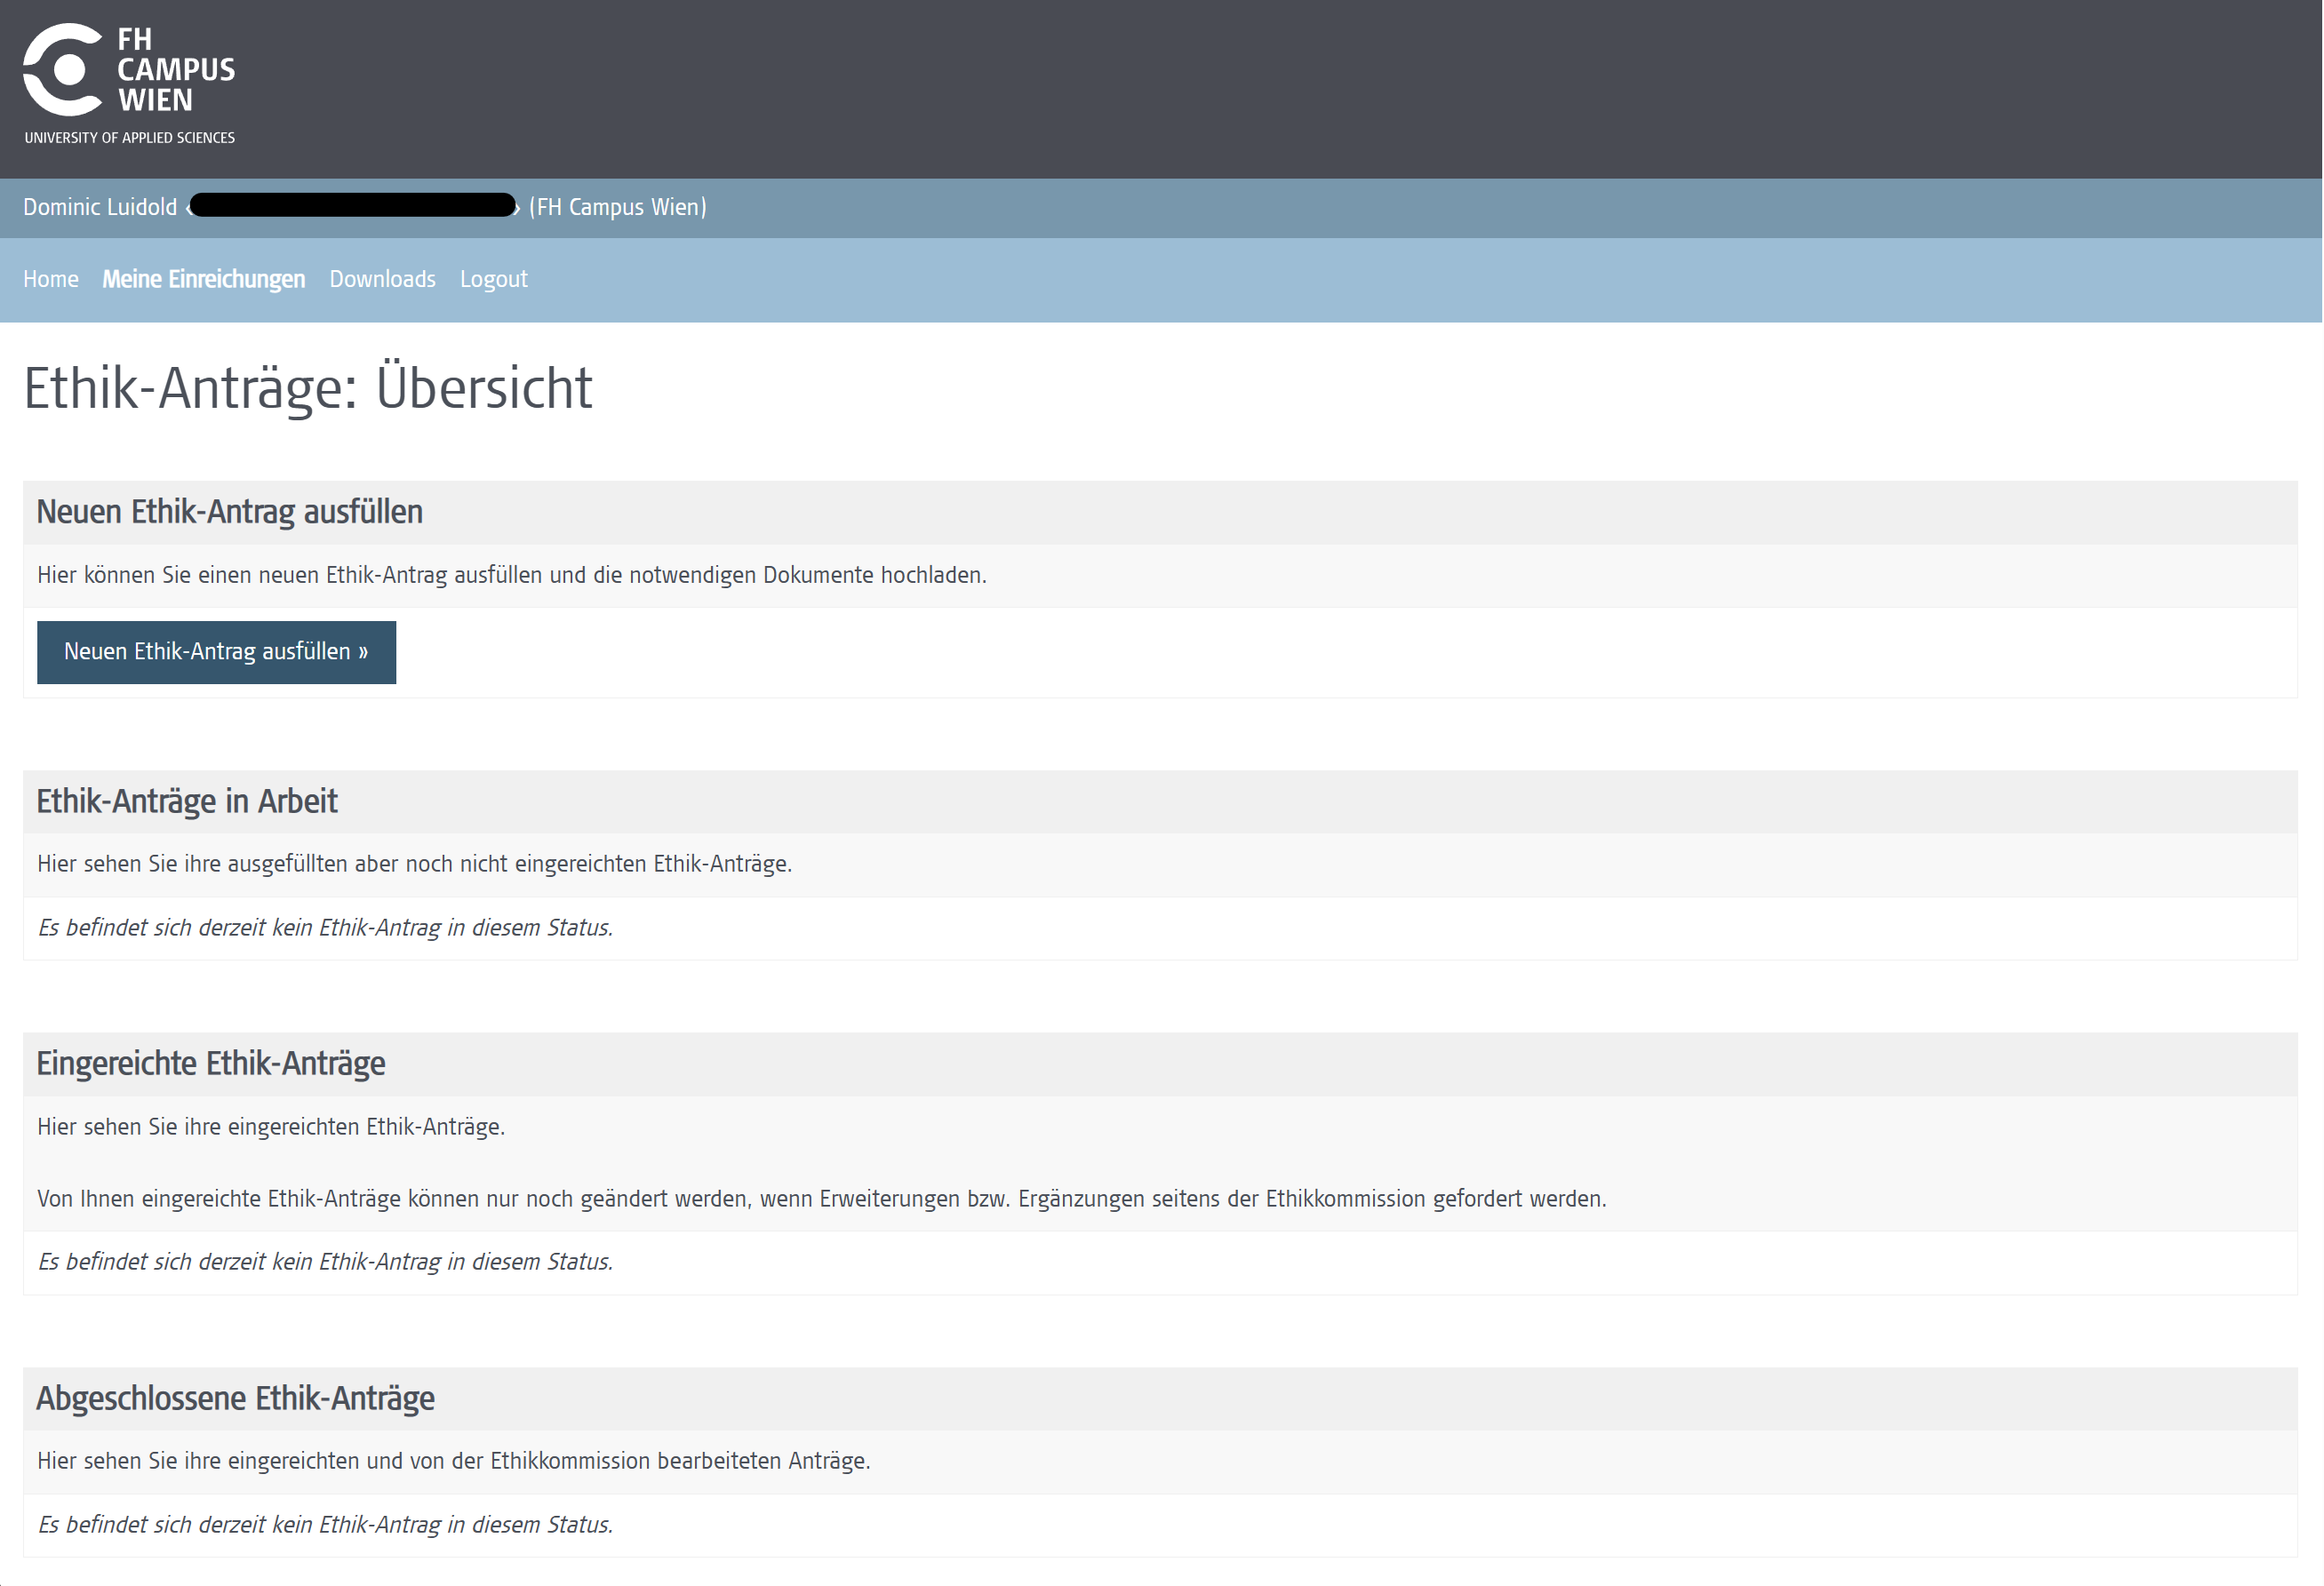
\includegraphics[width=\linewidth]{thesis/images/Luidold_Einreichplattform-FH-Campus-Wien.png}
    \caption[Startseite der Einreichplattform der FH Campus Wien im eingeloggten Zustand]{Startseite der Einreichplattform der FH Campus Wien im eingeloggten Zustand \cite{ethikkommission_fh_campus_wien_fh_2023}}
    \label{fig:startseite-einreichplattform-fhcw}
\end{figure}

\medskip 

Die Erstellung und Einreichung von Ethikanträgen basiert im genannten System auf mehreren Formularmasken, die Freitextfelder, Kontrollkästchen und Dropdown-Elemente enthalten. Der konkrete Antrag ist im Formular dabei in acht verschiedene Schritte unterteilt, die Fragen zu insgesamt fünf Themenblöcke stellen und Angaben von den Forschenden einholen. Zwischen den einzelnen Schritten kann jederzeit frei navigiert werden, wobei eine Zwischenspeicherung bei jedem Abschnittswechsel automatisch erfolgt. Abbildung \ref{fig:einreichplattform-fhcw-schritt-1-7} auf Seite \pageref{fig:einreichplattform-fhcw-schritt-1-7} zeigt Schritte 1 und 7, bei denen allgemeine Angaben zum Ethikantrag gemacht und sowohl verpflichtende als auch optionale Dokumente hochgeladen werden können. Schritt 8 dient der Zusammenfassung und abschließenden Kontrolle der bereitgestellten Daten, bei der alle Pflichtfelder auf Vollständigkeit überprüft und fehlende Felder entsprechend gekennzeichnet werden.

\begin{figure}[htp]
    \centering
    \begin{minipage}[t]{.99\linewidth}
        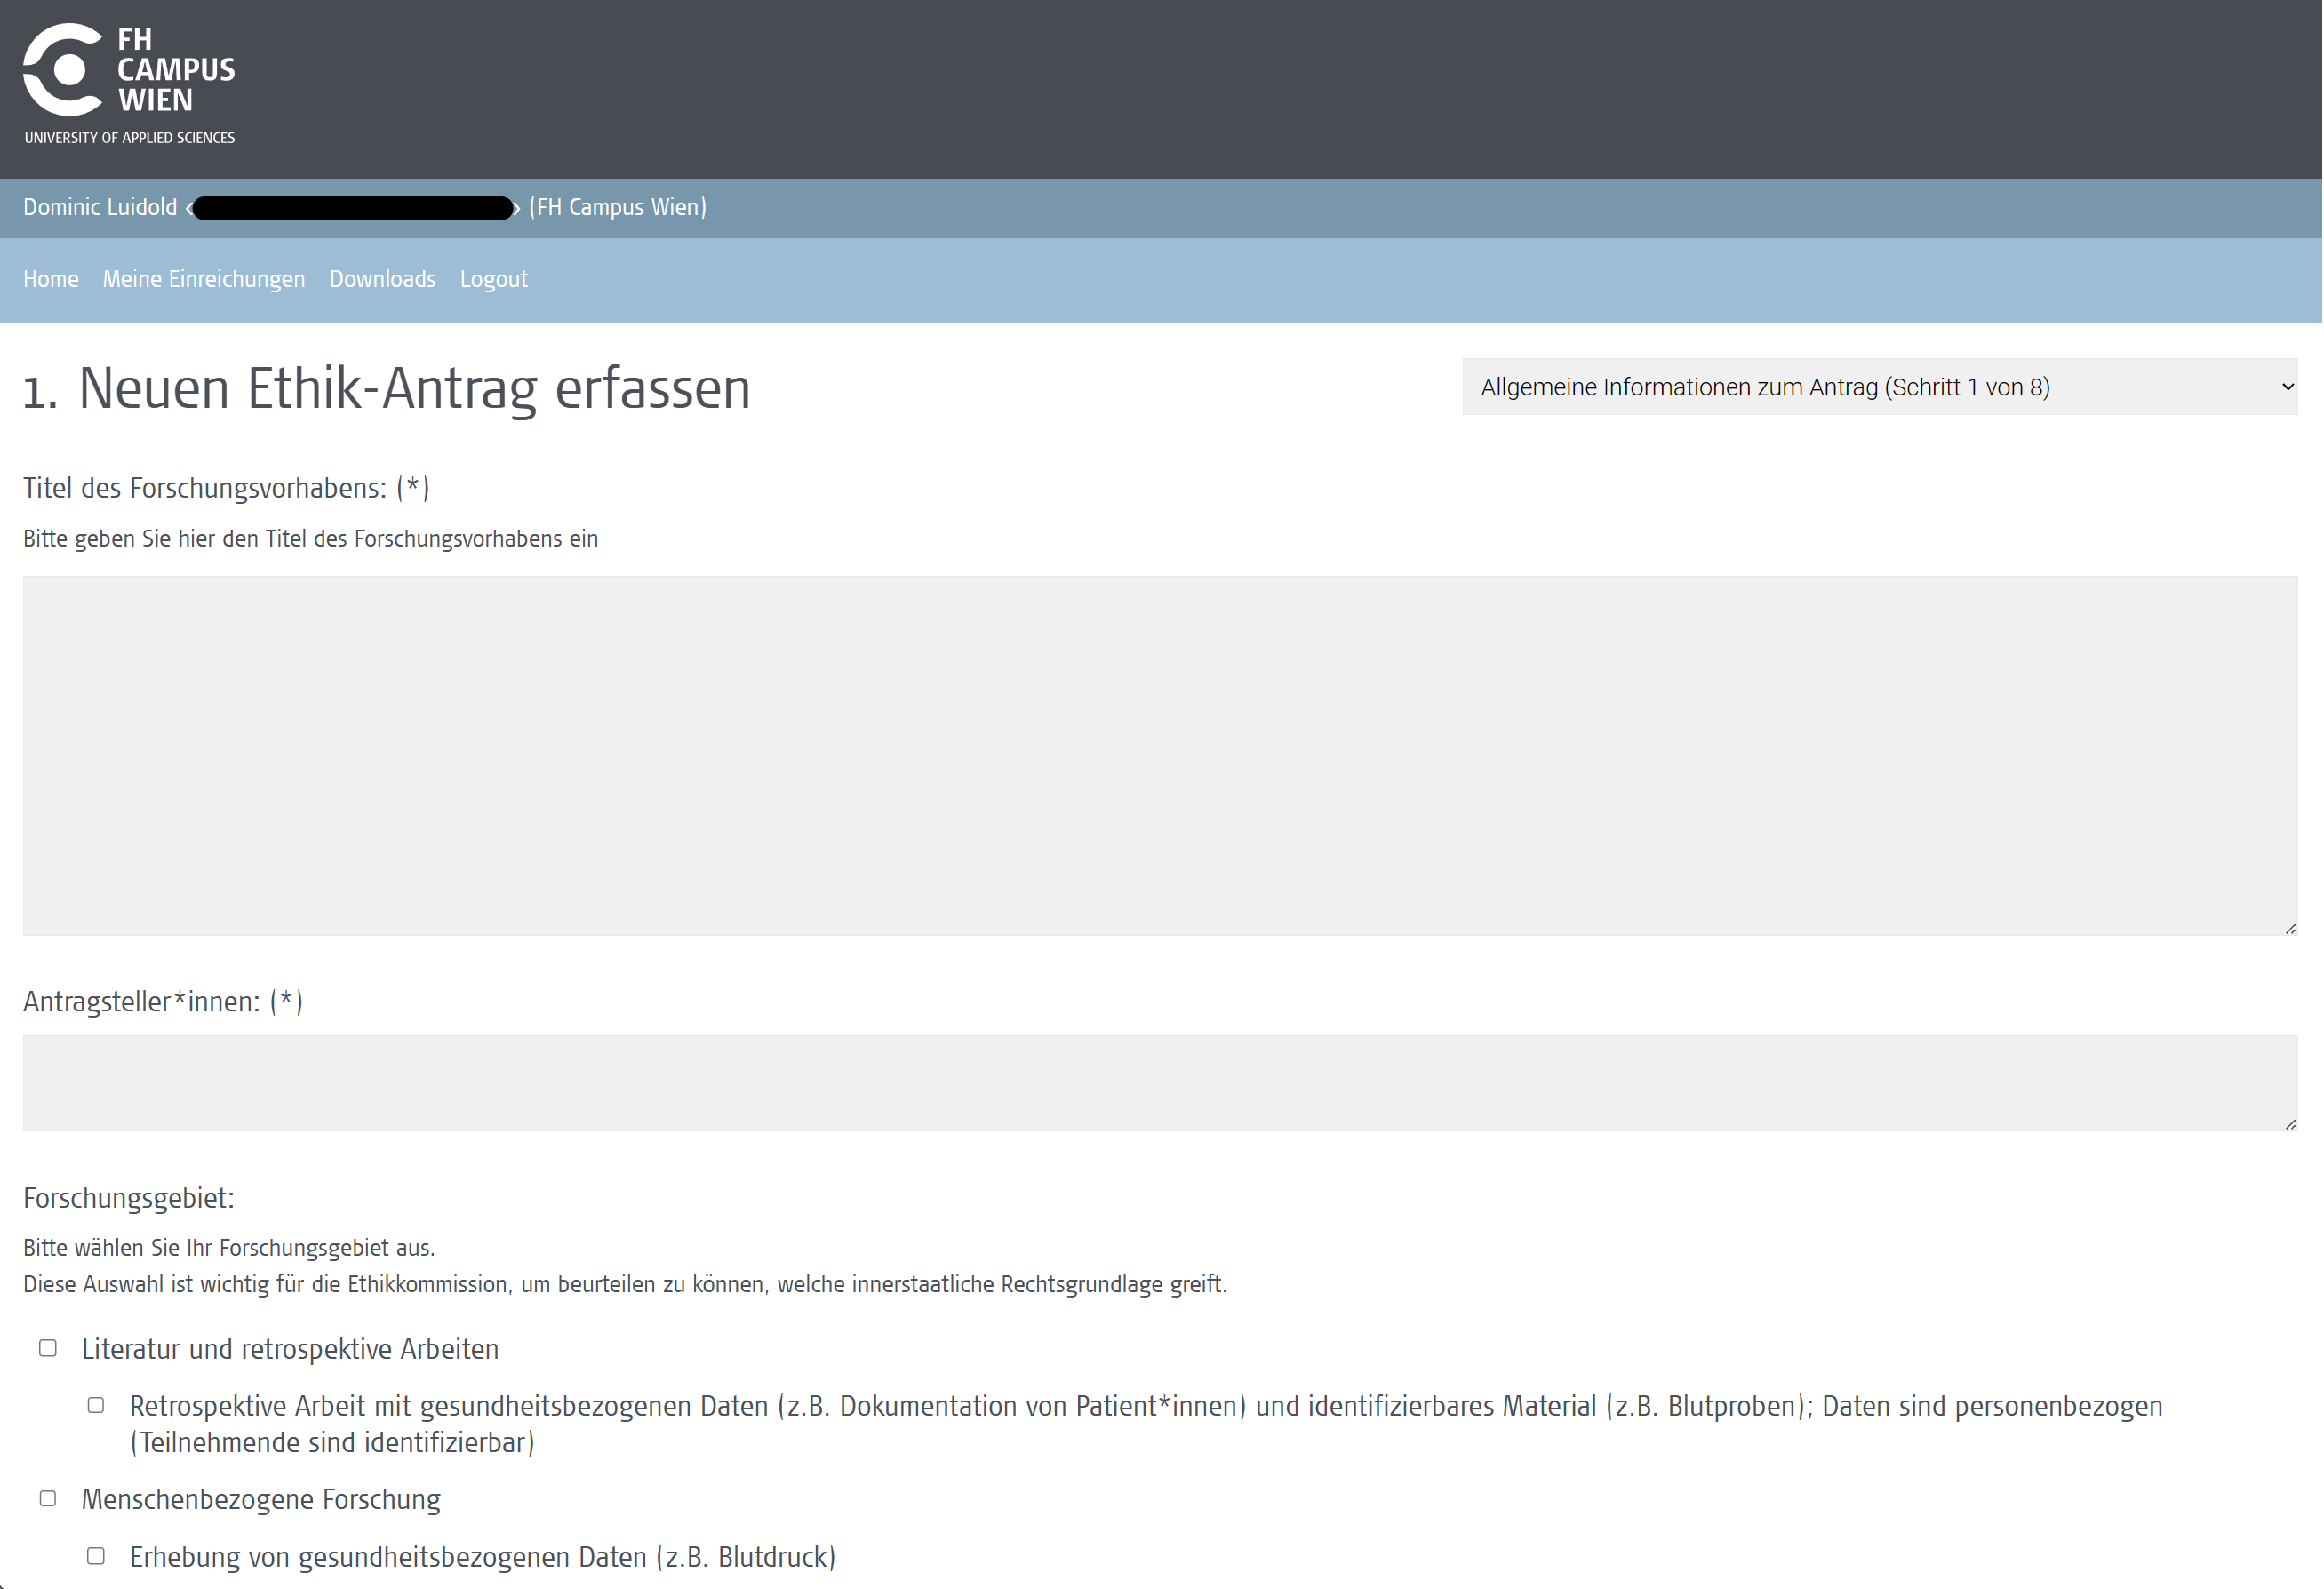
\includegraphics[width=\linewidth]{thesis/images/Luidold_Einreichplattform-Formular-Schritt-1.png}
    \end{minipage}
    \begin{minipage}[b]{.99\linewidth}
        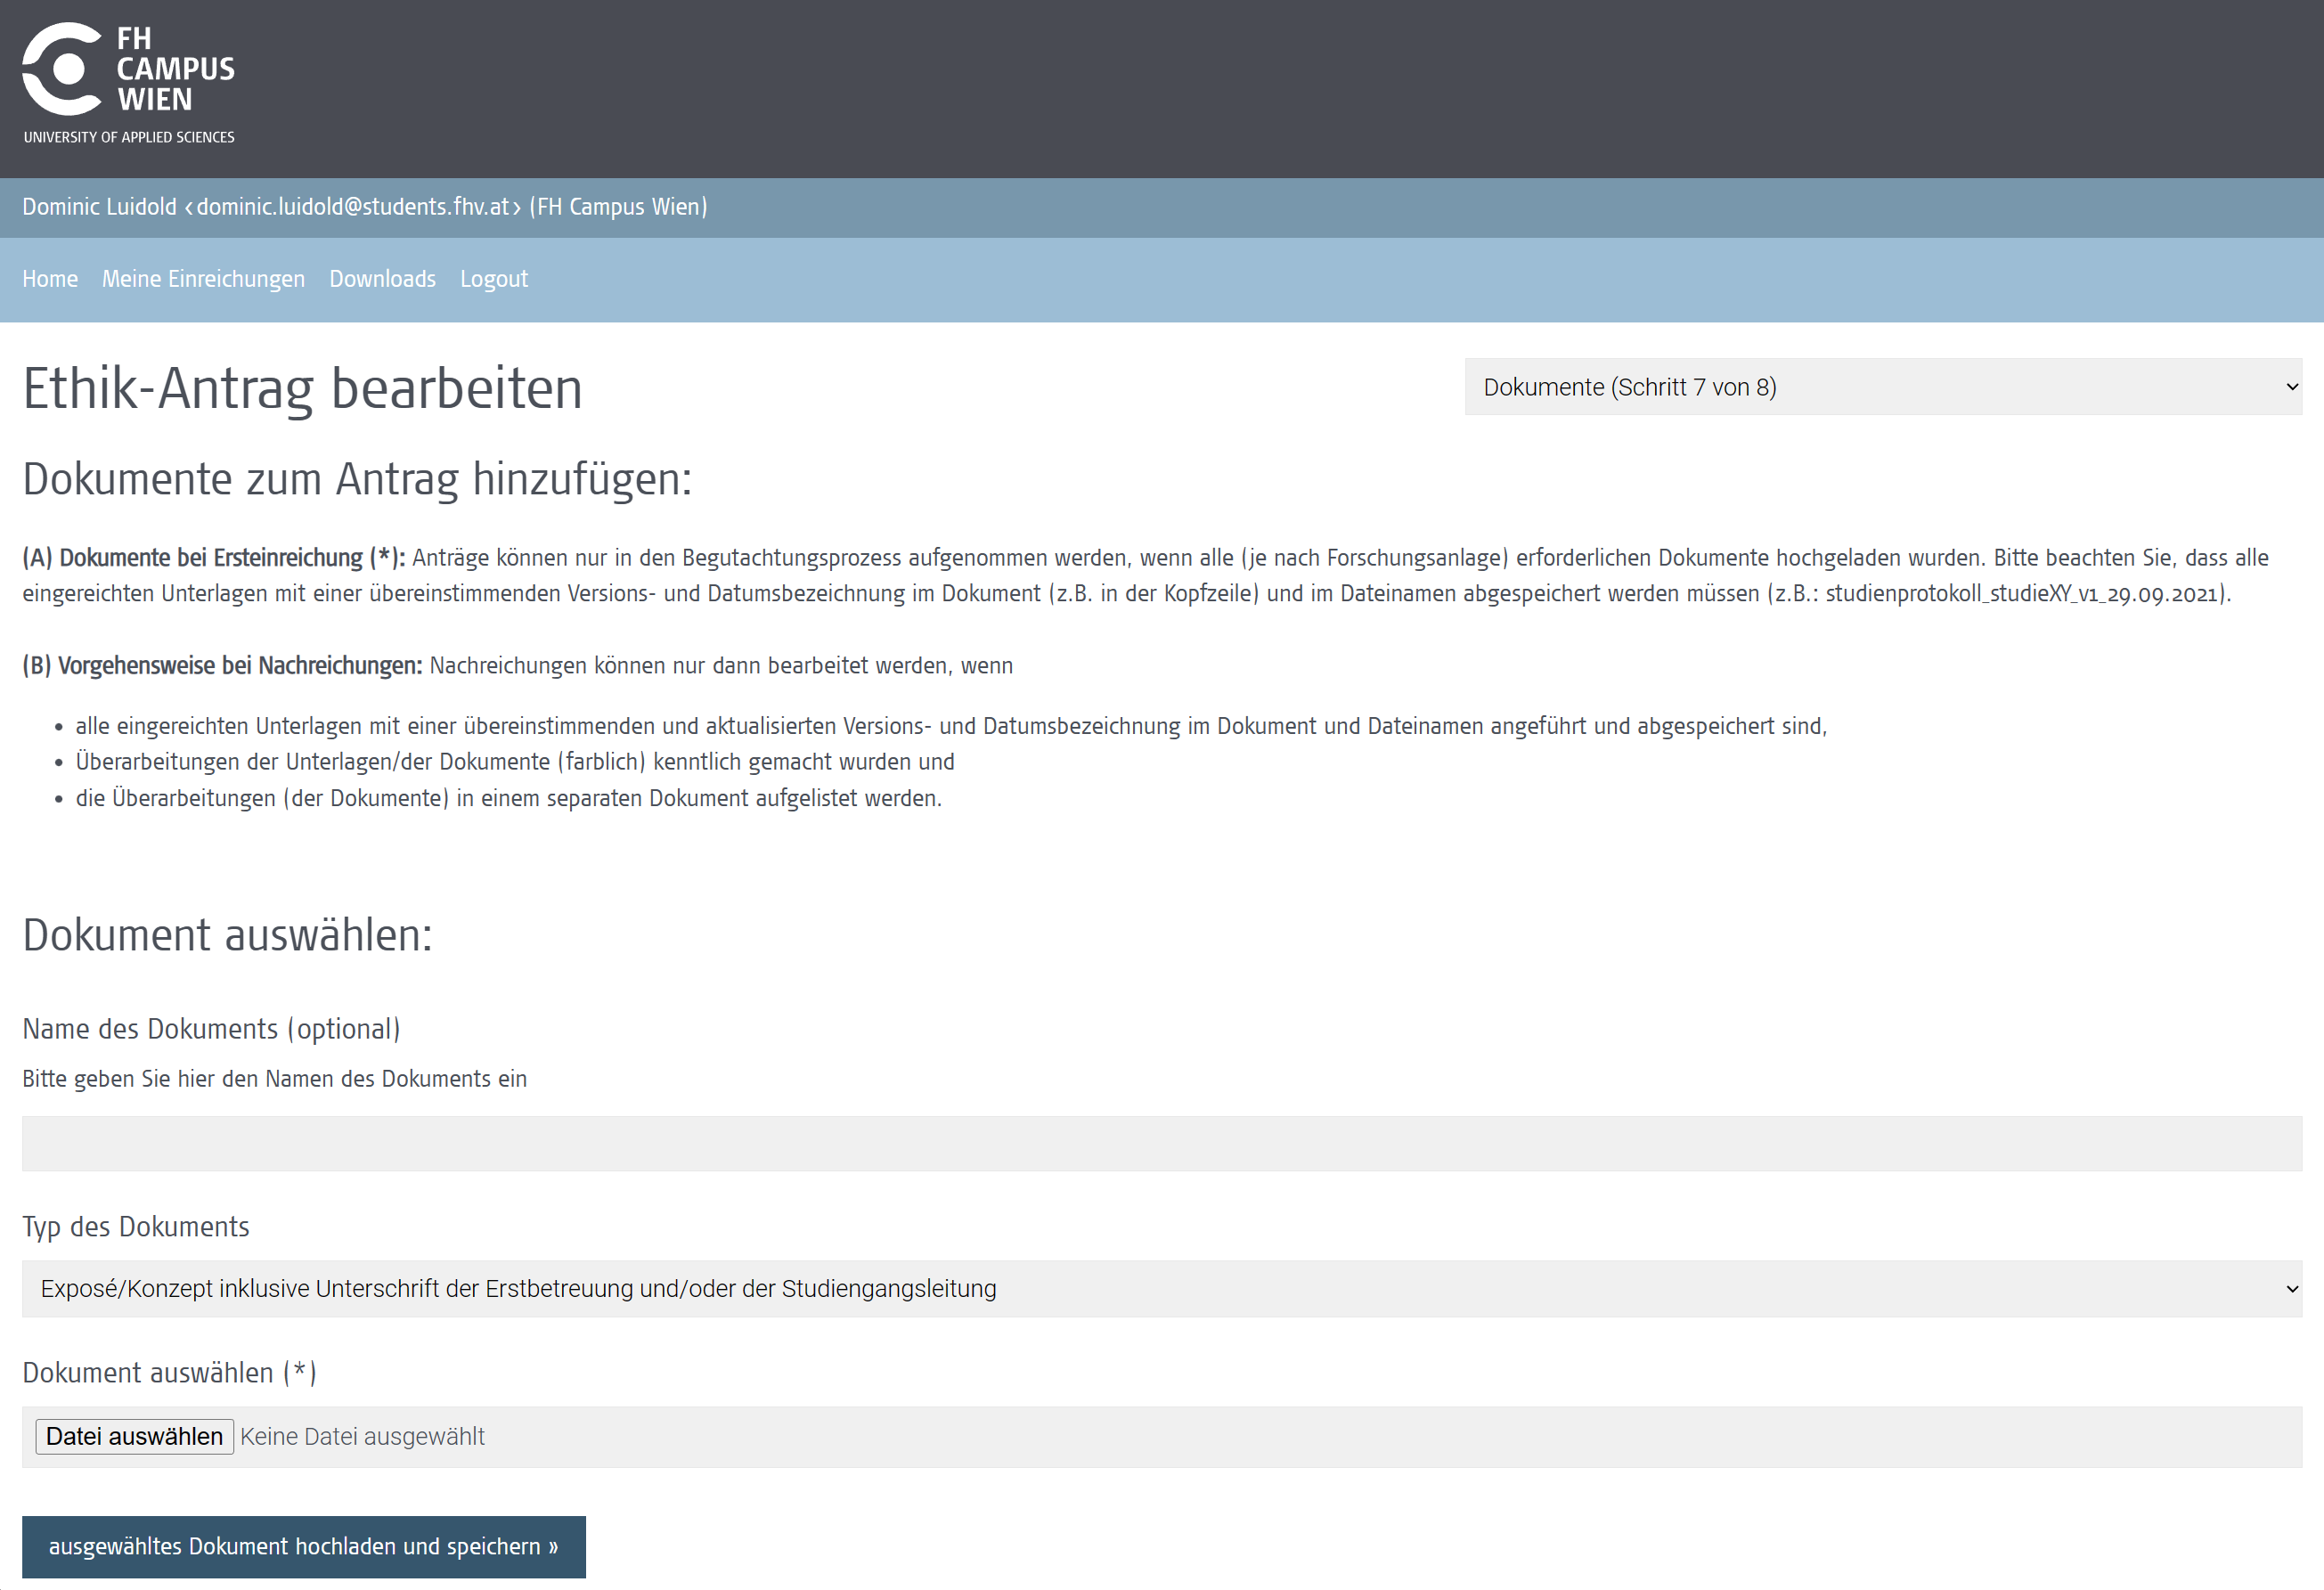
\includegraphics[width=\linewidth]{thesis/images/Luidold_Einreichplattform-Formular-Schritt-2.png}
    \end{minipage}
    \caption[Schritt 1 und Schritt 7 der Erstellung eines Ethikantrages mittels der Einreichplattform der FH Campus Wien]{Schritt 1 (oben) und Schritt 7 (unten) der Erstellung eines Ethikantrages mittels der Einreichplattform der FH Campus Wien \cite{ethikkommission_fh_campus_wien_fh_2023}}
    \label{fig:einreichplattform-fhcw-schritt-1-7}
\end{figure}

\medskip

Nach einer initialen Recherche und Begutachtung des über die Einreichplattform direkt einsehbaren Quellcodes im Browser konnten keine Anhaltspunkte dazu gefunden werden, wie die technische Umsetzung im Hintergrund der Einreichplattform aussieht und ob der gesamte Quellcode öffentlich zur Einsicht beziehungsweise zum Download zur Verfügung steht.

\subsubsection*{Inhaltlicher Aufbau}
\label{sub-sub-sec:fhcw-inhaltlicher-aufbau}

Inhaltlich ist der Antrag auf die bereits angesprochenen fünf Themenblöcke aufgeteilt, die die folgenden Bereiche abdecken:
\begin{itemize}
    \item \enquote{1. Allgemeine Daten zum Antrag},
    \item \enquote{2. Kurzdarstellung zum Forschungsvorhaben},
    \item \enquote{3. Forschungsethische Problemstellungen und Implikationen},
    \item \enquote{4. Datenschutz und rechtliche Aspekte} sowie
    \item \enquote{5. Dokumente}
\end{itemize}

\noindent wobei Themenblock 2 und 3 mit den jeweiligen Detailfragen im Antrag auf zwei separaten Seiten und Schritten auszufüllen sind.

Die einzelnen Themenblöcke enthalten Fragestellungen zur antragsstellenden Person, dem Forschungsvorhaben und -design sowie Fragen zur Risikoabschätzung und zum Datenschutz. In Themenblock 5 können zudem beliebig viele Dokumente hochgeladen werden, wobei die Formularmaske hierfür verschiedene Kategorien und Typen als mögliche Anhaltspunkte vorgibt.

\subsubsection*{Ähnlichkeiten \& Auffälligkeiten}
\label{sub-sub-sec:ähnlichkeiten-auffälligkeiten-fhcw}

Die Ethikkommission der FH Campus Wien nutzt den Download-Bereich der Einreichplattform, um neben den Hilfestellungen direkt in der Eingabemaske (siehe dazu Abbildung \ref{fig:einreichplattform-fhcw-schritt-1-7} auf Seite \pageref{fig:einreichplattform-fhcw-schritt-1-7}) weiterführende Informationen bereitstellen zu können. Die Ethikkommissionen bietet dort, unter anderem, ein Dokument zum Download an, welches einen Kriterienkatalog enthält, der aufzeigt, wann ein Ehtikantrag eingereicht werden muss und wann kein ethisches Votum erforderlich ist. Das Dokument beschreibt ebenso den Prozess der Antragsstellung sowie die erforderlichen und optionalen Angaben und Dokumente, die bereitgestellt werden können und müssen. Darüber hinaus informiert das Dokument über die möglichen Entscheidungen und Beschlussformen, die im Anschluss an die Antragsstellung zu erwarten sind. \cite[1\psqq]{ethikkommission_fh_campus_wien_wissenswertes_2022}

\medskip

Wie bereits in Abschnitt \ref{sub-sub-sec:möglichkeiten-funktionseinschränkungen} auf Seite \pageref{sub-sub-sec:möglichkeiten-funktionseinschränkungen} kurz erwähnt wurde, ist die Integration von Literaturverwaltungsprogrammen ein wichtiger Punkt für ein neues beziehungsweise erweitertes Ethikantragssystem der \acl{fek} der \acl{fhv}. Die Einreichplattform der FH Campus Wien empfiehlt in den oben erwähnten, weiterführenden Informationen für die Nutzung von Literaturverwaltungsprogrammen und die Verwaltung von Literaturlisten explizit die Dokumenten"=Anhangsfunktion in Schritt 7. \cite[5]{ethikkommission_fh_campus_wien_wissenswertes_2022}.

\medskip

Ähnlich zu der in Abschnitt \ref{sub-sub-sec:möglichkeiten-funktionseinschränkungen} auf Seite \pageref{sub-sub-sec:möglichkeiten-funktionseinschränkungen} hervorgehobenen Einschränkung der Word"=Antragsvorlage der \ac{fek} der \ac{fhv} bietet auch das Online-Portal keinerlei Möglichkeiten, Text zu formatieren oder gesondert hervorzuheben und fokussiert sich ausschließlich auf Zeichen und Zeichenlimits.

\medskip

Neben den bereits genannten Punkten ist bei der Analyse des Prozesses und des Online-Portals ersichtlich geworden, dass nicht eindeutig klar ist, wie die beworbene Zwischenspeicherung des Antrages durchgeführt werden kann, da das Formular und die Eingabemasken keinen dedizierten \enquote{Speichern}-Button enthalten. Wenn nach der Eingabe einer Information oder der Beantwortung einer Frage nicht der \enquote{Weiter}-Button am Ende des Formulars verwendet oder nicht über das Dropdown-Menü in der oberen rechten Ecke zu einem anderen Abschnitt gewechselt wird, erfolgt keine Speicherung und die Daten gehen verloren, sobald die Seite verlassen wird.

\subsubsection*{Schlussfolgerungen}
\label{sub-sub-sec:schlussfolgerungen-fhcw}

Die Einreichplattform der Ethikkommission der FH Campus Wien bietet in verschiedenen Bereichen Anhaltspunkte und Ideen, wie eine etwaiger Lösungsansatz im Rahmen dieser Masterarbeit aussehen könnte.

Unabhängig vom inhaltlichen Aspekt des Ethikantrages, der im Regelfall von der jeweiligen (Forschungs-)Ethikkommission bestimmt wird, sind vor allem das nahtlose Zwischenspeichern (trotz der Limitierungen) und freie Navigieren zwischen den einzelnen Abschnitten, das freie Hinzufügen und Hochladen von Dokumenten sowie der Fokus auf die wesentlichen Bestandteile entsprechende Anhaltspunkte. Der im Download-Bereich zur Verfügung gestellte Kriterienkatalog, um festlegen zu können, ob ein Ethikantrag notwenig ist, könnte ebenso Einfluss auf den den Lösungsansatz nehmen, da ähnliche Hilfestellungen auch in Abschnitt \ref{sub-sub-sec:kommunikation-email} auf Seite \pageref{sub-sub-sec:kommunikation-email} von Antragsteller:innen angesprochen wurden.

\subsection{Ethics Committee System}
\label{sub-sec:ecs}

Das \enquote{\ac{ecs}} beziehunsweise \enquote{Ethic Commission System} -- beide Namen werden mehrfach genannt -- wird von den Medizinischen Universitäten Wien, Innsbruck und Graz sowie weiterer Einrichtungen entwickelt und ist ein Webservice, der das Erstellen und Einreichen von Ethikanträgen zu klinischen Studien, den Votums-Prozess sowie das dazugehörige Antragswesen in einem System vereint. \cite{medizinische_universitat_wien_ecs-docs_about-2021}

\medskip

Das \ac{ecs} hat die Besonderheit, dass die Antragsstellung sich auf die in Abschnitt \ref{sub-sec:vorlage-föe} ab Seite \pageref{sub-sec:vorlage-föe} behandelten Antragsvorlage stützt und das Online auszufüllende Formular beinahe einer Eins-zu-Eins Umsetzung des Word-Dokumentes entspricht. Abbildung \ref{fig:abschnitt-sponsor-ecs} auf Seite \pageref{fig:abschnitt-sponsor-ecs} zeigt beispielhaft den Abschnitt \enquote{Sponsor}, der in der Word"=Dokumentenvorlage in Teil A ab Seite 1 zu finden ist. Auf der linken Seite der Abbildung lässt sich dabei gut erkennen, dass die einzelnen Formular-Felder mit einer Nummerierungen versehen sind, die mit der Nummerierung der Dokumentenvorlage des \ac{föe} übereinstimmen.

\begin{figure}[ht]
    \centering
    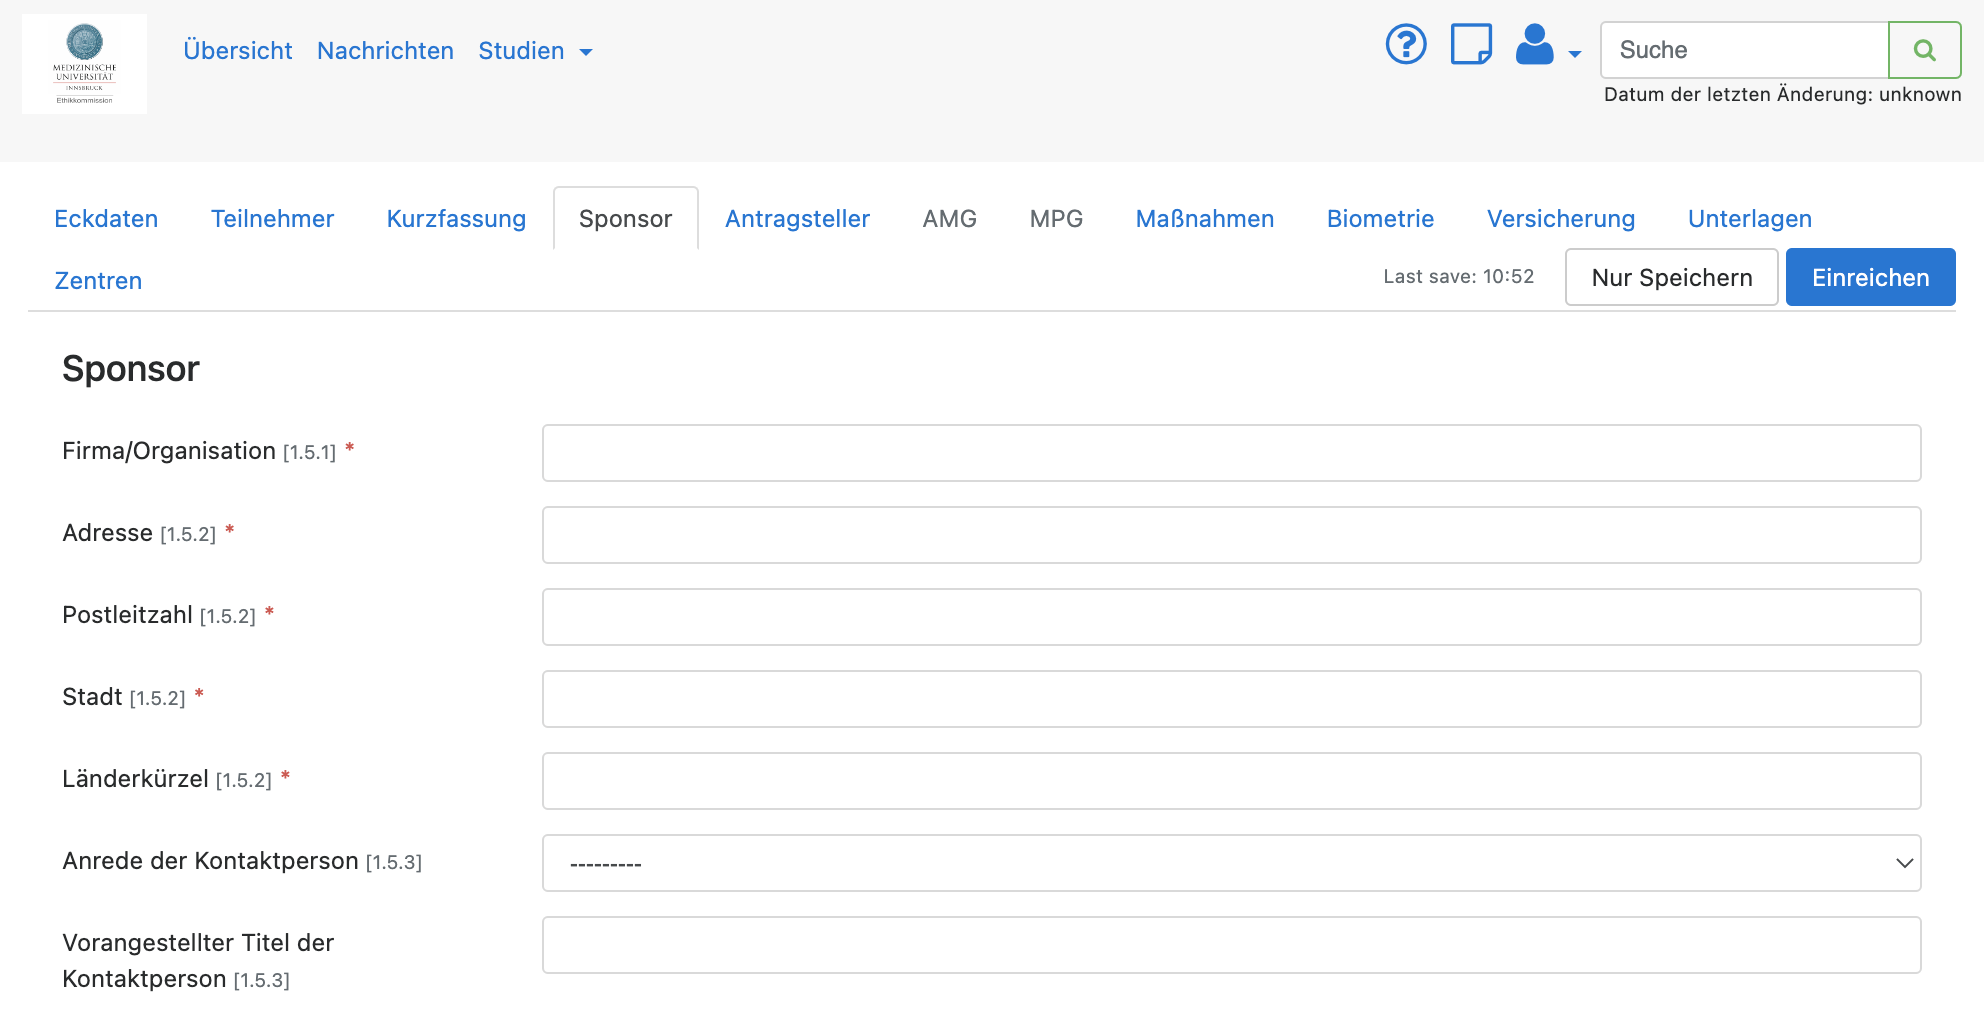
\includegraphics[width=\linewidth]{thesis/images/Luidold_ECS-Schritt-Eckdaten.png}
    \caption[Ausschnitt des Abschnittes \enquote{Sponsor} der Antragsstellung des \acl{ecs}]{Ausschnitt des Abschnittes \enquote{Sponsor} der Antragsstellung des \acl{ecs} \cite{ethikkommission_der_medizinischen_universitat_innsbruck_ethikkommission_2023}}
    \label{fig:abschnitt-sponsor-ecs}
\end{figure}

Die Ethikkommissionen der Medizinischen Universitäten Wien und Innsbruck akzeptieren Einreichungen von Ethikanträgen, trotz der Abhängigkeit und dem inhaltlichen Ursprung, nur noch mittels der jeweils eigenen \ac{ecs}-Instanz und nicht mehr mittels der Word"=Dokumentenvorlage des \ac{föe}. \cite{ethikkommission_der_medizinischen_universitat_wien_ethik_2023, medizinische_universitat_innsbruck_einreichungen_2023} Die Ethikkommission der Medizinischen Universität Graz verlinkt auf ihrer Website ebenso auf die eigene \ac{ecs}-Instanz, bittet zum Zeitpunkt dieser Arbeit jedoch um die Einreichung etwaiger Anträge über die Word"=Dokumentenvorlage des \ac{föe}, da es zu technischen Schwierigkeiten bei der Einreichung mittels dem \ac{ecs} kommt. \cite{medizinische_universitat_graz_ethikkommission_2023}

\subsubsection*{Technischer Aufbau}
\label{sub-sub-sec:ecs-technischer-aufbau}

Die Entwickler:innen des \acl{ecs} stellen, als einziges der in dieser Arbeit bisher analysierten Systeme auf Online-Basis, den Quellcode zur gesamten Applikation offen zur Verfügung\footnote{\ac{ecs} Quellcode online abrufbar auf GitHub (\url{https://github.com/ecs-org/ecs})} und bieten zusätzlich eine ausführliche Online-Dokumentation sowohl für die Nutzung als auch für die Entwicklung an. \cite{medizinische_universitat_wien_ecs-docs_about-2021, medizinische_universitat_wien_development_2021, medizinische_universitat_wien_installationusage_2021}

\medskip

Vergleichbar zur Einreichplattform der FH Campus Wien (siehe Abschnitt \ref{sub-sec:einreichplattform-fh-campus-wien} ab Seite \pageref{sub-sec:einreichplattform-fh-campus-wien}) basiert die Antragsstellung von Ethikanträgen, aus Sicht von Antragsteller:innen, aus mehreren Formular-Masken, die sowohl mit Freitext-Feldern, Kontrollkästchen als auch Dropdown-Elementen arbeiten und dabei in 12 verschiedene Kategorien beziehungsweise Unterpunkte aufgeteilt sind. Ebenfalls ähnlich zur Einreichplattform können dem Ethikantrag über den Unterpunkt \enquote{Unterlagen} im \ac{ecs} beliebig viele Dokumente und Unterlagen hinzugefügt werden, wobei auch hier verschiedene Kategorien und Typen als mögliche Anhaltspunkte bereitgestellt werden. Im Gegensatz zur Einreichplattform der FH Campus Wien findet jedoch keine automatische Speicherung der eingegebenen Daten und Informationen statt -- das (Zwischen-)Speicher der Daten erfolgt im \ac{ecs} über einen dedizierten Button im rechten oberen Bereich der Benutzeroberfläche. Das freie Wechseln zwischen den einzelnen Abschnitten ist während der Bearbeitung des Antrages dennoch möglich.

Wie in Abbildung \ref{fig:ecs-studien-nachrichten-notizen} auf Seite \pageref{fig:ecs-studien-nachrichten-notizen} zu sehen ist, bietet das \ac{ecs} den antragsstellenden Personen, neben der konkreten Möglichkeit zur Einreichung von Ethikantrage, zudem eine Nachrichten- sowie Notiz-Funktion an, die für den Erhalt von Informationen sowie zum erstellen persönlicher Notizen genutzt werden kann.

\begin{figure}[ht!]
    \centering
    \begin{minipage}[t]{.85\linewidth}
        \includegraphics[width=\linewidth]{thesis/images/Luidold_ECS-Studien-Überblick.png}
    \end{minipage}
    \begin{minipage}[b]{.85\linewidth}
        
\includegraphics[width=\linewidth]{thesis/images/Luidold_ECS-Nachrichten-Notizen.png}
    \end{minipage}
    \caption[Übersicht eingereichter und offener Studien (oben) sowie der Nachrichten- und Notizen-Funktion (unten) des \acl{ecs}]{Übersicht eingereichter und offener Studien sowie der Nachrichten- und Notizen-Funktion des \acl{ecs} \cite{ethikkommission_der_medizinischen_universitat_innsbruck_ethikkommission_2023}}
    \label{fig:ecs-studien-nachrichten-notizen}
\end{figure}

Das \acl{ecs} basiert dabei auf einer mittels Python\footnote{Python (\url{https://www.python.org/})} und dem dafür zur Verfügung stehenden Webframework Django\footnote{Django Webframework (\url{https://www.djangoproject.com/})} umgesetzten Webapplikation, welche die Applikationsdaten in einer mit dem PostgreSQL\footnote{PostgreSQL (\url{https://www.postgresql.org/)}} \ac{dbms} verwalteten Datenbank ablegt. Die Webapplikation beziehungsweise die Python-Umgebung läuft dabei auf einem Ubuntu Xenial Cloud Image\footnote{Ubuntu 16.04 LTS (Xenial Xerus) (\url{https://cloud-images.ubuntu.com/releases/server/xenial/release/})} der Version \texttt{16.04 LTS}. Das \ac{ecs} bedient sich zusätzlich weiterer Technologien, um die gesamte Anwendung (und auch die Anwendungsfälle, die in dieser Analyse außen vor gelassen werden) anbieten zu können. In Abbildung \ref{fig:ecs-service-architektur} auf Seite \pageref{fig:ecs-service-architektur} ist ersichtlich, welche weiteren Technologien, Frameworks und Services zum Einsatz kommen und die Abbildung gibt gleichzeitig auch ein Überblick über die Service-Architektur der gesamten Web-Applikation. \cite{medizinische_universitat_wien_ecs-docs_about-2021, medizinische_universitat_wien_ecs-handbook_development-2021}

\begin{figure}[ht]
    \centering
    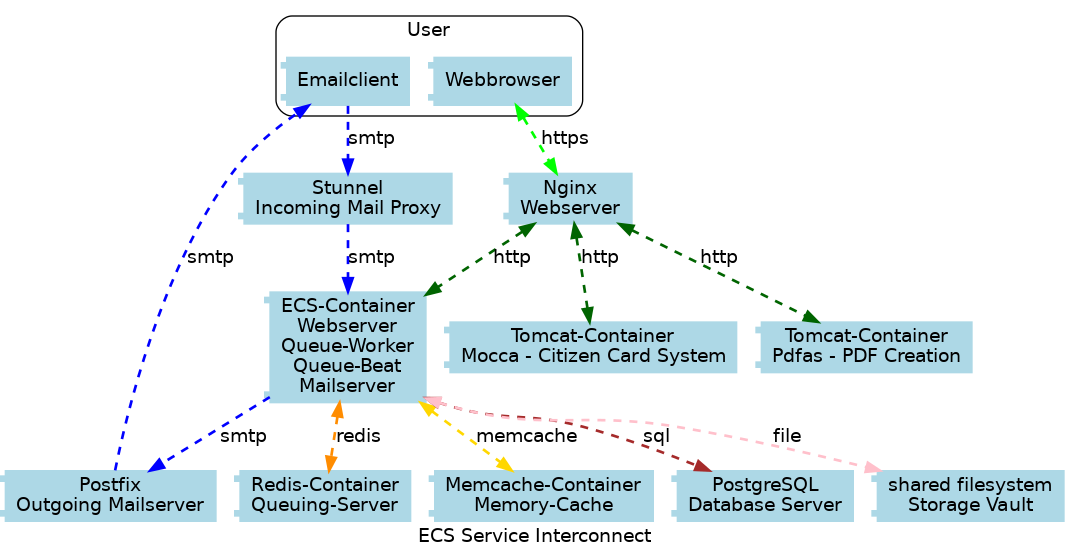
\includegraphics[width=\linewidth]{thesis/images/ECS_Service-Architecture.png}
    \caption[Übersicht verwendeter Technologien und Frameworks sowie der Service-Architektur des \acl{ecs}]{Übersicht verwendeter Technologien und Frameworks sowie der Service-Architektur des \acl{ecs} \cite{medizinische_universitat_wien_ecs-handbook_development-2021}}
    \label{fig:ecs-service-architektur}
\end{figure}

Das eingesetzte Django Framework ist laut Definition der Django Software Foundation mittels einer \ac{mvt} Architektur umgesetzt, die bei genauerer Betrachtung auch einer \ac{mvc} Architektur zugeordnet werden kann. In beiden Architektur-Ansätzen gibt es sowohl ein sogenanntes \texttt{Model}, während Djangos \texttt{Template} dem \texttt{View} der \ac{mvc}-Architektur und Djangos \texttt{View} dem \texttt{Controller} der \ac{mvc}-Architektur entspricht beziehungsweise zugeordnet werden kann. Die unterschiedliche Namensgebung der einzelnen Komponenten geht dabei auf die Auffassung zurück, dass die \texttt{View} nicht entscheidet, \textit{wie} Daten aussehen, sondern \textit{welche} Daten zur Verfügung gestellt werden, während das \texttt{Template} entscheidet, \textit{wie} die Daten präsentiert werden. Der \texttt{Controller} ist laut der Foundation das Framework selbst. \cite{django_software_foundation_faq_2023}

\medskip

Django ist als \ac{mvt}/\ac{mvc}-Framework darauf ausgelegt, sowohl für die Domänen- und Applikationslogik im für Antragsteller:innen nicht sichtbaren Teil der Applikation (sprich dem \texttt{Model} und dem \texttt{Controller} im Sinne von \ac{mvc}) als auch für das direkt im Browser sichtbare \ac{ui} (sprich dem \texttt{View} im Sinne von \ac{mvc}) genutzt zu werden, wovon das \ac{ecs} nach grundlegender Durchsicht des Quellcodes entsprechend auch Gebrauch macht. \cite{ethics_commission_system_organization_ecs_2021}

\subsubsection*{Inhaltlicher Aufbau}
\label{sub-sub-sec:ecs-inhaltlicher-aufbau}

Da das \ac{ecs} sich an den vom \acl{föe} herausgegebenen Antrag sowohl inhaltlich als auch strukturell orientiert, entfällt an dieser Stelle eine erneute Analyse zum inhaltlichen Aufbau. Weiterführende Informationen können diesbezüglich in Abschnitt \ref{sub-sub-sec:föe-inhaltlicher-aufbau} ab Seite \pageref{sub-sub-sec:föe-inhaltlicher-aufbau} entnommen werden.

\subsubsection*{Ähnlichkeiten \& Auffälligkeiten}
\label{sub-sub-sec:ähnlichkeiten-auffälligkeiten-ecs}

Das \acl{ecs} verfügt als \ac{oss} über eine sehr ausführliche und detailreiche Dokumentation (siehe dazu \cite{medizinische_universitat_wien_ecs-docs_about-2021, medizinische_universitat_wien_development_2021, medizinische_universitat_wien_installationusage_2021, medizinische_universitat_wien_ecs-handbook_development-2021, ethics_commission_system_organization_ecs_2021}), sowohl für die Nutzung aus Sicht als Antragsteller:in beziehungsweise Verwalter:in des Systems als auch für Entwickler:innen, die die Applikation potenziell weiterentwickeln oder betreuen möchten. Diese Hilfestellungen stehen dabei nicht nur über das Entwicklerportal zur Verfügung, sondern werden auch direkt in den jeweiligen Instanzen des Systems verlinkt und Benutzer:innen als Hilfestellung angeboten.\footnote{Siehe beispielsweise die \ac{ecs}-Instanz der Ethikkommission der Medizinischen Universität Innsbruck: \url{https://ek-mui-tirol.at/help/}}

\medskip

Ähnlich zu der in Abschnitt \ref{sub-sub-sec:möglichkeiten-funktionseinschränkungen} auf Seite \pageref{sub-sub-sec:möglichkeiten-funktionseinschränkungen} hervorgehobenen Einschränkung der Word"=Antragsvorlage der \ac{fek} der \ac{fhv} und auch zur in Abschnitt \ref{sub-sec:einreichplattform-fh-campus-wien} ab Seite \pageref{sub-sec:einreichplattform-fh-campus-wien} analysierten Einreichplattform der FH Campus Wien bietet das \acl{ecs} keinerlei Möglichkeiten, Text zu formatieren oder gesondert hervorzuheben und fokussiert sich ausschließlich auf Zeichen und Zeichenlimits.

\medskip

Unabhängig von den bereits genannten Punkten nutzt das \ac{ecs} auch die individuellen Formular-Masken, um während der Antragsstellung zusätzliche Informationen und Hilfestellungen bereitzustellen. Diese sollen die Antragsteller:innen sowohl bei der Bearbeitung unterstützen als auch weiterführende Informationen liefern. Dabei werden sowohl Texte angezeigt, die sich direkt auf bestimmte Formularfelder beziehen, als auch allgemeine Hinweise in Form eines Banners am Anfang eines Formulars. Ein Beispiel hierfür ist in Abbildung \ref{fig:ecs-banner-hilfestellung} auf Seite \pageref{fig:ecs-banner-hilfestellung} dargestellt.

\begin{figure}[ht]
    \centering
    
\includegraphics[width=\linewidth]{thesis/images/Luidold_ECS-Banner-Hilfestellung.png}
    \caption[Hilfestellung in Form eines Banners im \acl{ecs}]{Hilfestellung in Form eines Banners im \acl{ecs} \cite{ethikkommission_der_medizinischen_universitat_innsbruck_ethikkommission_2023}}
    \label{fig:ecs-banner-hilfestellung}
\end{figure}

\subsubsection*{Schlussfolgerungen}
\label{sub-sub-sec:schlussfolgerungen-ecs}

Zwar bietet das \acl{ecs} als gesamte Applikation deutlich mehr Funktionalitäten als die ursprüngliche Word"=Antragsvorlage des \ac{föe} und geht über die reine Antragsstellung hinaus, die Erstellung eines Antrages selbst entspricht jedoch einer beinahe Eins-zu-Eins Umsetzung. Im zu erarbeitenden Lösungsansatz dieser Masterarbeit soll, wie in Abschnitt \ref{sec:frage-problemstellung} ab Seite \pageref{sec:frage-problemstellung} erwähnt, eine tiefere Einarbietung in etwaige Lösungsansätze erfolgen.

Nichtsdestotrotz bietet das \ac{ecs}, welches von verschiedenen Ethikkommissionen verwendet wird und gewisse Ähnlichkeiten zur Einreichplattform der FH Campus Wien hat, in einigen Bereichen Anhaltspunkte und Ideen, die in die Umsetzung des Lösungsansatzes dieser Masterarbeit einfließen könnten. Die zusätzliche Bereitstellung von Informationen über farbliche gekennzeichnete Banner, ein klares und verständliches Konzept des (Zwischen-)Speicherns bei freier Navigation und womöglich auch der Verweis auf externe Anleitungen und Hilfestellungen der Ethikkommission zählen, unter anderem, dazu.

\section{Systeme ohne konkreten Bezug}
\label{sec:systeme-ohne-bezug}

Die Anforderungen an eine Neuentwicklung des Ethikantrag-Tools der \ac{fek} der \ac{fhv} werden zwar erst in Kapitel \ref{chap:anforderung-neues-system} ab Seite \pageref{chap:anforderung-neues-system} definiert, jedoch ist bereits im Vorfeld ersichtlich, dass der Datenschutz sowie die Anpassungs- und Erweiterungsmöglichkeiten bei der potenziellen Auswahl anderer Systeme eine wichtige Rolle spielen. Dies ergibt sich sowohl aus dem Prozess als auch aus den von den Antragsteller:innen bereitgestellten Daten, mit denen die \acl{fek} arbeitet. Die nachfolgend analysierten Systeme werden daher vor allem auf diese Aspekte hin beleuchtet, neben den Möglichkeiten, die diese unabhängig davon bieten.

\subsection{\aclp{cms}}
\label{sub-sec:cms-syteme}

\acp{cms} wie beispielsweise WordPress\footnote{WordPress (\url{https://wordpress.org/})}, Joomla!\footnote{Joomla! (\url{https://www.joomla.de/})} oder TYPO3\footnote{TYPO3 \url{https://typo3.org/}} bieten grundlegend eine Vielzahl an Möglichkeiten, eigene Inhalte zu erstellen, zu editieren und auf einer Website zu veröffentlichen sowie eigene Workflows abzubilden. \cite{oracle_corporation_who_2022} Alle der drei genannten Systeme können dabei mit Plugins beziehungsweise Extensions erweitert werden, um Funktionen, die nicht standardmäßig enthalten sind, nachträglich hinzufügen zu können.\footnote{WordPress nennt diese Erweiterungen \enquote{Plugins} (siehe \url{https://wordpress.org/plugins/}) während Jommla! und TYPO3 diese Erweiterungen \enquote{Extensions} nennt (siehe \url{https://extensions.joomla.org/} sowie \url{https://extensions.typo3.org/}).}

\medskip

Von den drei genannten \aclp{cms}n hat WordPress den höchsten Marktanteil mit über 63\% an Websites, die mittels eines \ac{cms} betrieben werden und einen Marktanteil von insgesamt über 43\% aller Websites, die von \cite{q-success_di_gelbmann_gmbh_usage_2023} analysiert wurden. Die nachfolgende Analyse von etwaigen Möglichkeiten zur Umsetzung eines Ethikantrag-Tools fokussiert sich daher auf den Marktführer, für den es -- laut eigenen Angaben \cite{wordpress_foundation_wordpress_2023} -- über 60.000 kostenlose Plugins im offiziellen Verzeichnis gibt.

\subsubsection*{WordPress}
\label{sub-sub-sec:wordpress}

WordPress unterstützt die Erstellung von Formularen beziehungsweise ähnlicher Workflows nicht von Haus aus. Dank der Vielzahl an zur Verfügung stehenden Plugins kann diese Funktionalität jedoch nachträglich zum Funktionsumfang hinzugefügt werden.

Die grundlegende Erstellung einer Eins-zu-Eins Umsetzung der bestehenden Word"=Antragsvorlage der \ac{fek} der \ac{fhv} ließe sich mit einem entsprechenden Formular-Plugin umsetzen. Nach kurzer Recherche liefert \cite{morris_8_2023} eine Liste von sowohl kostenlosen als auch kostenpflichtigen Erweiterungen, die sich dafür eignen könnten:
\begin{itemize}
    \item Formidable Forms\footnote{Formidable Forms (\url{https://formidableforms.com/})}
    \item Gravity Forms\footnote{Gravity Forms (\url{https://www.gravityforms.com/})}
    \item Ninja Forms\footnote{Ninja Forms (\url{https://ninjaforms.com/})}
    \item WPForms\footnote{WPForms (\url{https://wpforms.com/})}
    \item ...\footnote{Siehe \cite{morris_8_2023} für eine vollständige Aufzählung inklusive detaillierterer Informationen der von Morris genannten Erweiterungsmöglichkeiten.}
\end{itemize}

Die weiterführende Antragsverwaltung und der Votums-Prozess laut der Verfahrensordnung der \ac{fek} (siehe \cite{forschungsethik-kommission_der_fachhochschule_vorarlberg_verfahrensordnung_2020}) können mit den genannten Erweiterungen jedoch nur teilweise abgebildet werden. Im weiteren Verlauf wäre eine entsprechende Analyse der in Kapitel \ref{chap:anforderung-neues-system} ab Seite \pageref{chap:anforderung-neues-system} gestellten Anforderungen notwendig, um festzumachen, in wie weit die von den Plugins bereitgestellten Formular-Masken und weitere Schritte potenziell davon betroffen sein könnten. Unabhängig davon kann WordPress ohne großen Aufwand selbständig heruntergeladen und installiert werden, wobei der dafür benötigte Speicherort -- beispielsweise ein Server der \acl{fhv} -- und die Zugangsberechtigungen selbstständig gewählt und verwaltet werden können.

\subsection{Online Formular-Tools}
\label{sub-sec:formular-tools}

Neben den gängigen \acp{cms}-Lösungen gibt es sowohl von Google als auch Microsoft und anderen Anbietern Online Formular-Tools, mit denen theoretisch ebenso eine Eins-zu-Eins Umsetzung der Word"=Antragsvorlage möglich ist. Abbildung \ref{fig:microsoft-google-forms-testformulare} auf Seite \pageref{fig:microsoft-google-forms-testformulare} zeigt zwei Test-Formulare, welche Beispielhaft mit Microsoft Forms\footnote{Microsoft Forms (\url{https://www.microsoft.com/de-de/microsoft-365/online-surveys-polls-quizzes})} und mittels Google Forms\footnote{Google Forms (\url{https://www.google.com/forms/about/})} umgesetzt wurden.

\begin{figure}[ht]
    \centering
    \begin{minipage}{.49\textwidth}
        \centering
        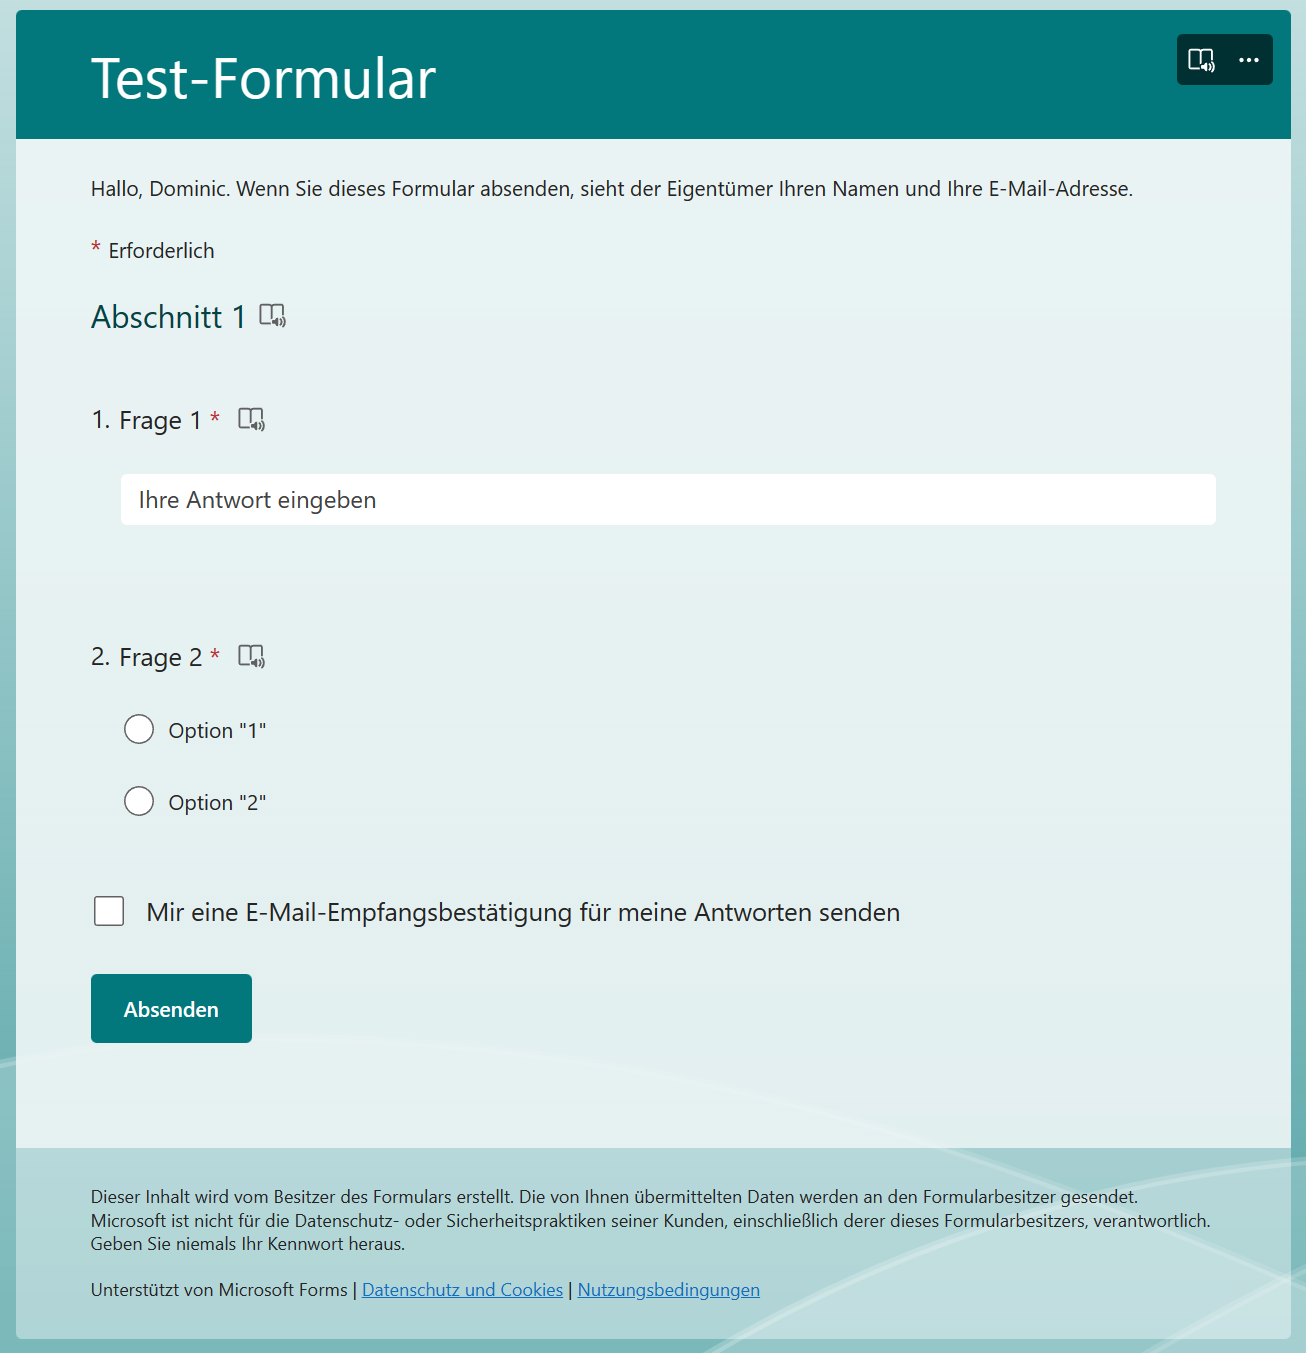
\includegraphics[width=.95\linewidth]{thesis/images/Luidold_Microsoft-Forms-Testformular.png}
    \end{minipage}
    \begin{minipage}{.49\textwidth}
        \centering
        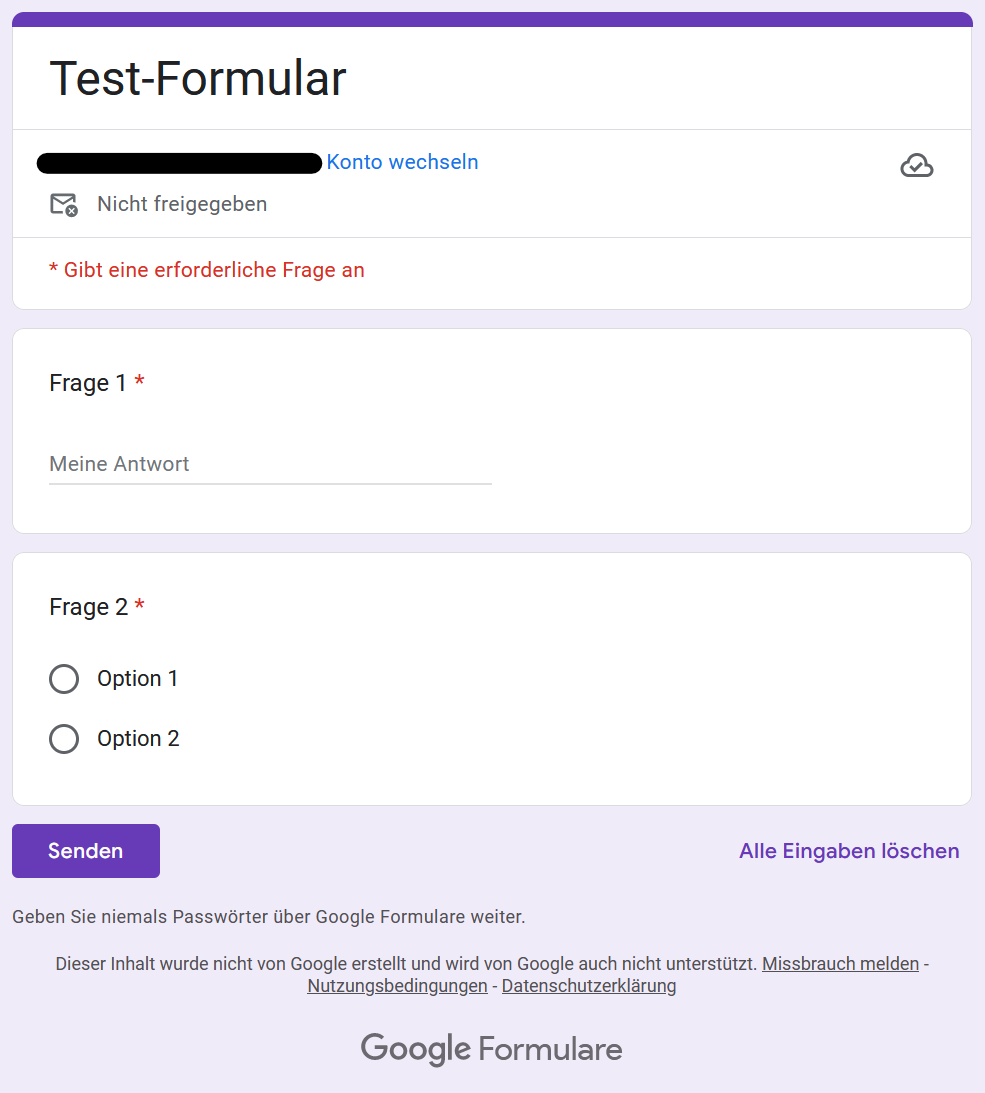
\includegraphics[width=.95\linewidth]{thesis/images/Luidold_Google-Forms-Testformular.png}
    \end{minipage}
    \caption[Test-Formulare umgesetzt mit Microsoft Forms und Google Forms]{Test-Formulare umgesetzt mit Microsoft Forms (links) und Google Forms (rechts) (Quelle: eigene Abbildungen)}
    \label{fig:microsoft-google-forms-testformulare}
\end{figure}

Ähnlich zu den in Abschnitt \ref{sub-sec:cms-syteme} ab Seite \pageref{sub-sec:cms-syteme} behandelten \aclp{cms} stellt sich die weiterführende Umsetzung als schwierig beziehungsweise nicht möglich dar, wenn sowohl die für den Prozess notwendigen als auch die von den Antragsteller:innen sowie der \ac{fek} gewünschten Funktionalitäten umgesetzt werden sollen. Eingelangte Antworten werden bei beiden Tools aggregiert gesammelt und können lediglich als Excel-Datei exportiert und von dort aus weiter bearbeitet werden. \cite{microsoft_corporation_wie_2021, google_ireland_limited_ergebnisse_2023} Unabhängig davon stellt sich bei beiden Tools die Frage, in wie weit die hohen Anforderungen der \acl{fek} an den Datenschutz erfüllt werden können, da die schlussendliche Datenspeicherung bei den jeweiligen Tools -- in diesem Fall Microsoft beziehungsweise Google -- liegt und keine direkte Kontrolle möglich ist.\footnote{\cite{visitor_analytics_gmbh_ist_2022} erklärt in diesem Zusammenhang, dass Google Forms nur stellenweise der seit 2018 in Kraft getretenen Datenschutzgrundverordnung entspricht und neben einer vorhandenen Premium- oder Geschäftslizenz mehrere Schritte unternommen werden müssen, um Konformität gewährleisten zu können.}

\chapter{Anforderungen an das neue System}
\label{chap:anforderung-neues-system}

Im Rahmen der Neuentwicklung des Systems und Prozesses spielen die Anforderungen und Wünsche der betroffenen Anwender:innen einen zentrale Rolle, um sowohl die Stärken des bestehenden Systems übernehmen als auch die identifizierten Schwächen und Probleme verbessern und Wünsche umsetzen zu können. Im Rahmen des angewandten User-Centered Design Ansatzes, der in Kapitel \ref{chap:user-centered-design} ab Seite \pageref{chap:user-centered-design} genauer erläutert wird, wurden mehrere Interviews sowie eine Gruppendiskussion durchgeführt.

Im folgenden Kapitel werden die durch die Interviews gesammelten Anforderungen analysiert und es wird erläutert, wie diese Anforderungen mithilfe einer grundlegenden qualitativen Inhaltsanalyse konkret ermittelt wurden. Zunächst wird dabei kurz darauf eingegangen, wie die qualitative Inhaltsanalyse im Rahmen dieser Masterarbeit konkret ausfällt, bevor die Anforderungen genauer definiert werden.

\section{Durchgeführte Interviews \& Gruppendiskussion}
\label{sec:durchgeführte-interviews-gruppendiskussion}

Die durchgeführten Interviews erstrecken sich auf zwei Personen aus der Gruppe der Forschenden, die bereits einen Ethikantrag im Rahmen ihrer Forschungstätigkeiten an der \acl{fhv} erstellt und eingereicht haben sowie eine Gruppendiskussion mit der \ac{fek} selbst -- siehe dazu Anhang \ref{appendix:interview-1}, \ref{appendix:interview-2} sowie \ref{appendix:gruppendiskussion} ab Seite \pageref{appendix:interview-1}, \pageref{appendix:interview-2} beziehungsweise \pageref{appendix:gruppendiskussion}. Sowohl die Interviews als auch die Gruppendiskussion basieren auf einem im Vorhinein erstellten Leitfaden, der unterschiedliche Fragen zum Thema Forschungsethik sowie dem bestehenden Prozess der Antragserstellung und -einreichung als auch der verwendeten Word"=Antragsvorlage enthält.

\medskip

Im Verlauf der Erstellung dieser Arbeit hat sich der Leitfaden mehrfach weiterentwickelt und grundlegend verändert. Der ursprünglich geplante Leitfaden ist in Anhang \ref{appendix:ursprünglicher-leitfaden} ab Seite \pageref{appendix:ursprünglicher-leitfaden} ersichtlich und umfasst neben den Interviewfragen für die Forschenden und die Gruppendiskussion auch verschiedene Fragen, die für unterschiedliche Fragebögen vorgesehen waren. Wie in Fußnote \ref{footnote:ursprüngliche-planung-leitfaden} auf Seite \pageref{footnote:ursprüngliche-planung-leitfaden} bereits erwähnt wurde, hat die \ac{fek} in ihrer Rückmeldung zum gestellten Ethikantrag empfohlen, den Fokus auf gezielte Gespräche zu legen und allgemeine sowie offene Fragestellungen in Form eines Fragebogens weniger stark zu priorisieren.

Der schlussendlich verwendete Leitfaden für die Gespräche findet sich in Anhang \ref{appendix:interview-leitfaden} ab Seite \pageref{appendix:interview-leitfaden} wieder, wobei dieser nur mehr die Fragen für die Einzelinterviews und die Gruppendiskussion in leicht adaptierter Form und Anzahl enthält. Die im weiteren Verlauf des Kapitels durchgeführte Inhaltsanalyse und auch Kategorisierung orientiert sich entsprechend an diesen Fragen und den darin bereits enthaltenen Themenschwerpunkten.

\section{Qualitative Inhaltsanalyse}
\label{sec:qualitative-inhaltsanalyse}

Die qualitative Inhaltsanalyse orentiert sich an den von Kuckartz in \cite{kuckartz_qualitative_2018} beschriebenen Herangehensweisen sowie Prinzipien und stützt sich dabei grundlegend auf die inhaltlich strukturierende Analyse (\cite[97-122]{kuckartz_qualitative_2018}). Aufgrund der geringen Anzahl an durchgeführten Interviews und der zeitlichen Komponente, die diese Masterarbeit maßgeblich einschränkt, werden jedoch nicht alle Schritte im kompletten Ausmaß durchgeführt, sondern bei Bedarf auf ein verhältnismäßiges Ausmaß angepasst.

\medskip

Die zwei durchgeführten Interviews sowie die Gruppendiskussion werden konkret anhand der angefertigten Transkripts inhaltlich analysiert. Der Prozess orientiert sich dabei an der von Kuckartz in Abbildung \ref{fig:ablaufschema-inhaltlich-strukturierende-inhaltsanalyse} auf Seite \pageref{fig:ablaufschema-inhaltlich-strukturierende-inhaltsanalyse} beschriebenen Vorgehensweise, wobei vor allem Schritt 2, 5 und 7 nachfolgend noch einmal gesondert hervorgehoben und beschrieben werden. Die anderen Schritte finden sich, sofern zutreffend, implizit in der schlussendlichen Analyse.

\begin{figure}[ht]
    \centering
    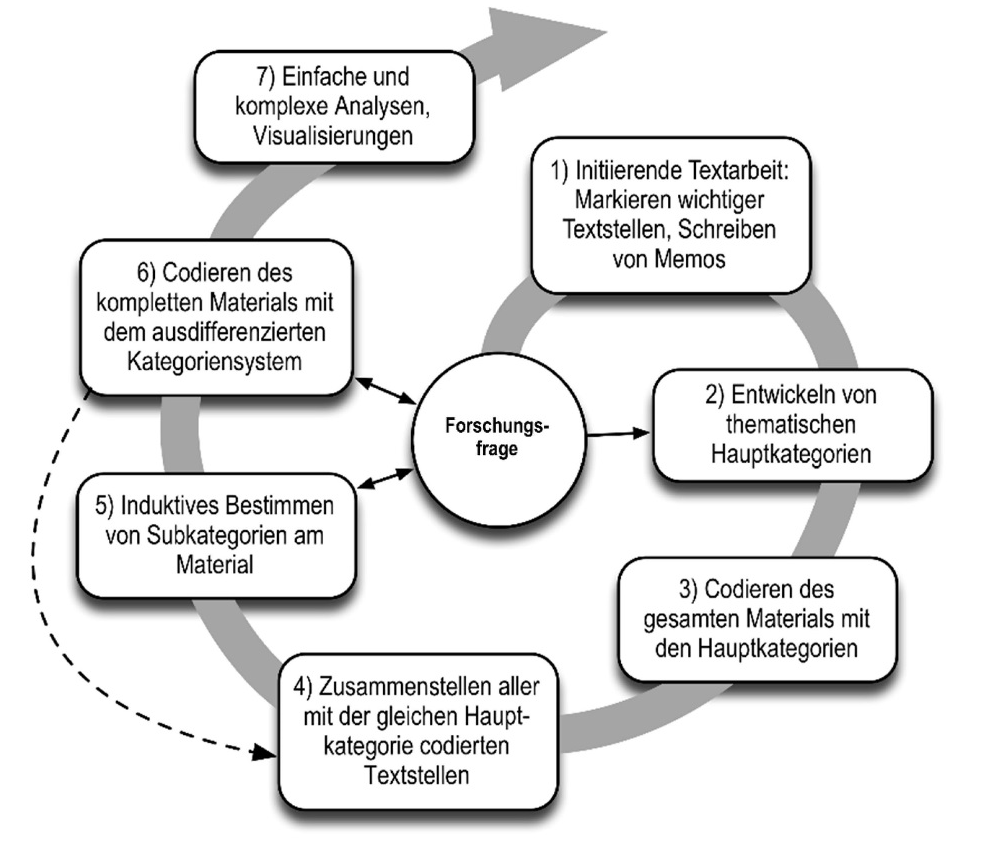
\includegraphics[width=.8\linewidth]{thesis/images/Kuckartz_Ablaufschema-inhaltlich-strukturierenden-Inhaltsanalyse.png}
    \caption[blaufschema einer inhaltlich strukturierenden Inhaltsanalyse nach Kuckartz]{Ablaufschema einer inhaltlich strukturierenden Inhaltsanalyse nach Kuckartz \cite[100]{kuckartz_qualitative_2018}}
    \label{fig:ablaufschema-inhaltlich-strukturierende-inhaltsanalyse}
\end{figure}

\subsection{Thematische Hauptkategorien}
\label{sub-sec:thematische-hauptkategorien}

Anhand der von Kuckartz beschriebenen Herangehensweise stellt der erste Schritt der inhaltlich strukturierenden Analyse die Bildung von thematischen Hauptkategorien dar, die als Kategorien zur Auswertung verwendet werden. Die Themen beziehungsweise Kategorien beziehen sich dabei häufig auf die Forschungsfrage der Arbeit oder finden sich im Leitfaden der durchgeführten Interviews wieder. Die Kategorien können dabei sowohl anhand des vorliegenden Materials als auch im Vorhinein erstellt und im Anschluss zur Klassifizierung angewandt werden. \cite[101\psq]{kuckartz_qualitative_2018}

\medskip

Anhand des Interviewleitfadens, welcher in Anhang \ref{appendix:interview-leitfaden} ab Seite \pageref{appendix:interview-leitfaden} ersichtlich ist, sowie der beiden Einzelinterviews (siehe Anhang \ref{appendix:interview-1} ab Seite \pageref{appendix:interview-1} sowie Anhang \ref{appendix:interview-2} ab Seite \pageref{appendix:interview-2}) und der Gruppendiskussion (siehe Anhang \ref{appendix:gruppendiskussion} ab Seite \pageref{appendix:gruppendiskussion}) können die folgenden Themenschwerpunkte für die anschließende Kategorisierung definiert werden\footnote{Die in den Einzelinterviews und der Gruppendiskussion gestellten Fragen und erhaltenen Antworten enthalten stellenweise Themenbereiche, die nur eine untergeordnete Rolle spielen oder keine Relevanz für die tatsächliche Analyse der Anforderungen für ein neues Ethikantrag-Tool haben. Diese Fragen und auch Antworten werden bei der Findung der Hauptthemen und auch in der darauf aufbauenden qualitativen Inhaltsanalyse außen vor gelassen.}:
\begin{itemize}
    \item Prozess beziehungsweise Ablauf eines Ethikantrages
    \item Feedback, Kritik und Verbesserungsvorschläge
    \item Anforderungen an ein überarbeitetes System oder Tool
\end{itemize}

\subsubsection*{Anmerkungen}
\label{sub-sub-sec:thematische-hauptkategorien-anmerkungen}

Die Anzahl an Hauptthemen fällt relativ gering aus, da der Fokus der geführten Interviews -- mit der Erstellung und Einreichung von Ethikanträgen und dem zugrundeliegenden Prozess -- relativ eng gesteckt ist.

Die Kategorien \textit{Feedback, Kritik und Verbesserungsvorschläge} und \textit{Anforderungen an ein überarbeitetes System oder Tool} ähneln sich zudem auf den ersten Blick dahingehend, dass beide zu einem gewissen Teil sowohl Feedback, Anforderung und Verbesserungsvorschlag als auch Wunsch in einem enthalten. Die beiden Themen sind jedoch spezifisch getrennt worden, da im Zuge der Codierung eine unverbindlich vorgeschlagene Idee beziehungsweise Verbesserung von einem absoluten \enquote{Must Have} oder auch einer eindeutig geforderten Änderung unterschieden werden.

\subsubsection*{Zwischenergebnis der Kategorisierung anhand der Hauptkategorien}
\label{sub-sub-sec:zwischenstand-hauptkategorisisierung}

Abbildung \ref{fig:zwischenstand-hauptkategorisierung} auf Seite \pageref{fig:zwischenstand-hauptkategorisierung} zeigt das Zwischenergebnis der initialen Kategorisierung der zwei Einzelinterviews sowie der Gruppendiskussion. Im jeweiligen Feld lässt sich dabei die Anzahl der Kategorisierungen der entsprechenden Hauptkategorie (im Kontext der \ac{qda}-Software MAXQDA\footnote{MAXQDA (\url{https://www.maxqda.com/de/})} \enquote{Code} beziehungsweise \enquote{Codesystem}) erkennen.

\begin{figure}[ht]
    \centering
    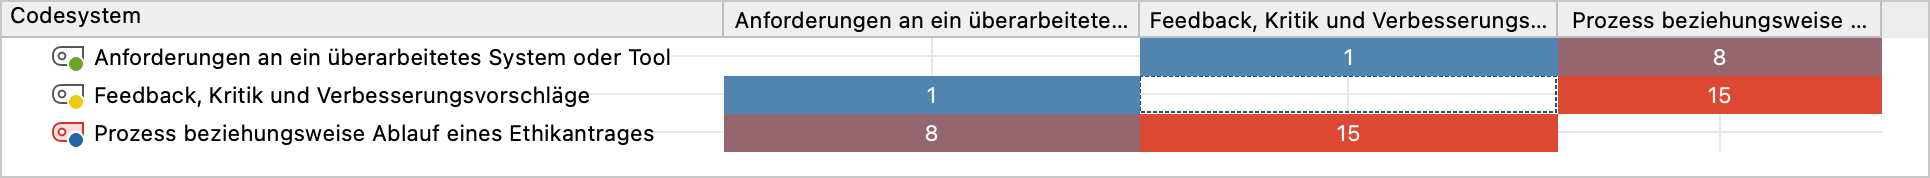
\includegraphics[width=\linewidth]{thesis/images/Luidold_Hauptkategorien-Zwischenergebnis.png}
    \caption[Zwischenergebnis der initialen Kategorisierung anhand der Hauptkategorien]{Zwischenergebnis der initialen Kategorisierung anhand der Hauptkategorien (Quelle: eigene Abbildung)}
    \label{fig:zwischenstand-hauptkategorisierung}
\end{figure}

Bereits nach der initialen Kategorisierung lässt sich grundlegend feststellen, dass beim Thematisieren des \textit{Prozesses beziehungsweise Ablaufes eines Ethikantrages} häufig auch \textit{Feedback, Kritik und Verbesserungsvorschläge} zur Sprache kommen oder \textit{Anforderungen an ein überarbeitetes System oder Tool} gestellt werden.

\subsection{Thematische Subkategorien anhand des Materials}
\label{sub-sec:thematische-subkategorien}

Um ein genaueres Verständnis über die Zusammenhänge gewinnen und Anforderungen ableiten zu können, schlägt Kuckartz als nächsten Schritt vor, Subkategorien auf Basis des Materials zu definieren, welches bereits mit den Hauptkategorien klassifiziert wurde. \cite[106]{kuckartz_qualitative_2018}

Im Zuge der erneuten Durchsicht des Materials und der anschließenden zweiten Codierung der Einzelinterviews und der Gruppendiskussion konnten insgesamt elf Subkategorien ausfindig gemacht und definiert werden. Das in MAXQDA schlussendlich definierte \enquote{Codesystem} kann in Abbildung \ref{fig:angewandtes-codesystem} auf Seite \pageref{fig:angewandtes-codesystem} nachvollzogen werden.

\begin{figure}[ht]
    \centering
    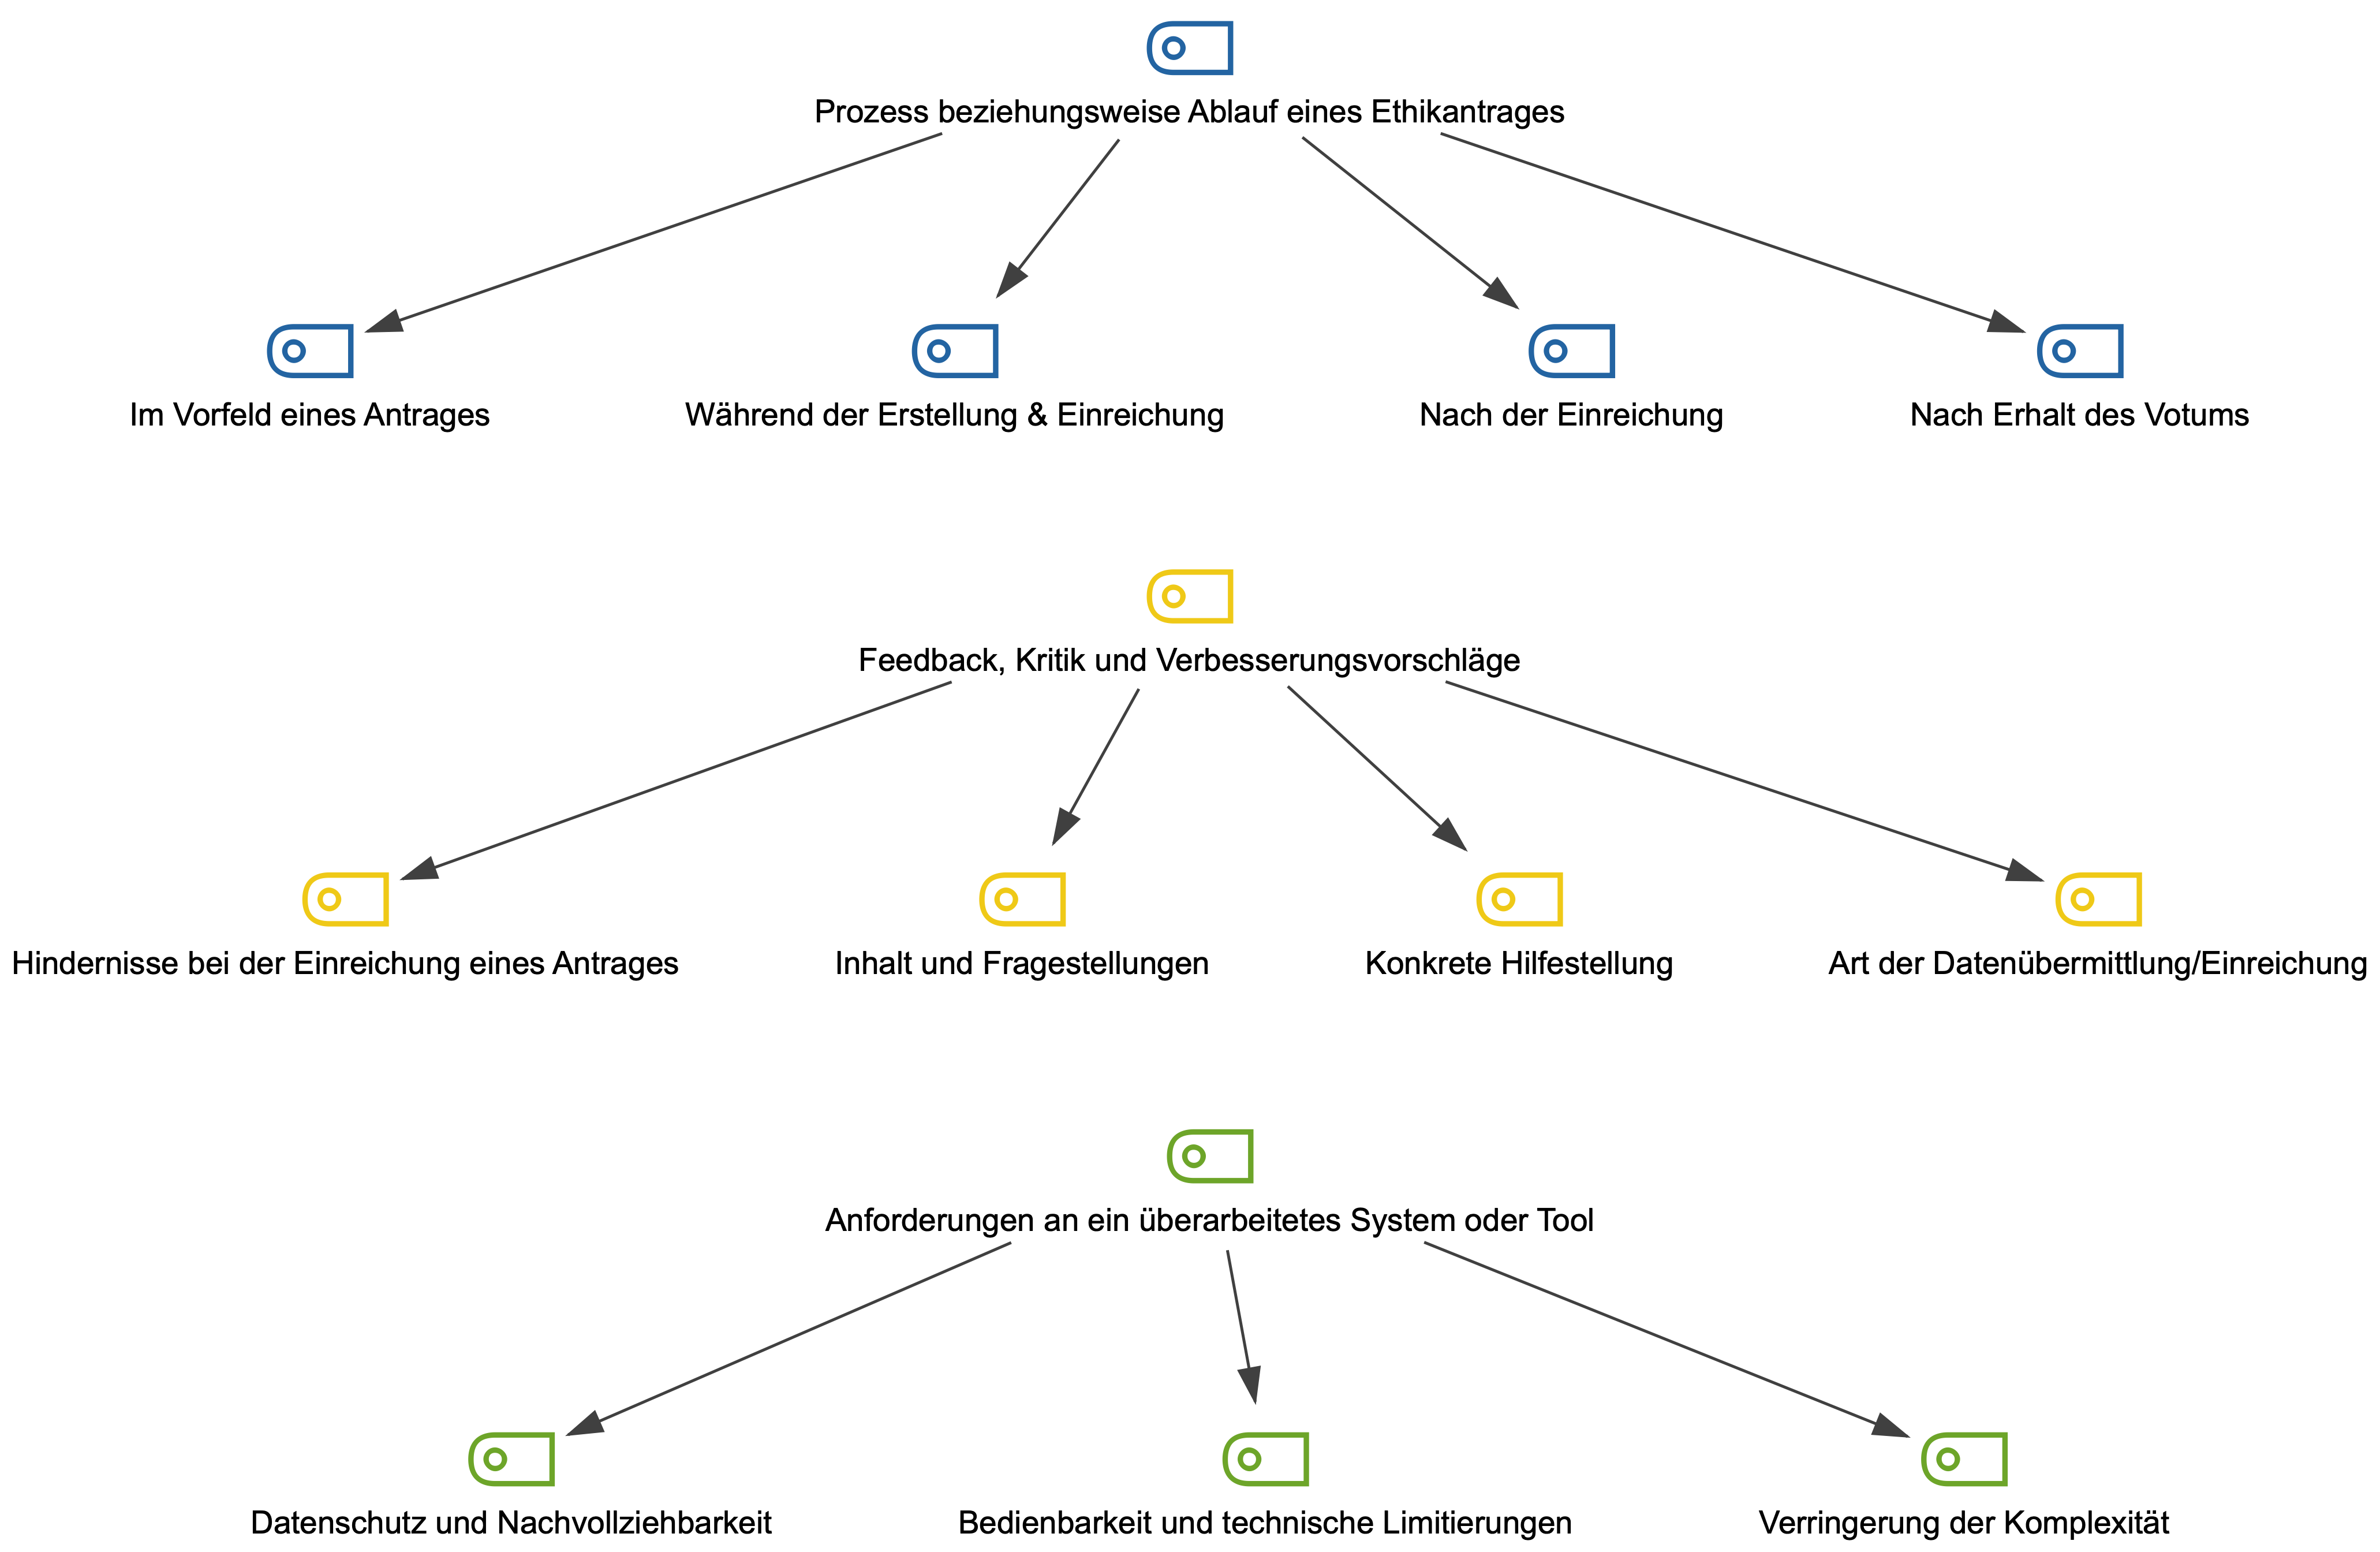
\includegraphics[width=\linewidth]{thesis/images/Luidold_Codesystem.png}
    \caption[Ausgearbeitetes und angewandtes Codesystem zur Codierung der Interviews und Gruppendsikussion]{Ausgearbeitetes und angewandtes Codesystem zur Codierung der Interviews und Gruppendsikussion (Quelle: eigene Abbildung)}
    \label{fig:angewandtes-codesystem}
\end{figure}

\subsection{Ergebnis der Klassifizierung}
\label{sub-sec:ergebnis-klassifizierung}

Das Ergebnis der Klassifizierung wird laut Kuckartz nun eigentlich mittels detaillierter fallbezogener thematischer Zusammenfassung genauer aufgearbeitet und auf Basis dessen analysiert und visualisiert. \cite[111-121]{kuckartz_qualitative_2018} Aufgrund der angesprochenen zeitlichen Einschränkung beschränkt sich die fallbezogene thematische Zusammenfassung auf die in Abschnitt \ref{sec:stärken-schwächen-probleme} ab Seite \pageref{sec:stärken-schwächen-probleme} durchgeführte Analyse der Stärken, Schwächen und Probleme, welche auf den Ergebnissen dieses Kapitels basiert.

\medskip

Eine detailliertere Analyse lässt sich nun Anhand der von MAXQDA bereitgestellten \enquote{Code-Relations-Browser} Funktionalität umsetzen, welche auch schon in Abbildung \ref{fig:zwischenstand-hauptkategorisierung} auf Seite \pageref{fig:zwischenstand-hauptkategorisierung} zum Einsatz gekommen ist. Abbildung \ref{fig:feedback-x-prozess} auf Seite \pageref{fig:feedback-x-prozess} stellt dabei als ersten Schritt den Zusammenhang zwischen dem in den Interviews und der Gruppendiskussion geäußerten Feedback mit den jeweiligen Prozessabschnitten dar.

\begin{figure}[ht]
    \centering
    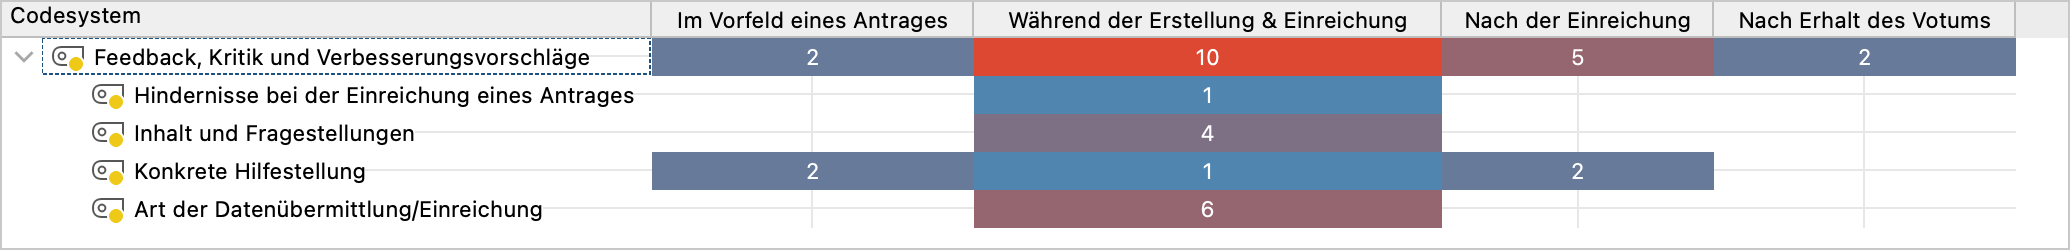
\includegraphics[width=\linewidth]{thesis/images/Luidold_Feedback-Prozess.png}
    \caption[Zusammenhang zwischen genanntem Feedback und den einzelnen Prozessabschnitten]{Zusammenhang zwischen genanntem Feedback und den einzelnen Prozessabschnitten (Quelle: eigene Abbildung)}
    \label{fig:feedback-x-prozess}
\end{figure}

Anhand der Auswertung lässt sich feststellen, dass eingebrachtes Feedback vor allem die Erstellung und Einreichung eines Ethikantrages betrifft, während es im Vorfeld zu einem Antrag und auch nach der Einreichung sowie dem Erhalt des Votums deutlich weniger Anregungen und Probleme gibt. Diese Feststellung deckt sich auch mit der in der in Abschnitt \ref{sec:motivation} sowie Abschnitt \ref{sec:frage-problemstellung} ab Seite \pageref{sec:motivation} beziehungsweise \pageref{sec:frage-problemstellung} dargelegten Motivation und Problemstellung.

\medskip

Neben dem getätigten Feedback konnten in den Interviews und der Gruppendiskussion auch Aussagen klassifiziert werden, die aufgrund der expliziten Nennung nicht nur als Verbesserungsvorschlag oder Wunsch sondern als konkrete Anforderung zu definieren sind. Abbildung \ref{fig:anforderungen-x-prozess} auf Seite \pageref{fig:anforderungen-x-prozess} zeigt die Verteilung der Anforderungen in Bezug auf die einzelnen Prozessschritte. Es ist deutlich erkennbar, dass diese hauptsächlich die Erstellung und Einreichung eines Ethikantrages sowie den Prozess nach der Einreichung durch die Antragsteller:innen betreffen.

\begin{figure}[ht]
    \centering
    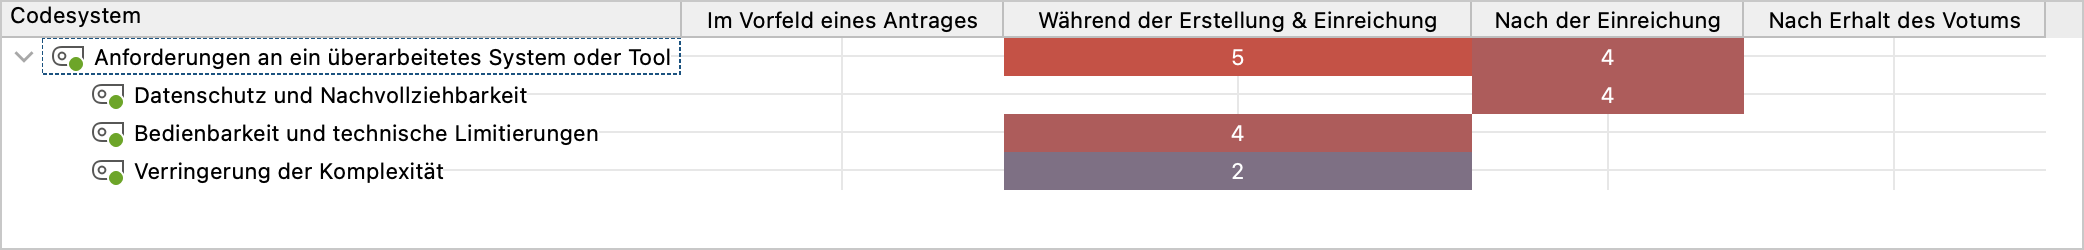
\includegraphics[width=\linewidth]{thesis/images/Luidold_Anforderungen-Prozess.png}
    \caption[Zusammenhang zwischen genannten Anforderungen und den einzelnen Prozessabschnitten]{Zusammenhang zwischen genannten Anforderungen und den einzelnen Prozessabschnitten (Quelle: eigene Abbildung)}
    \label{fig:anforderungen-x-prozess}
\end{figure}

Insgesamt wurden die drei Hauptkategorien und elf Subkategorien 114 Mal zur Codierung von relevanten Passagen und Ausschnitten der Interviews sowie der Gruppendiskussion verwendet. Abbildung \ref{fig:codesystem-anzahl} auf Seite \pageref{fig:codesystem-anzahl} zeigt das Codesystem noch einmal in einer anderen Darstellungsart, wobei neben jedem einzelnen Code die entsprechende Anzahl an Codierungen aufgelistet ist.

Entgegen Kuckartz Empfehlungen (\cite[108]{kuckartz_qualitative_2018}) gibt es mehrere Textpassagen und Antworten, die zwar mit einer Hauptkategorie, nicht aber mit einer Subkategorie (beispielsweise der Kategorie \enquote{Sonstiges}) codiert wurden. Diese Entscheidung wurde bewusst getroffen, um das Codesystem schlank und die Auswertung auf dem sehr überschaubaren Material zielgerichtet zu halten.

\begin{figure}[ht]
    \centering
    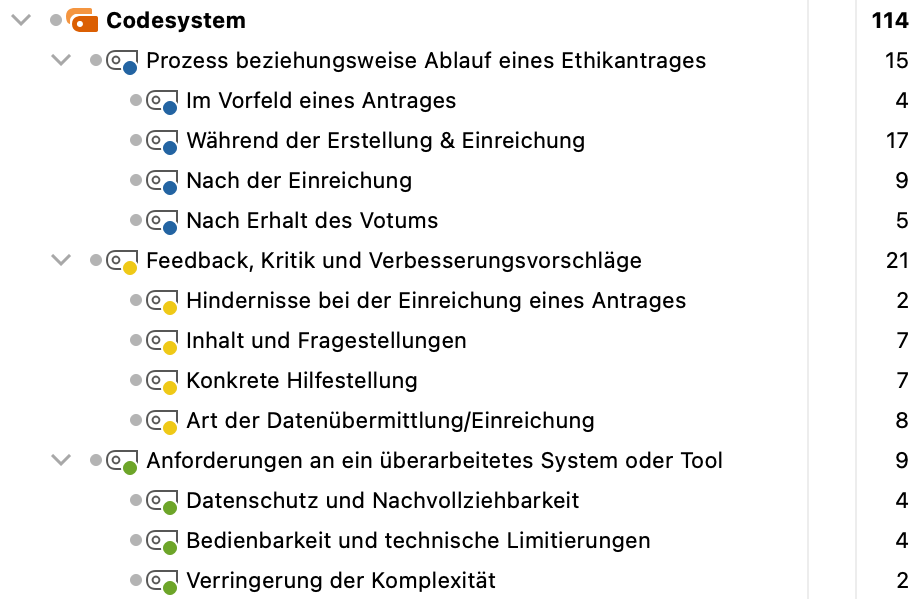
\includegraphics[width=.8\linewidth]{thesis/images/Luidold_Codesystem-Anzahl.png}
    \caption[Angewandtes Codesystem inklusive Anzahl der vorgenommenen Codierungen je Code]{Angewandtes Codesystem inklusive Anzahl der vorgenommenen Codierungen je Code (Quelle: eigene Abbildung)}
    \label{fig:codesystem-anzahl}
\end{figure}

\section{Definition der Anforderungen}
\label{sec:definition-anforderungen}

Anhand der in Abschnitt \ref{sec:qualitative-inhaltsanalyse} ab Seite \pageref{sec:qualitative-inhaltsanalyse} durchgeführten qualitativen Inhaltsanalyse lassen sich im abschließenden Schritt nun die konkreten Anforderungen an ein neues System und gegebenenfalls einen neuen Prozess definieren. Die Anforderungen werden dabei mit codierten Textstellen aus den Interviews und der Gruppendiskussion belegt, wobei inhaltlich doppelte Nennungen zusammengefasst beziehungsweise weggelassen werden. Ebenso werden Textpassagen außen vor gelassen, die zwar codiert wurden, im Rahmen anderer Anforderungen aber bereits abgedeckt werden konnten und starke inhaltliche Ähnlichkeiten aufweisen.

\subsection{Im Vorfeld eines Antrages}
\label{sub-sec:vorfeld-antrag}

Tabelle \ref{tab:anforderungen-vorfeld-antrag} auf Seite \pageref{tab:anforderungen-vorfeld-antrag} zeigt sämtliche Textausschnitte auf, die entweder der Haupt- oder Subkategorie \textit{Feedback, Kritik und Verbesserungsvorschläge} oder \textit{Anforderungen an ein überarbeitetes System oder Tool} zugeordnet sind und im Rahmen der Kategorie \textit{Im Vorfeld eines Antrages} vorkommen.

\begin{table}[ht]
    \centering
    \begin{tabular}{p{.05\linewidth} | p{.2\linewidth} | p{.65\linewidth}}
        \# & \textbf{Interview} & \textbf{Textausschnitt}\\
        \hline
        1 & Einzelinterview \#2 & \textit{Dominic:} In dem Fall für dich ganz klar gewesen oder für euch im Forschungsprojekt, dass da ein Ethikantrag wirklich notwendig ist?\newline \textit{Interviewpartner:in B:} [...] Es ist natürlich immer etwas schwierig, ab wann braucht man sowas, braucht man für einen normalen Usability-Test einen Ethikantrag? Also da sind die Grenzen schon noch etwas schwammig und da wär eine Unterstützung von einem Tool sicher hilfreich das zu entscheiden, ob es überhaupt einen Ethikantrag braucht.
    \end{tabular}
    \caption{Textausschnitte der Interviews und Gruppendiskussion zu Punkten im Vorfeld eines Ethikantrages}
    \label{tab:anforderungen-vorfeld-antrag}
\end{table}

\subsubsection*{Analyse}
\label{sub-sub-sec:analyse-vorfeld-antrag}

\textit{Interviewpartner:in B} äußert eine Aussage (\hyperref[tab:anforderungen-vorfeld-antrag]{\#1}), die als \textit{Konkrete Hilfestellung} codiert ist und darauf hinweist, dass es nicht immer eindeutig ist, wann ein Ethikantrag erforderlich ist. Als konkretes Beispiel wird ein \enquote{Usability-Test} genannt, bei dem Unsicherheit besteht, ob ein entsprechendes Votum der \ac{fek} erforderlich ist oder nicht.

\subsubsection*{Abgeleitete Anforderungen}
\label{sub-sub-sec:abgeleitete-anforderungen-vorfeld-antrag}

Daraus abgeleitet lassen sich folgende Anforderungen definieren:
\begin{enumerate}[label=\textbf{\#\arabic*}]
    \item Das Ethikantrags-Tool soll klarere Richtlinien und auch Hilfestellungen bereitstellen, um die Entscheidung zu unterstützen, ob ein Ethikantrag erforderlich ist.
\end{enumerate}

\subsection{Während der Erstellung \& Einreichung}
\label{sub-sec:während-erstellung-einreichung}

Tabelle \ref{tab:anforderungen-während-erstellung-einreichung} auf Seite \pageref{tab:anforderungen-während-erstellung-einreichung} fasst die Textausschnitte zusammen, die entweder der Haupt- oder Subkategorie \textit{Feedback, Kritik und Verbesserungsvorschläge} oder \textit{Anforderungen an ein überarbeitetes System oder Tool} zugeordnet sind und im Rahmen der Kategorie \textit{Während der Erstellung \& und Einreichung eines Antrages} vorkommen. Wie eingangs erwähnt, werden inhaltliche Überschneidungen und doppelte Nennungen zugunsten der Übersicht auf einzelne, gleichwertige Textausschnitte heruntergebrochen.

\begin{table}[ht!]
    \centering
    \begin{tabular}{p{.05\linewidth} | p{.2\linewidth} | p{.65\linewidth}}
        \# & \textbf{Interview} & \textbf{Textausschnitt}\\
        \hline
        2 & Einzelinterview \#1 & \textit{Interviewpartner:in A:} [...] Vielleicht wäre das eine Vereinfachung, wenn man das alles in digitaler Form einreichen kann, dass das nicht per E-Mail hin und her geschickt werden muss. [...] \\
        \hline
        3 & Einzelinterview \#2 & \textit{Interviewpartner:in B:} [...] Also es sind auch einige Dinge die einem so vorkommen zumindest, dass sie doppelt ausgefüllt werden müssen, je nachdem, ob es ein Produkt wird oder ob es nur eine Forschung ist, dass man da unterschiedliche Blätter ausfüllen muss. \\
        \hline
        4 & Einzelinterview \#2 & \textit{Interviewpartner:in B:} [...]  Das wäre vielleicht auch so eine Idee, dass man da mittracken kann, wer was hinzu geschrieben hat und von wem welcher Input gekommen ist. \\
        \hline
        5 & Gruppen-diskussion & \textit{Dominic:} Wenn ich da eingreifen darf, was wären denn für euch Formatierungsmöglichkeiten? [...]\newline
        \textit{Interviewpartner:in E:} Bulletpoints, das wäre gut. Strukturierungselemente in irgend einer Form.\newline\
        \textit{Interviewpartner:in C:} Nichts fett. Keine Bilder.\newline
        \textit{Interviewpartner:in F:} Ich bin auch eher der hermeneutische Typ. Ich hätte null Möglichkeiten vorgesehen, aber Bulletpoints sind Okay. Aber sonsten nada. \\
        \hline
        6 & Gruppen-diskussion & \textit{Interviewpartner:in D:} [...] Nicht mühsam sein soll es, dieses Formular auszufüllen. Da soll es wirklich nicht daran scheitern, dass man nicht irgendwo in einem anderen Dokument vorschreiben und es dann hineinkopieren kann. Das muss eigentlich klappen. Und auch, dass man innerhalb des Dokumentes ordentlich zitieren kann [...]. [...] das Ausfüllen des Formulares [...] soll eben einfach von statten gehen. \\
    \end{tabular}
    \caption{Textausschnitte der Interviews und Gruppendiskussion zu Punkten während der Erstellung \& Einreichung eines Ethikantrages}
    \label{tab:anforderungen-während-erstellung-einreichung}
\end{table}

\subsubsection*{Analyse}
\label{sub-sub-sec:analyse-während-erstellung-einreichung}

\textit{Interviewpartner:in A} erwähnt während des Interviews (\hyperref[tab:anforderungen-während-erstellung-einreichung]{\#2}) zur \textit{Art der Datenübermittlung}, dass eine Einreichung der Unterlagen sowie dem Ethikantrag selbst per E-Mail nicht optimal ist. Ähnliches wurde auch von den Mitgliedern der \ac{fek} rückgemeldet.

\medskip

\textit{Interviewpartner:in B} nennt zum Thema \textit{Inhalt und Fragestellung} (\hyperref[tab:anforderungen-während-erstellung-einreichung]{\#3}), dass im Antragsformular gewisse Themenaspekte mehrfach angegeben werden müssen, abhängig davon, was für ein Forschungsprojekt umgesetzt wird. Vereinzelt haben Mitglieder der \ac{fek} dazu ähnliches Feedback geäußert.

\medskip

\textit{Interviewpartner:in B} schlägt als \textit{konkrete Hilfestellung} vor (\hyperref[tab:anforderungen-während-erstellung-einreichung]{\#4}), dass protokolliert werden könnte, wer welche Änderungen an einem Antrag vornimmt, sofern dieser von mehren Personen innerhalb des Forschungsprojektes bearbeitet wird.

\medskip

\textit{Interviewpartner:innen C, E und F} stellen während der Diskussion (\hyperref[tab:anforderungen-während-erstellung-einreichung]{\#5}) die Anforderung an die \textit{Bedienbarkeit und technische Limitierung}, dass Formatierungsmöglichkeiten in einem neuen System ebenfalls rein auf Text und Zeichen beschränkt werden sollen. Lediglich Bulletpoints sollen als Strukturelemente ermöglicht werden.

\medskip

\textit{Interviewpartner:in D} stellt die Anforderung (\hyperref[tab:anforderungen-während-erstellung-einreichung]{\#6 }) sowohl an die \textit{Verringerung der Komplexität} als auch die \textit{Bedienbarkeit und technischen Limitierungen}, dass das Formular einfach auszufüllen sein muss und dass sowohl grundlegende Funktionen wie das Kopieren und Einfügen von Text als auch Literaturverwaltungsprogramme unterstützt werden sollen.

\subsubsection*{Abgeleitete Anforderungen}
\label{sub-sub-sec:abgeleitete-anforderungen-während-erstellung-einreichung}

Daraus abgeleitet lassen sich folgende Anforderungen definieren:
\begin{enumerate}[label=\textbf{\#\arabic*}]
    \setcounter{enumi}{1}
    \item Die Übermittlung eines Ethikantrages sowie zugehöriger Unterlagen soll nicht mehr mittels E-Mail erfolgen.
    \item Der Ethikantrag soll berücksichtigen, dass es unterschiedliche Typen von Forschungsvorhaben gibt und die Fragen darauf abstimmen, um doppelte Fragestellungen dazu vermeiden zu können.
    \item Das System soll protokollieren, wer welche Änderungen an einem (noch nicht eingereichten) Ethikantrag vorgenommen hat.
    \item Das System soll ausschließlich Zeichen und keine weiteren Formatierungen mit Außnahme von Bulletpoints zulassen.
    \item Das System soll weiterführende Funktionen wie beispielsweise die Integration von Literaturverwaltungsprogrammen unterstützen.
\end{enumerate}

\subsection{Nach der Einreichung}
\label{sub-sec:nach-einreichung}

Tabelle \ref{tab:anforderungen-nach-einreichung} auf Seite \pageref{tab:anforderungen-nach-einreichung} fasst die Textausschnitte zusammen, die entweder der Haupt- oder Subkategorie \textit{Feedback, Kritik und Verbesserungsvorschläge} oder \textit{Anforderungen an ein überarbeitetes System oder Tool} zugeordnet sind und im Rahmen der Kategorie \textit{Nach der Einreichung} vorkommen. Wie eingangs erwähnt, werden inhaltliche Überschneidungen und doppelte Nennungen zugunsten der Übersicht auf einzelne, gleichwertige Textausschnitte heruntergebrochen.

\begin{table}[ht!]
    \centering
    \begin{tabular}{p{.05\linewidth} | p{.2\linewidth} | p{.65\linewidth}}
        \# & \textbf{Interview} & \textbf{Textausschnitt}\\
        \hline
        7 & Einzelinterview \#2 & \textit{Interviewpartner:in B:} [...] Da wäre es interessant, wenn es so eine Prozessansicht geben würde, wo man sieht, wo steckt der Antrag gerade, er ist jetzt in Begutachtung, die Kommission muss zusammentreffen und das nächste Treffen findet dann und dann statt. \\
        \hline
        8 & Gruppen-diskussion & \textit{Interviewpartner:in E:} [...] Zur Entlastung des:der Vorsitzenden würde ich aktuell sagen [...] automatisierte Eingangsbestätigungen, vielleicht eine automatisierte Mail wenn es um gewisse Prozesse, administrative Informationsaspekte geht, die automatisierbar sind. [...]\newline
        \textit{Interviewpartner:in D:} Also gerade der formale Check könnte sich durchaus automatisieren lassen. Das wäre schon eine E-Mail, zwei E-Mails weniger. \\
        \hline
        9 & Gruppen-diskussion & \textit{Interviewpartner:in F:} [...] Wir müssen, wenn wir zusammen kommen und eine Entscheidung über einen Antrag stellen, ein gemeinsames verbindliches Dokument haben, auf Basis dessen wir entscheiden. Das heißt, wir müssen auch die Möglichkeit haben, die Meta-Daten aus so einem Dokument, egal wie lange aber Minimum die üblichen drei Jahre, oder sieben Jahre, das kann man definieren, die müssen gesichert irgendwo gespeichert sein. [...]
    \end{tabular}
    \caption{Textausschnitte der Interviews und Gruppendiskussion zu Punkten nach der Einreichung eines Ethikantrages}
    \label{tab:anforderungen-nach-einreichung}
\end{table}

\subsubsection*{Analyse}
\label{sub-sub-sec:analyse-nach-einreichung}

\textit{Interviewpartner:in B} schlägt als \textit{konkrete Hilfestellung} vor (\hyperref[tab:anforderungen-nach-einreichung]{\#7}), dass nach der Einreichung eines Antrages genauere Informationen darüber bereitgestellt werden könnten, in welchem Stadium sich der eingereichte Antrag gerade befindet.

\medskip

\textit{Interviewpartner:in E und F} schlagen als \textit{konkrete Hilfestellung} vor (\hyperref[tab:anforderungen-nach-einreichung]{\#8}), dass zur Entlastung des Vorsitzes der \ac{fek} genereische E-Mails automatisiert versendet und auch ein initialer formaler Check automatisch vorgenommen werden könnte.

\medskip

\textit{Interviewpartner:in D} stellt eine Anforderung (\hyperref[tab:anforderungen-nach-einreichung]{\#9}) an den \textit{Datenschutz und die Nachvollziehbarkeit}, dass eingereichte Anträge für einen bestimmten Zeitraum gespeichert werden müssen und dass die enthaltenen (Meta-)Informationen während dieser Zeit zugänglich sein sollen.

\subsubsection*{Abgeleitete Anforderungen}
\label{sub-sub-sec:abgeleitete-anforderungen-nach-einreichung}

Daraus abgeleitet lassen sich folgende Anforderungen definieren:
\begin{enumerate}[label=\textbf{\#\arabic*}]
    \setcounter{enumi}{6}
    \item Das System soll eine Möglichkeit bieten, nachvollziehen zu können, in welchem Stadium sich ein eingereichter Ethikantrag befindet.
    \item Das System soll automatisierbare Arbeitsschritte wie den E-Mail-Versand und den formalen Check von Unterlagen selbstständig übernehmen.
    \item Das System soll eine nachvollziehbare, eindeutige und sichere Speicherung der Daten für einen beliebig langen Zeitraum ermöglichen.
\end{enumerate}

\subsection{Nach Erhalt des Votums}
\label{sub-sec:nach-erhalt-votum}

Es wurden zwar mehrere Codierungen mittels dem Code \textit{Nach Erhalt des Votums} vorgenommen, es lassen sich jedoch daraus keine neuen Schlüsse ziehen, die nicht schon durch die vorherigen Definitionen etwaiger Anforderungen abgedeckt werden konnten.

\section{Priorisierung der Anforderungen}
\label{sec:priorisierung-anforderungen}

Der Rahmen dieser Masterarbeit erstreckt sich, wie in Abschnitt \ref{sec:zielsetzung} ab Seite \pageref{sec:zielsetzung} bereits erläutert, auf die Umsetzung eines \ac{poc} anhand eines Prototyps. Die in Abschnitt \ref{sec:definition-anforderungen} ab Seite \pageref{sec:definition-anforderungen} definierten neun Anforderungen können und sollen im Zuge dessen nicht vollständig umgesetzt werden, weshalb eine entsprechende Priorisierung vorgenommen werden muss.

\medskip

Der Fokus des angestrebten \ac{poc} beruht dabei vor allem auf der Erstellung und Einreichung eines Ethikantrages, während die weiterführende Behandlung eines Antrages durch die \ac{fek} nicht zu den unmittelbaren Zielen gehört. Tabelle \ref{tab:priorisierung-anforderungen} auf Seite \pageref{tab:priorisierung-anforderungen} berücksichtigt diesen Umstand und nimmt die Priorisierung anhand des in \cite{chai_what_2020} definierten Eisenhower-Prinzips vor.

\begin{table}[ht!]
    \centering
    \begin{tabular}{p{.15\linewidth} | p{.35\linewidth} | p{.35\linewidth}}
        & \textbf{Dringend} & \textbf{Nicht Dringend} \\
        \hline
        \textbf{Wichtig} & \hyperref[sub-sub-sec:abgeleitete-anforderungen-vorfeld-antrag]{\#1}, \hyperref[sub-sub-sec:abgeleitete-anforderungen-während-erstellung-einreichung]{\#2}, \hyperref[sub-sub-sec:abgeleitete-anforderungen-während-erstellung-einreichung]{\#3}, \hyperref[sub-sub-sec:abgeleitete-anforderungen-während-erstellung-einreichung]{\#5},  \hyperref[sub-sub-sec:abgeleitete-anforderungen-nach-einreichung]{\#8} & \hyperref[sub-sub-sec:abgeleitete-anforderungen-während-erstellung-einreichung]{\#4}, \hyperref[sub-sub-sec:abgeleitete-anforderungen-während-erstellung-einreichung]{\#6}, \hyperref[sub-sub-sec:abgeleitete-anforderungen-nach-einreichung]{\#7}, \hyperref[sub-sub-sec:abgeleitete-anforderungen-nach-einreichung]{\#9} \\
        \hline
        \textbf{Nicht Wichtig} & / & /
    \end{tabular}
    \caption{Priorisierung der definierten Anforderungen nach dem Eisenhower-Prinzip}
    \label{tab:priorisierung-anforderungen}
\end{table}

Das zur Priorisierung angewandte Eisenhower-Prinzip basiert darauf, dass Frage- beziehungsweise Problemstellungen oder geplante Aufgaben in vier Quadranten aufgeteilt werden können, die durch die Einteilung in die Spalten \textit{Dringend} und \textit{Nicht Dringend} sowie die Zeilen \textit{Wichtig} und \textit{Nicht Wichtig} zustande kommen. Die Quadranten entsprechen dabei gleichzeitig auch der Priorisierung, wobei \textit{Dringend und Wichtig} die höchste und \textit{Nicht Dringend und Nicht Wichtig} die niedrigste Priorisierung darstellt. \cite{chai_what_2020}

Alle definierten Anforderungen finden sich in den ersten beiden Quadranten wieder. Dies lässt sich grundlegend damit erklären, dass die von den Interviewpartner:innen angesprochenen Themenpunkte eine wichtige Rolle bei einer Neuentwicklung des Systems und gegebenenfalls auch des Prozesses spielen, während weniger wichtige Themen kaum oder gar nicht angesprochen wurden.

\medskip

Im Zusammenhang mit der Priorisierung kann Anforderung \hyperref[sub-sub-sec:abgeleitete-anforderungen-während-erstellung-einreichung]{\#3} genauer betrachtet und möglicherweise eine Zeile nach unten verschoben werden. Die inhaltliche Ausarbeitung des Ethikantrags liegt letztendlich bei der \ac{fek} der \ac{fhv} und kann während dieser Umsetzung nur begrenzt angepasst werden. Dennoch wird diese Anforderung in derselben Priorisierungsstufe beibehalten, da sie technische Implikationen für zukünftige Änderungen mit sich bringt.

\chapter{Ausarbeitung \& Umsetzung des Prototyps}
\label{chap:ausarbeitung-umsetzung-prototyp}

Anhand der Analyse des Nutzerkontextes und der Definition konkreter Anforderungen (siehe dazu Kapitel \ref{chap:user-centered-design} ab Seite \pageref{chap:user-centered-design} sowie konkret die in Abschnitt \ref{sec:ucd-verknüpfung-arbeit} ab Seite \pageref{sec:ucd-verknüpfung-arbeit} definierten Verknüpfungen mit den Kapiteln dieser Arbeit) ist es im nächsten Schritt nun möglich, mit der Umsetzung eines ersten Konzeptes sowie des darauf aufbauenden, initialen Prototyps und \aclp{poc} zu beginnen.

Das folgende Kapitel beschäftigt sich im Zuge dessen daher sowohl mit dem Aspekt des \aclp{ui} sowie der \ac{ux}, der verwendeten Design-Elemente und der zur Verfügung stehenden Funktionalitäten als auch mit der zugrundeliegenden technischen Umsetzung. Dabei wird jeweils begründet, warum und weshalb welche Ansätze und Herangehensweisen gewählt wurden und welche möglichen (langfristigen) Implikationen diese haben.

\section{Wahl der technischen Basis}
\label{sec:ausarbeitung-wahl-technische-basis}

Um das Konzept beziehungsweise den angedachten Prototyp umsetzen zu können, muss grundlegend eine Entscheidung getroffen werden, welche technische Basis für die Entwicklung und Umsetzung der in Abschnitt \ref{sec:definition-anforderungen} ab Seite \pageref{sec:definition-anforderungen} definierten Anforderungen verwendet werden soll. Die in Abschnitt \ref{chap:analyse-anderer-prozesse} ab Seite \pageref{chap:analyse-anderer-prozesse} durchgeführte Analyse von anderen Prozessen und Systemen dient dabei als Grundlage, um eine begründete weiterführende Entscheidung treffen zu können. Die schlussendliche Auswahl beschränkt sich dabei jedoch nicht ausschließlich auf die analysierten Systeme, sondern setzt sich kritisch mit den jeweiligen Gegebenheiten auseinander.

\subsubsection*{Systeme mit Fokus auf Ethikanträgen}
\label{sub-sub-sec:technische-basis-fokus-ethikanträge}

Vor allem das \acl{ecs} der Medizinischen Universitäten Wien, Innsbruck und weiterer Einrichtungen sticht als System mit direkter Verbindung zum Antragswesen von Ethikanträgen als mögliche Basis hervor. Der in Abschnitt \ref{sub-sec:ecs} ab Seite \pageref{sub-sec:ecs} angesprochene Funktionsumfang und Detaillierungsgrad des Systems stellt auf den ersten Blick eine geeignte Ausgangsposition dar, um die entsprechenden Anpassungen für die definierten Anforderungen vornehmen zu können.

Bei genauerer Betrachtung der technischen Gegebenheiten (welche im genannten Abschnitt auch in Bezug auf die \ac{dx} nur teilweise aufgearbeitet wurden) differenziert sich dieses Bild jedoch:
\begin{itemize}
    \item Das \ac{ecs} setzt als Basis des Applikations-Stack auf ein Ubuntu-Image der Version \texttt{16.04 LTS}. Diese Version wurde erstmals im Jahr 2016 veröffentlicht und enthält laut dem Entwickler Canonical bis Anfang 2026 Sicherheitsupdates im Rahmen des sogenannten \textit{Extended Security Maintenance} Programms. Das letzte verfügbare Update, Version \texttt{16.04.7}, wurde jedoch im August 2020 veröffentlicht. \cite{medizinische_universitat_wien_ecs-handbook_development-2021, canonical_ltd_ubuntu_2023, canonical_ltd_ubuntu_2023-1}
    \item Das \ac{ecs} ist auf zwei Git-Projekte aufgeteilt, die insgesamt über 8.000 Commits in den Repositories aufweisen, welche die Hauptapplikation mit über 196.000 Zeilen Code\footnote{196.780 Zeilen Code; ermittelt anhand von \cite{ethics_commission_system_organization_ecs_2021} und dem Befehl \texttt{git ls-files | xargs wc -l}} beinhalten. \cite{medizinische_universitat_wien_development_2021, ethics_commission_system_organization_ecs_2021, ethics_commission_system_organization_ecs-appliance_2021}
    \item Das \ac{ecs} ist auf eine Nutzung von zwanzig bis hin zu mehreren Hundert Anträgen pro Monat ausgelegt. Der benötigte Speicherplatz bei zwanzig Anträgen pro Monat wird pro zehn Jahre auf zirka 92 GB geschätzt, während die Entwicklungs-Instanz bereits mindestens 10 GB Speicherplatz benötigt. \cite{medizinische_universitat_wien_ecs-handbook_requirements-2021, ethics_commission_system_organization_ecs_2021}
\end{itemize}

Die angesprochenen Punkte stellen an sich, sowohl individuell als auch ganzheitlich betrachtet, keine Hürde dar. Auch unter Berücksichtigung der technischen Analyse in Abschnitt \ref{sub-sec:ecs} ab Seite \pageref{sub-sec:ecs} wird deutlich, dass das \acl{ecs} eine ausgereifte und umfangreiche Software"=Lösung für das Erstellen und Bearbeiten von Ethikanträgen darstellt. Mit der zeitlichen Einschränkung und dem Hintergrund dieser Masterarbeit, eine Software"=Lösung in Form eines Prototyps beziehungsweise eines \ac{poc} zu entwickeln, ändert sich die Ausgangslage jedoch.

Zum Einen ist davon auszugehen, dass eine Aktualisierung des zugrundeliegenden Betriebssystems auf den aktuellsten Stand (laut \cite{canonical_ltd_ubuntu_2023-1} Version \texttt{22.04 LTS} mit initialer Veröffentlichung im April 2022) mit erheblichem Aufwand verbunden ist, um aktuelle Sicherheitsupdates und Funktionalitäten nutzen zu können. Ebenso steigt die Wahrscheinlichkeit, dass die damit einhergehende Aktualisierung der Abhängigkeiten der Applikation zu Komplikationen führen wird. Zusätzlich dazu würde die erforderliche Einarbeitung in das Projekt, um die notwendigen Anpassungen anhand der Anforderungen vornehmen, nicht benötigte Funktionalitäten evaluieren und entfernen sowie neue Möglichkeiten hinzufügen zu können, den Umfang dieser Masterarbeit deutlich überschreiten. Auch im Sinne des Speicherplatzbedarfs stellen die Anforderungen an die Entwicklungsumgebung ein Hindernis dar, um den Prototyp entwickeln und auch testen beziehungsweise evaluieren zu können.

Als abschließende Schlussfolgerung der genannten Punkte kann das \ac{ecs} daher nicht als Basis für die Umsetzung der angedachten Funktionen herangezogen werden.

\subsubsection*{Systeme ohne konkreten Bezug}
\label{sub-sub-sec:technische-basis-systeme-ohne-bezug}

Neben den Systemen mit konkreten Bezug, wovon lediglich das \ac{ecs} als quelloffene Software"=Lösung als mögliche Basis zur Verfügung steht, behandelt Abschnitt \ref{sec:systeme-ohne-bezug} ab Seite \pageref{sec:systeme-ohne-bezug} mehrere Systeme, die eine Umsetzung von Formularen und einem damit verbundenen Antragswesen grundlegend ermöglichen. Bei genauerer Betrachtung und der Einbeziehung der definierten Anforderungen können jedoch auch diese Systeme für die Umsetzung ausgeschlossen werden:
\begin{itemize}
    \item WordPress ist als \ac{cms} primär darauf ausgelegt, benutzerdefinierte Inhalte wie beispielsweise Blog-Artikel oder statische Seiten darzustellen. Wie die Analyse zeigt, werden Plugins und Erweiterungen von Drittanbietern benötigt, um grundlegende Formular-Funktionalitäten bieten zu können. Gerade in Bezug auf die Komplexität der Anforderungen ist nicht ausreichend gewährleistet, dass die zur Verfügung stehenden Erweiterungen diese auch jederzeit erfüllen können, während die Anpassung und Weiterentwicklung von proprietären Erweiterungen eng mit der Unterstützung des jeweiligen Anbieters verknüpft ist, die ebenfalls nicht garantiert werden kann.
    \item Die analysierten Online Formular-Tools von Microsoft und Google können ebenso zwar theoretisch die grundlegenden Anforderungen an die Erstellung eines Online-Formulars erfüllen. Wie in der ursprünglichen Analyse bereits genannt, stellen diese Tools im weiteren Verlauf jedoch keine adäquaten Mittel zur Verfügung, um die eingelangten Daten von Antragsteller:innen in einem einheitlichen System weiter zu verarbeiten, während unabhängig davon Fragen und Unklarheiten zum Datenschutz bestehen.
\end{itemize}

\subsubsection*{Eigenentwicklung als technische Basis}
\label{sub-sub-sec:technische-basis-eigenentwicklung}

Da sich die in Kapitel \ref{chap:analyse-anderer-prozesse} ab Seite \pageref{chap:analyse-anderer-prozesse} analysierten externen Prozesse und Systeme nur bedingt für die Umsetzung eines Konzeptes und Prototyps dieser Arbeit eignen, eine Umsetzung im Rahmen des \acl{ucd} Prozesses jedoch eine essenzielle Rolle spielt, fällt die Entscheidung in Folge dessen auf ein eigens umgesetztes System beziehungsweise eine Eigenentwicklung.

\medskip

Die Wahl des Technologie-Stacks -- sprich der ausgewählten Technologien und Sprachen -- fällt dabei auf das auf JavaScript/TypeScrit aufbauende \ac{spa} Webframework \textit{Angular}\footnote{Angular: \url{https://angular.io/}} für die Umsetzung des \aclp{ui}, während das auf PHP basierende Framework \textit{Symfony}\footnote{Symfony: \url{https://symfony.com/}} für die Domänenlogik sowie die Persistierung und Bereitstellung der Daten zum Einsatz kommt.

Die Frameworks und Technologien wurden zum einen aufgrund bestehender Vorkenntnisse gewählt, zum anderen jedoch vor allem mit dem Hintergedanken, dass damit sowohl das \ac{ui} als auch die \enquote{im Hintergrund} agierende Logik jederzeit unabhängig voneinander ausgetauscht werden können, sollte dies notwendig sein. Genauere technische Erläuterungen und die Erhebung langfristiger Implikationen dieser Entscheidung finden sich in Abschnitt \ref{sec:ausarbeitung-technische-umsetzung} ab Seite \pageref{sec:ausarbeitung-technische-umsetzung} wieder.

\section{Erläuterung des Konzeptes}
\label{sec:erläuterung-konzept}

Für die Ausarbeitung des initialen Konzeptes sowie Prototyps wurden die in Kapitel \ref{chap:analyse-anderer-prozesse} ab Seite \pageref{chap:analyse-anderer-prozesse} erarbeiteten Schlussfolgerungen sowie die in Kapitel \ref{chap:anforderung-neues-system} ab Seite \pageref{chap:anforderung-neues-system} definierten Anforderungen herangezogen. Das daraus resultierende Ergebnis der ersten Umsetzung ist das Konzept der \textit{EthicsVision} Plattform. Diese Plattform ermöglicht Antragssteller:innen als ersten Schritt die Erstellung, Bearbeitung, Einreichung und Anzeige von Ethikanträgen für die \acl{fek} der \acl{fhv} in einer Webapplikation, die über jeden Webbrowser online abrufbar ist. Abbildung \ref{fig:ethics-vision-übersicht} auf Seite \pageref{fig:ethics-vision-übersicht} zeigt die Übersichtsseite der entwickelten Plattform, auf der einige der genannten Funktionen zur Verfügung stehen.

\begin{figure}[ht]
    \centering
    \includegraphics[width=\linewidth]{thesis/images/Luidold_EthicsVision-Übersicht.png}
    \caption{Seite \enquote{Übersicht} der EthicsVision Plattform}
    \label{fig:ethics-vision-übersicht}
\end{figure}

Die Umsetzung als online abrufbare Webapplikation wurde aus mehreren Gründen gewählt: Sowohl die Einreichplattform der FH Campus Wien als auch das \acl{ecs} wurden in ähnlicher Form als Webapplikationen entwickelt und das System der \ac{ieb} soll ebenfalls als Webapplikation umgesetzt werden, was somit dem Stand der Technik entspricht. Darüber hinaus ermöglicht der Fokus auf Webapplikationen die Anwendung weit verbreiteter Technologien, die zum einen die Nutzung auf unterschiedlichen Endgeräten (beispielsweise einem PC, Laptop oder auch Tablet) ermöglichen und zum anderen die Funktionalitäten unabhängig vom jeweiligen Betriebssystem anbieten.

\subsection{Umgesetzte Funktionalitäten}
\label{sub-sec:umgesetzte-funtionalitäten}

Bevor die technische Umsetzung im Detail erläutert wird, werden im folgenden Abschnitt die umgesetzten Funktionalitäten anhand der in Abschnitt \ref{sec:priorisierung-anforderungen} ab Seite \pageref{sec:priorisierung-anforderungen} priorisierten Anforderungen dargelegt und im Zuge dessen in Bezug gestellt. Die entwickelten Lösungen decken dabei nicht immer die gesamte Anforderung ab, was im Zuge \colorbox{yellow}{TODO} der Evaluation des Prototyps in Kapitel \ref{chap:evaluation-prototyp} ab Seite \pageref{chap:evaluation-prototyp} stellenweise noch einmal aufgegriffen wird.

\subsubsection*{Anforderungen \#1 \& \#3}
\label{sub-sub-sec:umgesetzte-funktionalitäten-anforderung-1-3}

\underline{Ausgangslage:} \textit{Anforderung \hyperref[sub-sub-sec:abgeleitete-anforderungen-vorfeld-antrag]{\#1}} gibt vor, dass klare Richtlinien und Hilfestellungen bereitgestellt werden sollen, um die Entscheidung für beziehungsweise gegen einen Ethikantrag zu unterstützen. \textit{Anforderung \hyperref[sub-sub-sec:abgeleitete-anforderungen-während-erstellung-einreichung]{\#3}} gibt vor, dass die unterschiedlichen Typen von Forschungsvorhaben beachtet und Fragen darauf abgestimmt werden sollen.

\medskip

\noindent\underline{Ausgearbeitete Funktionalität:} Die beiden Anforderungen wurden in der EthicsVision Plattform in einer gemeinsamen Software"=Lösung kombiniert. Zu Beginn jeder Antragstellung werden Antragsteller:innen Informationen zum Ethikantrag sowie Verlinkungen zu weiterführendem Informations"=Material der \ac{fek} angeboten, wie in Abbildung \ref{} auf Seite \pageref{} ersichtlich ist. Diese Informationen werden dabei unabhängig von früheren Eingaben dargestellt und sollen erste Anhaltspunkte liefern, ob die Erstellung eines Ethikantrages für das jeweilige Forschungsprojekt notwendig ist.

Wie in Abbildung \ref{fig:ethics-vision-formular-assistent-finanzierung} auf Seite \pageref{fig:ethics-vision-formular-assistent-finanzierung} zu erkennen ist, werden Antragssteller:innen im nächsten Schritt bei der Erstellung eines neuen Ethikantrages unterstützt, diesen den Gegebenheiten des jeweiligen Forschungsvorhabens beziehungsweise -projektes anzupassen. Neben der Finanzierungsgrundlage wird sowohl das Studiendesign als auch die Umsetzung eines Prototyps abgefragt.\footnote{Diese drei Bereiche wurden anhand des bestehenden Antragsformulars gezielt gewählt, da die \ac{fek} abhängig vom Typ des Forschungsvorhabens spezifische Informationen zu den Rahmenbedingungen benötigt sowie unterschiedliche inhaltliche Themenblöcke des Formulars von Relevanz sind. Siehe dazu Abschnitt \ref{sec:inhaltlicher-aufbau} ab Seite \pageref{sec:inhaltlicher-aufbau}.} Abhängig von den getätigten Angaben passt sich das im Anschluss generierte Formular des Ethikantrages entsprechend an, um zielgerichtet Fragen zu den für die \ac{fek} relevanten Themenschwerpunkten zu stellen.

Gleichzeitig wird der:die Antragsteller:in bei der Entscheidung für beziehungsweise gegen einen Ethikantrag anhand der getätigten Angaben unterstützt: Sofern sowohl angegeben wird, dass \textit{keine} Studie an oder mit Menschen durchgeführt wird, als auch, dass \textit{kein} Prototyp umgesetzt wird, werden Antragsteller:innen darauf hingewiesen, dass ein Antrag womöglich nicht erforderlich ist beziehungsweise keine ethische Stellungnahme abgegeben werden kann -- Abbildung \ref{} auf Seite \ref{} zeigt diese zusätzliche Hilfestellung.

\medskip

\noindent\underline{Relevante Abbildungen:} Abschnitt \ref{appendix:ethics-vision-formular-assistent} ab Seite \pageref{appendix:ethics-vision-formular-assistent} enthält im Zusammenhang mit den ausgearbeiteten Funktionalitäten für Anforderungen \hyperref[sub-sub-sec:abgeleitete-anforderungen-vorfeld-antrag]{\#1} und \hyperref[sub-sub-sec:abgeleitete-anforderungen-während-erstellung-einreichung]{\#3} die entsprechenden Abbildungen zu allen Schritten des Formular"=Assistenten sowie die angesprochenen allgemeinen und auf die Angaben bezogenen Hilfestellungen im Detail.

\subsubsection*{Anforderungen \#2, \#5 \& \#8}
\label{sub-sub-sec:umgesetzte-funktionalitäten-anforderung-2-5-8}

\noindent\underline{Ausgangslage:} \textit{Anforderung \hyperref[sub-sub-sec:abgeleitete-anforderungen-während-erstellung-einreichung]{\#2}} gibt vor, dass Ethikanträge künftig nicht mehr per E-Mail übermittelt werden sollen. \textit{Anforderung \hyperref[sub-sub-sec:abgeleitete-anforderungen-während-erstellung-einreichung]{\#5}} gibt vor, dass die Eingabe der Informationen hauptsächlich auf Zeichen beschränkt werden soll. \textit{Anforderung \hyperref[sub-sub-sec:abgeleitete-anforderungen-nach-einreichung]{\#8}} gibt vor, dass formale Checks durchgeführt und automatisierbare Schritte wie der E-Mail-Versand vom System vorgenommen werden sollen.

\medskip

\noindent\underline{Ausgearbeitete Funktionalität:} Auch die verbleibenden drei mit \textit{Dringend und Wichtig} kategorisierten Anforderungen konnten in der Umsetzung in einer gemeinsamen Lösung abgebildet werden: Wie Eingangs des Abschnitts bereits angesprochen, ermöglicht die EthicsVision Plattform das Erstellen, Bearbeiten, Einreichen und nachträgliche Ansehen von Ethikanträgen in einer Webapplikation. Die Übermittlung der von der \ac{fek} geforderten und von Antragsteller:innen bereitgestellten Informationen wird dabei über ein individuelle generiertes Formular abgewickelt (siehe Abbildung \ref{fig:ethics-vision-formular-start} auf Seite \pageref{fig:ethics-vision-formular-start}), welches zeitgleich die geforderten Informationen auf Vollständigkeit validiert.

Die zur Verfügung gestellten Eingabefelder der Formularmaske unterstützen in der ersten Umsetzung des Prototyps ausschließlich Textfelder, deren eingabe auf herkömmliche Zeichen ohne jegliche Formatierungsmöglichkeiten beschränkt sind. Strukturelemente wie beispielsweise Bulletpoins können über die Zeichen \texttt{*} oder \texttt{-} realisiert werden.

Neben der automatisierten Validierung der eingegebenen Daten ist der Prototyp bereits darauf ausgelegt, in späteren Versionen automatisiert E-Mails sowohl an die \acl{fek} als auch an Antragsteller:innen zu versenden. Weitere Details dazu können dem Abschnitt \ref{sec:ausarbeitung-technische-umsetzung} ab Seite \pageref{sec:ausarbeitung-technische-umsetzung} entnommen werden.

\medskip

\noindent\underline{Relevante Abbildungen:} Abschnitt \ref{appendix:ethics-vision-formular} ab Seite \pageref{appendix:ethics-vision-formular} enthält im Zusammenhang mit den ausgearbeiteten Funktionalitäten für Anforderungen \hyperref[sub-sub-sec:abgeleitete-anforderungen-vorfeld-antrag]{\#2} und \hyperref[sub-sub-sec:abgeleitete-anforderungen-während-erstellung-einreichung]{\#5} und \hyperref[sub-sub-sec:abgeleitete-anforderungen-nach-einreichung]{\#8} Abbildungen zum Aussehen und der Funktionsweise des Formulars sowie der automatisierten Validierung bereitgestellter Daten.

\subsubsection*{Anforderungen \#7 \& \#9}
\label{sub-sub-sec:umgesetzte-funktionalitäten-anforderung-7-9}

\noindent\underline{Ausgangslage:} \textit{Anforderung \hyperref[sub-sub-sec:abgeleitete-anforderungen-nach-einreichung]{\#7}} gibt vor, dass nachvollziehbar sein soll, in welchem Stadium sich ein Ethikantrag befindet. \textit{Anforderung \hyperref[sub-sub-sec:abgeleitete-anforderungen-nach-einreichung]{\#9}} gibt vor, dass das System die Daten für einen beliebig langen Zeitraum sichern soll.

\medskip

\noindent\underline{Ausgearbeitete Funktionalität:} Die beiden mit \textit{Nicht Dringend und Wichtig} kategorisierten Anforderungen wurden im Prototyp zumindest grundlegend umgesetzt: Wie Abbildung \ref{fig:ethics-vision-übersicht} auf Seite \pageref{fig:ethics-vision-übersicht} zeigt, werden die Anträge im aktuellen Prototyp in den Status \texttt{Offen} oder \texttt{Eingereicht} kategorisiert. Offene Anträge stellen dabei jene Einreichungen dar, die noch nicht final abgesendet wurden und von den Antragsteller:innen weiterhin bearbeitet werden können. Eingereichte Anträge hingegen wurden zur Begutachtung an die \ac{fek} übermittelt und können lediglich angesehen, nicht jedoch bearbeitet werden. Weitere Stadien sind zum derzeitigen Stand nicht abgebildet, wobei das System für entsprechende Erweiterungen ausgelegt ist (siehe Abschnitt \ref{sec:ausarbeitung-technische-umsetzung} ab Seite \pageref{sec:ausarbeitung-technische-umsetzung}).

Die beliebig lange Speicherung der Daten findet unabhängig von der Implementierung statt, da sowohl die von den Antragsteller:innen eingegebenen Daten als auch die Fragen des Ethikantrages selbst in einer Datenbank dauerhaft gespeichert werden.

\subsubsection*{Verbleibende Anforderungen}
\label{sub-sub-sec:umgesetzte-funktionalitäten-verbleibende-anforderungen}

Die verbleibenden Anforderungen \hyperref[sub-sub-sec:abgeleitete-anforderungen-während-erstellung-einreichung]{\#4} und \hyperref[sub-sub-sec:abgeleitete-anforderungen-während-erstellung-einreichung]{\#6} wurden aufgrund der Einordnung als \textit{Nicht Dringend und Wichtig} im Zuge der ersten Ausarbeitung eines Konzeptes und Prototyps nicht weiter beachtet.

\subsection{\acl{ui} \& \acl{ux}}
\label{sub-sec:ausarbeitung-ui-ux}

Während der Entwicklung des Prototyps wurde nicht nur auf die technische Erfüllung der Anforderungen geachtet, sondern im Zuge dessen auch Wert auf das \acl{ui} sowie die \acl{ux} gelegt. 

\subsubsection*{Designelemente \& Farben}
\label{sub-sub-sec:designelemente-farben}

Wie in den bisher erwähnten Abbildungen in Abschnitt \ref{appendix:ethics-vision} ab Seite \pageref{appendix:ethics-vision} ersichtlich ist, orientiert sich das gesamte \ac{ui} des Prototyps am Corporate Design der \ac{fhv}. Abbildung \ref{fig:fhv-cd} auf Seite \pageref{fig:fhv-cd} zeigt ein Beispiel der Elemente und Farben, die sich auch im Prototyp wiederfinden.

\begin{figure}[ht]
    \centering
    
\includegraphics[width=.8\linewidth]{thesis/images/FHV_Corporate-Design-Beispiel.png}
    \caption[Beispiele für das Corporate Design der \acl{fhv}]{Beispiele für das Corporate Design der \acl{fhv} \cite{fachhochschule_vorarlberg_gmbh_and_2022}}
    \label{fig:fhv-cd}
\end{figure}

Primär wurden vor allem die Farben\footnote{Die jeweiligen HEX-Farbcodes sowie Bezeichnungen wurden vom Quellcode von \cite{fachhochschule_vorarlberg_gmbh_fachhochschule_2023}, der über gängige Webbrowser frei eingesehen werden kann, übernommen.}
\begin{itemize}
    \item \coloredSquare{97cff1} \texttt{blue (\#97CFF1)},
    \item \coloredSquare{ffdc5f} \texttt{yellow (\#FFDC5F)} sowie
    \item \coloredSquare{c0a9d2} \texttt{purple (\#C0A9D2)}
\end{itemize}

\noindent übernommen, die zum einen für den Header und Footer sowie das Seitenmenü und verschiedene Aktions"=Buttons zum Einsatz kommen. Ebenso kommt das Logo der \ac{fhv} in Form des horizontal und vertikal gespiegelten Buchstabens \texttt{F} im Footer als Designelement zum Einsatz.

\subsubsection*{Automatisches Speichern}
 \label{sub-sub-sec:automatsiches-speichern}

 Ähnlich zur teilweise automatischen Speicherung der Einreichplattform der FH Campus Wien (siehe Abschnitt \ref{sub-sec:einreichplattform-fh-campus-wien} ab Seite \pageref{sub-sec:einreichplattform-fh-campus-wien}) werden die im Formular eingegeben Daten und Informationen der Antragsteller:innen automatisch zwischengespeichert. Die Zwischenspeicherung erfolgt dabei unabhängig vom geöffneten Themenblock und soll die \ac{ux} dahingehend verbessern, dass der Verlust von Daten auf ein absolutes Minimum reduziert wird. Der Fokus der Antragsteller:innen soll dadurch auf der Ausarbeitung des Ethikantrages liegen, während technische Hürden keine Rolle spielen sollen.

\section{Technische Umsetzung}
\label{sec:ausarbeitung-technische-umsetzung}

Wie im Zuge der Wahl der technischen Basis in Abschnitt \ref{sec:ausarbeitung-wahl-technische-basis} ab Seite \pageref{sec:ausarbeitung-wahl-technische-basis} bereits initial angesprochen wurde, basiert die technische Umsetzung des Prototyps auf dem TypeScript"=Framework Angular und dem auf PHP basierenden Framework Symfony. Neben den zwei Frameworks, die für die Entwicklung des sogenannten \enquote{Frontends} und \enquote{Backends} -- sprich der für Anwender:innen sichtbare Teil der Webapplikation und der Serverkomponente -- eingesetzt werden, spielt jedoch auch die Infrastruktur, in der diese eingebettet sind, eine wichtige Rolle.

Die nachfolgenden Abschnitte erklären die in Abbildung \ref{fig:ethics-vision-diagramm} auf Seite \pageref{fig:ethics-vision-diagramm} dargestellte Übersicht des Aufbaus, die Kommunikation zwischen den einzelnen Bestandteilen der Plattform sowie die Funktionsweise und die jeweils angewandten Konzepte.

\begin{figure}[ht]
    \centering
    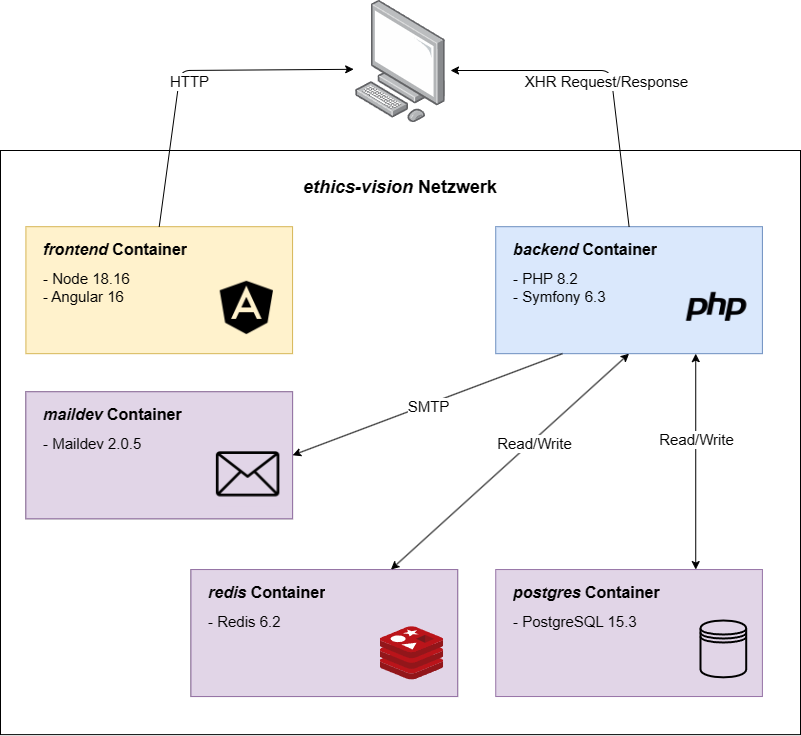
\includegraphics[width=.84\linewidth]{thesis/images/Luidold_EthicsVision-Diagramm.png}
    \caption{Übersicht des Aufbaus und der Kommunikation der EthicsVision Plattform}
    \label{fig:ethics-vision-diagramm}
\end{figure}

\subsection{Infrastruktur}
\label{sub-sec:ausarbeitung-infrastruktur}

Die EthicsVision-Plattform besteht aus zwei wesentlichen Komponenten: dem Angular-Frontend und dem Symfony-Backend.  Um sicherzustellen, dass die Anwendungen von Antragsteller:innen genutzt werden können, eine reibungslose Kommunikation und Datenübertragung stattfinden kann und eine langfristige Datenspeicherung möglich ist, ist eine entsprechende Infrastruktur erforderlich. Diese Infrastruktur erfüllt nicht nur die angesprochenen Aufgaben, sondern gewährleistet auch die Nutzbarkeit sowohl in einer Entwicklungs- als auch in einer Produktivumgebung. Das Diagramm in Abbildung \ref{fig:ethics-vision-diagramm} auf Seite \pageref{fig:ethics-vision-diagramm} veranschaulicht im Zusammenhang damit die verschiedenen Bestandteile der Plattform sowie die implementierte Infrastruktur, die mithilfe von Docker\footnote{Docker: \url{https://www.docker.com/}} realisiert wurde.

\subsubsection*{Funktionsweise von Docker}
\label{funktionsweise-docker}

Docker bietet die Möglichkeit, Applikationen und zugehörige Bestandteile unabhängig von der benötigten Infrastruktur zu entwickeln. Zeitgleich kann die Infrastruktur, ähnlich zu klassischem Quellcode, so verwaltet werden, dass standardisierte und reproduzierbare Instanzen und Umgebungen erzeugt werden können. \cite{docker_inc_docker_2023}

Docker bedient sich dabei mehrere Konzepte und Begriffe, die auch im angesprochenen Diagramm teilweise zu erkennen sind:
\begin{itemize}
    \item \textbf{Image:} Ein Image entspricht einer Vorlage, die alle Anweisungen, Abhängigkeiten und Komponenten enthält, um das Ausführen einer Anwendung in einer isolierten Umgebung zu ermöglichen. Ein Image kann dabei sowohl aus einer öffentlich zugänglichen Registry bezogen, als auch selbstständig erzeugt werden. Images bestehen typischerweise aus verschiedenen sogenannten \enquote{Layern}, bei der jede Anweisung und jedes verwendete Basis-Image einer Schicht entspricht. Werden Änderungen vorgenommen, muss lediglich der betroffene Layer aktualisiert werden, während der bestehende Cache für die anderen Schichten genutzt wird. \cite{docker_inc_docker_2023, montemagno_docker_2023}
    \item \textbf{Conainer:} Ein Container entspricht einer ausführbaren Instanz eines Image, welcher jederzeit gestartet sowie gestoppt werden kann und, ohne zusätzliche Konfiguration, isoliert ist. Der Zustand eines Containers muss explizit mittels eines Volumes persistiert werden, um wiederverwendet werden zu können. Innerhalb des Containers wird eine einzelne Applikation oder ein Service ausgeführt, der bei Bedarf mittels mehrerer Container skaliert werden kann. \cite{docker_inc_docker_2023, montemagno_docker_2023}
    \item \textbf{Volume}: Ein Volume ermöglicht es dem read-only Image (beziehungsweise dessen Instanz in Form eines Containers)  Zugriff auf das Dateisystem zu erlangen, um auch schreibende Operationen ausführen und den jeweiligen Zustand persistieren zu können. Volumes werden auf dem Host-System, auf dem Docker installiert ist, gespeichert und von Docker verwaltet. \cite{montemagno_docker_2023}
    \item \textbf{Network:} Docker Container sind, wie angesprochen, standardmäßig isoliert. Damit eine Kommunikation untereinander möglich ist, können mehrere Container in einem Netzwerk zusammengefasst werden. Die einzelnen Container wissen dabei nicht, welche anderen Container innerhalb des Netzwerks zur Verfügung stehen, da lediglich ein Netzwerk-Interface angeboten wird. Um auch eine Kommunikation mit dem Netzwerk des Host-Systems zu ermöglichen, kann für jeden Container mittels Port-Forwarding festgelegt werden, welcher Port nach außen hin freigegeben werden soll. \cite{docker_inc_networking_overview_2023}
\end{itemize}

\subsubsection*{Konkrete Anwendung von Docker im Prototyp}
\label{anwendung-docker}

Wie Abbildung \ref{fig:ethics-vision-diagramm} auf Seite \pageref{fig:ethics-vision-diagramm} zu entnehmen ist, besteht der Docker-Stack für den realisierten Prototypen aus insgesamt fünf verschiedenen Containern. Jeder Container erfüllt dabei eine spezifische Aufgabe innerhalb der EthicsVision Plattform -- mehr dazu in Abschnitt \ref{sub-sec:ausarbeitung-backend} sowie \ref{sub-sec:ausarbeitung-frontend} ab Seite \pageref{sub-sec:ausarbeitung-backend} beziehungsweise Seite \pageref{sub-sec:ausarbeitung-frontend}.

\medskip

Da die schlussendliche Applikation aus den angesprochenen fünf Anwendungen und Services besteht, kommt \textit{Docker Compose} zum Einsatz. Docker Compose stellt ein Command-Line Tool sowie ein \texttt{.yaml} Dateiformat zur Verfügung, um mehrere Images gleichzeitig starten und stoppen sowie notwendige Konfigurationen vornehmen zu können. Docker Compose erstellt zudem automatisch ein Netzwerk, das von allen Containern genutzt werden kann. \cite{montemagno_docker_2023, docker_inc_networking_compose_2023}

Quellcode \ref{code:docker-compose-excerpt} auf Seite \pageref{code:docker-compose-excerpt} zeigt einen Ausschnitt der Docker Compose Konfigurationsdatei, die für das Starten der Entwicklungsumgebung erstellt wurde. Die drei dargestellten Services umfassen sowohl den Frontend- sowie Backend-Container als auch das \ac{dbms} PostgreSQL. Gut zu erkennen ist, dass für alle drei Container jeweils ein Port-Forwarding konfiguriert wurde: Die PostgreSQL-Datenbank ist beispielsweise im Docker-Netzwerk unter dem Port \texttt{5432} erreichbar, während über das Host-System eine Verbindung über den Port \texttt{8585} aufgebaut werden kann. 

\begin{listing}[ht]
    \inputminted[fontsize=\footnotesize,linenos,xleftmargin=8mm]{yaml}{code/Luidold_Docker-Compose.yml}
    \caption{Auszug aus dem \texttt{docker-compose.development.yml} der EthicsVision Plattform}
    \label{code:docker-compose-excerpt}
\end{listing}

Ebenso lässt sich erkennen, dass dem \texttt{postgres} Container ein Volume zugewiesen wurde, um die in der Datenbank gespeicherten Daten permanent persistieren und wiederverwenden zu können. Für die Datenbank wird das in einer Docker Registry veröffentliche \texttt{postgres} Image herangezogen, während das Image für den \texttt{frontend} und \texttt{backend} Container jeweils einer eigenen Umsetzung entspricht.\footnote{In allen drei Images kommen Variablen vor, die außerhalb der Docker Compose Konfigurationsdatei in einer \texttt{.env} Datei angegeben wurden, um die Wartung der eingesetzten Versionen und des Projektnamens zu zentralisieren.}

\medskip

Quellcode \ref{code:docker-compose-commands} auf Seite \pageref{code:docker-compose-commands} zeigt, wie der Docker-Stack mittels Docker Compose gestartet und gestoppt werden kann. Um das häufig vorkommende Starten und Stoppen zu vereinfachen, findet im umgesetzten Projekt ein Makefile Anwendung, welches die Befehle noch einmal vereinfacht und die Nutzung von Umgebungsvariablen unterstützt.\footnote{Siehe \url{https://github.com/DominicLuidold/ethics-vision/blob/main/Makefile}}.

\begin{listing}[ht]
    \inputminted[fontsize=\footnotesize,linenos,xleftmargin=8mm]{bash}{code/Luidold_Docker-Compose-Commands.sh}
    \caption{Docker Compose Befehle zum Starten und Stoppen des EthicsVision Docker-Stacks}
    \label{code:docker-compose-commands}
\end{listing}

\subsubsection*{Individuelle Docker Images}
\label{sub-sub-sec:individuelle-docker-images}

Wie in Quellcode \ref{code:docker-compose-excerpt} auf Seite \pageref{code:docker-compose-excerpt} deutlich wird, nutzen die \texttt{frontend} und \texttt{backend} Container jeweils eigens erstellte Docker Images. Neben den Basis-Images (\texttt{node: 18.16-alpine} für den Frontend"=Container und \texttt{php:8.2-fpm-bullseye} für den Backend"=Container) werden spezifische Abhängigkeiten und Komponenten installiert, um die Ausführung der Anwendungen zu ermöglichen. Konkret wird für die Angular"=Anwendung das \texttt{@angular/cli} Package installiert, während für die Symfony-Anwendung verschiedene PHP-Erweiterungen, wie zum Beispiel \texttt{pdo\_pgsql}, hinzugefügt und zusätzliche Konfigurationsdateien kopiert werden.

\subsubsection*{Entscheidung für Docker \& langfristige Implikationen}
\label{sub-sub-sec:entscheidung-docker}

Die Entscheidung, die gesamte Applikation auf einem Technologie-Stack basierend auf mehreren Containern aufzubauen, wurde aus verschiedenen Gründen getroffen. Einerseits beruht die Entscheidung auf dem technischen Hintergrund von Docker und seiner konkreten Anwendungsmöglichkeiten, dass sowohl die Entwicklung als auch der potenzielle Einsatz der Applikation in einer Produktivumgebung abgebildet werden können. Andererseits ermöglicht der gegenwärtige Stand des Prototyps die Installation auf jedem Docker-kompatiblen Host-System, ohne dass die betreffenden Services direkt auf dem Host-System selbst installiert werden müssen. Zusätzlich ermöglicht dieser Ansatz im weiteren Verlauf eine spezifische Konfiguration für den Einsatz in einer produktiven Umgebung, in der häufig unterschiedliche Anforderungen an Konfigurationen und Skalierung der Services bestehen.

\subsection{Backend}
\label{sub-sec:ausarbeitung-backend}

Das sogenannte \enquote{Backend} hat im Kontext der EthicsVision Plattform mehrere Aufgaben, die aus technischer Sicht mit dem Symfony-Framework, dem \ac{dbms} PostgreSQL sowie einigen Patterns und Konzepten realisiert wurden. Zu den Aufgaben gehören
\begin{itemize}
    \item das Bereitstellen von Formularen und Formular"=Einträgen im Kontext des Ethikantrages,
    \item die Möglichkeit, Formulare und Formular"=Einträge zu erstellen, zu bearbeiten und zu löschen sowie
    \item der Versand von Benachrichtigungen in Form von E-Mails bei Eintreten spezifischer Ereignisse.
\end{itemize}

Um einen Überblick über die Herangehensweise zu ermöglichen, werden im Folgenden der Aufbau der Datenstruktur, das Symfony-Framework als Grundlage, die angewandten Patterns sowie die verwendete Infrastruktur genauer beleuchtet.

\subsubsection*{Datenstruktur}
\label{sub-sub-sec:backend-datenstruktur}

Als erster Schritt der Entwicklung wurde der bestehende Ethikantrag herangezogen, um eine grundlegende Datenstruktur und vor allem eine auf Softwareebene umsetzbare Abbildung davon auszuarbeiten. Im Zuge dieses Schrittes wurde der Fokus jedoch nicht rein auf den in dieser Arbeit behandelten Ethikantrag gelegt, sondern breiter gesetzt, um die grundlegend ähnlichen Komponenten eines Antrages sowie Formulares herauszuarbeiten. Dadurch soll der Prototyp bei Bedarf auch für anderweitige, zukünftige Formulare der \ac{fek} oder gänzlich andere Einsatzzwecke verwendet werden können.

Unter Zuhilfenahme der in Abschnitt \ref{sec:inhaltlicher-aufbau} ab Seite \pageref{sec:inhaltlicher-aufbau} durchgeführten Analyse der Word"=Antragsvorlage konnten die folgenden Kernelemente identifiziert werden, die in Folge dessen die Domänenschicht im Backend sowie die Darstellung im Frontend maßgeblich vorgeben:
\begin{itemize}
    \item \textbf{Element:} Die kleinste Einheit in einem Formular beziehungsweise dem Ethikantrag stellt ein einzelnes Textfeld, ein Kontrollkästchen oder ein anderweitiges Konstrukt dar, mit dem Antragsteller:innen aktiv interagieren müssen. Diese Bestandteile eines Formulars werden in der Umsetzung des Prototyps \textit{Element} genannt. Ein Element besitzt dabei sowohl einen Titel (sprich eine konkrete Frage oder eine Aussage), eine Ausprägung (ein Textfeld oder ähnliches) sowie eine optionale Beschreibung, eine Position innerhalb der übergeordneten Section und einen möglichen Platzhalter.
    \item \textbf{Section:} Die nächst größere Einheit, die im Ethikantrag und oftmals ebenso in anderweitigen Formularen vorkommt, sind thematische Blöcke, in die die einzelnen Fragen beziehungsweise Elemente aufgeteilt sind. Diese thematischen Blöcke, sogenannte \textit{Section}s, gruppieren zusammengehörige Elemente und verfügen ebenso über einen Titel, eine optionale Beschreibung sowie eine Position innerhalb des Formulars.\\
    Um den Ethikantrag und anderweitige Formulare im weiteren Verlauf an spezifische Gegebenheiten anpassen und gewisse Fragen ein- und ausblenden zu können, werden für jede Section zusätzlich Meta"=Informationen definiert, die aussagen, zu welchem thematischen Block diese zugehörig sind.
    \item \textbf{Screen:} Um die Möglichkeit zu schaffen, Antragsteller:innen zusätzliche Informationen bereitzustellen, bevor mit der Beantwortung von Fragen begonnen wird und nachdem das Formular vollständig ausgefüllt wurde, werden zwei sogenannte \textit{Screen}s eingeführt. Diese haben jeweils einen Titel sowie einen Inhalt und sind Teil des in Abschnitt \ref{sec:erläuterung-konzept} ab Seite \pageref{sec:erläuterung-konzept} angesprochenen Formular-Assistenten.
    \item \textbf{Form:} Als abschließende Einheit fungiert im \ac{poc} das \textit{Form}, welches die Screens und Sections (und somit die einzelnen Elemente) enthält und ebenfalls über einen Titel sowie eine Beschreibung verfügt.
\end{itemize}

Um neben der Definition eines Formulars auch konkrete Einreichungen und übermittelte Daten der Antragsteller:innen abbilden zu können, wurden zwei weitere Konzepte ausgearbeitet, die diese Funktionalität abbilden:
\begin{itemize}
    \item \textbf{Entry:} Ein eingereichtes Formular wird in der Umsetzung \textit{Entry} genannt und enthält neben verschiedenen Zeitstempeln zur Erstellung, letzten Aktualisierung und Einreichung auch einen Status (konkret \texttt{Offen} oder \texttt{Eingereicht}).\\
    Ähnlich zur Section werden auch für einen Eintrag Meta"=Informationen gespeichert, um später reproduzieren zu können, welche konkreten Sections mit dem Formular-Assistenten ausgewählt wurden, um das generierte Formular an die Projektumstände anzupassen.
    \item \textbf{ElementEntry:} Jeder Entry besteht aus sogenannten \textit{ElementEntry}s, die eine konkrete Verknüpfung zu einem Element besitzen und den eingegeben Wert beinhalten.
\end{itemize}

\subsubsection*{Domänenschicht}
\label{sub-sub-sec:backend-domänenschicht}

Die Domänenschicht basiert auf der definierten Datenstruktur und enthält zeitgleich entsprechende Logik, um Ethikanträge der \acl{fek} der \acl{fhv} abbilden zu können. Wie bereits angesprochen, ist in Abbildung \ref{fig:ethics-vision-uml} auf Seite \pageref{fig:ethics-vision-uml} ersichtlich, dass der Bezug zu einem Ethikantrag nur indirekt gegeben ist und die \texttt{Form} Klasse stattdessen eine zentrale Rolle einnimmt. Alle anderen Klassen hängen sowohl direkt als auch indirekt von ihr ab, was auch durch die eingezeichneten Kompositionen als Relationen zwischen den Klassen verdeutlicht wird.

\begin{figure}[ht]
    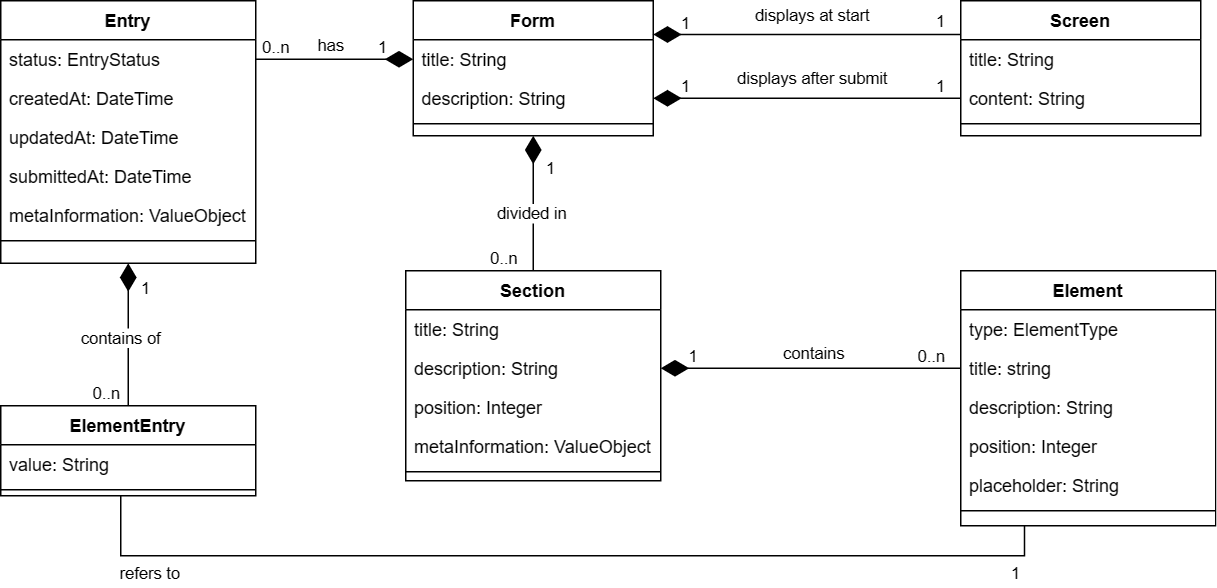
\includegraphics[width=\linewidth]{thesis/images/Luidold_EthicsVision-Klassendiagramm.png}
    \caption{Vereinfachtes UML"=Klassendiagramm der EthicsVision Domäne}
    \label{fig:ethics-vision-uml}
\end{figure}

Die Modellierung der Domänenschicht und auch der als Basis dienenden Datenstruktur orientiert sich an den Prinzipien des \acp{ddd}, die zumindest in grundlegender Form\footnote{Aufgrund des Fokus auf die schnelle Entwicklung eines ersten Prototyps und der überschaubaren Komplexität des Systems wurden nicht alle Konzepte des \ac{ddd} konsequent übernommen.} Anwendung gefunden haben.

Im Bereich des \ac{ddd} nimmt das Verständnis der Prozesse, die mittels einer Software"=Lösung abgebildet werden sollen, eine essenzielle Rolle ein. Die Domäne, in der diese Prozesse stattfinden und in der eine Applikation schlussendlich verwendet wird, stellt den Kontext bereit, in dem Aktionen ausgeführt und Daten bereitgestellt sowie validiert werden. Zusätzlich dazu bringt die Domäne eine \textit{Ubiquitous Language}, eine einheitliche Sprache, mit sich, die von Anwender:innen und Entwickler:innen genutzt werden kann, um für beide Seiten verständliche Begrifflichkeiten zu definieren und zu verwenden. \cite{airbrake_technologies_inc_domain-driven_2022, fowler_domaindrivendesign_2020}

Innerhalb des \ac{ddd}-Konzepts kommen zudem unterschiedliche Abstraktionen zur Anwendung, wie beispielsweise \textit{Entities}, \textit{Value Objects} und \textit{Aggregates} sowie \textit{Aggregate Roots}. Aggregate Roots nehmen eine zentrale Rolle ein, da sie als Anlaufstellen für die Ausführung und Validierung von domänenspezifischen Aktionen und Methoden genutzt werden -- die \texttt{Form} Klasse ist ein Beispiel dafür. Aggregates sind verantwortlich für die Zusammenfassung mehrerer Entities innerhalb eines definierten \textit{Bounded Contexts}. Value Objects haben die Aufgabe, Daten in unveränderlicher Form zu halten. \cite{airbrake_technologies_inc_domain-driven_2022, fowler_domaindrivendesign_2020, fowler_ddd_aggregate_2013}

\medskip

Quellcode \ref{code:form-aggregate-root} auf Seite \pageref{code:form-aggregate-root} bezieht sich auf ausgewählte Methodensignaturen der \texttt{Form} Klasse, welche verdeutlichen, dass die Klasse hauptverantwortlich für das Erstellen und Verwenden von Formularen sowie den zugehörigen \texttt{Section} und \texttt{Element} Objekten ist. Trotz ihrer Auslegung als Aggregate Root ist die Klasse jedoch nicht für das Erstellen und Bearbeiten von \texttt{Entry} und \texttt{ElementEntry} Objekten zuständig. Diese Vorgehensweise wurde gewählt, um in zukünftigen Versionen eine Entkopplung von \texttt{Entry} Objekten von \texttt{Form} Objekten und deren Abhängigkeiten zu erleichtern. Dadurch könnten Einreichungen weiterhin bestehen bleiben, selbst wenn Formulare oder einzelne Elemente geändert oder gelöscht werden, was derzeit noch nicht möglich ist.

\begin{listing}[ht]
    \inputminted[fontsize=\footnotesize,linenos,xleftmargin=8mm]{php}{code/Luidold_Form-Aggregate-Root.php}
    \caption{Ausgewählte Methoden"=Signaturen der \texttt{Form} Aggregate Root Klasse der EthicsVision Plattform}
    \label{code:form-aggregate-root}
\end{listing}

\subsubsection*{Aufbau der Symfony-Applikation}
\label{sub-sub-sec:aufbau-symfony-applikation}

Das Symfony-Framework wurde als technische Grundlage für die Umsetzung des Backends gewählt, da mit dem Framework und den dafür zur Verfügung stehenden First-Party sowie Third-Party Erweiterungen, regelmäßigen Updates und einer detaillierten Dokumentation eine Vielzahl an Möglichkeiten zur Verfügung stehen, die definierten Anforderungen umsetzen zu können. Daneben ermöglicht das Symfony-Framework mit seiner \acl{mvc} Architektur eine saubere Trennung der unterschiedlichen Schichten einer modernen Applikation und bietet gleichzeitig die Möglichkeit, den Projektgegebenheiten angepasst und bei Bedarf erweitert zu werden. Wie bereits in Abschnitt \ref{sec:ausarbeitung-wahl-technische-basis} ab Seite \pageref{sec:ausarbeitung-wahl-technische-basis} angesprochen wurde, eignet sich das Symfony-Framework zudem, um eine vom \acl{ui} entkoppelte Applikation umzusetzen, die bei Bedarf ebenso in andere Systemen integriert werden kann. \cite{symfony_sas_six-reasons_2023, kszczanowicz_why_2021} 

In der Umsetzung des \ac{poc} wird Symfony konkret in der Version \texttt{6.3} mit PHP \texttt{8.2} betrieben, was jeweils den aktuellsten Versionen zum Zeitpunkt dieser Arbeit im Sommersemester 2023 entspricht. Zum Einsatz kommen dabei zudem \textit{Composer}\footnote{Composer: \url{https://getcomposer.org/}} für die Verwaltung von Abhängigkeiten und verwendeten Paketen sowie unter anderem \textit{Doctrine}\footnote{Doctrine: \url{https://www.doctrine-project.org/}} als \ac{orm} Tool sowie Schnittstelle zwischen Applikation und Datenbank.

\medskip

Wie in Abbildung \ref{fig:ethics-vision-api-docs} auf Seite \pageref{fig:ethics-vision-api-docs} zu sehen ist, stellt der Hauptbestandteil der mit Symfony umgesetzten Backend-Anwendung das \ac{api} dar, mit der beliebige \ac{ui}-Umsetzungen auf die verschiedenen Funktionalitäten und Operationen des Systems zugreifen können. Die in der Abbildung aufgelisteten Endpunkte können dabei im realisierten Prototypen ohne Authentifizierung angesteuert werden und sind nach dem Prinzip des \acp{rest} stateless. \cite{gupta_stateless_2018}

\begin{figure}[ht]
    \centering
    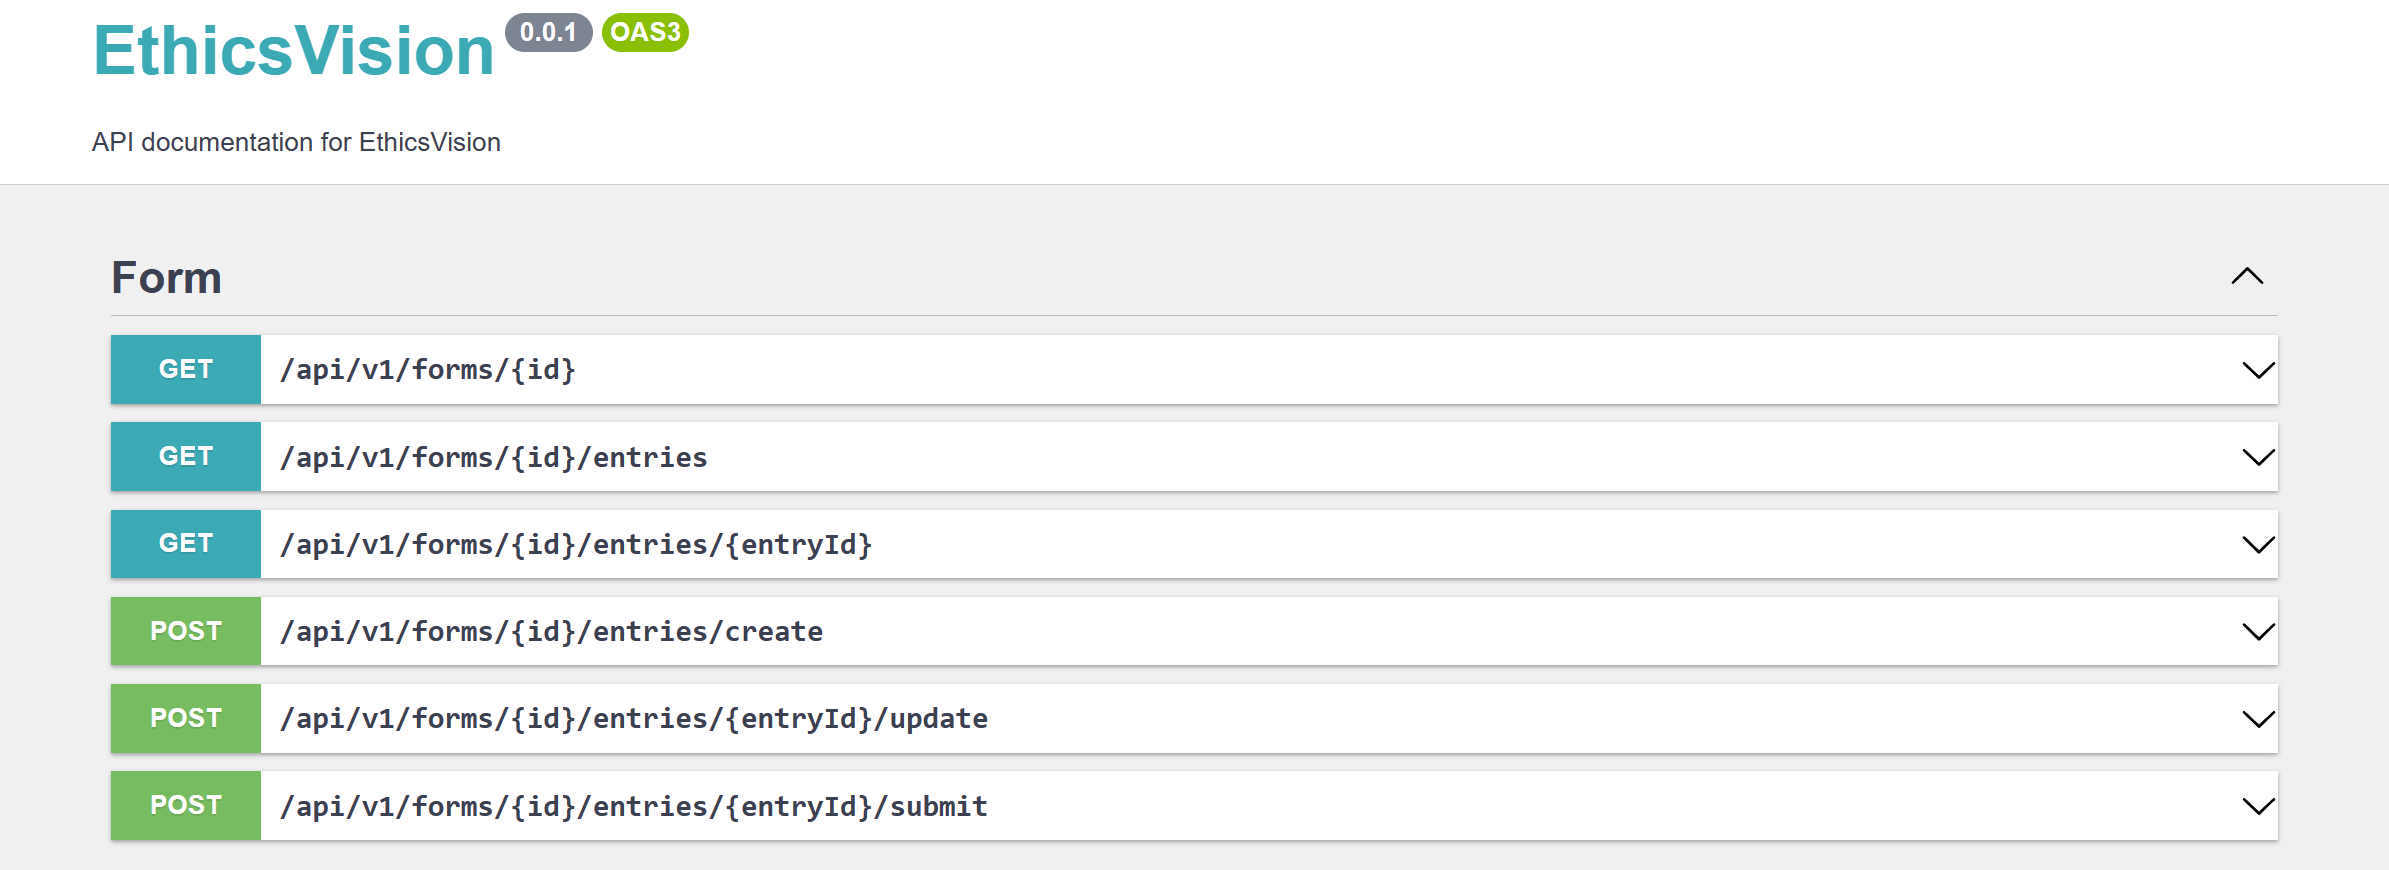
\includegraphics[width=\linewidth]{thesis/images/Luidold_EthicsVision-API-Docs.png}
    \caption{\acs{api}-Dokumentation der EthicsVision Plattform}
    \label{fig:ethics-vision-api-docs}
\end{figure}

Die Applikation rund um die insgesamt sechs Endpunkte ist intern in die drei Schichten der \ac{mvc}-Architektur aufgeteilt:
\begin{itemize}
    \item \textbf{Model:} Das Model entspricht der Domänenschicht, die in diesem Abschnitt bereits ausführlich erläutert wurde und enthält die Aggreagate Roots und Entities im Kontext des \ac{ddd}. Diese werden von Doctrine im Rahmen des \ac{orm} als Entities mit Daten angereichert. Der Zugriff auf die Datenbank, um mit den angereicherten Objekten in der Applikationslogik interagieren zu können, wird dabei durch sogenannte \textit{Repositories} ermöglicht. Diese befinden sich, zusammen mit den zugehörigen \ac{orm}-Konfigurationsdateien im \texttt{XML}-Format, in einem separaten Namespace\footnote{Die Domänenschicht befindet sich im \url{App\\Form\\Domain\\Model} Namespace, während die konkreten Implementierungen der Repositories in \url{App\\Form\\Infrastructure\\Repository} zu finden sind.}, um eine Vermischung der Schichten zu verhindern.
    \item \textbf{View:} In der Umsetzung des \aclp{poc} wird die View"=Schicht über mehrere \acp{dto} realisiert, die von den verschiedenen \ac{api}-Endpunkten als serialisierte \ac{json} Objekte zurückgegeben werden.
    \item \textbf{Controller:} In ähnlicher Weise zur View-Schicht nutzen die umgesetzten \textit{Controller} vom Framework bereitgestellte, deserialisierte \ac{json}-Objekte in Form von \ac{dto}s, die zusätzlich validiert werden. Die in den \acp{dto}s enthaltenen Daten werden im weiteren Verlauf dabei nicht direkt von den jeweiligen Controllern verarbeitet, sondern, wie von \cite{symfony_sas_best-practices_2023} empfohlen, an dedizierte \textit{Command-} und \textit{QueryHandler} delegiert.
\end{itemize}

\clearpage

Quellcode \ref{code:form-controller} auf Seite \pageref{code:form-controller} zeigt beispielhaft jene Methode des \texttt{FormController}s, die für die Erstellung eines neuen Eintrags für ein Formular zuständig ist. Die Methode nimmt dabei den \texttt{CreateEntryCommand} entgegen, delegiert diesen an den dafür zuständigen CommandHandler und retourniert das bereitgestellte Ergebnis in Form einer \ac{json}-Response.

\begin{listing}[ht]
    \inputminted[fontsize=\footnotesize,linenos,xleftmargin=8mm,breaklines]{php}{code/Luidold_Form-Controller.php}
    \caption{Ausschnitt des \texttt{FormController}s der EthicsVision Plattform}
    \label{code:form-controller}
\end{listing}

Das hierbei angewandte und stellenweise auch schon angedeutete Pattern basiert auf den Prinzipien der \ac{cqrs}. Die Begriffe \textit{Command} und \textit{Query}, die ursprünglich auf die \ac{cqs} zurückgehen, definieren dabei Zugriffsarten, bei denen lesende und schreibende Aktionen explizit von einander getrennt werden: \cite{noauthor_cqrs_2010, fowler_commandqueryseparation_2005}, \cite[238\psq]{ingeno_software_2018}

\begin{itemize}
    \item \textbf{Query:} Lesende Operationen werden in Form von Queries durchgeführt, um auf die Daten eines Systems zuzugreifen, ohne diese oder den Systemzustand zu verändern. In der konkreten Umsetzung werden, wie angesprochen, QueryHandler verwendet, die von Symfony über die \texttt{symfony/messenger} Komponente verarbeitet werden. \cite{fowler_commandqueryseparation_2005} \cite[238\psq]{ingeno_software_2018}
    \item \textbf{Command:} Schreibende Operationen hingegen werden in Form von Commands ausgeführt und führen zu Änderungen der Daten und des Systemzustands mit potenziellen Seiteneffekten. Laut Definition liefern Commands beziehungsweise CommandHandler, die sowohl synchron als auch asynchron ausgeführt werden können, kein Ergebnis zurück. Im vorliegenden \texttt{FormController} werden jedoch bestimmte Daten vom Angular-Frontend benötigt, die daher direkt als Ergebnis bereitgestellt werden. \cite{fowler_commandqueryseparation_2005} \cite[238\psq]{ingeno_software_2018}
\end{itemize}

Der \ac{cqrs}-Ansatz wurde gewählt, da dieser mehrere Vorteile in verschiedenen Bereichen bietet: Durch die gezielte Aufteilung von lesenden und schreibenden Aktionen kann die Wartbarkeit, Erweiterbarkeit und Flexibilität eines Systems verbessert werden. Zudem ermöglicht dieser Ansatz eine präzisere Implementierung von Funktionen, bei denen die Sicherheit (\textit{Security} im Englischen) und damit verbundene Aspekte eine Rolle spielen, da lesende und schreibende Operationen voneinander getrennt sind. Auch kann eine Steigerung der Performance erreicht werden, indem die verschiedenen Operationen unterschiedlich skaliert werden. Die Vorteile, wie von \cite{ingeno_software_2018} erwähnt, kommen dabei vor allem komplexeren Systemen zugute. Der implementierte Prototyp ist dadurch jedoch bereits darauf ausgelegt, mögliche Weiterentwicklungen mit weniger Hindernissen hinsichtlich Größe und Komplexität zu bewältigen (vgl. \cite[240]{ingeno_software_2018}).

\subsubsection*{Genutzte Infrastruktur}
\label{sub-sub-sec:backend-genutzte-infrastruktur}

- Postgres
- Redis
- Maildev

\subsection{Frontend}
\label{sub-sec:ausarbeitung-frontend}

\chapter{Evaluation des Prototyps}
\label{chap:evaluation-prototyp}

% Literaturverzeichnis
\clearpage
\phantomsection
\addcontentsline{toc}{chapter}{Literaturverzeichnis}
\printbibliography

% Anhang
\appendix

\chapter{Eingereichter Ethikantrag}
\label{appendix:eingereichter-ethikantrag}

Anhang \ref{appendix:eingereichter-ethikantrag} enthält den im Rahmen dieser Masterarbeit ausgearbeiteten Ethikantrag, welchem -- neben dem konkreten Antrag selbst -- Anhang \ref{appendix:ursprünglicher-leitfaden} sowie Anhang \ref{appendix:ursprüngliches-informed-consent-formular} ab Seite \pageref{appendix:ursprünglicher-leitfaden} beziehungsweise ab Seite \pageref{appendix:ursprüngliches-informed-consent-formular} angehängt wurden.

Der fertiggestellte Antrag wurde am Freitag, den 03.03.2023, fristgerecht an den Vorsitz der \acl{fek} der \acl{fhv} mittels E-Mail übermittelt, um in der \ac{fek} Sitzung vom Mittwoch, den 22.03.2023, behandelt werden zu können.

\medskip 

Anhang \ref{appendix:rückmeldung-fek} ab Seite \pageref{appendix:rückmeldung-fek} spiegelt die Rückmeldung der \ac{fek} inklusive des abschließenden ethischen Votums wider, welche in der angesprochenen Sitzung der Kommission ausgearbeitet wurde. Anhang \ref{appendix:interview-leitfaden} ab Seite \pageref{appendix:interview-leitfaden} sowie Anhang \ref{appendix:informed-consent-einzelinterview} und Anhang \ref{appendix:informed-consent-gruppendiskussion} ab Seite \pageref{appendix:informed-consent-einzelinterview} beziehungsweise \pageref{appendix:informed-consent-gruppendiskussion} stellen die überarbeiteten Versionen des Leitfadens und der Einwilligungserklärungen dar, die anhand des Feedbacks der Kommission adaptiert und ausgearbeitet wurden.

\subsubsection*{Anmerkungen}
\label{appendix:anmerkungen-eingereichter-ethikantrag}
Die übermittelte Version des Ethikantrages wurde sowohl von Karin Trommelschläger, MSc in der Funktion als Betreuerin dieser Masterarbeit als auch vom Antragsteller unterschrieben. Neben der Schwärzung der E-Mail-Adresse und der Telefonnummer wurden die Unterschriften in der angehängten Version für eine verbesserte Lesbarkeit entfernt.

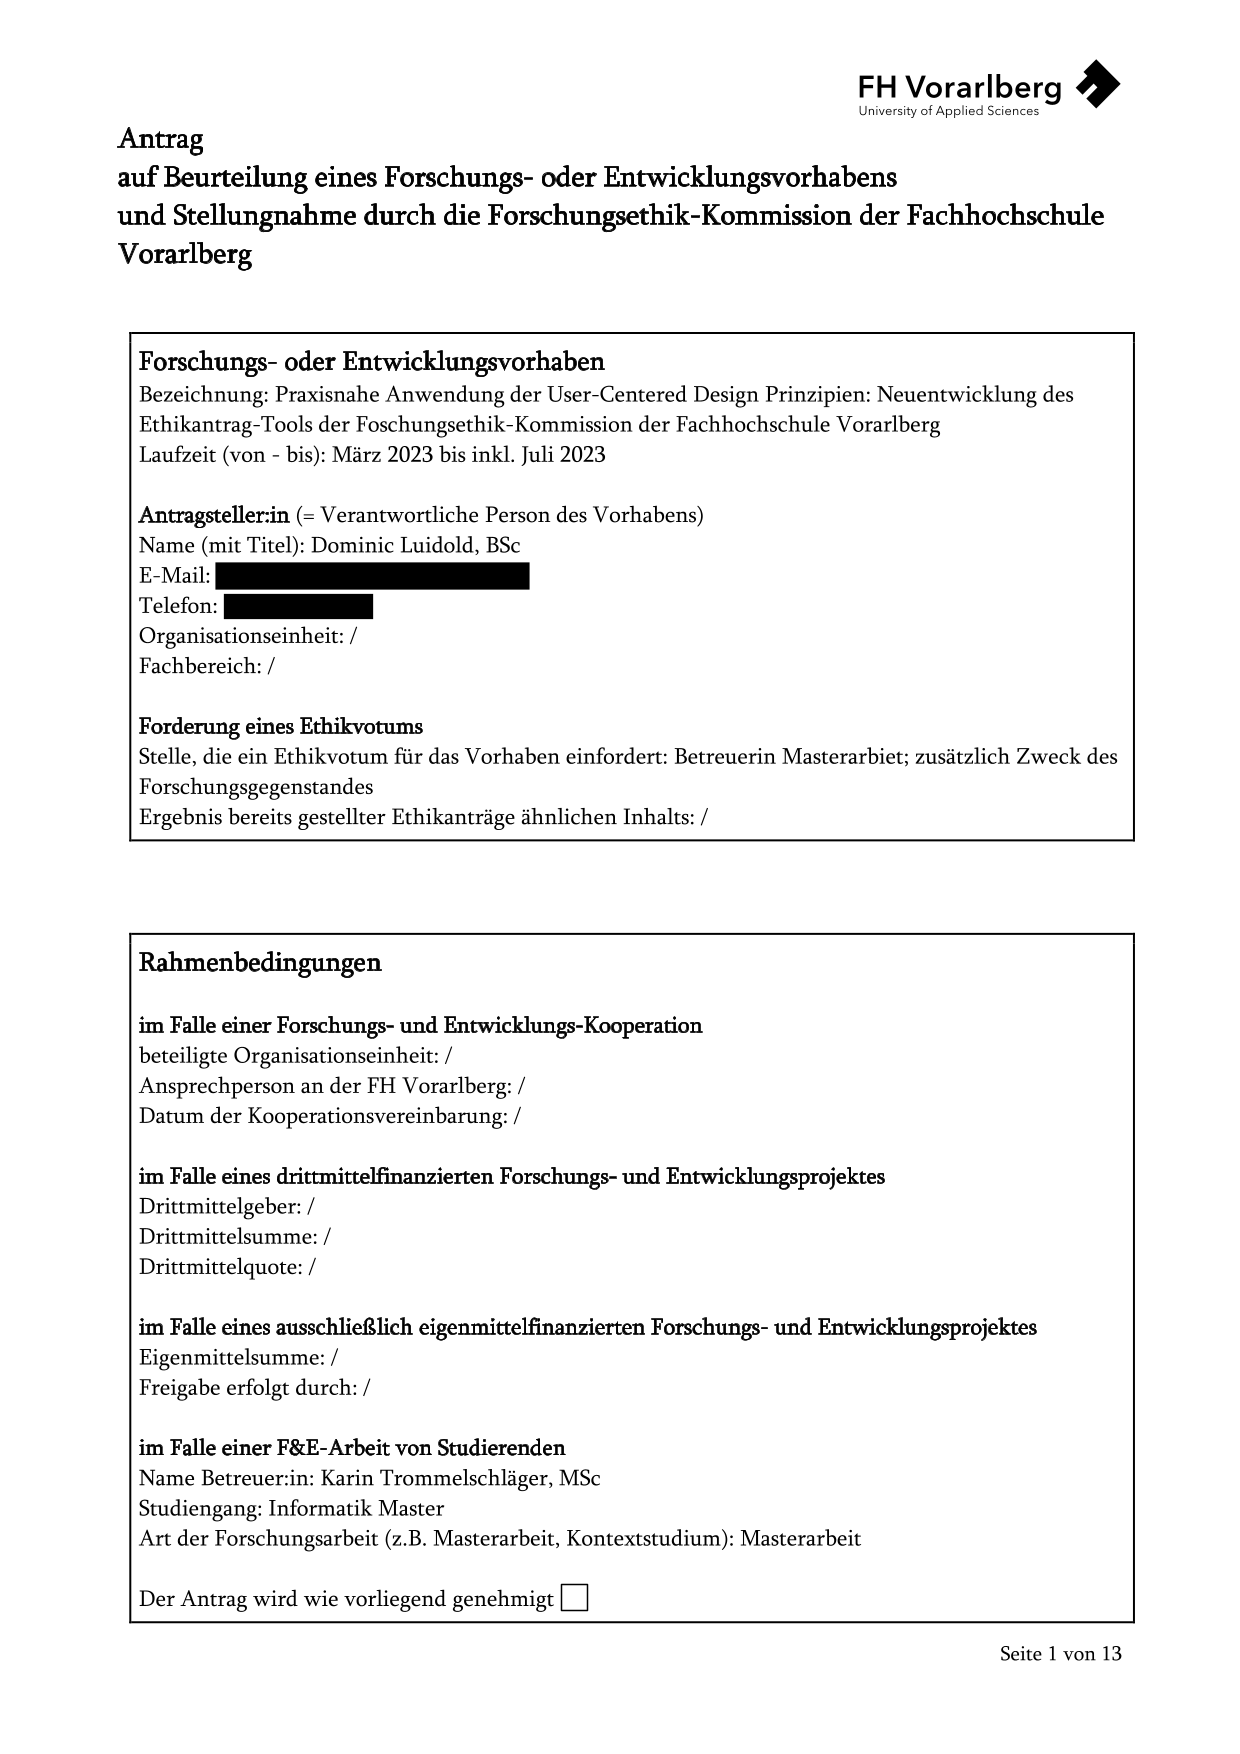
\includepdf[pages=-]{documents/Luidold_Ethikantrag.pdf}

\chapter{Eingereichter Leitfaden für Interviews \& Fragebögen}
\label{appendix:ursprünglicher-leitfaden}

Anhang \ref{appendix:ursprünglicher-leitfaden} enthält die ursprüngliche Fassung des Leitfadens, welcher die Fragen für die anfangs geplanten Interviews und Fragebögen enthalten hat und im Rahmen des Ethikantrages (siehe Anhang \ref{appendix:eingereichter-ethikantrag} ab Seite \pageref{appendix:eingereichter-ethikantrag}) der \acl{fek} der \acl{fhv} übermittelt wurde.

\medskip

Anhang \ref{appendix:interview-leitfaden} ab Seite \pageref{appendix:interview-leitfaden} stellt die schlussendliche angewandte Fassung des Leitfadens dar, welcher anhand des Feedbacks der \ac{fek} überarbeitet und adaptiert wurde.

\includepdf[pages=-]{documents/Luidold_Ursprünglicher-Leitfaden-Interview-Fragebogen.pdf}

\chapter{Eingereichtes Formular zur Einwilligungserklärung}
\label{appendix:ursprüngliches-informed-consent-formular}

Anhang \ref{appendix:ursprüngliches-informed-consent-formular} enthält die ursprüngliche Fassung der Einwilligungserklärung, die sowohl für die Durchführung der Interviews als auch der Fragebögen angedacht war und im Rahmen des Ethikantrages (siehe Anhang \ref{appendix:eingereichter-ethikantrag} ab Seite \pageref{appendix:eingereichter-ethikantrag}) der \acl{fek} der \acl{fhv} übermittelt wurde.

\medskip

Anhang \ref{appendix:informed-consent-einzelinterview} ab Seite \pageref{appendix:informed-consent-einzelinterview} sowie Anhang \ref{appendix:informed-consent-gruppendiskussion} ab Seite \pageref{appendix:informed-consent-gruppendiskussion} stellen die schlussendliche angewandten Fassungen der Einwilligungserklärungen dar, welche anhand des Feedbacks der \ac{fek} überarbeitet und adaptiert wurden.

\includepdf[pages=-]{documents/Luidold_Ursprüngliches-Informed-Consent-Formular.pdf}

\chapter{Rückmeldung der \acl{fek} zum eingereichten Ethikantrag}
\label{appendix:rückmeldung-fek}

Anhang \ref{appendix:rückmeldung-fek} enthält die Rückmeldung sowie das ethische Votum der \acl{fek} der \acl{fhv}, welches in der Sitzung vom Mittwoch, den 22.03.2023, auf Einlangen des eingereichten Ethikantrages (siehe Anhang \ref{appendix:eingereichter-ethikantrag} ab Seite \pageref{appendix:eingereichter-ethikantrag}) hin erstellt wurde.

\medskip

Als Resultat der Rückmeldung und des Feedbacks der \ac{fek} wurde eine adaptierte und überarbeitete Version des Interviewleitfadens (siehe Anhang \ref{appendix:interview-leitfaden} ab Seite \pageref{appendix:interview-leitfaden}) sowie zwei neue beziehungsweise überarbeitete Einwilligungserklärungen (siehe Anhang \ref{appendix:informed-consent-einzelinterview} und Anhang \ref{appendix:informed-consent-gruppendiskussion} ab Seite \pageref{appendix:informed-consent-einzelinterview} beziehungsweise \pageref{appendix:informed-consent-gruppendiskussion}) erstellt. Eine detaillierte Auflistung der vorgenommenen Änderungen findet sich bei den jeweiligen Anhängen.

\subsubsection*{Anmerkungen}
\label{appendix:anmerkungen-rückmeldung-fek}

Siehe Abschnitt \ref{sec:angewandter-kriterienkatalog} ab Seite \pageref{sec:angewandter-kriterienkatalog} für eine Erklärung zur Bewertung zweier Kriterien des Kriterienkataloges (Seite 3 der Rückmeldung) sowohl mit \enquote{Stufe I} als auch mit \enquote{Stufe II}.


\includepdf[pages=-]{documents/Forschungsethik-Kommission-FHV_Votum-Ethikantrag.pdf}

\chapter{Adaptierter und angewandter Interviewleitfaden}
\label{appendix:interview-leitfaden}

Anhang \ref{appendix:interview-leitfaden} enthält die adaptierte und überarbeitete Fassung des Interviewleitfadens, welcher auf Anhang \ref{appendix:ursprünglicher-leitfaden} ab Seite \pageref{appendix:ursprünglicher-leitfaden} basiert. Der Leitfaden wurde Anhand der Rückmeldung und des Feedbacks der \acl{fek} der \acl{fhv} (siehe Anhang \ref{appendix:rückmeldung-fek} ab Seite \pageref{appendix:rückmeldung-fek}) angepasst.

\subsubsection*{Durchgeführte Änderungen}
\label{appendix:änderungen-interview-leitfaden}

Folgende Änderungen wurden im Vergleich zur ursprünglichen Variante vorgenommen:
\begin{itemize}
    \item Der Abschnitt \textit{Fragebogenfragen -- Forschende [die (k)einen Ethikantrag gestellt haben, sich gerade im Prozess der Antragsstellung befinden oder sich gegen einen Antrag entschieden haben]} wurde gänzlich entfernt
    \item Der Abschnitt \textit{Fragebogenfragen -- Master-Studierende} wurde gänzlich entfernt
    \item Im Abschnitt \textit{Interviewfragen -- Forschende [die bereits einen Ethikantrag gestellt haben]} wurde eine Frage angepasst und drei neue Fragen hinzugefügt
\end{itemize}

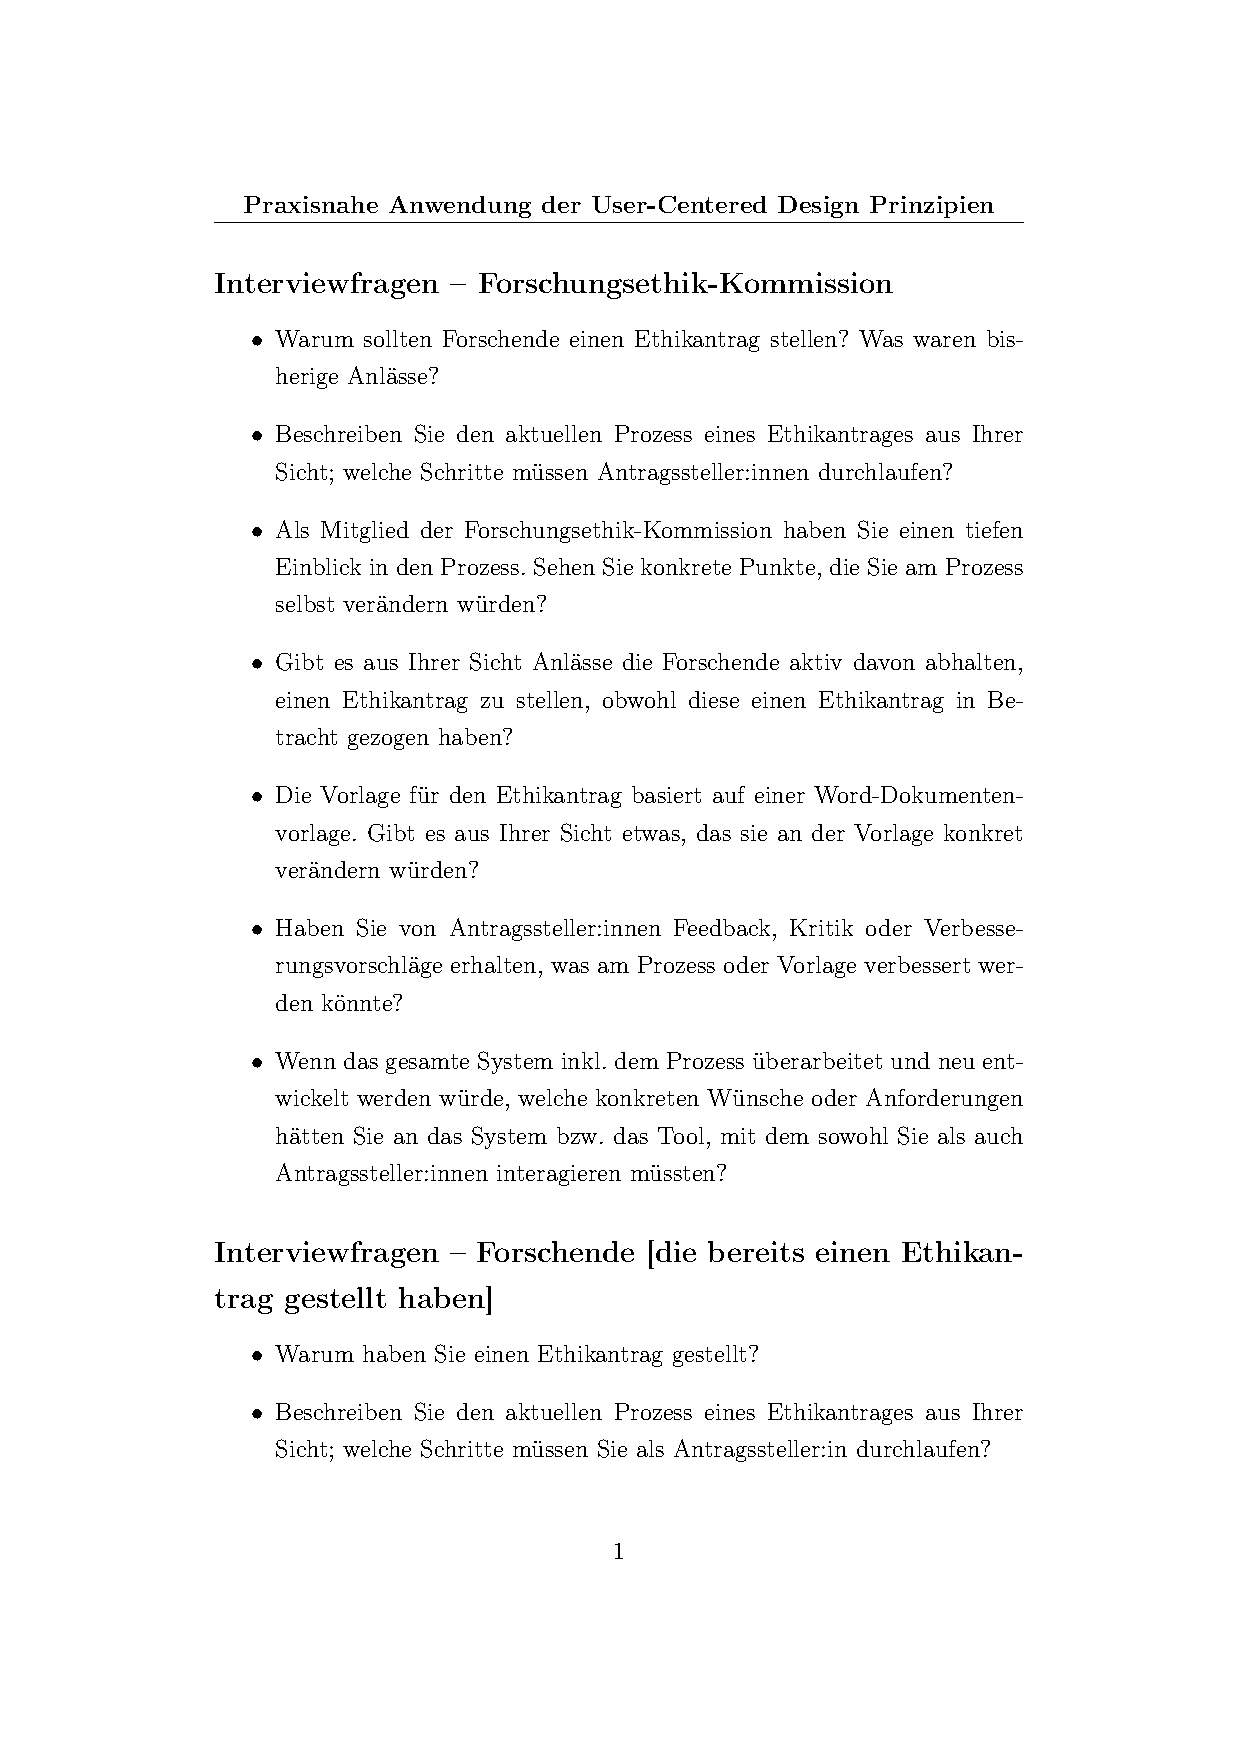
\includepdf[pages=-]{documents/Luidold_Interviewleitfaden.pdf}

\chapter{Einwilligungserklärung zur Teilnahme an einem Einzelinterview}
\label{appendix:informed-consent-einzelinterview}

Anhang \ref{appendix:informed-consent-einzelinterview} enthält die auf Basis von Anhang \ref{appendix:ursprüngliches-informed-consent-formular} ab Seite \pageref{appendix:ursprüngliches-informed-consent-formular} neu geschaffene Einwilligungserklärung für Einzelinterviews. Die Einwilligungserklärung wurde Anhand der Rückmeldung und des Feedbacks der \acl{fek} der \acl{fhv} (siehe Anhang \ref{appendix:rückmeldung-fek} ab Seite \pageref{appendix:rückmeldung-fek}) konkretisiert.

\subsubsection*{Durchgeführte Änderungen}
\label{appendix:änderungen-informed-consent-einzelinterview}

Folgende Änderungen wurden im Vergleich zur ursprünglichen Variante vorgenommen:
\begin{itemize}
    \item Der Titel des Dokumentes wurde präzisiert, sodass klar ist, dass es sich um eine Einwilligung für ein Einzelinterview handelt
    \item Im Abschnitt \textit{Zustimmung zur Verarbeitung der Daten} wurde präzisiert, dass die Datenerhebung im Rahmen eines Einzelinterviews stattfindet
    \item Im Abschnitt \textit{Einwilligung} wurde die Einwilligung zur Tonbandaufzeichnung explizit aufgenommen, statt mittels einer optionalen Zustimmung gehandhabt zu werden
\end{itemize}

\subsubsection*{Anmerkungen}
\label{appendix:anmerkungen-informed-consent-einzelinterview}

Die Einwilligungserklärung enthält im ersten Abschnitt einen Absatz, der fälschlicherweise behauptet, dass Fragen auch dann beantwortet werden können, wenn der:die Interviewpartner:in noch keinen Ethikantrag eingereicht hat. Im Zuge der Umstrukturierung der Interviews wurde der Fokus explizit auf die Befragung von Forschenden gelegt, die bereits einen Ethikantrag gestellt haben -- es wurde vergessen, den angesprochenen fehlerhaften Absatz zu entfernen.

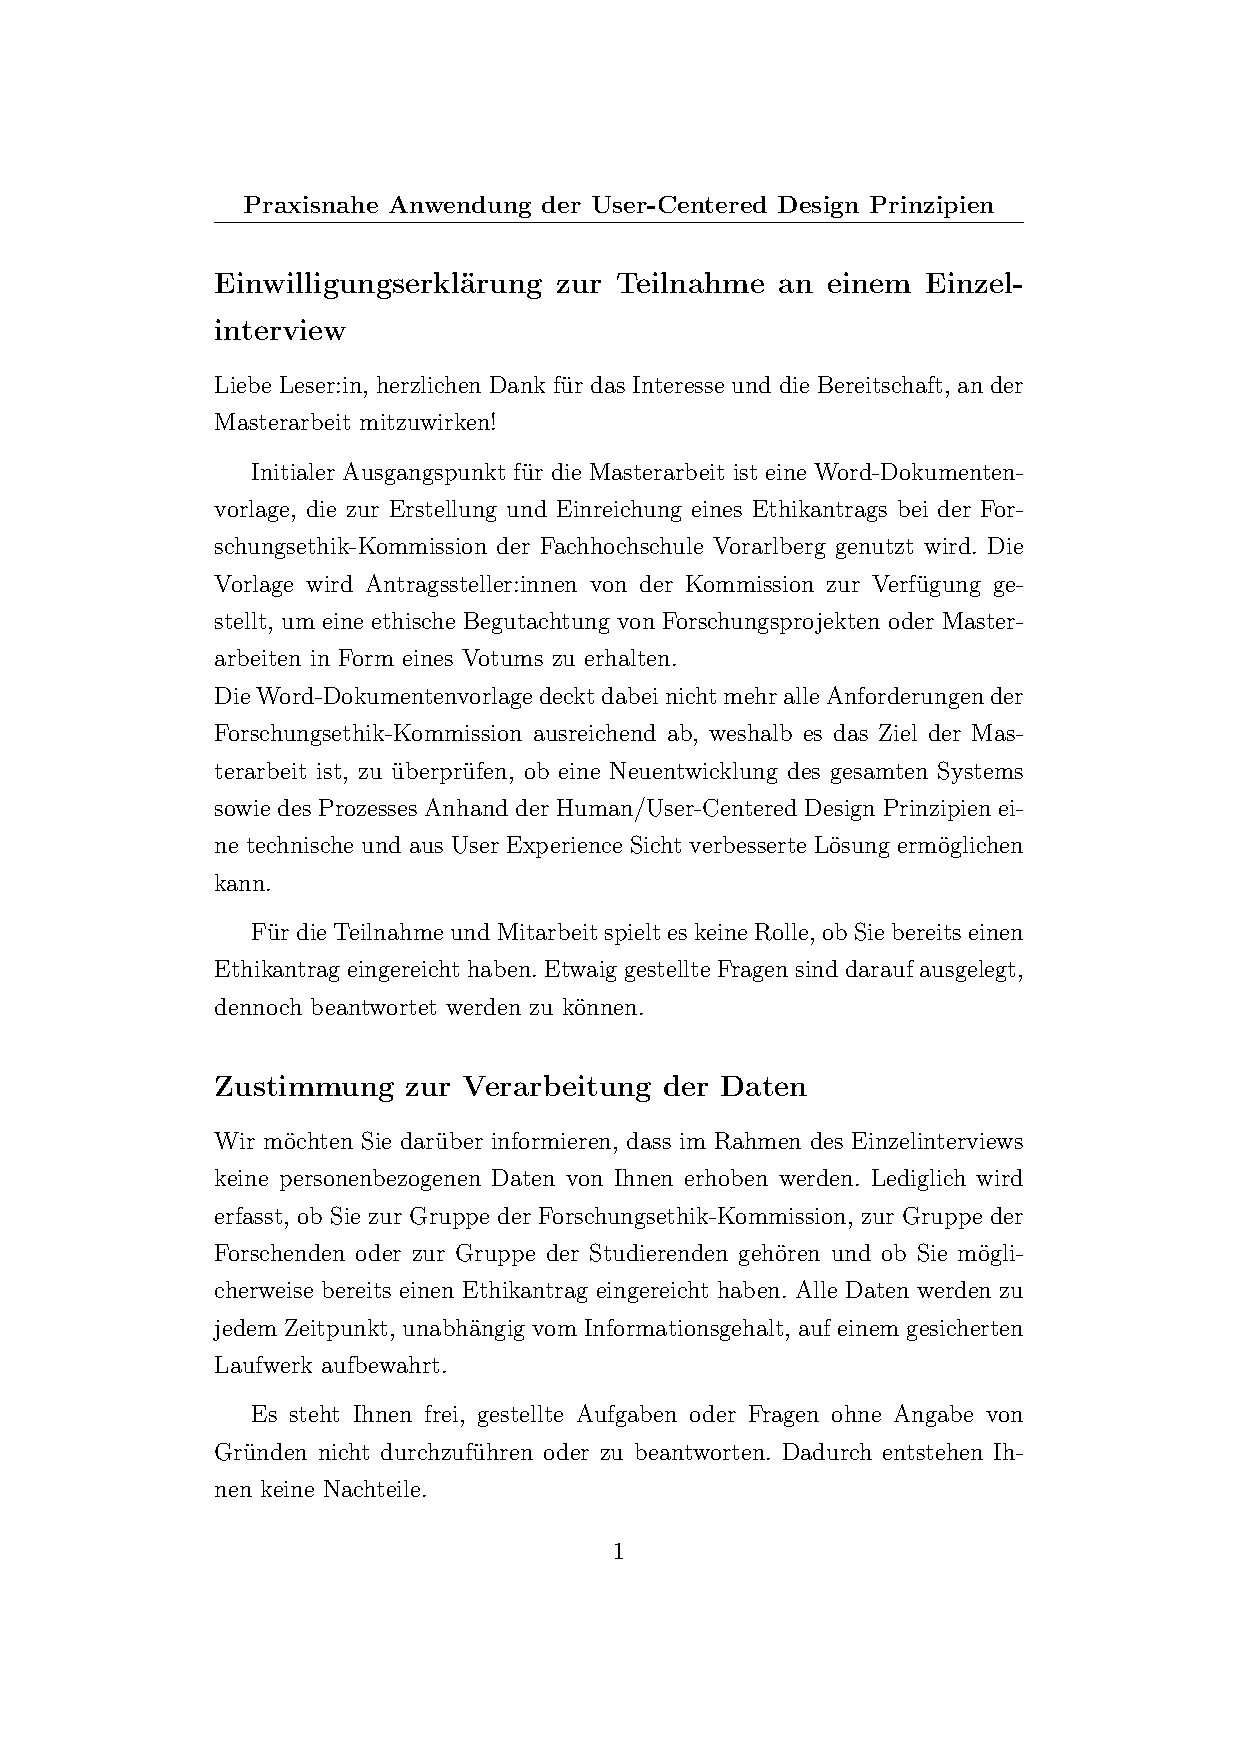
\includepdf[pages=-]{documents/Luidold_Informed-Consent_Einzelinterview.pdf}

\chapter{Einwilligungserklärung zur Teilnahme an einer Gruppendiskussion}
\label{appendix:informed-consent-gruppendiskussion}

Anhang \ref{appendix:informed-consent-gruppendiskussion} enthält die auf Basis von Anhang \ref{appendix:ursprüngliches-informed-consent-formular} ab Seite \pageref{appendix:ursprüngliches-informed-consent-formular} neu geschaffene Einwilligungserklärung für Gruppendiskussionen. Die Einwilligungserklärung wurde Anhand der Rückmeldung und des Feedbacks der \acl{fek} der \acl{fhv} (siehe Anhang \ref{appendix:rückmeldung-fek} ab Seite \pageref{appendix:rückmeldung-fek}) konkretisiert.

\subsubsection*{Durchgeführte Änderungen}
\label{appendix:änderungen-informed-consent-gruppendiskussion}

Folgende Änderungen wurden im Vergleich zur ursprünglichen Variante vorgenommen:
\begin{itemize}
    \item Der Titel des Dokumentes wurde präzisiert, sodass klar ist, dass es sich um eine Einwilligung für eine Gruppendiskussion handelt
    \item Im Abschnitt \textit{Zustimmung zur Verarbeitung der Daten} wurde präzisiert, dass die Datenerhebung im Rahmen einer Guppendiskussion stattfindet
    \item Im Abschnitt \textit{Einwilligung} wurde die Einwilligung zur Tonbandaufzeichnung explizit aufgenommen, statt mittels einer optionalen Zustimmung gehandhabt zu werden
\end{itemize}

\subsubsection*{Anmerkungen}
\label{appendix:anmerkungen-informed-consent-gruppendiskussion}

Die Einwilligungserklärung enthält im ersten Abschnitt einen Absatz, der fälschlicherweise behauptet, dass Fragen auch dann beantwortet werden können, wenn der:die Interviewpartner:in noch keinen Ethikantrag eingereicht hat. Im Zuge der Umstrukturierung der Interviews wurde der Fokus der Gruppendiskussion explizit auf die \acl{fek} der \acl{fhv} gelegt, die naturgemäß ausreichend Kenntnisse über den Prozess des Ethikantrages verfügt -- es wurde vergessen, den angesprochenen fehlerhaften Absatz zu entfernen.

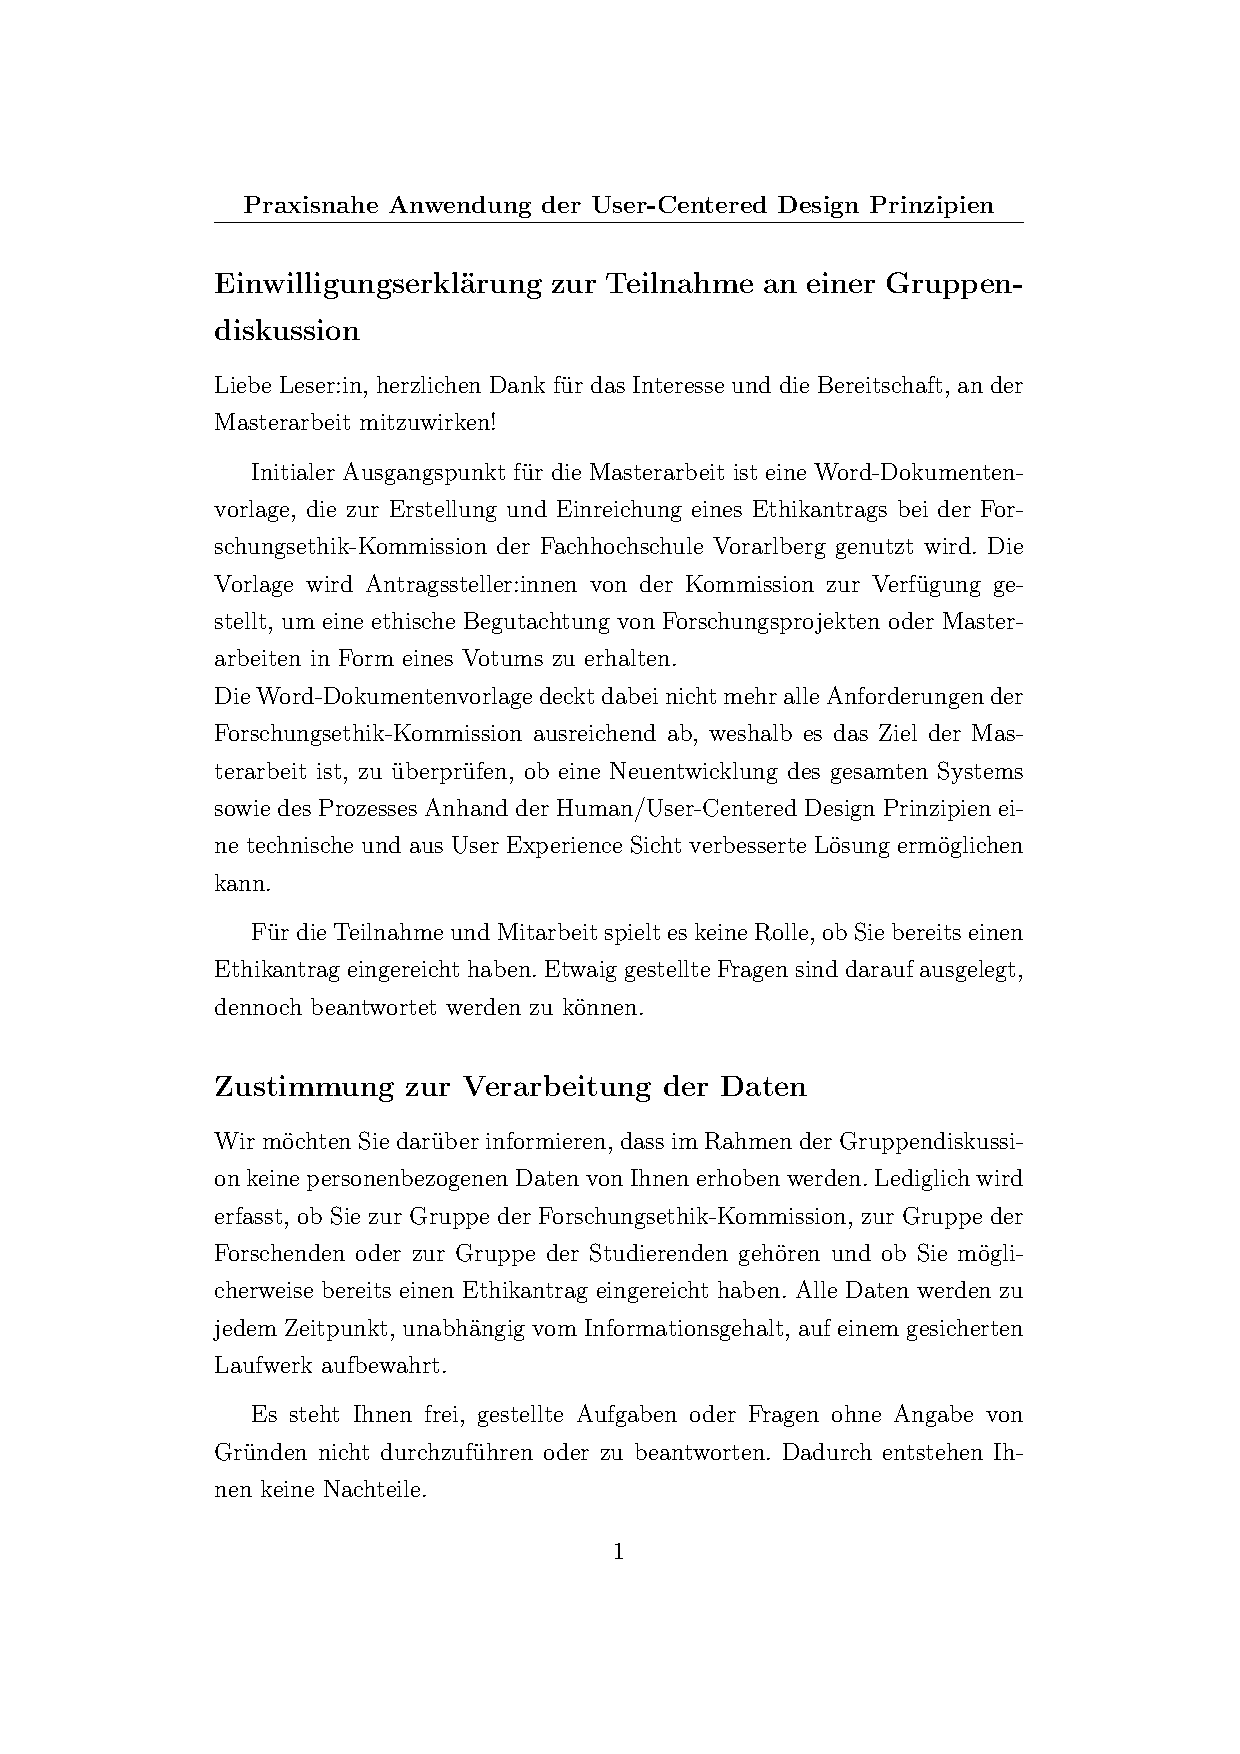
\includepdf[pages=-]{documents/Luidold_Informed-Consent_Gruppendiskussion.pdf}

\chapter{Einzelinterview \#1}
\label{appendix:interview-1}

\section{Informationen zum Interview}
\label{appendix:interview-1-infos}

Das Einzelinterview mit Interviewpartner:in A wurde am Dienstag, den 18.04.23, in den Räumlichkeiten der \ac{fhv} geführt und mittels Tonbandaufnahme aufgezeichnet. Interviewpartner:in A gehört zur Gruppe der Forschenden, die bereits einen Ethikantrag eingereicht haben.

Das Transkript des Interviews enthält beinahe 1:1 das gesprochene Wort, wobei Füllwörter wie beispielsweise \enquote{ähm} etc. der Lesbarkeit halber entfernt wurden. Zusätzlich wurden an zwei Stellen im Transkript Antworten angepasst, um den Datenschutz zu wahren -- diese sind entsprechend gekennzeichnet.

\section{Transkript}
\label{appendix:interview-1-transkript}

\textbf{Dominic:} Gut, also noch einmal auch für die Aufnahme herzlichen Dank, dass Sie sich Zeit nehmen für meine Masterarbeit und mein Interview zum Thema \enquote{Praxisnahe Anwendung der User-Centered Design Prinzipien im Rahmen der Neuentwicklung des Ethikantrag-Tools für die Ethikkommission der FH Vorarlberg}.

Jetzt würde ich direkt schon einmal ganz frech mit der ersten Frage starten, die direkt ins Thema hineingeht, und zwar: Warum haben Sie im Rahmen Ihrer Forschungsarbeit überhaupt einen Ethikantrag gestellt?

\textbf{Interviewpartner:in A:} Ja, ich denke wir hätten es eventuell nicht unbedingt machen müssen, aber es waren doch Studierende mit einbezogen, wo eventuell, ja sagen wir, Schaden entstehen hätte können, wenn jemandem schwindelig wird. Wir haben ja Augmented Reality Brillen im Unterricht eingesetzt und weil wir mit Gruppen aus der Schweiz zusammengearbeitet haben, und die Schweizer hätten auf jeden Fall einen Ethikantrag stellen müssen, haben wir als Lead gesagt, wir übernehmen das, da wir selber die Ethikkommission bei uns an der Fachhochschule haben.

\textbf{Dominic:} Okay. Und nachdem Sie den Ethikantrag jetzt gestellt haben und in dem Fall auch den Lead übernommen haben, weil es die Schweizer Kolleg:innen eh gebraucht hätten, können Sie mir einmal den grundlegenden Prozess aus Ihrer Sicht als Antragsteller:in beschreiben, wie denn so ein Ethikantrag abläuft? Von der Erstellung hin bis zur Einreichung einfach die ganzen Schritte, die Sie da vielleicht noch im Kopf haben.

\textbf{Interviewpartner:in A:} Ja, das war jetzt schon wieder relativ lange her. Also ich denke, dass ich Kontakt aufgenommen habe mit \textit{der Ethikkommission}\footnote{Im Interview wurde an dieser Stelle ein konkreter Name genannt. Im Sinne des Datenschutzes findet sich hier eine sinngemäße Verallgemeinerung wieder.} und das ist ja dann das Prozedere, das beschrieben ist, dass es klare Vorgaben gibt. Die habe ich dann alle eingereicht, was notwendig war, und das, was noch gefehlt hat, habe ich in diesem Zeitraum noch nachgereicht. Dann gab es ein Feedback, ein Votum von der Ethikkommission und das habe ich beziehungsweise haben wir dann als Gruppe, ich habe das ja nicht alleine gemacht, mit eingearbeitet und die Studierenden informiert und das alles aufeinander abgestimmt. Das, was wir überarbeitet haben, die Änderungen haben wir dann tatsächlich der Ethikkommission noch einmal vorgelegt, sodass sie sehen, dass das, was sie verlangt haben, wir dann auch wirklich geändert haben.

\textbf{Dominic:} Wenn ich das so richtig mitbekommen habe, dann würden Sie sagen, dass der Prozess grundlegend eigentlich schon relativ verständlich ist, wie er momentan abläuft?

\textbf{Interviewpartner:in A:} Grundlegend ist es für mich verständlich gewesen. Es ist natürlich ein Aufwand, aber ich fand es für mich schon klar strukturiert. Ich wusste schon, was ich zu machen hatte und ich denke, dass es schon auch gerechtfertigt ist von der Ethikkommission einen gewissen Level oder Standard einzuhalten, den man auch erbringen muss, denn es ist ja auch ein Gütesiegel, das sie vergeben. Ich weiß nicht mehr, ob mir im Einzelnen etwas unklar war, aber wenn habe ich mich an \textit{die Ethikkommission}\footnote{Im Interview wurde an dieser Stelle ein konkreter Name genannt. Im Sinne des Datenschutzes findet sich hier eine sinngemäße Verallgemeinerung wieder.} gewandt und nachgefragt. Aber es ist schon klar beschrieben.

\textbf{Dominic:} Und gerade eine Frage dazu: In dem Fall, nachdem der Prozess für Sie nicht unbedingt unverständlich war, würden Sie trotzdem vielleicht Punkte daran ändern oder sagen Sie der Prozess an sich ist soweit eigentlich klar oder in sich schlüssig oder sehen Sie da, als jemand der wirklich einen Antrag gestellt hat, aus der Perspektive als Antragsteller:in Punkte, die Sie einfach noch einmal anders handhaben würden, wenn Sie persönlich in der Forschungsethik-Kommission wären?

\textbf{Interviewpartner:in A:} Puh. Das weiß ich jetzt eigentlich auch nicht mehr. Ich denke, ich glaube es ist alles in Papierform gelaufen beziehungsweise Dateien hin und her geschickt. Vielleicht wäre das eine Vereinfachung, wenn man das alles in digitaler Form einreichen kann, dass das nicht per E-Mail hin und her geschickt werden muss. Das wäre vielleicht eine Möglichkeit, wie man den Prozess vereinfachen könnte.

\textbf{Dominic:} Dann würden Sie einfach klar sagen, das Hin- und Herschicken der Word-Antragsvorlage die es gibt, dass das in einer digitaleren Form, wenn das vorhanden wäre, das würde helfen.

\textbf{Interviewpartner:in A:} Ja, genau.

\textbf{Dominic:} Nachdem Sie jetzt gerade den Prozess beschrieben haben, würden Sie wieder einen Ethikantrag stellen, wenn es Projekte gibt, bei denen es die Umstände zulassen?

\textbf{Interviewpartner:in A:} Ja, klar. Ich denke, dass das eine feste Institution oder feste Größe ist und Gott sei Dank haben wir das in der Zwischenzeit. Und da wir jetzt im Studiengang und im Forschungszentrum immer entweder mit Studierenden oder Patient:innen, Bewohner:innen, Menschen und Angehörigen zu tun haben, denke ich, wird das auch in der Zukunft vermutlich noch mehr gefragt und dass das einfach auch Zeit, Stunden und Geld ist, das man mit einkalkulieren muss und das schon machen wird. Also ich möchte nicht per se sagen, wir lassen das. Ich frage das ja auch bei Studierenden, die dementsprechende Bachelor- oder Masterarbeiten machen, an, ob sie da ein Votum von der Ethikkommission brauchen, wenn dementsprechend Gruppen mit involviert sind.

\textbf{Dominic:} Gibt es vielleicht dennoch Gründe, warum Forschende sich hier an der FH nicht dazu entscheiden einen Ethikantrag zu stellen? Oder vielleicht gerade auch weil Sie die Studierenden erwähnt haben, gibt es dort vielleicht irgendwelche Gründe, abgesehen vom vielleicht Zeitaufwand oder ist es vielleicht sogar der Zeitaufwand?

\textbf{Interviewpartner:in A:} Ja, also Gründe vielleicht dass es im Forschungsdesign nicht zwingend verlangt wird, und wenn es nicht zwingend verlangt wird, dann machts niemand und wenn es nicht verlangt ist, dass viele vielleicht denken: \enquote{Ja, das ist überhaupt nicht notwendig. Ich mache nichts, was ethisch kritisch sein könnte. Ich werde niemandem Schaden zufügen, es hat jeder die Möglichkeit entweder in die Gruppe oder die Gruppe zu kommen oder davon zu profitieren.} Im Endeffekt dass dieses Verständnis, das könnte ich mir vostellen, nicht in allen Fachbereichen, in allen Disziplinen ausreichend vorhanden ist und dass das mehr und mehr auch in der Lehre thematisiert und sensibilisiert werden sollte. Oder wie kürzlich die \textit{forward}\footnote{Anmerkung: Event-Format der Fachhochschule Vorarlberg (\url{https://www.fhv.at/forward-event/})} stattgefunden hat, dass das einfach schon ein Thema ist und auch sensibilisiert wird dafür.

\textbf{Dominic:} Also würden Sie konkret zusammenfassen, dass es mehr externe Faktoren sind als die Arbeit oder der Prozess der Ethikkommission selbst?

\textbf{Interviewpartner:in A:} Würde ich schon sagen. Es hat auch etwas mit der Haltung des Einzelnen zu tun. Und wenn es den Prozess selber erleichtern würde, oder wie der Prozess ist, ob der aufwendig ist, schwierig, das merkt jemand, ein Antragsteller, erst dann, wenn er es tatsächlich macht und er hat dann ja nicht unbedingt einen Vergleich damit oder tatsächlich mit den Auflagen oder dem Votum, das dann die Ethikkommission abgibt. Ich würde so spontan sagen, dass wenn jemand einen Antrag stellt, dass es dann gut ist, dass das Prozedere, der Ablauf und alles, was es zu machen gibt, so einfach wie möglich ist und dass man das mit allen möglichen Designs und Technologien, und auch mit dem, was Sie vielleicht beabsichtigen, verbessern könnte, ja? Aber dass das letztendlich, diese Perfektion und von dem, was man verändert, glaube ich nicht unbedingt etwas daran ändert, ob mehr oder weniger Anträge gestellt werden. Ich glaube jetzt auch nicht, dass das der Eine oder der Andere Ethikkommission A und B, die an anderen Hochschulen oder Universitäten oder irgendwo anders sind, dass man die vergleicht. Ich kenne es von Deutschland her, dass man vielleicht schaut: wo ist es am einfachsten, wo ist der Aufwand gering oder wie viel kostet es, wie schnell geht es, dass ich irgendwo meinen Antrag durchbekomme. Teilweise kostet es ja auch wirklich Geld, das wissen wir vielleicht, oder viele, gar nicht zu schätzen, dass das aktuell oder gar nie irgendetwas kostet hier an der Fachhochschule. Aber es gibt schon auch Ethikkommissionen, wo man wirklich auch Geld zahlen muss, das dann auch im Budget vom Forschungsprojekt mit vorgesehen ist.

\textbf{Dominic:} Sie haben ganz zu Beginn des Interviews schon die Dokumente, die per E-Mail hin und her geschickt werden, angesprochen, die nicht unbedingt optimal sind, wenn man das so sagen kann. Es ist eine Antragsvorlage, die natürlich mit Microsoft Word kompatibel ist und natürlich auch mit den anderen, größeren freien Texteditoren. Was waren dort vielleicht Ihre konkreten Erfahrungen mit der Antragsvorlage? Haben Sie das noch im Kopf?

\textbf{Interviewpartner:in A:} Also, ich muss sagen, nicht wirklich.

\textbf{Dominic:} Gibt’s in dem Fall nichts, das Sie, nachdem der Antrag schon länger her ist..

\textbf{Interviewpartner:in A:} .. wo ich jetzt sagen könnte, das und das.

\textbf{Dominic:} Genau. Ob Ihnen vielleicht noch etwas im Kopf geblieben ist, was ist positiv aufgefallen oder eher negativ.

\textbf{Interviewpartner:in A:} Im Normalfall kann ich mich schon daran erinnern, wenn irgendein Dokument, an dem ich gearbeitet habe, wenn ich das mit dem Mac verwende, irgendwie nicht zu benutzen ist oder nicht funktioniert, wenn es zu bearbeiten ist, wenn wir es innerhalb der Gruppe wieder hin und her schicken. Nein, also mir fällt nichts ein.

\textbf{Dominic:} Das finde ich ganz interessant eigentlich, weil gerade, wenn einem etwas konkret einfällt und so spontan, dann muss es stark aufgefallen sein.

\textbf{Interviewpartner:in A:} Ja, genau, ja.

\textbf{Dominic:} Vielleicht jetzt noch die letzte Frage, das Interview ist tatsächlich gar nicht so lange. Nachdem Sie jetzt wissen, dass ich mich mit meiner Masterarbeit mit dem ganzen Thema beschäftige, was die Anforderungen sind, was die Wünsche sind, sowohl aus Sicht der Kommission als auch aus Sicht der Antragsteller:innen. Sie haben es eh schon erwähnt, die Word-Dokumente, die Sie herunterladen und per E-Mail verschicken sind nicht ganz optimal. Gibt es irgendetwas, dass Sie sich ganz konkret wünschen würden, wo Sie sagen, wenn Sie wieder einen Ethikantrag ausfüllen, dann würde Ihnen das das Ganze noch einmal erleichtern oder vielleicht auch Hilfestellungen, die Sie sich während dem Ausfüllen gewünscht hätten oder Beispiele oder irgendetwas in die Richtung?

\textbf{Interviewpartner:in A:} Ich weiß jetzt nicht, ob das hier passt, aber dass es vielleicht auch Textbausteine gibt. Nein, das wird nicht funktionieren. Meistens wird es ja beantwortet aus meinem Forschungsdesign heraus. Also nicht wirklich etwas. Es ist schon etwas her.

\textbf{Dominic:} Das ist vollkommen in Ordnung. Vielleicht hätten Sie gesagt, es soll ein Online-Formular sein, dass das Ganze ablöst und vereinfacht, oder bei der Word-Antragsvorlage bleiben, weil man dort die meisten Freiheiten hat, aber bei einer Antragsvorlage die weniger strikt ist wie die aktuelle Word-Antragsvorlage. Aber wenn Sie keine konkreten Wünsche haben, dann passt das eh ganz gut. 

Soweit ich das sehen kann, waren das schon meine Fragen, ganz kurz und bündig. Dann möchte ich mich für das Interview bedanken und wünsche Ihnen noch einen schönen Tag und eine schöne Mittagszeit.

\textbf{Interviewpartner:in A:} Danke.

\chapter{Einzelinterview \#2}
\label{appendix:interview-2}

\section{Informationen zum Interview}
\label{appendix:interview-2-infos}

Das Einzelinterview mit Interviewpartner:in B wurde am Mittwoch, den 19.04.23, in den Räumlichkeiten der \ac{fhv} geführt und mittels Tonbandaufnahme aufgezeichnet. Interviewpartner:in B gehört zur Gruppe der Forschenden, die bereits einen Ethikantrag eingereicht haben.

Das Transkript des Interviews enthält beinahe 1:1 das gesprochene Wort, wobei Füllwörter wie beispielsweise \enquote{ähm} etc. der Lesbarkeit halber entfernt wurden. Zusätzlich wurden an zwei Stellen im Transkript Antworten angepasst, um den Datenschutz zu wahren -- diese sind entsprechend gekennzeichnet.

\section{Transkript}
\label{appendix:interview-2-transkript}

\textbf{Dominic:} Okay, die Aufnahme läuft. Vielen Dank für die Bereitschaft beim Interview für meine Masterarbeit mit dem vorläufigen Arbeitstitel \enquote{Praxisnahe Anwendung der User-Centered Design Prinzipien am Beispiel der Neuentwicklung des Ethikantrag-Tools der Fachhochschule Vorarlberg} mitzuwirken.

Ich würde jetzt direkt einfach mit der ersten Frage ganz frech schon starten: Warum hast du denn einen Ethikantrag gestellt?

\textbf{Interviewpartner:in B:} Weil wir Forschung mit Menschen machen und es da eben wichtig ist, zu berücksichtigen, ob da Risiken auftreten und was das eben für Folgen haben könnten.

\textbf{Dominic:} In dem Fall für dich ganz klar gewesen oder für euch im Forschungsprojekt, dass da ein Ethikantrag wirklich notwendig ist?

\textbf{Interviewpartner:in B:} Ja, gerade wenn es um Menschen geht. Es ist natürlich immer etwas schwierig, ab wann braucht man sowas, braucht man für einen normalen Usability-Test einen Ethikantrag? Also da sind die Grenzen schon noch etwas schwammig und da wär eine Unterstützung von einem Tool sicher hilfreich das zu entscheiden, ob es überhaupt einen Ethikantrag braucht.

\textbf{Dominic:} Okay. Dann würde ich direkt mit der nächsten Frage weitermachen, und zwar: Nachdem jetzt eigentlich relativ klar war, dass ein Ethikantrag gestellt werden muss, weil eben Menschen involviert sind, würde mich interessieren, wie denn die Schritte aus Sicht eines:einer Antragsteller:in, also aus deiner Sicht, aussehen, die man durchläuft, wenn man Ethikantrag einreicht? Wie da der Prozess so ist?

\textbf{Interviewpartner:in B:} Also konkret in meinem Fall war es so, man lädt sich den Antrag runter, liest den durch, stellt fest, dass man da allerhand anderer Dinge noch vorbereiten muss damit man den Antrag ausfüllen kann und ja, bearbeitet nach und nach die Punkte, die dafür notwendig sind. Was ganz wichtig ist, ist eben, dass das Forschungsdesign schon vorher ziemlich detailliert ausgearbeitet sein muss, damit man den Antrag überhaupt ausfüllen kann.

\textbf{Dominic:} Der weitere Ablauf, im Sinne was passiert wenn der Ethikantrag bei der Kommission eingereicht wurde und wie dann der Ablauf für dich als Antragsteller:in ist, das ist soweit in dem Fall auch verständlich?

\textbf{Interviewpartner:in B:} Das war relativ klar dass da dann die Ethikkommission zusammentreten muss, also zunächst begutachtet werden muss von den einzelnen Mitgliedern und dann irgendwann einmal das Feedback kommt.

\textbf{Dominic:} Nachdem wir jetzt eben kurz abgeklärt haben, warum man einen Ethikantrag stellen sollte oder warum ihr einen Ethikantrag gestellt habt und wie der Prozess so abläuft, würdest du wieder einen Ethikantrag stellen, eben mit dem Wissen, wie der gesamte Prozess abläuft?

\textbf{Interviewpartner:in B:} Ja, auf jeden Fall. Also wenn es wieder die Voraussetzungen gibt, dass mit Menschen geforscht wird und da eventuell Risiken verknüpft sind, dann ist das auf jeden Fall hilfreich da einen Antrag zu stellen. Es geht auch darum, dass man selber das Feedback bekommt, was man vielleicht verbessern sollte am Forschungsdesign, falls Risiken nicht korrekt berücksichtigt sind.

\textbf{Dominic:} Okay. Nachdem wir jetzt das kurz einmal zusammengefasst haben, gibt es konkrete Punkte, die du jetzt am Prozess vielleicht verändern würdest, einfach weil du weißt, wie der Ethikantrag aussieht, wie er auszufüllen ist, was es da für Anforderungen gibt, wie der weitere Prozess aussieht.

\textbf{Interviewpartner:in B:} Ja, ich würde es begrüßen wenn, man kein Word-Formular mehr ausfüllen muss, sondern dass man da ein bisschen durchgeleitet wird durch den Prozess. Also es sind auch einige Dinge die einem so vorkommen zumindest, dass sie doppelt ausgefüllt werden müssen, je nachdem, ob es ein Produkt wird oder ob es nur eine Forschung ist, dass man da unterschiedliche Blätter ausfüllen muss.

\textbf{Dominic:} Was die Antragsvorlage abfragt, wiederholt sich dann in diesem Fall stellenweise aus deiner Sicht?

\textbf{Interviewpartner:in B:} Genau. Also je nachdem, ob es ein Produkt ist oder eine Forschung muss man unterschiedliche Dinge ausfüllen, die aber meistens schon davor einmal erwähnt wurden.

\textbf{Dominic:} Gibt es sonst noch etwas, was dir bei der Antragsvorlage oder auch generell im Prozess aufgefallen ist oder an dem wie die Fragen gestellt werden oder was abgefragt wird, wo du etwas abändern würdest?

\textbf{Interviewpartner:in B:} Ja, also eh schon kurz angesprochen. Die erste Entscheidung ist: Muss ich überhaupt einen Ethikantrag stellen? Da wäre es cool, wenn es irgendein Hilfsmittel gibt, das abzuschätzen. Es ist schon klar, dass es im Endeffekt immer von der Kommission vielleicht entschieden werden muss. Je nachdem, in Grenzfällen, aber es gibt vorgelagert sicher Möglichkeiten wo man das abfangen kann, wenn ich technische Messungen irgendwo durchführe wo keine Menschen involviert sind, dann kann es zwar zur Technikfolgeabschätzung vielleicht sinnvoll seinen einen zu stellen, aber jetzt nicht unbedingt unmittelbar weil Menschen gefährdet sind.

\textbf{Dominic:} Da wir eigentlich den ganzen Prozess schon relativ gut angesprochen haben, auch was du konkret jetzt in deinem Fall verbessern würdest was dir aufgefallen ist, gibt es vielleicht Anlässe, die dir aufgefallen sind oder dir einfallen könnten, die Forschende aktiv davon abhalten, einen Ethikantrag zu stellen, obwohl diese vielleicht auch wirklich einen Ethikantrag in Betracht gezogen haben?

\textbf{Interviewpartner:in B:} Das erste ist vielleicht, dass sie nicht wussten, dass es überhaupt eine Ethikkommission gibt an der FH. Das heißt, alleine dafür wäre schon so ein Tool sinnvoll, das man verbreiten kann. Das könnte dann zum Beispiel in den Bachelor- und Masterseminaren angesprochen werden, dass man da draufgeht um einen Check zu machen, brauch ich überhaupt einen Ethikantrag oder nicht, um da eben die Awareness zu schaffen, dass es so etwas überhaupt gibt. Ich weiß nicht, ob das sowieso stattfindet.

\textbf{Dominic:} Das wäre sicherlich sinnvoll, ja.

\textbf{Interviewpartner:in B:} Vom Prozess selber, wenn man entschieden hat, man will einen Ethikantrag stellen, momentan muss man eben das Word-Formular ausfüllen, das es einem teilweise schwer macht. Ich weiß allerdings nicht ob das ein Mac-spezfisiches Problem ist, aber zum Beispiel will ich etwas hineinschreiben und dann springt der Cursor gleich zum nächsten Feld, ich kann da gar nichts hineinschreiben, wenn ich nicht ganz genau an den Start klicke. Solche Sachen.

\textbf{Dominic:} Also wirklich nicht nur von der Fragestellung her sondern rein von der Bedienung schon.

\textbf{Interviewpartner:in B:} Rein von der Bedienung, aber ich denke das ist in der neuesten Version behoben. Aber das ist ja nur ein Teil, das heißt man bekommt ja darauffolgend, also man reicht den ein und wartet bis man Feedback bekommt. Da wäre es interessant, wenn es so eine Prozessansicht geben würde, wo man sieht, wo steckt der Antrag gerade, er ist jetzt in Begutachtung, die Kommission muss zusammentreffen und das nächste Treffen findet dann und dann statt.

\textbf{Dominic:} Also dass man ein bisschen abschätzen kann, wo steht man mit seinem Forschungsprojekt mit dem Antrag.

\textbf{Interviewpartner:in B:} Genau, das läuft momentan noch per E-Mail, teilweise zumindest, dass man da dann direkt in dem Portal zum Beispiel einen Überblick hätte. Da gibts ja, wenn man das Feedback bekommt, das Feedback auch wieder per Mail und da ist die Frage, ob es dann so ein Vor und Zurück geben soll, also dass man dann Verbesserungen einreichen kann, ob das überhaupt gewünscht ist von der Ethikkommission. Das wäre vielleicht auch noch so eine Frage. Dass die dann noch einmal darüber gehen und sagen das passt oder ob das eh schon damit abgehandelt ist wenn sie den Vorschlag kommuniziert haben, dass das dann, unter der Voraussetzung, dass das umgesetzt wird, genehmigt ist.

\textbf{Dominic:} Man könnte es ein bisschen so zusammenfassen mit: Ab dem Zeitpunkt wo der Antrag eingereicht wurde bis man die Rückmeldung bekommt ist es bisschen wie eine Blackbox. Man weiß jetzt genau was passiert.

\textbf{Interviewpartner:in B:} Jain. Man bekommt schon das Feedback, die Ethikkommission trifft dann und dann das nächste Mal zusammen und wird es dann begutachten aber das ist dann in einem Mail unter vielen tausenden. Wenn das wirklich so eine Art Portal wäre wo man dann reinschauen kann, das sind die Anträge die ich gestellt habe, da gab es die und die Auflage, die und die Auflage habe ich nachträglich noch einmal eingereicht zum Check und es wurde dann akzeptiert.

\textbf{Dominic:} Im Endeffekt also auch eine Historie, was man früher schon eingereicht hat vielleicht. Das man auch darauf Bezug nehmen kann, wenn man wieder etwas sucht.

\textbf{Interviewpartner:in B:} Genau. Oder wenn ich zum Beispiel sehe, ich hab beim vorherigen Antrag das und das Feedback bekommen, nochmals als Reminder was muss ich dann dieses Mal gleich von vornherein berücksichtigen, wenn ich einen neuen Antrag stelle.

\textbf{Dominic:} Gibt es sonst noch irgendwelche konkreten Ideen oder Vorschläge oder auch wirklich Kritik, die man in einem neuen System umsetzen könnte oder besser machen könnte, die wir jetzt noch nicht angesprochen haben? Irgendetwas, dass dir konkret vielleicht einfällt?

\textbf{Interviewpartner:in B:} Ja, die Ideen die gehen dann eher weiter, aber das ist dann eher für die Ethikkommission relevant, dass es für die vielleicht auch hilfreich wäre. Momentan wird der Ethikantrag wahrscheinlich per Mail weitergereicht, das wirst du wahrscheinlich eh erheben wie das dort läuft, und dann müssen die einzelnen Evaluatoren das durchlesen, sich anschauen, Kommentare dazu machen. Das heißt, es entstehen dann unterschiedlich viele Dokumente mit Kommentaren darin, die wieder zusammengeführt werden. Ob es da eine Möglichkeit gibt, diesen Prozess zu vereinfachen, dass da nicht zehn verschieden Versionen vom Antrag mit Kommentaren da sind, sondern dass das vielleicht gesammelt schon angemerkt werden kann. Da ist vielleicht, wie auch bei der heuristischen Inspektion, zum Beispiel, so dass man es zuerst für sich betrachtet anschaut, jeder das Feedback dazu gibt und erst danach dieses Feedback dann besprochen wird in der großen Runde. Dass es da einen Support gibt, aber wie gesagt, das kann ich jetzt nicht einschätzen, weil ich nicht in der Kommission bin.

\textbf{Dominic:} Das werde ich auf jeden Fall auch mal so in der Kommission, in die Runde, die Frage stellen, wie der Prozess da eigentlich abläuft, um da wirklich auch das Feedback zu erhalten.

\textbf{Interviewpartner:in B:} Und auch die Frage, wer kann denn überhaupt einen Antrag bearbeiten, gibt es da vielleicht ein Zuweisungssytem, wer bekommt diesen Antrag zur Begutachtung.

\textbf{Dominic:} Ist das aus Sicht von Antragsteller:innen auch interessant, weil meistens arbeitet man ja in einem Team, wenn es um ein Forschungsprojekt geht. Wie war es bei euch, war da wirklich nur eine Person damit beschäftigt?

\textbf{Interviewpartner:in B:} Bei uns ist es so, wenn wir vom \textit{Forschungszentrum}\footnote{Im Interview wurde an dieser Stelle ein konkreter Name genannt. Im Sinne des Datenschutzes findet sich hier eine sinngemäße Verallgemeinerung wieder.} einen Antrag stellen, dann dürfen natürlich nicht die \textit{Forschungszentrum}\footnote{Im Interview wurde an dieser Stelle ein konkreter Name genannt. Im Sinne des Datenschutzes findet sich hier eine sinngemäße Verallgemeinerung wieder.}-Mitglieder die in der Kommission sind darüber befinden, ob das durchgeht oder nicht. Also da gibt es die Ausschlussgründe, wenn man befangen ist.

\textbf{Dominic:} Die Frage war eher in die Richtung gedacht, beispielsweise wenn jetzt du in einem Forschungsprojekt tätig bist, dann füllst du den Ethikantrag aus im Online-Portal. Schauen dann noch andere Team-Mitglieder des Forschungsprojektes darüber?

\textbf{Interviewpartner:in B:} Genau, das wäre noch eine andere Funktion, dass man da kollaborativ daran arbeiten kann. Also dass ich den ersten Teil ausfülle, eine Kolleg:in füllt dann diese Zielsetzung zur Forschung aus, je nach dem gibt es ja auch unterschiedliche Möglichkeiten.

\textbf{Dominic:} Okay, also dass es nicht nur eine Person im Endeffekt ausfüllt, sondern dass mehrere Personen darauf Zugriff haben wäre auch vorteilhaft zu einer Word-Antragsvorlage.

\textbf{Interviewpartner:in B:} Genau. Es wird dann wahrscheinlich schon einen Verantwortlichen geben, der das dann einreicht und darüber schaut über alles, aber ja, die Idee wäre mir vorher noch gar nicht gekommen. Wenn ich zurück denke, dann war es eigentlich auch so, dass wir den Antrag hin und her geschickt haben als Word-Dokument und dann Ergänzungen gemacht haben.

\textbf{Dominic:} Ich glaube, wir haben jetzt konkret eh alle meine grundsätzlichen Fragen abgehandelt. Das Interview ist eh relativ kurz angelegt mit gut 15-20 Minuten, um einen ersten Input zu bekommen. Hast du sonst noch irgendetwas, was dir in der Vorbereitung auf das Interview eingefallen ist bei der Durchsicht des Ethikantrages oder auch sonst irgendetwas?

\textbf{Interviewpartner:in B:} Nein, von daher nichts Weiteres. Wie gesagt, mein Hauptkritikpunkt ist das Word-Formular und dass es eben sehr schwierig ist, die Übersicht zu bewahren. Gerade, wenn mehrere Leute daran arbeiten, wie die schlussendliche Version zustande gekommen ist. Das wäre vielleicht auch so eine Idee, dass man da mittracken kann, wer was hinzu geschrieben hat und von wem welcher Input gekommen ist.

\textbf{Dominic:} Alles klar. Dann bedanke ich mich für das Interview.

\textbf{Interviewpartner:in B:} Gerne.

\chapter{Gruppendiskussion mit der \acl{fek}}
\label{appendix:gruppendiskussion}

\section{Informationen zur Gruppendiskussion}
\label{appendix:gruppendiskussion-infos}

Die Gruppendiskussion mit Interviewpartner:in C, D, E und F wurde am Mittwoch, den 19.04.23, in den Räumlichkeiten der \ac{fhv} geführt und mittels Tonbandaufnahme aufgezeichnet. Die genannten Interviewpartner:innen gehören der Gruppe der \acl{fek} an.

Das Transkript des Interviews enthält beinahe 1:1 das gesprochene Wort, wobei Füllwörter wie beispielsweise \enquote{ähm} etc. der Lesbarkeit halber entfernt wurden. Zusätzlich wurden an mehreren Stellen im Transkript Antworten angepasst, um den Datenschutz zu wahren -- diese sind entsprechend gekennzeichnet.

\section{Transkript}
\label{appendix:gruppendiskussion-transkript}

\textbf{Dominic:} Okay, dann möchte ich jetzt auch für die Aufnahme herzlich danken, dass ihr euch heute Zeit nehmt bei meinem Interview mit dabei zu sein für meine Masterarbeit \enquote{Praxisnahe Anwendung der User-Centered Design Prinzipien mit dem Fokus der Neuentwicklung des Ethikantrag-Tools der Forschungsethik-Kommission der Fachhochschule Vorarlberg}. Ich hätte jetzt einfach gesagt, ich fange direkt mit den Fragen an und wir schauen einfach, wie weiter wir kommen oder wo uns das Ganze hinführt. Gerne jederzeit unterbrechen.

\textbf{Interviewpartner:in C:} Sollen wir nicht sagen, wer alles anwesend ist? In sechs Monaten weiß niemand mehr, wer da war.

\textbf{Dominic:} Ich weiß es ja, da ich das Interview transkribiere und im Protokoll ist es nicht mehr vorhanden, wer wer ist.

\textbf{Interviewpartner:in C:} Okay.

\textbf{Dominic:} Meine erste Fragen an euch wäre eigentlich, warum sollten Forschende an der FH einen Ethikantrag stellen?

\textbf{Interviewpartner:in C:} Wann immer solche Fragen kommen, gehen wir einfach rundherum. Dann haben wir das zügiger erledigt, oder? Dann muss auch keiner das Gefühl haben er sagt jetzt nichts, weil jemand anderes etwas Gescheiteres sagt.

\textbf{Interviewpartner:in D:} Mhm, mhm. Es gibt zwei Motivationen für einen Ethikantrag, die intrinsische und die extrinsische. Die intrinsische ist einfach um auch die Qualität des Vorhabens von anderen betrachten und bewerten zu lassen und sich überhaupt, sag ich mal, damit auseinanderzusetzen, welche ethischen Implikationen die eigne Forschung eigentlich haben kann. Ich glaube, dass das im normalen Prozess untergeht. Man versucht hoffentlich methodisch sauber zu arbeiten, aber, ja, diese ethischen Betrachtungen und ethischen Kriterien sind nicht im Fokus. Damit hat man noch einmal die Gelegenheit, mehr Qualität in die eigene Forschung zu bekommen. Rückmeldung aus verschiedenen Perspektiven von Menschen mit Erfahrung im Bereich der Forschung und das ist eine sinnvolle Institution.

\textbf{Interviewpartner:in E:} Eigentlich hast du alles gesagt.

\textbf{Interviewpartner:in D:} Oh.

\textbf{Interviewpartner:in E:} Extrinsich, Journal-Artikel und so weiter, wo man es einfach braucht für den Verwertungsprozess. Intrinsisch, Feedback. Ich glaube, es ist auch gut wenn man es vielleicht zielgruppenspezifisch anspricht. Bei Forschenden gehört es einfach zum Prozess. Da ist, glaube ich, eine Aufgabe, dass wir die Awareness schaffen, dass es auch nicht wehtut, wenn man sich noch einmal von Kolleg:innen übers Design drüberschauen lässt und nicht für sich in Anspruch nimmt, eh schon alles zu wissen. Bei Studierenden wie zum Beispiel dir ist es eine Erfahrung, einen Einblick darin zu kriegen, wie so ein Prozess abläuft. Da geht es dann gar nicht so sehr noch ums Feedback. Doch, vielleicht auch wenn man die Zeit hat, es dann auch umzusetzen, das ist dann wahrscheinlich die Limitation. Aber auch einfach, um den Prozess etwas kennenzulernen.

\textbf{Interviewpartner:in C:} Es ist vieles gesagt worden. Ich glaube, es ist auch ein Qualitätsmodell das wir da durchziehen. Für die Studierenden ist es eine gute Erfahrung, viel zu oft lässt man dieses Thema Ethik aus der Hype-Diskussion einfach draußen. Es ist eine gute Lehre für die Lehrenden aber auch die Studenten. Eigensicht, Fremd- und Außenansicht ist eh gesagt worden.

\textbf{Interviewpartner:in F:} Korrektivfunktion haben wir gehabt. Ich kann auch nichts Neues dazu beitragen.

\textbf{Dominic:} Wenn wir gerade bei den Gründen bleiben, warum man einen Ethikantrag stellen sollte, gibt es aus eurer Sicht Anlässe, die Forschende davon abhalten einen Ethikantrag zu stellen, obwohl sie sich vielleicht dafür interessieren würden?

\textbf{Interviewpartner:in D:} Der Faktor Zeit ist ein ganz entscheidender. Vieles wird mit heißer Nadel gestrickt in der Forschung. Ja, ich würde jetzt einmal sagen es liegt nicht an den Persönlichkeiten in der Forschung, ich glaube die sind schon sehr gut strukturiert, haben ein gutes Projektmanagement. Sonst wären sie wahrscheinlich nicht in dieser Funktion tätig. Von daher würde ich einfach einmal behaupten, es ist schon ein bisschen dem Kontext geschuldet, dass man auf Calls kurzfristig draufspringt, angefragt wird von Partnern aus verschiedenen Netzwerken. Dann wird das Proposal, dieser Forschungsantrag ausformuliert und es bleibt im Vorfeld nicht die Zeit, auch noch den Ethikantrag sauber mit abzugeben. Könnte ich mir vorstellen, dass das einer der Punkte ist, die einen davon abhalten. Außer natürlich es ist explizit gefordert, das gibt es immer mehr, dass Geldgeber sagen es muss ein Ethikvotum vorliegen, sonst bekommt ihr unseren Zuschlag nicht. Aber Zeit kann einen davon abhalten und vielleicht sogar auch Fachhochschulen, im Gegensatz zu Universitäten, finanzieren sich bei der Forschung ausschließlich über Drittmittel. Also wir haben keine Gelder für Forschung vom Land oder vom Bund, das ist auch ein großes Kampfthema für die Fachhochschulen. Ich glaube, wenn man in einer Führungsrolle an einer Fachhochschule ist im Bereich Forschung, will man auch, dass das Team erhalten bleiben kann, Verträge verlängert werden können und dass man dann oft die Prämisse hat, wichtiger sind die Drittmittel zu haben und der Ethikaspekt leicht hinten runterfallen kann. Ganz offen gesprochen.

\textbf{Interviewpartner:in E:} Zeit und Ressourcen. Ich würde sogar noch ein bisschen weitergehen und Advocatus Diaboli zu spielen bei dieser Geschichte. Zeit und Ressourcen gebe ich dir Recht, spielt eine große Rolle. Bei uns manchmal auch Projekte, die einfach kein Ethikvotum brauchen. Da sind die externen Motivationen nicht gegeben, weil wir die Ergebnisse nicht publizieren werden, es ist eher ein Bericht für Auftraggebende quasi. Dann ist die Frage der Qualität und wenn man da auch noch weiß wie das Budget teilweise aussieht, mit dem wir arbeiten müssen und wir wissen, dass wir etwaige gut gemeinte Auflagen gar nicht umzusetzen in der Lage wären, stellt sich die Frage, ob man die Ressourcen investieren möchte diese Kreis noch zu schließen und ein Votum mit Auflagen zu haben, die evidenter Maßen nicht umzusetzen sind beispielsweise. Was bei uns glaube ich auch noch dazukommen könnte, ich habe es vorher schon kurz anklingen lassen, das ist jetzt eine Hypothese ohne Bezug zu einem konkreten Fall von dem ich wüsste, aber ich könnte mir vorstellen, eben diese diese Einstellung: \enquote{ja, ich mach das seit zwanzig Jahren, ich bin gut in dem was ich tue, da braucht man jetzt nicht auch noch die paar Leute aus anderen Fachbereichen erzählen wollen, wie ich meine Forschung zu machen habe}. Vielleicht auch die Angst vor einem negativen Votum. Etwas zu beantragen bedeutet psychologisch immer auch das Risiko abgelehnt zu werden. Wenn ich es gar nicht erst tue, ist es potenziell bequemer. Dann haben wir natürlich noch die üblichen Geschichten: sind wir ausreichend bekannt, sind die Gründe ausreichend kommuniziert. Also die Kommunikationsarbeit.

\textbf{Interviewpartner:in C:} Glaube ich auch, ja. Also bei mir wissen die Leute, trotz immer wieder Predigten von mir, vielfach nicht, dass es auch eine Ethikkommission gibt. Das Wissen um die Ethikkommission an sich, ich bestätige es in Wirklichkeit nur, die Angst davor, dass etwas herauskommt was dann noch viel mehr Arbeit bedeutet. Die Auflagen sind ja meistens nicht die low-hanging Fruits die man da bearbeiten muss. Das zweite, da gebe ich dir auch vollkommen Recht, ist die Einstellung \enquote{ist nicht gefordert, ich mache das eh ganz anständig}. Wir in der Technik haben zum Teil auch Auftraggeber, die sagen, sollen wir es einreichen, nein, ist mein Geld, das interessiert mich nicht. Warum soll ich es dann machen? Naja, es gibt schon auch ein paar positive Antworten, warum man es macht. Aber ist kein Bedarf da, im Gegenteil, der Auftraggeber sagt nein, bloß keine Zeit dafür verschwenden. Wir wollen jetzt dann bald wissen, wie das neue Produkt funktioniert. Also da kommt es durchaus vor. Ist mir da jetzt noch nie passiert, aber sehr wohl in anderen Situationen.

\textbf{Interviewpartner:in F:} Ich denke mir, es hat mit dem zu tun was \textit{Interviewpartner:in E} vorhin gesagt hat mit dieser Awareness. Ethik oder ethische Fragestellungen grundsätzlich sind Querschnittsthemen. Wir haben zwar aktuell zumindest die Lösung, man siedelt einen Antrag am Ende des Studiums an und holt sich ein Ethikvotum wenn man eine wissenschaftliche Arbeit beginnt oder in der Forschung, das gehört dort einfach noch dazu. Der Knackpunkt wäre aber, wenn es um das Bewusstsein geht, dass es grundsätzlich zu den Menschen hin gehört. Und auch nicht unbedingt nur zu den Forschenden, sondern zu uns allen als Gesellschaft. Das ist so ähnlich wie mit der Wahlbeteiligung. Wir wissen alle, dass es da ist, aber kein Mensch schert sich. Es fehlt so eine grundlegende Ausbildung. Wir agieren auch nicht mehr ethisch in dem Bereich. Das wäre für mich jetzt noch so ein weiterer Grund oder Gedanke, warum ich abgehalten werden könnte, einen Antrag zu stellen, weil es grundsätzlich da ist. Die Alternative wäre, wir bringen das von Beginn des Studiums weg an hinein, weil es eine klassische Querschnittsmaterie ist und unabhängig davon welches Fach ich in meinem Studium mache, gehört irgend eine ethische Fragestellung hinein und das geht wirklich in jedem Fach. Also auch insbesondere in der Technik oder was hier sonst noch so gelehrt wird. Das gehört vermittelt, dass Ethik eine grundsätzliche Angelegenheit unseres Tuns ist, und das haben wir nicht.

\textbf{Interviewpartner:in E:} Darf ich noch etwas ergänzen? Jetzt hast du mich drauf gebracht und das finde ich auch noch ganz gut und ganz wichtig. Es ist glaube ich diese Unterscheidung, darüber hatten wir im Nachgang zum \textit{forward}\footnote{Anmerkung: Event-Format der Fachhochschule Vorarlberg (\url{https://www.fhv.at/forward-event/})} diskutiert, zwischen Ethik und Moral auch nicht ganz klar. Dass es ethische Grundsätze gibt, die nicht ein normatives du sollst beinhalten, sondern die einfach objektive Dilemmata beinhalten, die man klären muss und wo es um Interessensabwägungen geht, Zielkonkflikte geht und nicht um gesellschaftliche Utopien. Das verbindet das vielleicht auch ein bisschen mit dieser Thematik Diversität und Gleichbehandlung. Genau so, wo man sagen könnte, es sind eigentliche humanistische Grundprinzipien, die allgemeingültig sein sollten und die in Ankopplung an die Menschenrechte als solche gelten und die als Querschnittsmaterie sich durch alles durchziehen müssten und mitgedacht werden müssten. Aber trotzdem immer diesen Anstrich haben einer politisch verortbaren Ideologie, also eine Fehlkonnotation. Das ist bei dem Thema Ethik auch noch ein bisschen gegeben, weshalb man davor vielleicht auch davor zurückschreckt, weil das Thema nicht sexy ist, nicht In ist. Weil man sich damit vor seinen Peers nicht präsentieren kann.

\textbf{Dominic:} Wenn ich das so zusammenfassen darf, es gibt im Endeffekt sehr viel gute Gründe, warum man einen Ethikantrag stellen kann und soll und auch einige Gründe, die nachvollziehbar sind, wie beispielsweise Zeit und Ressourcen und auch solche, die nicht unbedingt mit dem Ethikantrag oder der Kommission zu tun hat sondern mehr einfach wirklich gesellschaftlich verankert sind mit Definition, Verständnis und Wertschätzung von Ethik im Alltag und der Gesellschaft an sich.

Mit dem Wissen im Hintergrund würde ich euch gerne mehr zum Prozess des Ethikantrages bringen und fragen, wie sieht denn der Prozess aus eurer Sicht aus, zum einen, und aus Sicht der Antragsteller:innen als andere Sichtweise? Welche Schritte durchlauft ihr und welche Schritte müssen die Antragsteller:innen ebenfalls durchlaufen? Oder wie seht denn da das Ganze aus?

\textbf{Interviewpartner:in D:} Aus Sicht des:der Vorsitzenden gesprochen, kommen die ersten Kontaktanfragen per E-Mail, so es ist ja auf der Hompage hinterlegt. Entweder kommt jemand zurecht mit den Antragsunterlagen, also es gibt ein Antragsformular das auszufüllen ist auf Deutsch oder Englisch mit den entsprechenden Anlagen wie Informed Consent oder Fragebogeninstrumente, sodass wir uns ein Bild von diesem Forschungsvorhaben und den Methoden machen können. Entweder erreicht uns eine E-Mail mit den entsprechenden Anlagen oder aber es gibt Vorab-Fragen, die zu klären sind. Dann macht man einen formalen Check, das ist eine DIN-A4-Seite. Da schaut man, ist eine Unterschrift vom Betreuer drauf, wenn es eine Masterarbeit ist; sind alle Punkte, die wichtig sind, ausgefüllt, also ist er vollständig, sind die Anlagen dabei. Wenn ja, dann geht eine Nachricht an die Antragsstellenden wo drin steht, die Kommission wird informiert und der Bewertungs- beziehungsweise Begutachtungsprozess wird eingeleitet und eben wann die Sitzung stattfindet und wann man sich wieder austauscht. Dann geht die Mail an die Kollegen raus mit der Bitte, den Kriterienkatalog heranzuziehen, den Antrag zu sichten mit den Anlagen und entsprechend individuell eine Bewertung anhand des Kritierienkataloges vorzunehmen. In der nächsten Sitzung kommen wir dann, die stimmberechtigten Mitglieder -- das ist auch noch einmal wichtig, da wird noch einmal festgelegt, wer stimmberechtigt ist und wer nicht. Wenn jetzt jemand Antragsstellender aus der Kommission ist, dann ist klar, dass man nicht stimmberechtigt ist. Oder aber wenn man direkt als Betreuender tätig ist, oder aber, wenn man stark involviert ist in das Projekt, dann entfällt die Stimmberechtigung -- dann kommen wir in der Sitzung zusammen, diskutieren. Also der Diskurs ist entscheidend, ein entscheidendes Qualitätsmerkmal aus meiner Sicht. Der Kriterienkatalog ist immens hilfreich plus der Diskurs, der geführt wird. Dann wird in der Regel von dem:der Vorsitzenden das Gesprochene protokolliert und verfasst dann das Votum, das im Umlauf an die Kommissionsmitglieder geschickt wird, die stimmmberechtigt sind und holt noch einmal das Okay, so wie ausformuliert aussenden zu dürfen. Es werden dann vielleicht noch kleinere Korrekturen vorgenommen, dann erfolgt die Aussendung des Votums an die Antragsteller:in. Genau. Ein Votum kann eigentlich drei Formen haben. Gar keine Bedenken, keine Empfehlungen und keine Auflagen. Kam glaube ich noch nie vor, also es war mindestens eine Auflage oder eine Empfehlung.\footnote{Anmerkung: In diesem Absatz kamen mehrfach indirekt Informationen vor, die Rückschluss auf Personen möglich gemacht hätten. Diese Formulierungen wurden ohne Abänderung des ursprünglichen Inhaltes durch generische Formen und Formulierungen ersetzt.}

\textbf{Interviewpartner:in E:} Bisschen anstrengend.

\textbf{Interviewpartner:in D:} Oder aber, wir sagen, wir können uns kein Bild machen. Entweder haben wir zu hohe ethische Bedenken und es wir deshalb kein Votum erstellt oder aber wir können uns aufgrund der dargelegten Beschreibung der Methode nicht erlauben, eine ethische Bewertung vorzunehmen und bitten noch einmal um Nacharbeit und gegebenenfalls eine erneute Einreichung. Der häufigste Fall bisher war, dass Auflagen und/oder Empfehlungen in schriftlicher Form erteilt wurden. Dann ist dieser Prozess aus unserer Sicht eigentlich beendet, da wir eben, so steht es auch in der Satzung und Verfahrensordnung, dass wir dann an die Eigenverantwortung der Antragsstellenden appellieren und nicht noch einmal kontrollieren, ob diese Auflagen erfüllt wurden. Häufig ist es so, dass wir noch einmal eine Rückmeldung per E-Mail bekommen, mit einem Dank und der Info, dass die Auflagen erfüllt oder aufgegriffen werden. Teilweise sogar schon mit entsprechenden Dokumenten, die angehängt werden. Oder aber, es kam glaube ich noch nie vor, dass man gar nichts mehr gehört hat. So ist der Prozess aus Sicht der Ethikkommission.\footnote{Anmerkung: In diesem Absatz kamen mehrfach indirekt Informationen vor, die Rückschluss auf Personen möglich gemacht hätten. Diese Formulierungen wurden ohne Abänderung des ursprünglichen Inhaltes durch generische Formen und Formulierungen ersetzt.}

\textbf{Interviewpartner:in C:} Manchmal sagen wir, dass wir gar kein Votum ausstellen können, weil wir gar nicht verantwortlich sind. Oder wie sollen wir das formulieren? Wir haben schon oft gesagt, eigentlich ist das nicht unser Thema hier ein Votum auszustellen.

\textbf{Interviewpartner:in D:} Genau. Wenn wir jetzt starke methodische Bedenken hatten meinst du?

\textbf{Interviewpartner:in C:} Nein, wenn es zum Beispiel mit Arbeiten von Bachelorstudenten zu tun hat. Dort stellen wir gar kein Votum aus.

\textbf{Interviewpartner:in E:} Und auch, wenn es gar keine ethischen Implikationen gibt.

\textbf{Interviewpartner:in C:} Wo wir dann gesagt haben, wir können jetzt eine Empfehlung ausstellen aber eigentlich hat es für uns keine strukturierte, ethische Bedenklichkeit oder Fragestellung an sich.

\textbf{Interviewpartner:in D:} Genau. Weil zum Beispiel überhaupt keine vulnerablen Gruppen an der Forschung beteiligt werden.

\textbf{Interviewpartner:in F:} Das hängt auch mit dem Kriterienkatalog zusammen. Den haben wir zu Beginn unserer Tätigkeit auf Basis dieser internationalen Literatur, die es gibt, zusammengestellt und aktuell sind es sieben Parameter. Für die sieben Parameter sind Ethikkommissionen auf der ganzen Welt zuständig. Deswegen arbeiten wir mit diesen sieben Parametern. Es können auch acht sein, wenn wir sagen wir brauchen acht oder es können auch sechs sein, wenn wir sagen wir brauchen sechs.

\textbf{Interviewpartner:in E:} De facto haben wir eine achte ergänzt, mit dem wissenschaftlichen Forschungsesign, was eigentlich nicht mehr ethisch ist, aber im Kontext einer Forschungsethik-Kommission ist es auch unsere Verantwortung, Leute nicht mit einem schlechten Design ins Messer laufen zu lassen. Sondern methodisch auch einmal draufzuschauen.

\textbf{Interviewpartner:in F:} Wenn die Kriterien in dem Antrag nicht vorkommen, dann sind wir auch nicht zuständig. Das ist vielleicht die einzige Ergänzung noch.

\textbf{Dominic:} Wenn ich den Prozess für mich noch einmal zusammenfassen darf. Ich kenne ihn zwar eh auch aus Sicht als Antragsteller, aber dennoch: Man füllt die Vorlagen beziehungsweise Dokumente soweit aus, schickt sie an den:die Vorsitzende und dann nimmt das intern im Endeffekt seinen Lauf. Wenn man ein PDF geschickt bekommt wird das wahrscheinlich weitergeschickt, ansonsten das Word-Dokument. Dann schauen es sich die Mitglieder persönlich an, nehmen Stellung, bespricht es in der Sitzung, einigt sich auf ein Votum. Dann wird das Protokoll davon als Entwurf an alle geschickt, man schaut drüber un wenn es für alle passt wird es an den den Antragsstellenden versendet. Somit wäre es für die Ethikkommission theoretisch eigentlich ab dem Zeitpunkt erledigt.

Jetzt kommt vielleicht eine interessante Frage. Sie kennen den Prozess in und auswendig, ich, weil ich mich jetzt relativ viel damit beschäftige mittlerweile auch ganz gut würde ich einmal behaupten. Seht ihr konkrete Punkte, die ihr am Prozess verändern würdet? Oder habt ihr den schon so weit angepasst, wie ihr denkt, dass der sinnvoll ist?

\textbf{Interviewpartner:in E:} Darf ich da starten? Also das wäre mir tatsächlich ein Anliegen, ich weiß allerdings beziehungsweise wars bisher noch nie mehrheitsfähig in der Ethikommission und würde das jetzt es der nächsten Legislaturperiode überlassen, das zu entscheiden. Ich bin tatsächlich der Meinung, dass wir, und ich sag das jetzt nicht aus trotz oder so, sondern das hat was damit zu tun, wie dieser Antrag dann auch gestaltet werden kann. Die Ethikkommission des Landes Vorarlberg hat den Prozess so organisiert, dass man auch einen Antrag schreibt, dann zu einem spezifischen Termin vorgeladen wird vor die Kommission, mit dieser Kommission den Antrag diskutiert, Fragen beantwortet, kurz rausgebeten wird, wieder reinkommt, das Ergebnis mitgeteilt bekommt und wieder von dannen zieht. Später dann, wenn man die Auflagen vielleicht nachgewiesen hat, bekommt man seinen Wisch zugeschickt. Wenn man das so macht, kann man mit einem schlankeren Antragsformular arbeiten, weil man nicht mehr jedes Detail aus jeder Perspektive auf jedem Konkretisierungsgrad abfragen muss. Sondern man kann ins Gespräch kommen, nachfragen. Wir haben auch schon oft genug Anträge gehabt, wo wir gefragt haben, wie das denn gemeint war, ist es ein Copy-Paste-Fehler, stammt es au dem Template? Oder ist das wirklich so? So Dinge muss man dann nicht mehr, die kann man einfach im Gespräch klären. Ich glaube, wenn man das Ziel hätte, den Komplexitätsgrad und die Anzahl der Dubletten, je nach dem, wie umfangreich man was beantwortet, zu reduzieren, dann wäre viel geholfen, wenn man den Prozess auch insgesamt mal reflektiert.

\textbf{Interviewpartner:in D:} Mir ist es ein Anliegen, ich finde die Antragsstellung darf schon in sofern mühsam sein, als dass man sich sehr gründlich Gedanken machen muss über das eigene Vorgehen. Nicht mühsam sein soll es, dieses Formular auszufüllen. Da soll es wirklich nicht daran scheitern, dass man nicht irgendwo in einem anderen Dokument vorschreiben und es dann hineinkopieren kann. Das muss eigentlich klappen. Und auch, dass man innerhalb des Dokumentes ordentlich zitieren kann, also mit Zotero oder was auch immer für einem Literaturverwaltungsprogramm, dass das damit kompatibel ist. Das wäre ein großes Anliegen, dass das Ausfüllen des Formulares nicht, also inhaltlich soll man sich viele Gedanken machen müssen, aber es soll eben einfach von statten gehen. Da gibt es natürlich Verbesserungspotenzial. Ich merke es selber. Ich weiß nicht, aber wir gehen davon aus dass Word auf fast allen Rechnern installiert ist und jeder damit arbeitet, aber das mag möglicherweise gar nicht mehr so State of the Art sein. Ich nehme wahr, dass verschiedene Fördergeber, man wegkommt, von den Dokumenten, hin zu Formularen, die man online direkt ausfüllt. Was da die Vor- und Nachteile sind kann ich gar nicht aufzählen.

\textbf{Interviewpartner:in C:} Genau, ob das jetzt Word ist oder was auch immer oder ein Formular. Das sollte nicht das große Kriterium sein. Das große Kriterium ist, ob die Fragen alle adäquat, auch in Bezug auf den Aufwand, den man betreiben muss, um sie zu beantworten. Ehrlich gesagt, ich habe noch nie einen Antrag gestellt, ich sitze immer auf der anderen Seite, ich kann es nicht sagen. Die Beantwortung, kannst du selber dir besser geben. Alle technischen Hindernisse müssen sofort ausgeräumt werden. Da bin ich sofort dabei. Was \textit{Interviewpartner:in E} vorhin sagte, wäre jetzt ein Wandel im Prozess selber. Kann ich mir gut vorstellen, aber es müsste auch dann zeitlich sehr gut definiert sein, wie lange haben sie Zeit, was ist das System. Es darf nur nicht ausarten, es soll auch nicht ausarten. Ich mache es gern, aber es ist nicht mein Haupthobby.

\textbf{Interviewpartner:in E:} Ich würde auch sagen, es braucht gar nicht mehr Ressourcen. Bei der Landes-Ethikkommission kommen wir in die Sitzung, die Sitzung die wir sonst zusammensitzen um es zu diskutieren ist einfach der:die Antragsteller:in dabei.

\textbf{Interviewpartner:in C:} Genau, dass kann ich mir gut vorstellen, ja.

\textbf{Interviewpartner:in D:} Man müsste es einfach so machen wie die Unis teilweise, die Sitzungstermine werden veröffentlicht, man weiß, man muss bis eine Woche vorher eingereicht haben und dann muss dann auch den Termin freinehmen.

\textbf{Interviewpartner:in C:} Muss man sich noch einmal genau überlegen, wie das Prozedere ist. Aber es muss für alle klar sein, was zu tun ist. Und für uns soll es nicht mehr Zeitaufwand werden oder nicht bedeutend.

\textbf{Interviewpartner:in E:} Dann hätten wir nämlich die Möglichkeit, um wieder zum Antrag zurückzukommen, sonst zerschieß ich dem armen Dominic seinen Leitfaden mit meiner Idee. Dann hätte man auch die Möglichkeit zu sagen, die Fragen unten ist vielleicht ein Teil fakultativ, den man auslassen kann, wenn gewährleistet ist, dass in dem Haupttext, weil irgendwo werden ja die Forschungsziele und das Forschungsdesign schon umrissen, und häufig ergeben sich die inhaltlichen Dubletten, daraus, dass das was dort steht weiter unten aufgearbeitet wird. Man könnte auch sagen, man macht das fakultativ, setzt da oben ein Zeichenlimit, dass die uns nicht einfach nur ihren Antrag wieder hineinkopieren sondern schon kompakt mit Zeichenbegrenzung. Das was da nicht drinsteckt, in den Sub-Fragen präzisiert werden muss, kann dann fakultativ ergänzt werden, damit man ein ganzeihtliches Bild bekommt.

\textbf{Interviewpartner:in F:} Ich hätte zwei Dinge. Das eine ist wirklich der Antrag selber. Ich glaube dass es sauberer werden muss, also die technischen Probleme. Aber es gibt auch ganz wesentliche, rechtliche Gründe. Wir müssen, wenn wir zusammen kommen und eine Entscheidung über einen Antrag stellen, ein gemeinsames verbindliches Dokument haben, auf Basis dessen wir entscheiden. Das heißt, wir müssen auch die Möglichkeit haben, die Meta-Daten aus so einem Dokument, egal wie lange aber Minimum die üblichen drei Jahre, oder sieben Jahre, das kann man definieren, die müssen gesichert irgendwo gespeichert sein. Das ist das Dokument, welches wir alle bewerten. Ansonsten haben wir kein einheitliches Dokument und können möglicherweise keine einheitliche Bewertung abgeben. Deswegen meine ich, wäre so eine Workflow-Lösung etwas vernünftiges. Da wird die FH irgendeinen Platz zur Verfügung stellen müssen, das kann ja nicht das Problem sein. Das ist das Dokument, auf dem wir arbeiten. Das andere ist dann wirklich der Ablauf, den du erwähnt hast \textit{Interviewpartner:in C}, das muss man sich überlegen, ob man das macht, wie die Landes-Ethikkommission oder so wie bisher. Ich denke, wenn es uns gut geht und die Kommission sich gut entwickelt und jeder kennt sie, dann werden wir in Anträgen ertrinken und dann können wir es nicht mehr mit diesem Interview-Stil machen oder wir geben eben der Ethikkommission mehr Pouvoir\footnote{Anmerkung: Französisch für \enquote{Macht} oder \enquote{Fähigkeit}, \enquote{Kraft}.}. Das ist dann aber auch eine organisationsentwicklerische Entscheidung der Geschäftsführung. Aber das sind so die zwei Dinge. Das eine ist, wir müssen Datensicherheit haben bei der Bewertung der Anträge, und da gibt es aber Lösungen. Und das andere ist das, dass sich die Organisation einmal klar werden muss, was sie mit diesem Instrumentarium Ethikkommission tatsächlich erreichen will. Das ist nicht klar, obwohl wir ein Statut haben.

\textbf{Interviewpartner:in C:} Der letzte Satz ist elementar. Es ist nicht klar, obwohl wir ein Statut haben.

\textbf{Dominic:} Bräuchte es da von außen also zusätzlich noch Input oder eine klare Stellungnahme was denn eigentlich gewünscht ist, damit ihr wisst, wie man sich wieder weiterentwickeln könnte.

\textbf{Interviewpartner:in E:} Diese Forschungsethik-Kommission ist aus einem Bedürfnis raus initiiert worden, dass Forschungsanträge, die die normale Ethikkommission thematisch nicht bearbeitet, für solche Projekte dennoch am Ende ein Votum gebraucht wird, um bei Journals eingereicht werden zu können.\footnote{Anmerkung: In diesem Satz kamen Informationen vor, die Rückschluss auf Personen möglich gemacht hätten. Diese Formulierungen wurden ohne Abänderung des ursprünglichen Inhaltes durch generische Formen und Formulierungen ersetzt.} Das war ein konkretes Problem, das gelöst werden musst. Durch jemanden, der mit diesem Problem konfrontiert ist, nämlich eine Forschungszentrumsleitung. Das bedeutet gleichzeitig, es war nicht Intention der Hochschulleitung. Damit auch nicht die Intention der Institution, an der wir jetzt angesiedelt sind als Forschungsethik-Kommission, diese zu errichten, weil die von diesem Problem thematisch etwas weiter entfernt ist, quasi. Das ist vielleicht eine Informationsaufgabe unsererseits, dass dann einfach noch einmal mit denen auch auszuhandeln, warum braucht es das.

\textbf{Interviewpartner:in F:} Diesbezüglich müsste es wirklich eine strategische Klärung geben. Also sowohl organisationsentwicklerisch als auch strategisch, wo platzieren wir diese Kommission? Dann wäre es vielleicht eindeutig.

\textbf{Dominic:} Was ich sonst im Gespräch jetzt noch herausgehört habe ist, dass die Form, wie das ganze erstellt wird ist, sei grundsätzlich dahingestellt wie das technisch umgesetzt wird. Ob es eine Word-Antragsvorlage ist oder etwas, das man mit anderen Editoren verwenden kann oder ein Webformular. Was wichtig ist, ist, dass die Datensicherheit gegeben ist, dass man entsprechend lange darauf zugreifen kann. Und, dass man, je nach Auslegung, nicht unbedingt alle Informationen abfragen muss, solange diese im Hauptteil enthalten sind beziehungsweise die grundsätzliche Beschreibung des Forschungsprojektes den Großteil der Informationen schon enthält, sodass man das nicht mehrfach angeben muss. Was vielleicht auch ein Kritikpunkt an der aktuellen Vorlage ist, weil es dort einfach, auch was mir aufgefallen ist, nicht konkret überall das exakt gleiche steht, aber es sehr stark in die gleiche Richtung geht, wenn man es ausfüllt. Wo man sich auch fragt, ob man das nicht vielleicht schon eine Seite weiter oben ausgefüllt, obwohl es nicht eins zu eins die gleiche Frage ist.

\textbf{Interviewpartner:in E:} Wobei das eine Grundproblematik ist, die wir nicht gepachtet haben.

\textbf{Dominic:} Das natürlich nicht.

\textbf{Interviewpartner:in E:} Aber dass man zehn Mal dasselbe schreibt, aus unterschiedlichen Perspektiven, das wird sich wahrscheinlich nicht komplett auflösen lassen.

\textbf{Dominic:} Wenn wir eh schon beim Antrag sind, gab es von Antragsteller:innen irgendwelches Feedback oder Kritik oder Verbesserungsvorschläge, die einfach nicht eingearbeitet werden konnten, da die Word-Antragsvorlage das nicht hergibt oder die Zeit und Ressourcen gefehlt haben, also das technische Know-How?

\textbf{Interviewpartner:in D:} Also von zwei Antragsstellenden gab es Feedback. Einmal, dass man in das Formular nichts hineinkopieren kann und dass der Cursor auch gesprungen ist, an einer Stelle, wo man es nicht haben wollte und dass man mit Zotero oder Literaturverwaltungsprogrammen keine Literatur einfügen konnte. Ein:e Antragsteller:in hatte auch das Problem, dass man die Unterschrift nicht hineinbekommen hat, also die digitale Unterschrift ins Dokument reinzukopieren. Das waren so die ganz konkreten Usability-Probleme, die mir zugetragen wurden, zum ausfüllen des Formulars. Viele haben sich aber durchgekämpft, Hut ab.

\textbf{Dominic:} Der Komfort beim Ausfüllen ist also nicht unbedingt vorhanden, was ich auch aus meiner eigenen Erfahrung bei der Antragsstellung so wahrgenommen habe. Das bringt mich zur Frage, ob das vielleicht dazu führt, dass wenn man sich dazu entschieden hat, einen Ethikantrag auszufüllen und Zweifel hat, dass die Word-Antragsvorlage dann zwar schon funktioniert aber nicht so nutzerzentriert fuktioniert, wie man sich das wünschen würde. Ob das vielleicht nicht auch dazu geführt hat, dass Forschende einen Ethikantrag nicht gestellt haben. Ich weiß nicht, ob ihr dazu Zahlen habt?

\textbf{Interviewpartner:in D:} Nein, das wissen wir nicht.

\textbf{Dominic:} Es gibt das Forum Österreichischer Ethikkommissionen, dort habe ich mir das System auch angesehen, wie sie das handhaben und dort gibt es auch eine Word-Antragsvorlage, die ist relativ ähnlich aufgebaut. Es gibt von anderen Forschungsethik-Kommissionen Word-Antragsvorlagen, die sind wirklich reine Standard Word-Dokumente wo man theoretisch alles rauslöschen könnte. Und dann gibt es aber auch verschiedenste Online-Möglichkeiten, teilweise Eigenentwicklungen. Die Medizin-Unis verwenden teilweise ein einheitlicheres System, das Ethics Commission System wenn ich es richtig im Kopf habe, das ich mir auch noch genauer ansehen werde, ob man nicht das heranziehen könnte.

\textbf{Interviewpartner:in C:} Für mich gibt es zwei Baustellen. Das eine darf unter keinen Umständen vorkommen, nämlich dieses technische Drumherum. Da haben wir ja wirklich trivialste Möglichkeiten, um zu sagen, da muss das her oder da muss etwas getan werden. Das lässt sich lösen. Das andere ist vielleicht eine Diskussion, wo man sagt, wie ist das aufgebaut. Muss man noch textuell beschränken, was unter Umständen ja schon ein Eingriff ist. Das mag eine kompliziertere Diskussion sein, aber so in der Wahrnehmung muss das erste weg. Diese Baustelle, das Loch muss zugeschüttet werden, da darf keiner mehr hineinfallen. Eine Anmerkung sei mir erlaubt, nur weil jemand so eine schwache ethische Bemühung hat, dass er wegen dem Word-Formular schon sagt, er bricht ab, das ist auch eine Aussage.

\textbf{Interviewpartner:in D:} Da möchte ich anknüpfen. Ich habe es doch immer geschätzt, dass wir so ausführlich abfragen und manche Informationen auch doppelt drin haben, weil man eine gewisse Sorgfaltsbemühung durchaus rausnehmen kann.

\textbf{Interviewpartner:in E:} Man kriegt auch Reliabilitätstests dadurch, weil wir oft genug Widersprüche ausgemacht haben zwischen den verschiedenen Antworten, das ist schon auch richtig.

\textbf{Interviewpartner:in C:} Aber das ist jetzt nicht böswillig. Manches ist geschuldet der Tatsache, dass man sich an diese 7+1 Normen haltet und so weiter. Die erste Baustelle, die muss weg. Für mich.

\textbf{Interviewpartner:in F:} Die zweite wird dann schon auch, wenn sie inhaltlich ist, daran hängen, für welche Form wir uns dann tatsächlich entscheiden und machen wir die Interview-Variante weiter oder..

\textbf{Interviewpartner:in C:} Ja natürlich. Wenn wir persönliche vor Ort Interviews durchführen, dann muss man sich überlegen, ist da drinnen alles notwendig oder nicht und muss man es anders formulieren. Müssen wir auch vielleicht den Widerspruch zwischen Schrift und Wort aufdecken.

\textbf{Interviewpartner:in D:} Vorteil gegenüber einer schriftlichen Variante ist, das hat man hat dann alles schriftlich. Diese Interviews werden ja nicht aufgezeichnet.

\textbf{Interviewpartner:in E:} Einreichen muss man es a priori dann trotzdem, vielleicht nur nicht in diesem zehnfachen Detaillierungsgrad, sondern dann reicht wirklich ein allgemeiner Text, den man vielleicht auch weitgehend aus dem Abstract eines Antrags, das wäre eine Ebene, die ich mir vorstellen könnte, herauszieht. So ein One-Pager mit Hintergrund, Forschungsinteresse, kurze Design-Übersicht und dann diese Einzelfragen, wo man dann eben noch ablesen kann, darum geht es uns, da sind mögliche Knackpunkte und selber durchprüfen kann, ob ich die beantwortet habe oder nicht. Sonst schreibe ich noch einen Satz hin. Das kriegen wir vorher, ohne Prüfung ob jetzt jedes Feld ausgefüllt ist und überall 500 Seiten drinnen stehen. Dann habe ich auch eine Grundlage, auf Basis derer ich mich auf dieses Gespräch gut vorbereiten kann. Dann weiß ich, was ich da fragen will. Dann geht das auch zügig durch.

\textbf{Interviewpartner:in C:} Ja, auf dieser Ebene könnte ich mir auch vorstellen weg von dieser Word-Vorlage hin zu einem gesicherten Formular-Wesen und da drinnen auch durchaus konditional sein. Du musst alle Pflichtfelder ausfüllen, du musst ein Schieber schieben von Links nach Rechts, wo man ein bisschen strukturieren und klassifizieren kann. Plus natürlich Freitext, den aber wiederum beschränken und sagen, der Abstract darf groß sein, dahinter die Antworten sollen aber kurz und knackig sein. Was auch immer. Bin jetzt nicht bewandert.

\textbf{Interviewpartner:in E:} Auch was die Formatierungsmöglichkeiten angeht, ich kenne kein solches Formular. Im Regelfall hast du da Zeichen und keine großen Formatierungsmöglichkeiten. Gut, die haben aber auch einen anderen Background, die brauchen neutrale Vergleichbarkeit bei Förderanträgen, wo nicht jemand mit Effekten Vorteile generieren möchte.

\textbf{Dominic:} Wenn ich da eingreifen darf, was wären denn für euch Formatierungsmöglichkeiten? Wäre das etwas, das gewünscht ist, dass man wirklich einmal sagen kann, das eine wird fett gemacht, da vielleicht einmal etwas unterstrichen oder kursiv. Also ich sage einmal die ganz basic Formatierungsmöglichkeiten. Oder sollte es sich auf Zeichen fokussieren, damit nicht jemand der mehr Formatierung einbaut unterbewusst mehr Möglichkeiten für sich schafft?

\textbf{Interviewpartner:in E:} Bulletpoints, das wäre gut. Strukturierungselemente in irgend einer Form.

\textbf{Interviewpartner:in C:} Nichts fett. Keine Bilder.

\textbf{Interviewpartner:in F:} Ich bin auch eher der hermeneutische Typ. Ich hätte null Möglichkeiten vorgesehen, aber Bulletpoints sind okay. Aber ansonsten, nada. Die sollen lernen, Texte zu schreiben und so zu formulieren, dass die verständlich sind und wir uns davon ein Bild machen können. Ich würde gar keine Strukturierung machen.

\textbf{Interviewpartner:in E:} Bulletpoints kannst du mit normalem Text auch machen.

\textbf{Dominic:} Vielleicht noch für euch als Info, wie denn der Fokus meiner Arbeit aussehen wird. Ich habe es vorhin eh schon angeschnitten, es ist im Rahmen einer Masterarbeit natürlich etwas schwierig, ein ganzes System aus dem Boden zu stampfen. Es wird auf einen Prototyp erst einmal hinauslaufen und ich würde mich im ersten Anlauf wahrscheinlich wirklich darauf fokussieren, wie die Antragsstellung aussieht für die Antragsteller:innen. Im weiteren Verlauf wäre es natürlich möglich, dass man das System weiter modelliert und schafft. Aber der Fokus wird jetzt erst einmal sein, wie kann man einen Antrag erstellen, wie kann man einen Antrag einreichen. Was dahinter kommt, ist dann ausbaufähig würde ich sagen. Gibt es aber in dem abgegrenzten Bereich jetzt wirklich etwas zusätzlich, wo ihr sagen würdet, haben wir heute jetzt noch nicht erwähnt aber wäre für euch sehr wichtig, dass das irgendwie noch eingebaut wird und dass die Antragsteller:innen die Möglichkeit haben.

\textbf{Interviewpartner:in E:} Ja. Zur Entlastung des:der Vorsitzenden würde ich aktuell sagen, wenn man darüber nachdenkt das nicht über ein Word-Dokument zu machen, sondern über eine Plattform. Dann automatisierte Eingangsbestätigungen, vielleicht eine automatisierte Mail wenn es um gewisse Prozesse, administrative Informationsaspekte geht, die automatisierbar sind. Einfach, um den Aufwand für uns geringer zu halten. Weil die Ressourcen-Thematik haben wir genau so wie Antragsstellende.

\textbf{Interviewpartner:in D:} Also gerade der formale Check könnte sich durchaus automatisieren lassen. Das wäre schon eine E-Mail, zwei E-Mails weniger.

\textbf{Interviewpartner:in C:} Bis hin zu auch einem, wir müssen natürlich sicherstellen, dass, wenn wir das als Web-Formular machen, abschicken heißt geschlossen, gesperrt. Wird in irgendeiner Form extrahiert, datenschutzsicher. Das muss schon sein.

\textbf{Interviewpartner:in F:} Idealerweise wäre es so, wenn man das an das existierende Modell, was auch immer die FH da für ein Modell für ihre Aktenverwaltung hat, anhängt. Weil dann ist gesichert, das, was auch immer Schriftverkehr ist, drei Jahre oder sieben Jahre lang die Metadaten vorhanden sind. Das muss gesichert sein, dass die Dokumente im bestehenden System der FH hinterlegt werden. Dann wissen wir auch, dass Daten gesichert werden. Der Wunsch wäre wirklich der, dass es ein einheitliches Format gibt, das die Organisation auch verwendet, an dem man das sinnigerweise als Stabstelle oder was auch immer die Kommission dann ist, sich auch anhängen kann.

\textbf{Interviewpartner:in C:} Ich war jetzt hellhörig, als du erwähnt hast, es gibt dass Ethics System der Mediziner. Weil das würde ich mir stark anschauen, ob das in unserem Falle adaptierbar und brauchbar ist.

\textbf{Interviewpartner:in E:} Vielleicht kann man sich einfach dranhängen mit einer günstigen Lizenz oder so etwas. Ohne dir jetzt das Projekt..

\textbf{Dominic:} Das ist kein Problem. Das ist der Fokus meiner Arbeit. Es ist nicht darauf ausgelegt, dass etwas neu entwickelt werden muss. Wenn es schon ein System gibt, dann ist es ja für mich auch einfacher, statt dass ich alles selbst aus dem Boden stampfen muss. Das bestehende hernehmen und anpassen und schauen, wie weit es anpassungsfähig ist. Und wenn am Ende der Masterarbeit herauskommt, das System funktioniert und man kann es anpassen, aber es ist im Rahmen des Prototyps nicht weiter gegangen oder es ist vielleicht technisch doch nicht möglich am Ende in dieser Zeit, dann hat man wenigstens einen Anhaltspunkt was man beim nächsten Mal nicht mehr probieren muss.

\textbf{Interviewpartner:in D:} Diese Schritte, die jetzt eben angesprochen wurden, laufen im Moment so, dass wir gesagt haben, wir versuchen auch zu vermeiden, über E-Mail die Anträge hin und her zu schicken, auch aus Datenschutzgründen. Wir haben auf einem Server einen eigenen Bereich, wo nur die Mitglieder der Forschungsethik-Kommission hier intern an der FH Zugriff haben. Dort sind Ordner angelegt und die Zuordnung der Bewertungsformulare und des Votums zu diesem Antragsformular sind dort dann auch gegeben. Im Moment kriegt jeder Antragsteller eine Nummer und dort sind alle Dokumente kompakt drin. Das Matching braucht es dann natürlich auch. Dort wird es archiviert.

\textbf{Interviewpartner:in C:} Unter uns. Das sind Word-Dokumente und wenn ich ausversehen löschen sage, dann ist das weg. Klar gibt es wieder eine Sicherung, aber ist das der Letztstand, ist es nicht. Und so weiter. Als Webanwendung wäre so etwas schon sehr strukturiert und mit genauen Regeln und ich sehe nur meines.

\textbf{Dominic:} Dann hätte ich noch zwei abschließende Fragen. Vielleicht ganz konkret, wenn das System neu entwickelt wird und es über den Prototyp hinausgeht und es das Ganze modernisiert und die Anforderungen von Antragsteller:innen und von euch vereint. Ist es dann auch gewünscht, dass mehr oder viel mehr Anträge eingehen oder ist es einfach dann schon wieder problematisch, weil es zeit- und ressourcenintensiv wird? Wahrscheinlich ein zweischneidiges Schwert.

\textbf{Interviewpartner:in E:} Beides. Also natürlich muss unser Ziel sein, dass das möglichst breit wahrgenommen wird und dann muss die Geschäftsführung Farbe bekennen. So sieht es aus.

\textbf{Interviewpartner:in F:} Wenn es so ist, wie wir es eingangs auch gesagt haben, Ethik ist eine Querschnittsmaterie und gehört überall hin. Dann wäre es mehr als wünschenswert, wenn der Anteil an Anträgen steigt, weil das dann ein Signal war, dass wir erfolgreich waren, Ethik zu platzieren. Überall, in jedem Kontext.

\textbf{Interviewpartner:in C:} Das ist, für mich, das einzig echte Argument. Wir wollen gar nichts. Wir wollen in Wirklichkeit, dass jeder ethisch in seiner Forschung handelt, agiert und entsprechend Anträge einreicht. Wenn plötzlich so viele bekommen, dass wir sagen, wir wissen nicht mehr was wir tun müssen, dann haben wir einerseits ein Problem, logisch. Wir können nicht mehr die Anträge abarbeiten und vor allem wir können das nicht mehr ehrenamtlich tun. Aber das ist ja auch ein Zeichen, dass sozusagen die Mission, die Message die wir ausschicken mit dieser Kommission, angekommen ist. Aber ich persönlich will nicht mehr Anträge.

\textbf{Interviewpartner:in E:} Es wäre ja auch ein Ziel, zu sagen, eigentlich ist das Ziel uns abzuschaffen.

\textbf{Interviewpartner:in F:} Richtig.

\textbf{Interviewpartner:in E:} Nicht, weil die Leute nicht auf uns zukommen, sondern weil es keine Forschungsethik-Kommission mehr braucht weil es so im Bewusstsein der Leute verankert ist, dass sie das Ganze von selber leisten können.

\textbf{Dominic:} Okay, zum Schluss habe ich eine Frage zu meinem Votum. Bei den Bewertungskriterien sind sowohl bei Stufe I als auch bei zwei Kriterien bei Stufe II noch ein zweites X in Klammer gesetzt. Bedeutet das, dass es dort Uneinigkeiten gegeben hat?

\textbf{Interviewpartner:in D:} Das war eben dieser Diskurs, der in einem tragfähigen Beschluss für alle stimmberechtigten Mitglieder gemündet ist. Wir haben uns dann auch auf das X, das nicht in Klammer ist, geeinigt. Aber wir wollten damit an dieser Stelle signalisieren, dass es Bedenken gegeben hat.

\textbf{Dominic:} Okay, alles klar. Ich glaube, wir haben soweit alle meine Fragen beantwortet. Wir sind von der Zeit her eh auch eine gute Stunde dran gewesen ungefähr. Möchte mich recht herzlich bei euch bedanken und wünsche noch einen schönen Nachmittag.

\textbf{Interviewpartner:in D:} Vielen Dank.

\textbf{Interviewpartner:in C:} Danke.

\chapter{\enquote{EthicsVision} Plattform}
\label{appendix:ethics-vision}

Anhang \ref{appendix:ethics-vision} enthält die Verlinkung zum Quellcode von \textit{EthicsVision} sowie eine Reihe von Abbildungen und Grafiken zur Plattform, die verschiedene Funktionalitäten des ersten Prototyps zeigen.

\section{Quellcode}
\label{appendix:ethics-vision-quellcode}

Der Quellcode der EthicsVision Plattform wurde auf GitHub veröffentlicht und ist unter folgendem Link abrufbar: \url{https://github.com/DominicLuidold/ethics-vision}

\clearpage

\section{Abbildungen zur Seite \enquote{Übersicht}}

\textbf{Anmerkung:} Die Seite \enquote{Übersicht} entspricht der momentanen Startseite des umgesetzten Prototyps.

\begin{figure}[ht]
    \centering
    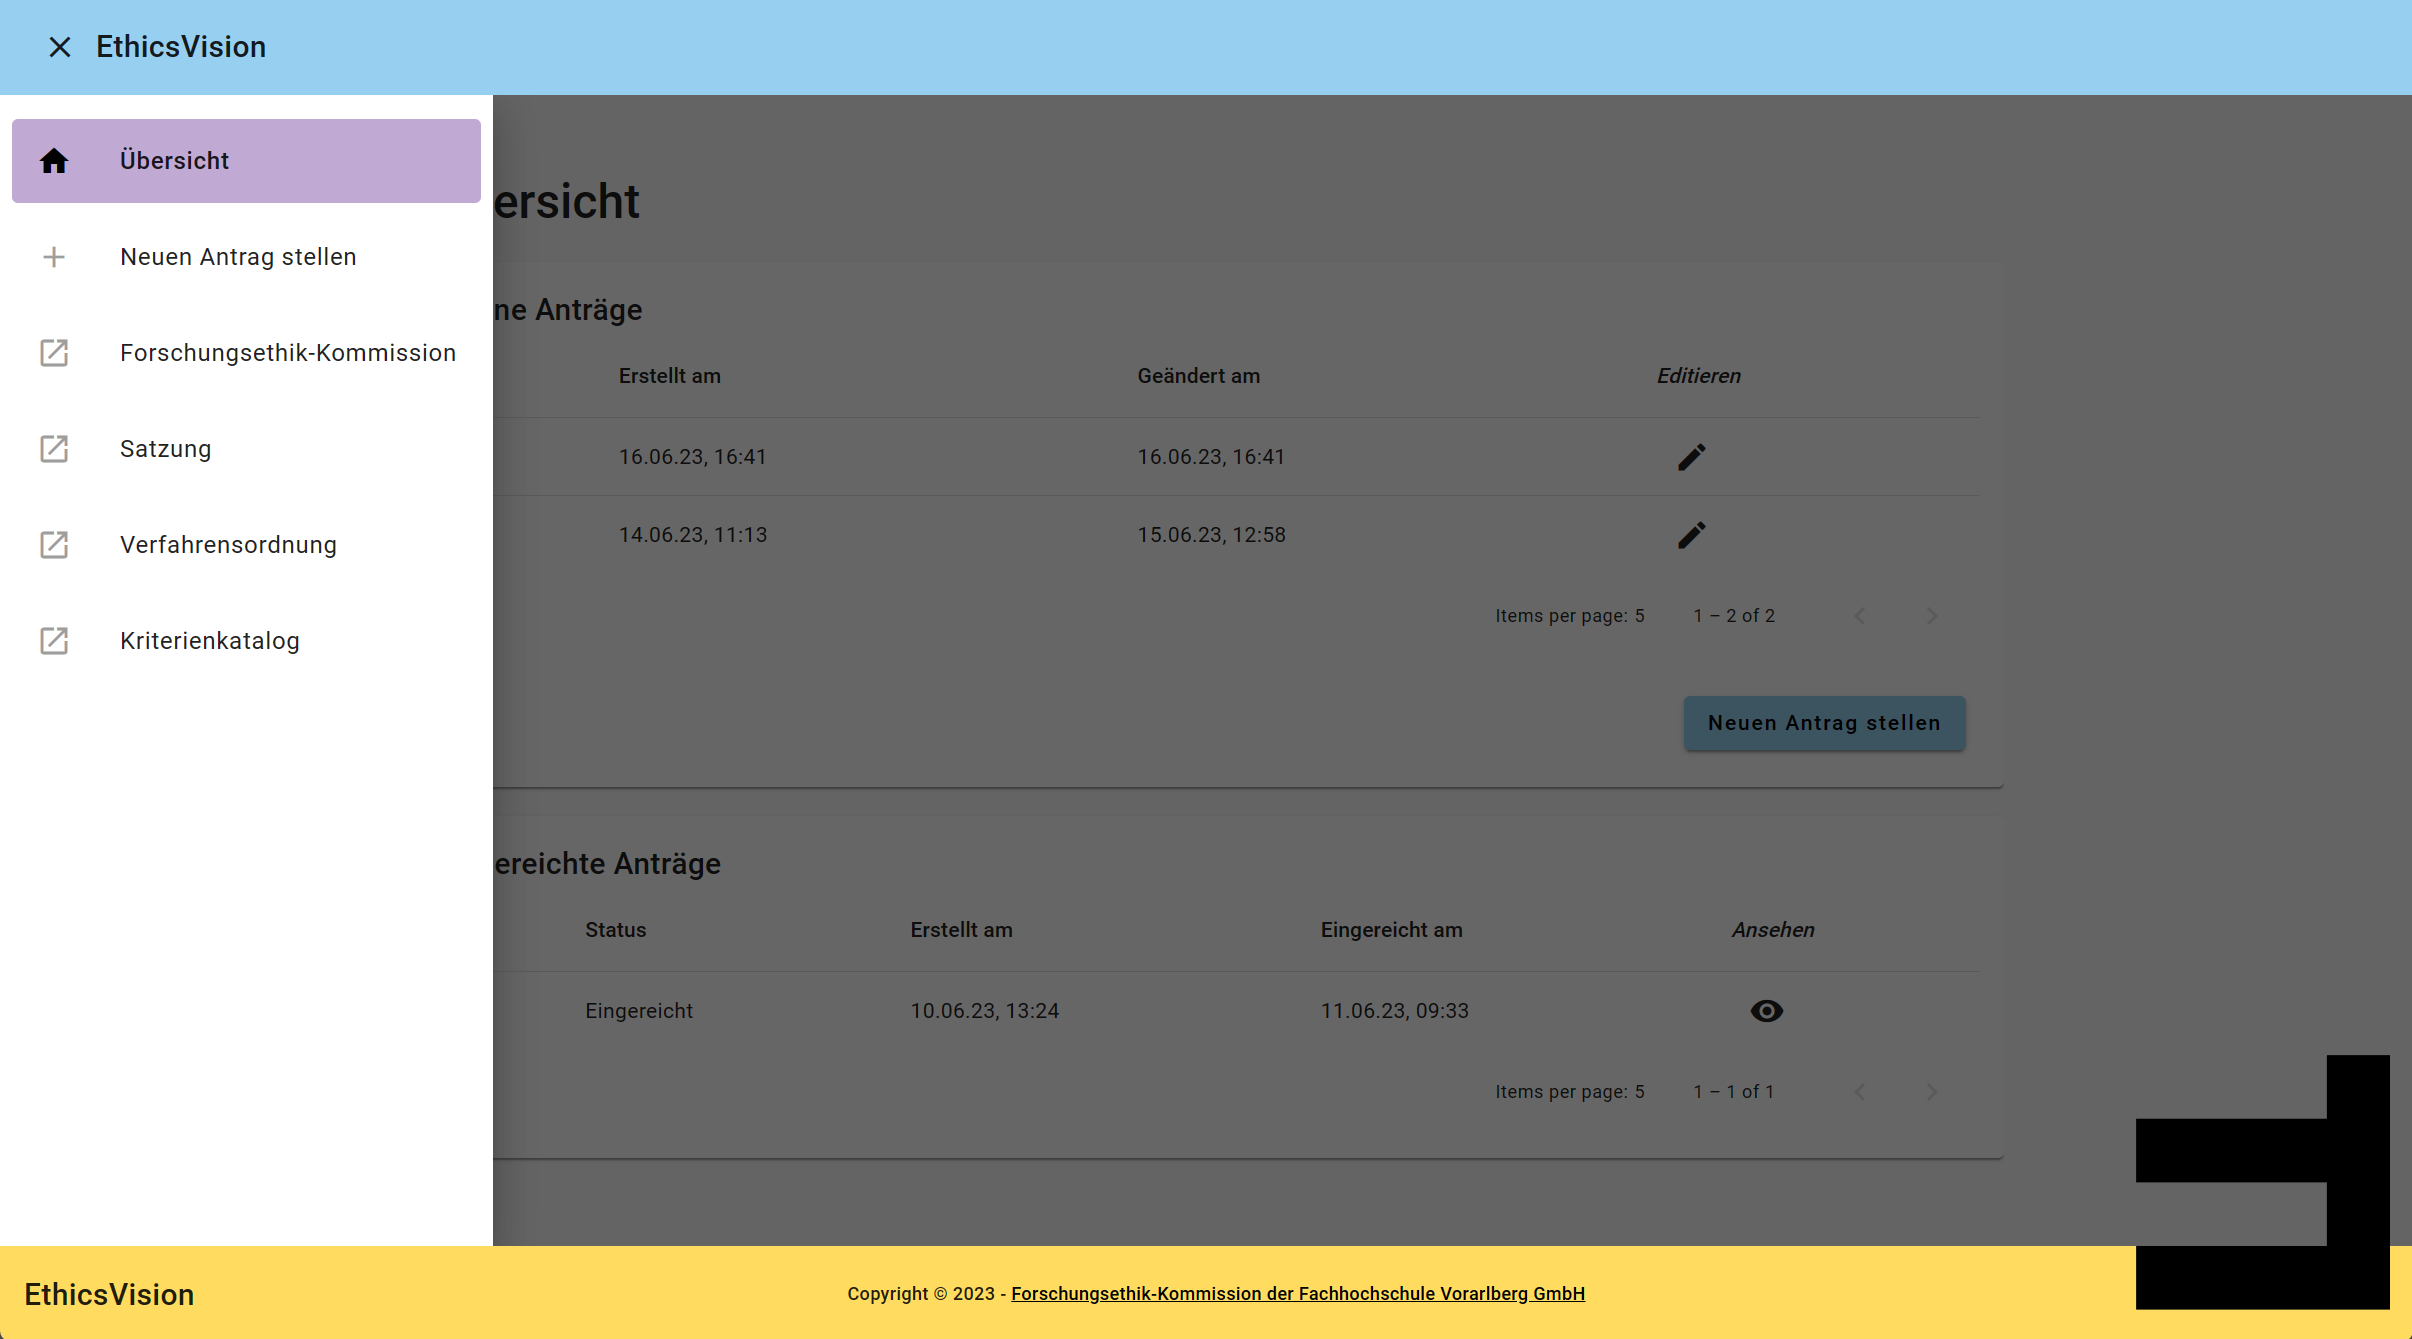
\includegraphics[width=\linewidth]{thesis/images/Luidold_EthicsVision-Übersicht_Menü.png}
    \caption{Seite \enquote{Übersicht} mit geöffnetem Seitenmenü}
    \label{fig:ethics-vision-übersicht-menü}
\end{figure}

\section{Abbildungen zum Formular"=Assistent}
\label{appendix:ethics-vision-formular-assistent}

\textbf{Anmerkung:} Der Formular"=Assistent wird Nutzer:innen im Rahmen der Erstellung eines neuen Ethikantrages angezeigt.

\begin{figure}[ht]
    \centering
    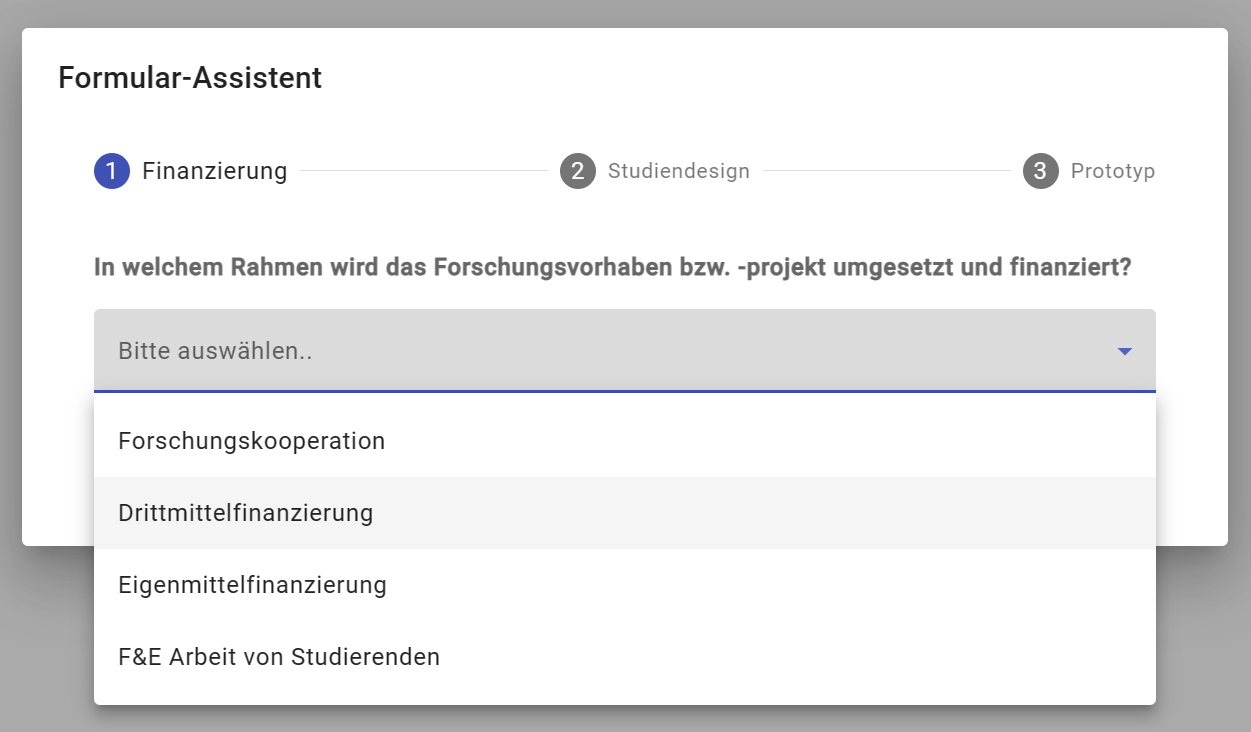
\includegraphics[width=.85\linewidth]{thesis/images/Luidold_EthicsVision-Formular-Assistent_Finanzierung.png}
    \caption{Schritt \#1 des Formular-Assistenten}
    \label{fig:ethics-vision-formular-assistent-finanzierung}
\end{figure}

\begin{figure}[ht]
    \centering
    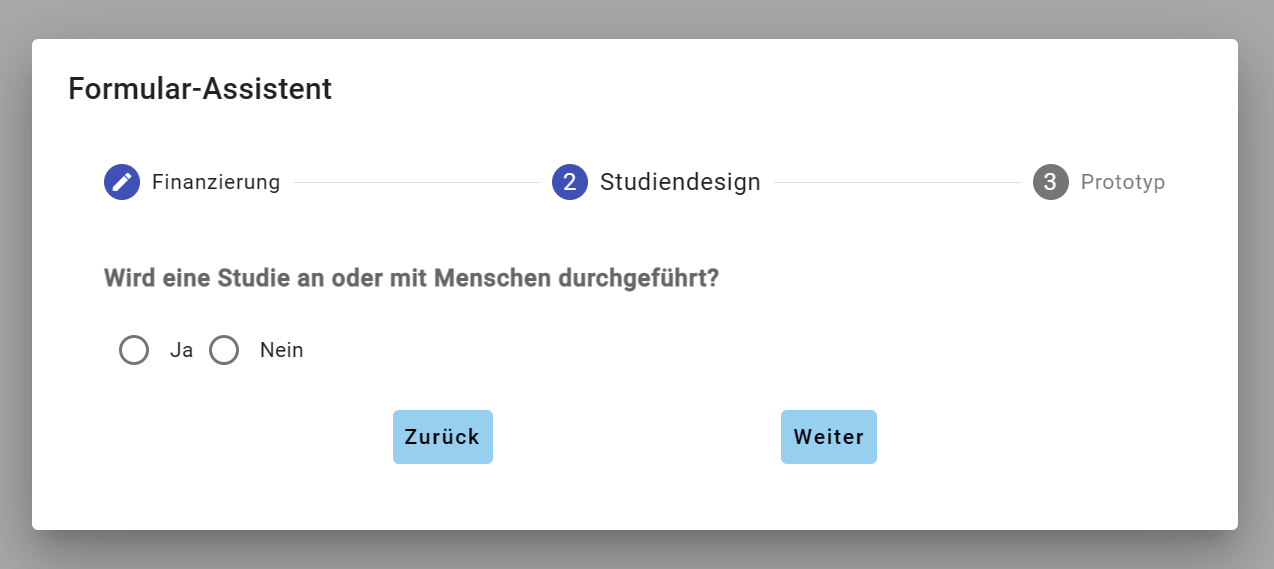
\includegraphics[width=.85\linewidth]{thesis/images/Luidold_EthicsVision-Formular-Assistent_Studiendesign.png}
    \caption{Schritt \#2 des Formular-Assistenten}
    \label{fig:ethics-vision-formular-assistent-studiendesign}
\end{figure}

\begin{figure}[ht]
    \centering
    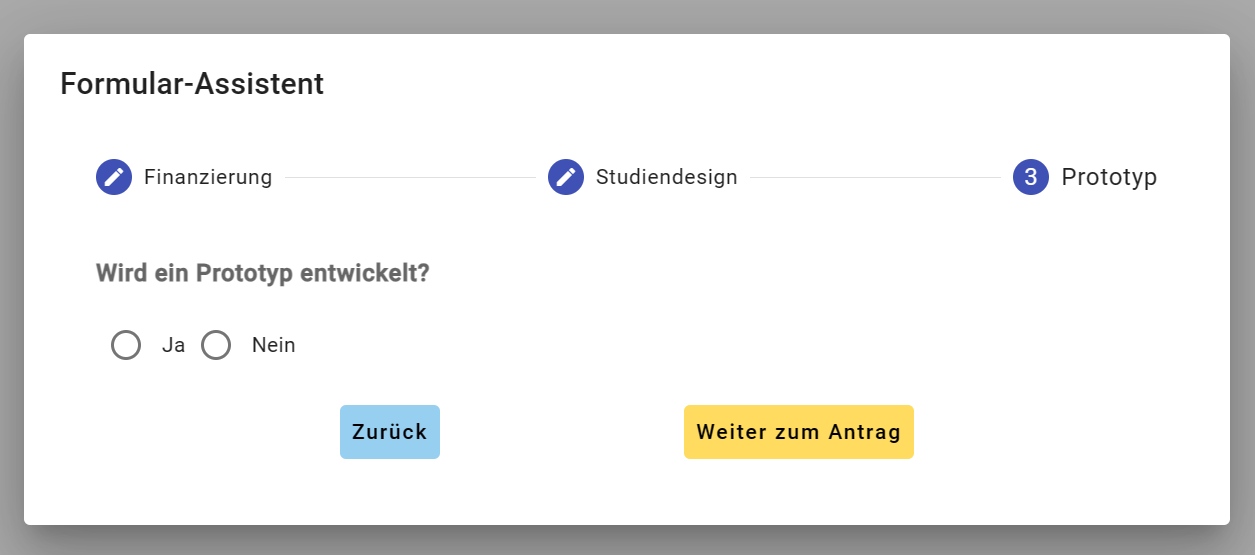
\includegraphics[width=.85\linewidth]{thesis/images/Luidold_EthicsVision-Formular-Assistent_Prototyp.png}
    \caption{Schritt \#3 des Formular-Assistenten}
    \label{fig:ethics-vision-formular-assistent-prototyp}
\end{figure}

\section{Abbildungen zum generierten Ethikantrag}
\label{appendix:ethics-vision-formular}

\textbf{Anmerkung:} Der dargestellte Ethikantrag wurde mit den Eingaben \texttt{F\&E-Arbeit von Studierenden} zur Frage \enquote{In welchem Rahemn wird das Forschungsvorhaben beziehungsweise -projekt umgesetzt und finanzeirt?}, \texttt{Ja} zur Frage \enquote{Wird eine Studie an oder mit Menschen durchgeführt?} und \texttt{Ja} zur Frage \enquote{Wird ein Prototyp entwickelt?} generiert.

\begin{figure}[ht]
    \centering
    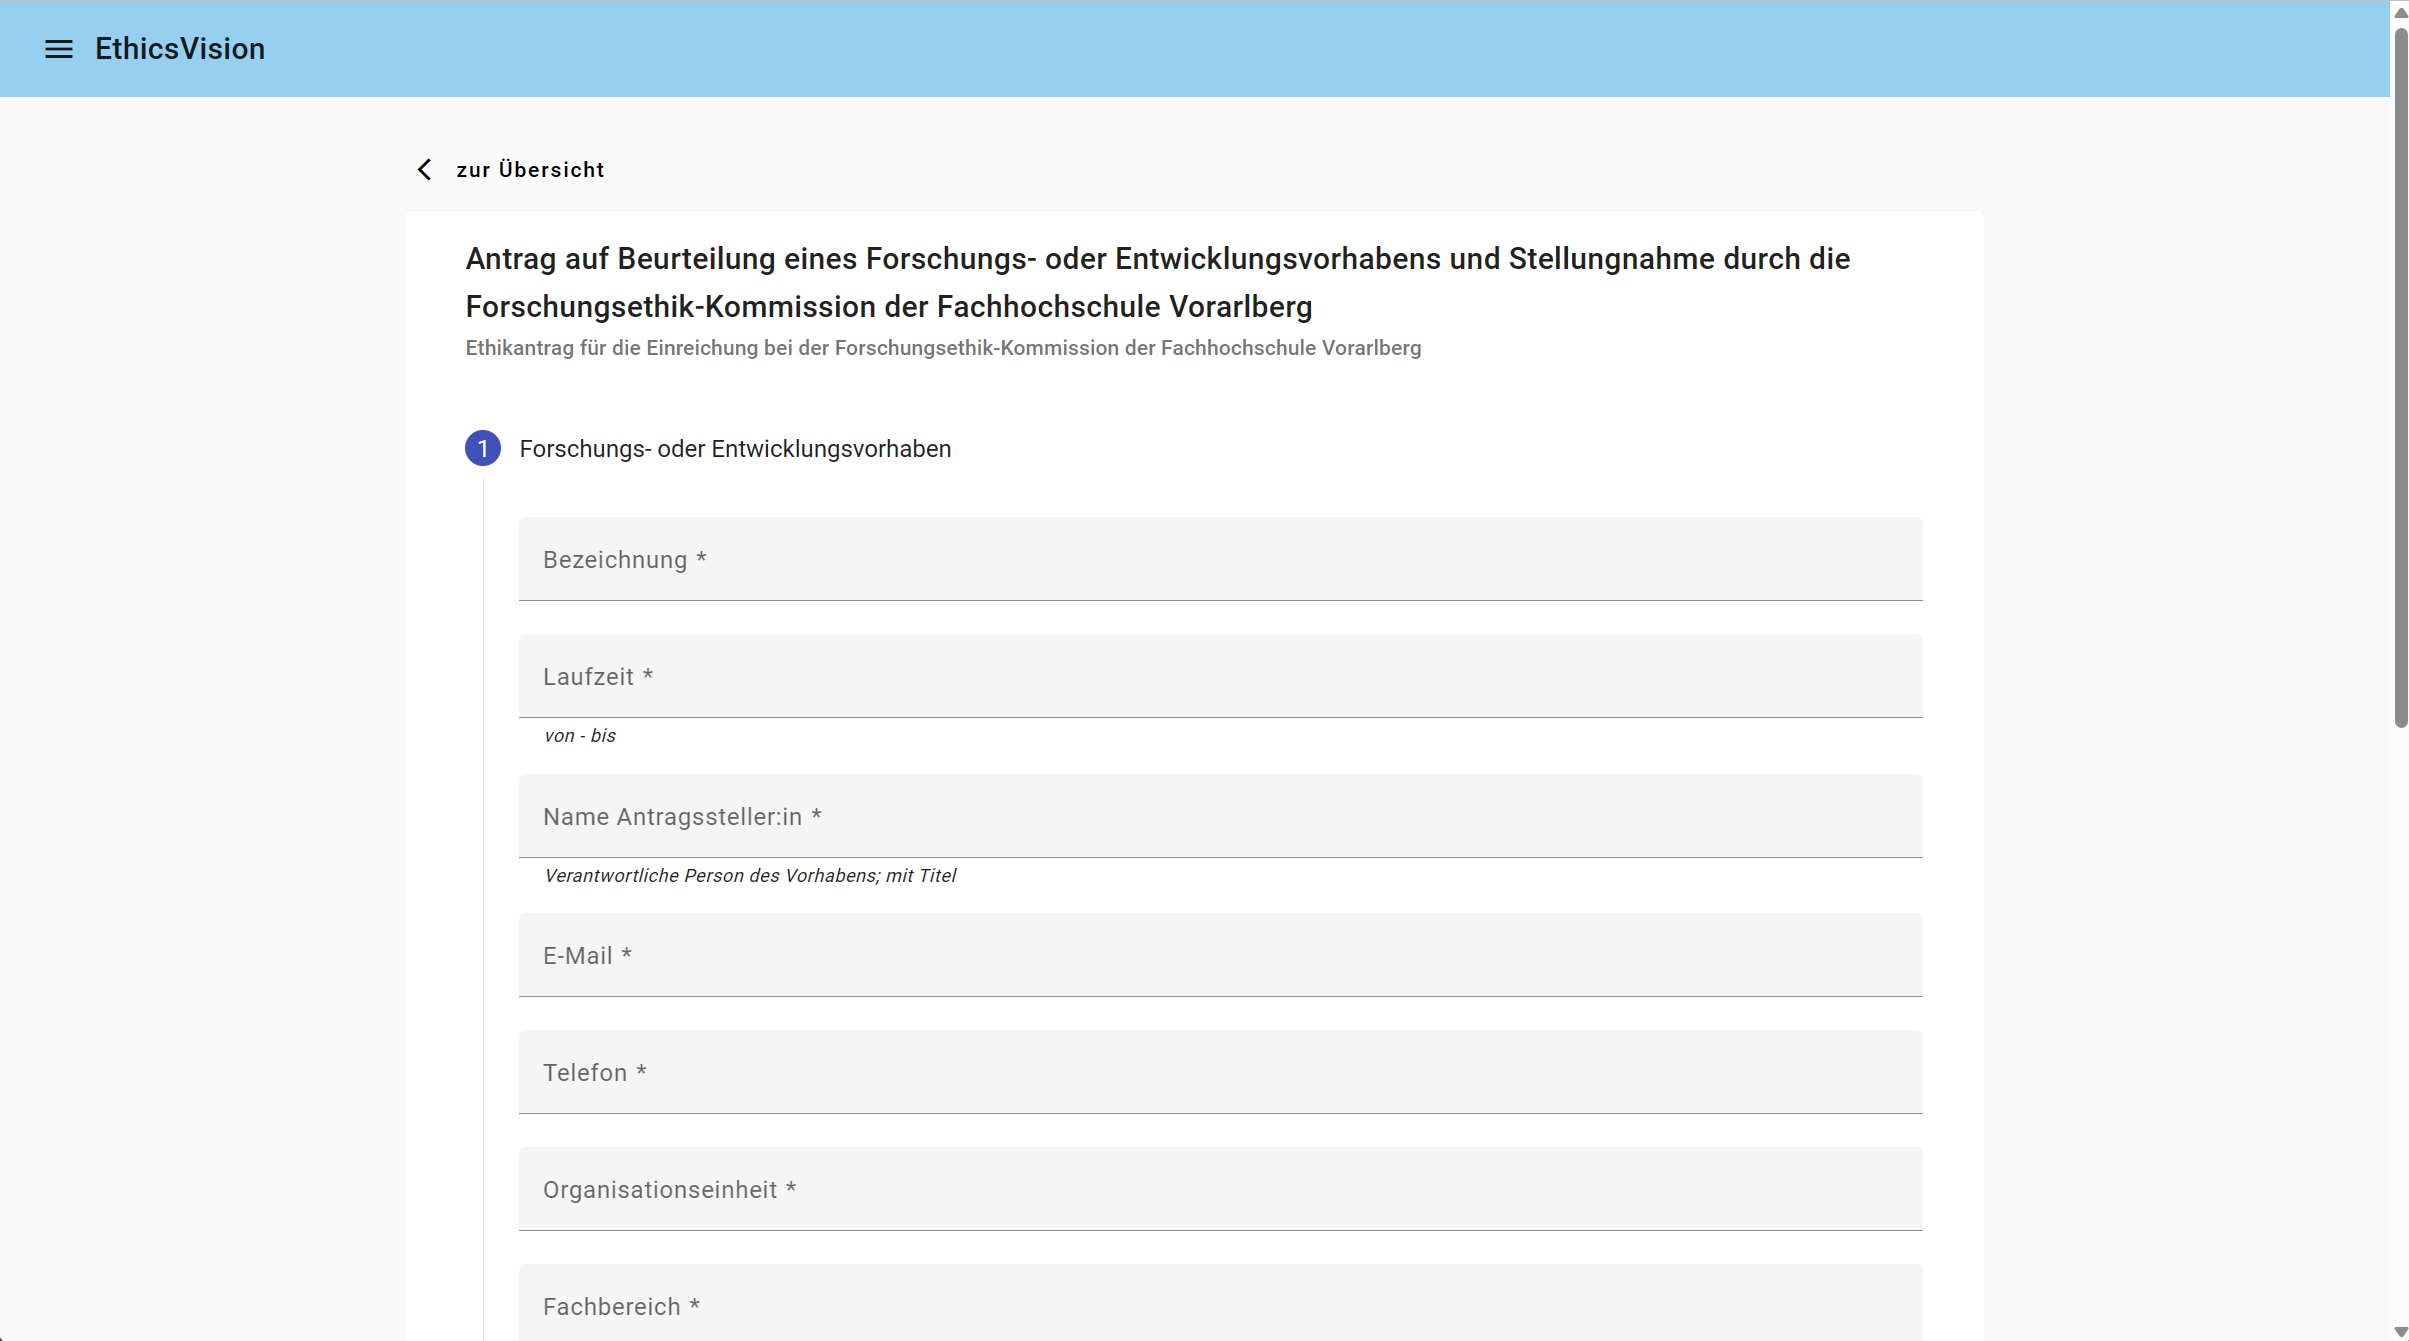
\includegraphics[width=\linewidth]{thesis/images/Luidold_EthicsVision-Formular_Start.png}
    \caption{Generierter Ethikantrag mit geöffnetem Abschnitt mit Fragen zum \enquote{Forschungs- oder Entwicklungsvorhaben}}
    \label{fig:ethics-vision-formular-start}
\end{figure}

\begin{figure}[ht]
    \centering
    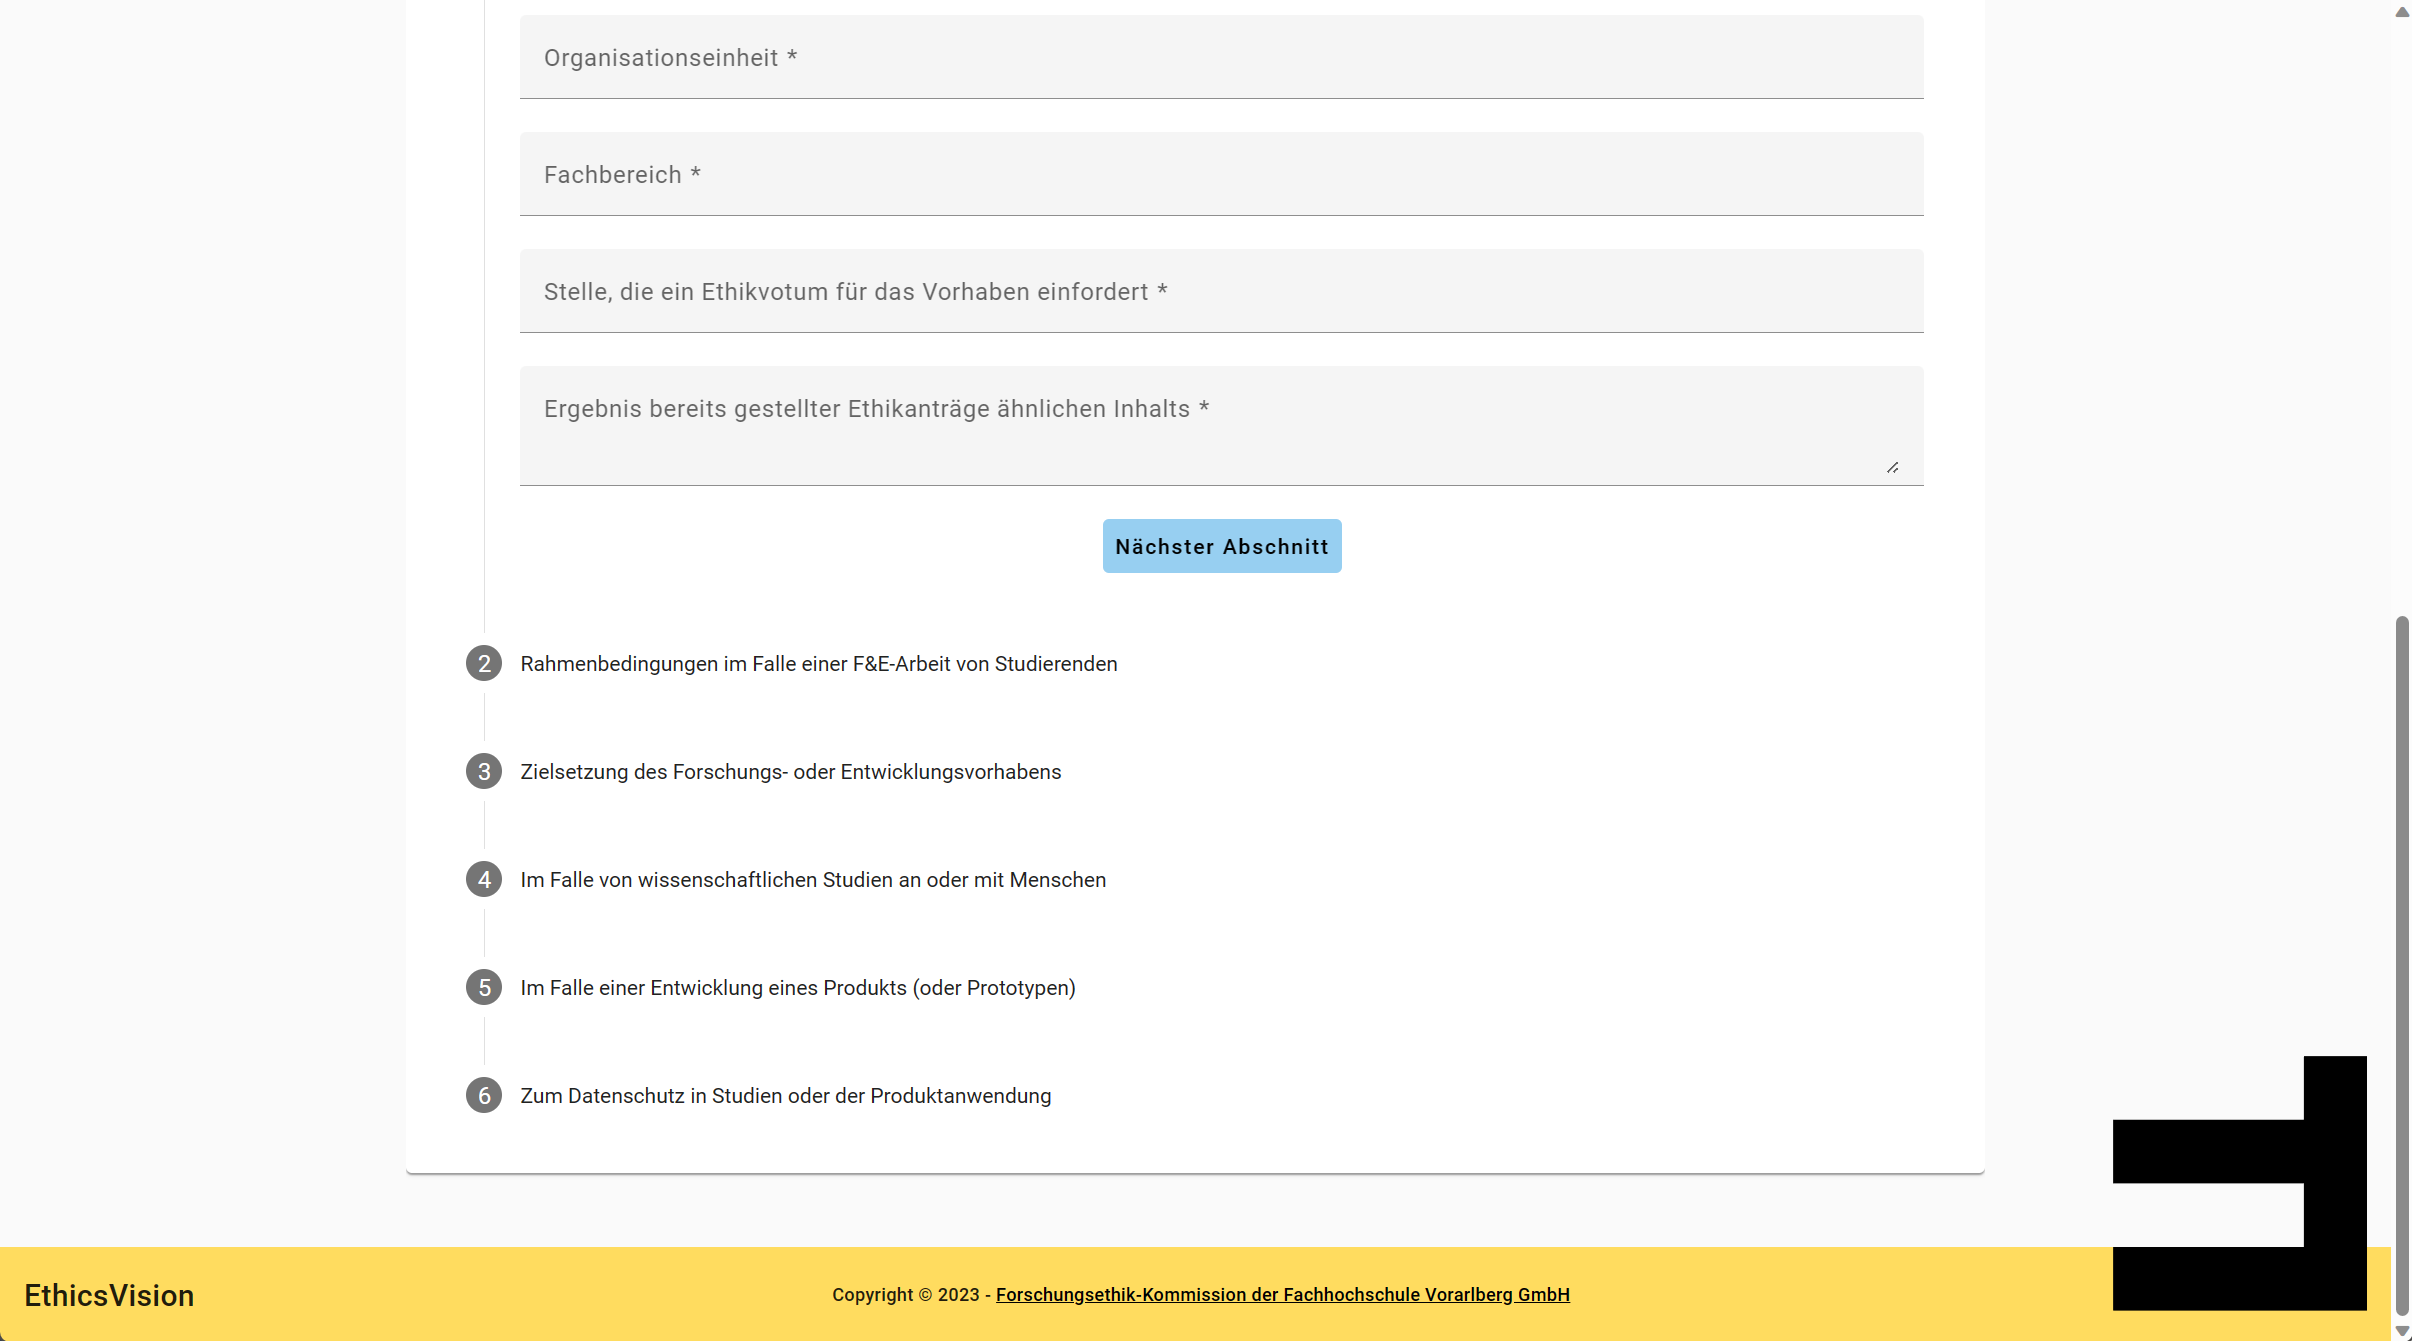
\includegraphics[width=\linewidth]{thesis/images/Luidold_EthicsVision-Formular_Ende.png}
    \caption{Generierter Ethikantrag mit Überblick über die weiteren inhaltlichen Themenblöcke}
    \label{fig:ethics-vision-formular-ende}
\end{figure}

\begin{figure}[ht]
    \centering
    \includegraphics[width=\linewidth]{thesis/images/Luidold_EthicsVision-Formular_unvollständig.png}
    \caption{Unvollständig ausgefüllter Ethikantrag mit sichtbaren Hinweisen zu Validierungsfehlern}
    \label{fig:ethics-vision-formular-unvollständig}
\end{figure}

% Eidesstattliche Erklärung
\clearpage
\chapter*{Eidesstattliche Erklärung}
\addcontentsline{toc}{chapter}{Eidesstattliche Erklärung}
Ich erkläre hiermit an Eides statt, dass ich die vorliegende Masterarbeit selbstständig und ohne Benutzung anderer als der angegebenen Hilfsmittel angefertigt habe. Die aus fremden Quellen direkt oder indirekt übernommenen Stellen sind als solche kenntlich gemacht. Die Arbeit wurde bisher weder in gleicher noch in ähnlicher Form einer anderen Prüfungsbehörde vorgelegt und auch noch nicht veröffentlicht.

\vspace{5cm}
\noindent
Dornbirn, am [Tag. Monat Jahr anführen]\hfill Dominic Luidold, BSc

\end{document}
